%%%%%%%%%%%%%%%%%%%%%%%%%%%%%%%%%%%%%%%%%%%%%%%%%%%%%%%%%%%%%%%%%%%%%%%%
%%                                                                    %%
%% This is file `ucalgarythesis.tex'  -- a document template for      %%
%% graduate theses at the University of Calgary.                      %%
%%                                                                    %%
%% This template document is to be used in conjunction with the       %%
%% thesis class file `ucalgarythesis.cls'.                            %%
%%                                                                    %%
%% Created by M.W. Girard, last updated 10 April 2016.                %%
%%                                                                    %%
%% This template was created to be in compliance with the University  %%
%% of Calgary thesis guidelines (version 14 April 2014)               %%
%%       https://grad.ucalgary.ca/current/thesis/guidelines.          %%
%%                                                                    %%
%%%%%%%%%%%%%%%%%%%%%%%%%%%%%%%%%%%%%%%%%%%%%%%%%%%%%%%%%%%%%%%%%%%%%%%%
%%                                                                    %%
%% By default, the text of the thesis is doublespaced and should be   %%
%% printed single-sided. All margins must be exactly one inch on all  %%
%% sides, and should not be bound or have binding edges. This is      %%
%% required by the University of Calgary thesis guidelines.           %%
%% All theses are now required to be submitted electronically.        %%
%%                                                                    %%
%%%%%%%%%%%%%%%%%%%%%%%%%%%%%%%%%%%%%%%%%%%%%%%%%%%%%%%%%%%%%%%%%%%%%%%%


%%%%%%%%%%%%%%%%%%%%%%%%%%%%%%%%%%%%%%%%%%%%%%%%%%%%%%%%%%%%
%%
%% Load the `ucalgarythesis.cls' document class
%%%%%%%%%%%%%%%%%%%%%%%%%%%%%%%%%%%%%%%%%%%%%%%%%%%%%%%%%%%%

\documentclass{ucalgarythesis}

%%%%%%%%%%%%%%%%%%%%%%%%%%%%%%%%%%%%%%%%%%%%%%%%%%%%%%%%%%%%%%%%%%%%%%
%% If you would like to print a personal copy of your thesis for    %%
%% your own record, you may print it double-sided and with extra    %%
%% margins for binding. Use the following line instead of the above %%
%% \documentclass{ucalgarythesis} for compiling personal copies of  %%
%% the thesis to be printed double-sided and bound.                 %%
%%%%%%%%%%%%%%%%%%%%%%%%%%%%%%%%%%%%%%%%%%%%%%%%%%%%%%%%%%%%%%%%%%%%%%
%\documentclass[twoside,binding]{ucalgarythesis}

%%%%%%%%%%%%%%%%%%%%%%%%%%%%%%%%%%%%%%%%%%%%%%%%%%%%%%%%%%%%
%%
%% Imported packages & custom user commands
%%%%%%%%%%%%%%%%%%%%%%%%%%%%%%%%%%%%%%%%%%%%%%%%%%%%%%%%%%%%

%% Include extra packages here

\usepackage[utf8]{inputenc}
\usepackage{amssymb,amsthm,amsmath}
%\usepackage[hidelinks]{hyperref}
\usepackage{algorithm}
%\usepackage{algorithmic}
\usepackage{algpseudocode}
\usepackage{comment}
\usepackage{enumitem}
\usepackage{graphicx}
\usepackage{multirow}
\usepackage{hyperref}
\usepackage{pgfplots}
\usepackage{tikz-cd}
\usepackage[style=numeric, backend=biber]{biblatex}
\bibliography{biblio}
%\bibliographystyle{plain}

%\usepackage{biblatex}

\hypersetup{
    colorlinks,
    citecolor=blue,
    filecolor=blue,
    linkcolor=blue,
    urlcolor=blue
}

%%  Include other user-defined commands here

\let\div\undefined
\renewcommand{\bar}{\overline}

\algnewcommand{\algorithmicgoto}{\textbf{go to}}
\algnewcommand{\GoTo}[1]{\algorithmicgoto~{#1}}

\DeclareMathOperator{\Char}{char}
\DeclareMathOperator{\Cl}{Cl}
\DeclareMathOperator{\coeff}{coeff}
\DeclareMathOperator{\coim}{coim}
\DeclareMathOperator{\coker}{coker}
\DeclareMathOperator{\Der}{Der}
\DeclareMathOperator{\Div}{Div}
\DeclareMathOperator{\div}{div}
\DeclareMathOperator{\Frac}{Frac}
\DeclareMathOperator{\Gal}{Gal}
\DeclareMathOperator{\Hom}{Hom}
\DeclareMathOperator{\Id}{Id}
\DeclareMathOperator{\im}{im}
\DeclareMathOperator{\lcm}{lcm}
\DeclareMathOperator{\Jac}{Jac}
\DeclareMathOperator{\LM}{LM}
\DeclareMathOperator{\LT}{LT}
\DeclareMathOperator{\Ker}{Ker}
\DeclareMathOperator{\nullity}{null}
\DeclareMathOperator{\Pic}{Pic}
\DeclareMathOperator{\Princ}{Princ}
\DeclareMathOperator{\RGB}{RGB}
\DeclareMathOperator{\orb}{orb}
\DeclareMathOperator{\ord}{ord}
\DeclareMathOperator{\rank}{rank}
\DeclareMathOperator{\supp}{supp}
\DeclareMathOperator{\Span}{Span}
\DeclareMathOperator{\type}{type}
%\DeclareMathOperator{\KVec}{K-Vec}

\newcommand{\inv}{^{-1}}
\newcommand{\pid}[1]{\left\langle #1 \right\rangle}

%\newcommand{\der}{\partial}
\newcommand{\defn}{\textbf}
\newcommand{\note}[1]{{\color{red}#1}}
\newcommand{\bb}[1]{\mathbb{#1}}
\newcommand{\tensor}[1]{\underset{#1}{\otimes}}
\renewcommand{\cal}[1]{\mathcal{#1}}

\numberwithin{equation}{section}
\numberwithin{figure}{section}
\numberwithin{table}{section}

\theoremstyle{plain}
\newtheorem{theorem}[equation]{Theorem}
\newtheorem{corollary}[equation]{Corollary}
\newtheorem{conjecture}[equation]{Conjecture}
\newtheorem{lemma}[equation]{Lemma}
\newtheorem{proposition}[equation]{Proposition}

\theoremstyle{definition}
\newtheorem{definition}[equation]{Definition}
\newtheorem{example}[equation]{Example}
\newtheorem{remark}[equation]{Remark}

\renewcommand*{\arraystretch}{0.8} % Adjust spacing between lines in matrices

\renewcommand\thesection{\arabic{section}} % Fix section/subsection numbering style
\renewcommand\thesubsection{\thesection.\arabic{subsection}}

%%%%%%%%%%%%%%%%%%%%%%%%%%%%%%%%%%%%%%%%%%%%%%%%%%%%%%%%%%%%%%%%%%%%%%%%
%%                                                                    %%
%% Begin document                                                     %%
%%                                                                    %%
%%%%%%%%%%%%%%%%%%%%%%%%%%%%%%%%%%%%%%%%%%%%%%%%%%%%%%%%%%%%%%%%%%%%%%%%
\begin{document}

%%%%%%%%%%%%%%%%%%%%%%%%%%%%%%%%%%%%%%%%%%%%%%%%%%%%%%%%%%%%%%%%%%%%%%%%
%%                                                                    %%
%% Title page                                                         %%
%%                                                                    %%
%%%%%%%%%%%%%%%%%%%%%%%%%%%%%%%%%%%%%%%%%%%%%%%%%%%%%%%%%%%%%%%%%%%%%%%%

%%%%%%%%%%%%%%%%%%%%%%%%%%%%%%%%%%%%%%%%%%%%%%%%%%%%%%%%%%%%%%%%%%%%%%%%
%% Instructions for title page information:                           %%
%%                                                                    %%
%%  Fill in the following fields with the required information:       %%
%%   - \title{...}        Title of the thesis                         %%
%%   - \author{...}       Your full name                              %%
%%   - \thesis{Thesis}    Type of document (may change to `Thesis' to %%
%%                           `Dissertation' depending on type of work)%%
%%   - \dept{...}         Full name of the graduate department or     %%
%%                           degree program                           %%
%%   - \degree{...}       Full name of the degree obtained            %%
%%                          (i.e. Doctor of Philosophy,               %%
%%                                 Master of Science, etc)            %%
%%   - \gradyear{...}     Year of submission                          %%
%%   - \monthname{...}    Month of submission                         %%
%%%%%%%%%%%%%%%%%%%%%%%%%%%%%%%%%%%%%%%%%%%%%%%%%%%%%%%%%%%%%%%%%%%%%%%%

\title{Divisor Class Group Arithmetic on $C_{3,4}$ Curves}
 
\author{Evan MacNeil}
\thesis{Thesis}
\dept{Graduate Program in Mathematics and Statistics}
\degree{Master of Science}
\gradyear{2019}
\monthname{August}


%%%%%%%%%%%%%%%%%%%%%%%%%%%%%%%%%%%%%%%%%%%%%%%%%%%  
%% Make the thesis title page.
%%%%%%%%%%%%%%%%%%%%%%%%%%%%%%%%%%%%%%%%%%%%%%%%%%%
\frontmatter           %% Don't remove this line.
\makethesistitle       %% Don't remove this line.


%%%%%%%%%%%%%%%%%%%%%%%%%%%%%%%%%%%%%%%%%%%%%%%%%%%%%%%%%%%%%%%%%%%%%%%%
%%                                                                    %%
%% Prefatory pages                                                    %%
%%                                                                    %%
%%%%%%%%%%%%%%%%%%%%%%%%%%%%%%%%%%%%%%%%%%%%%%%%%%%%%%%%%%%%%%%%%%%%%%%%
%% The following sections are in the correct order as specified by    %%
%% the April 2014 thesis guidelines set by the University of Calgary. %%
%%                                                                    %%
%% You may remove optional sections, but do not change the order.     %%
%%%%%%%%%%%%%%%%%%%%%%%%%%%%%%%%%%%%%%%%%%%%%%%%%%%%%%%%%%%%%%%%%%%%%%%%

%%%%%%%%%%%%%%%%%%%%%%%%%%%%%%%%%%%%%%%%%%%%%%%%%%%
%%
%% Abstract page (REQUIRED)
%%%%%%%%%%%%%%%%%%%%%%%%%%%%%%%%%%%%%%%%%%%%%%%%%%%

\begin{thesisabstract}  

Computing in the divisor class group of an algebraic curve is a non-trivial component in computing $L$-series.
$L$-series in turn are at the heart of the Sato-Tate conjecture and related conjectures.
The Sato-Tate conjecture has been proven for elliptic curves with complex multiplication,
but remains open for other families of algebraic curves.
In order to test these conjectures against other curve families, it is desirable to have efficient algorithms to perform divisor class group arithmetic.

Fast explicit formulas exist to perform divisor class group arithmetic for genus 1 and genus 2 curves.
However, the picture for genus 3 curves is incomplete.
Existing explicit formulas for arithmetic on non-hyperelliptic genus 3 curves ($C_{3,4}$ curves) have been developed with cryptographic applications in mind.
They make certain generacity assumptions on their inputs that hold with high probability in cryptographic settings,
but are unsuited for number theoretic use cases.
More general algorithms exist that can perform divisor class arithmetic over any curve, but they are slow.
The goal of this project is to bridge the gap --
to find fast explicit formulas describing $C_{3,4}$ curve arithmetic that are correct for all inputs.

\end{thesisabstract}


%%%%%%%%%%%%%%%%%%%%%%%%%%%%%%%%%%%%%%%%%%%%%%%%%%%
%%
%% Preface page (OPTIONAL)
%%%%%%%%%%%%%%%%%%%%%%%%%%%%%%%%%%%%%%%%%%%%%%%%%%%

%% This section is required if the work presented in the thesis is 
%% done as part of a collaboration. In this case, the preface must 
%% state which part of the thesis are the author's original work.
%% Otherwise this section is optional.

  \chapter{Preface}
 
  This thesis is an original work by the author. No part of this thesis has been previously published.
 
  % Some of the research conducted for this thesis forms part of an international research collaboration, led by Professor R.C. Smith at the University of Hogwarts
   
 
%%%%%%%%%%%%%%%%%%%%%%%%%%%%%%%%%%%%%%%%%%%%%%%%%%%
%%
%% Acknowledgements page (REQUIRED)
%%%%%%%%%%%%%%%%%%%%%%%%%%%%%%%%%%%%%%%%%%%%%%%%%%%

  \chapter{Acknowledgements}  
  
    [Don't forget to thank someone.]
    
%%%%%%%%%%%%%%%%%%%%%%%%%%%%%%%%%%%%%%%%%%%%%%%%%%
%%
%% Dedication page (this section is OPTIONAL)
%%%%%%%%%%%%%%%%%%%%%%%%%%%%%%%%%%%%%%%%%%%%%%%%%%

  \chapter[Dedication]{}
  
  \begin{dedication}
     \emph{To all the time I've wasted...}
  \end{dedication}

%%%%%%%%%%%%%%%%%%%%%%%%%%%%%%%%%%%%%%%%%%%%%%%%%%
%%
%% Various lists
%%%%%%%%%%%%%%%%%%%%%%%%%%%%%%%%%%%%%%%%%%%%%%%%%%
%% The Table of Contents and all Lists should be single spaced.

  \begin{singlespace}   %% Do not remove this line

%%%%%%%%%%%%%%%%%%%%%%%%%%%%%%%%%%%%%%%%%%%%%%%%%%
%%
%% Table of Contents (REQUIRED)
%%%%%%%%%%%%%%%%%%%%%%%%%%%%%%%%%%%%%%%%%%%%%%%%%%
  \renewcommand\contentsname{Table of Contents}
  \cleardoublepage\phantomsection
  \addcontentsline{toc}{chapter}{\contentsname}
  \tableofcontents

%%%%%%%%%%%%%%%%%%%%%%%%%%%%%%%%%%%%%%%%%%%%%%%%%%
%% List of figures (required, if any)
  \renewcommand{\listfigurename}{List of Figures and Illustrations}
  \cleardoublepage\phantomsection
  \addcontentsline{toc}{chapter}{\listfigurename}
  \listoffigures

%%%%%%%%%%%%%%%%%%%%%%%%%%%%%%%%%%%%%%%%%%%%%%%%%%
%% List of tables (required, if any)
  \renewcommand{\listtablename}{List of Tables}
  \cleardoublepage\phantomsection
  \addcontentsline{toc}{chapter}{\listtablename}
  \listoftables
  
%%%%%%%%%%%%%%%%%%%%%%%%%%%%%%%%%%%%%%%%%%%%%%%%%%
%% List of Symbols, abbreviations, and nomenclature (required, if any)   
%%
%% (Note: You may use your own format for your list of symbols, 
%%  abbreviations, etc. This format is just a guideline.)
%%
  \chapter{List of Symbols, Abbreviations and Nomenclature}      
  \begin{tabbing}
    Symbol or abbreviation~~~~~\= \ \ \ \ \ \ \ \ \ \ \ \ \ \ \ \ \ \ \ \ \ \ \ \ \ \ \ \ \ \ \ \ \ \ \ \  \parbox{5in}{Definition}\\

    \addsymbol \mbox{$\alpha$}: {The first letter of the Greek alphabet}
    \addsymbol \mbox{$\beta$}: {The second letter of the Greek alphabet}
    %
    % Add more symbols here...
    % . 
    % .
    % .
    %
    
    % Always keep the following line if you are using a list of symbols:
  \end{tabbing}
  
%%%%%%%%%%%%%%%%%%%%%%%%%%%%%%%%%%%%%%%%%%%%%%%%%%
%% End single spacing after last list
  \end{singlespace}     %% Do not remove this line
  
%%%%%%%%%%%%%%%%%%%%%%%%%%%%%%%%%%%%%%%%%%%%%%%%%%
%
% Epigraph (this section is OPTIONAL)
%%%%%%%%%%%%%%%%%%%%%%%%%%%%%%%%%%%%%%%%%%%%%%%%%%

  \chapter{Epigraph}

  \begin{epiquote} 
   \textit{A quotation is a handy thing to have about, saving one the trouble of thinking for oneself, always a laborious business.} 
  \end{epiquote}    
  \begin{flushright} - A.A. Milne, \textit{If I May}\end{flushright}\bigskip
   

%%%%%%%%%%%%%%%%%%%%%%%%%%%%%%%%%%%%%%%%%%%%%%%%%%%%%%%%%%%%%%%%%%%%%%%%
%%                                                                    %%
%% Main matter                                                        %%
%%                                                                    %%
%%%%%%%%%%%%%%%%%%%%%%%%%%%%%%%%%%%%%%%%%%%%%%%%%%%%%%%%%%%%%%%%%%%%%%%%

  \mainmatter           %% Do not remove this line
    
%%%%%%%%%%%%%%%%%%%%%%%%%%%%%%%%%%%%%%%%%%%%%%%%%%
%%
%% Chapters
%%%%%%%%%%%%%%%%%%%%%%%%%%%%%%%%%%%%%%%%%%%%%%%%%%

\setcounter{page}{12}

%%%%%%%%%%%%%%%%%%%%%%%%%%
%%%%%                %%%%%
%%%%%   Background   %%%%%
%%%%%                %%%%%
%%%%%%%%%%%%%%%%%%%%%%%%%%

\section{Introduction}

This introduction will be light on definitions.
Full details of the topics mentioned may be found later in this thesis or in other cited works.
For now, it should be enough to know that an \defn{algebraic plane curve} is the set of points $(x,y)$
at which $f(x, y) = 0$, for some field $K$ and polynomial $f \in K[x,y]$.
Examples of algebraic plane curves include elliptic curves, hyperelliptic curves,
and the subject of this thesis, $C_{3,4}$ curves.
An \defn{elliptic curve} is the set of zeroes of a polynomial
\begin{equation}
  \label{eq_elliptic}
  y^2 + x^3 + c_4xy + c_3x^2 + c_2y + c_1x + c_0.
\end{equation}
A (ramified genus 3) \defn{hyperelliptic curve} is the set of zeroes of a polynomial
\begin{equation}
  \label{eq_genus_3_hyperelliptic}
  y^2 + x^7 + c_{10}x^3y + c_9x^6 + c_8x^2y + c_7x^5 + c_6xy + c_5x^4 + c_4y + c_3x^3 + c_2x^2 + c_1x + c_0,
\end{equation}
though hyperelliptic curves can be of any genus 2 or greater and come in a variety of flavours (ramified, split, inert).
A \defn{$C_{3,4}$ curve} is the set of zeroes of a polynomial
\begin{equation}
  \label{eq_c34_intro}
  y^3 + x^4 + c_8xy^2 + c_7x^2y + c_6x^3 + c_5y^2 + c_4xy + c_3x^2 + c_2y + c_1x + c_0.
\end{equation}
For each of these classes of curves, one might also demand that they be non-singular
\note{(put a definition of singular in chapter 4 and refer to it here)},
as we will do in Chapter \ref{chap_curves}.

If $C$ is an algebraic plane curve, a \defn{divisor} of a curve is a formal sum of points on $C$.
If $P$ and $Q$ are points on $C$, then $2P$ and $P - Q$ are examples of divisors on $C$.
In Chapter \ref{chap_divisors}, we will place an equivalence relation on divisors,
partitioning them into \defn{divisor classes}.
Together with an addition operation, this forms the \defn{divisor class group} of $C$.



%%%%%%%%%%%%%%%%%%%%%%%%%%
%%%%%                %%%%%
%%%%%   Motivation   %%%%%
%%%%%                %%%%%
%%%%%%%%%%%%%%%%%%%%%%%%%%

\subsection{Motivation}

Let $\bb F_q$ be the finite field of order $q$ and suppose $E$ is an elliptic curve defined over $\bb F_q$,
meaning that $E$ is the set of zeroes of a polynomial in $\bb F_q[x,y]$ of the form in Equation \ref{eq_elliptic}.
The following theorem, due to Helmut Hasse (1898 -- 1979), says that
the number of rational points (i.e. points in $\bb F_q \times \bb F_q$) on $E$
lies in some interval that is small compared to the order of $\bb F_q$.
\begin{theorem}[Hasse]
  Let $E$ be an elliptic curve over a finite field $\bb F_q$.
  The number of rational points on $E$ differs from $q + 1$ by at most $2 \sqrt q$. That is,
  \[ | \#E(\bb F_q) - (q + 1) | \leq 2 \sqrt q. \]
\end{theorem}
In other words,
$q + 1$ is a good estimate for the number of rational points on $E$,
especially when $q$ is large.

\begin{example}
  Let $p = 2^{31} - 1 = 2,147,483,647$, which is prime.
  The elliptic curve $y^2 + x^3 - 1 = 0$ over $\bb F_p[x,y]$ has 2,147,391,324 rational points.
\end{example}

Let $a_q = \frac {\#E(\bb F_q) - (q + 1)} {2\sqrt q}$.
Then Hasse's Theorem says that $a_p \in [-1, 1]$.
Letting $\theta_q = \arccos a_q$, then $\theta_q \in [0, \pi]$.
Given a subinterval $[\alpha, \beta] \subseteq [0, \pi]$ and a prime $p$,
one can ask what the probabilty is that $\theta_p \in [\alpha, \beta]$.
The Sato-Tate Conjecture suggests that, for most elliptic curves, this probability follows a $\sin^2$ distribution.

\begin{conjecture}[Sato-Tate, \cite{silverman92}]
  Let $E$ be an elliptic curve over $\bb Q$ without complex multiplication.
  For any interval $[\alpha, \beta] \subseteq [0, \pi]$
  \[ \lim_{N \to \infty}
    \frac {\#\{ p \leq N : \alpha \leq \theta_p \leq \beta \}} {\pi(N)} =
    \frac 2 \pi \int_{\alpha}^{\beta} \sin^2 \theta\,d\theta, \]
  where $p$ is prime and $\pi(N)$ is the prime-counting function.
\end{conjecture}

This conjecture on the number of points on an elliptic curve $E$
can be made into a statement about the $L$-series of $E$.
\begin{comment}
The $L$-series of curves are central to many conjectures in number theory.
A complete discussion of $L$-series is outside the scope of this thesis;
we present only enough to motivate the topic of this thesis.
Let $E$ be an elliptic curve defined over the rational numbers $\bb Q$,
meaning $E$ is defined by a polynomial in $\bb Q[x,y]$ of the form of Equation \ref{eq_elliptic}.
\end{comment}
The \defn{$L$-series} of $E$ is defined as
\[ L(E/\bb Q, s)  = \prod_{p \text{ is prime}} \frac 1 {L_p \left( \frac 1 {p^s} \right)},\]
where, for each prime $p$, $L_p$ is a non-zero polynomial in $\bb Q[t]$ of degree at most 2.
For more on $L$-series, including a precise definition of the polynomials $L_p$,
see \cite{husemoller87}, \cite{milne06}, or \cite{silverman09}.

If $E/\bb Q$ has ``good reduction'' at a prime $p$
(see again \cite{husemoller87}, \cite{milne06}, or \cite{silverman09}),
then $L_p(1) = \#E(\bb F_p)$, which is the value of interest in the Sato-Tate Conjecture.

There are many other important number-theoretic conjectures related to the $L$-series of an elliptic curve.
One of the Clay Mathematics Institute's seven famous Millenium Prize Problems,
with a \$1,000,000 bounty on its head,
is the Birch and Swinnerton-Dyer Conjecture.

\begin{conjecture}[Birch and Swinnerton-Dyer, \cite{koblitz93}]
  Let $E$ be an elliptic curve over $\bb Q$.
  Then $L(E/\bb Q, s)$ has a zero at $s = 1$ of order equal to the rank of $E(\bb Q)$.
\end{conjecture}

In order to test this conjecture against a given curve $E/\bb Q$,
one may wish to compute $L(E, 1)$, which requires computing $L_p(\frac 1 p)$ at many primes $p$,
in turn requiring one to count points on many elliptic curves.

Hasse's Theorem has a generalization to higher genus curves
(elliptic curves have genus 1) that is easy to state.
\begin{theorem}[Hasse-Weil]
  Let $C$ be an algebraic curve of genus $g$ over a finite field $\bb F_q$.
  The number of points on $C$ differs from $q + 1$ by at most $2g \sqrt q$.
  That is,
  \[ | \#E(\bb F_q) - (q + 1) | \leq 2g \sqrt q. \]
\end{theorem}

The Sato-Tate Conjecture and the Birch and Swinnerton-Dyer conjectures
(and other $L$-series-related conjectures not mentioned above,
including the Koblitz-Zywina conjecture and Lang-Trotter conjecture)
also have generalizations to higher genus curves \cite{sutherland16} \cite{sutherland18}.
However, on higher-genus curves, $L_p(1)$ is no longer the number of points on the curve,
but rather the order of the divisor class group of the curve \cite{kedlaya08},
which is known to be a finite Abelian group.
(In the case of elliptic curves, the order of the divisor class group is
equal to the number of points on the curve.)

To compute the order of a finite Abelian group, one may first compute the order of an element of that group
using an algorithm such as Baby-step/Giant-step or Pollard-Rho.
Leveraging Lagrange's Theorem, the order of the element must divide the order of the group.
If one has a good estimate in advance for the order of the group, this may be enough
to compute this order.
The Baby-step/Giant-step and Pollard-Rho algorithms are general algorithms that
require that one have another algorithm to perform the group operations in the group
whose order one is compuring.
Thus, in order to compute the order of the divisor class group of a curve,
and ultimately to compute terms in the $L$-series of the curve,
we need an algorithm to efficiently carry out addition in the divisor class group.

The above-mentioned conjectures have been studied on genus 1 and genus 2 curves.
Attention has turned recently towards studying them on genus 3 curves.
Genus 3 algebraic plane curves fall into two categories: hyperelliptic and non-hyperelliptic.
Non-hyperelliptic genus 3 curves are also called $C_{3,4}$ curves, a special case of the broader family of $C_{a,b}$ curves.
Therefore, fast algorithms are needed to compute in the divisor class group of a $C_{3,4}$ curve.

The goal of this thesis is find such algorithms.
More accurately, the goal of this thesis is to find \defn{explicit formulae} describing arithmetic in a $C_{3,4}$ curve's divisor class group.
In brief, a divisor class $[D]$ will be typically be represented by a triple of polynomials $\pid{f,g,h}$.
To find explicit formulae for the sum $[D''] = [D] + [D']$ is to find formulae expressing the coefficients of the
polynomials representing $[D'']$ in terms of the coefficients representing $[D]$ and $[D']$.
To compare the efficiency of our formulae in comparison to earlier works,
we will count the number of finite field inversions, multiplications, and additions needed to evaluate these formulae.



%%%%%%%%%%%%%%%%%%%%%%%%%%
%%%%%                %%%%%
%%%%%   Prior Work   %%%%%
%%%%%                %%%%%
%%%%%%%%%%%%%%%%%%%%%%%%%%

\subsection{Prior Work}

We briefly highlight prior work on genus 3 hyperelliptic curves.
For ramified genus 3 hyperelliptic curves, the most efficient published explicit formulae
are due to Nyukai \cite{nyukai06-1} \cite{nyukai06-2},
who adds divisors in 1I+67M (1 finite field inversion and 67 multiplications) and doubles divisors in 1I+68M.
For split genus 3 hyperelliptic curves, Sutherland \cite{sutherland18} recently published explicit formulae
requiring 1I+79M/1I+82M to add/double.
Rezai Rad \cite{rezairad16} \cite{rezairad19} found comparably fast explicit formulae to add/double
in the infrastructure of a hyperelliptic curve in 1I+75M/1I+86M.
The relationship between the divisor class group and the infrastructure is explored in \cite{rezairad16} and \cite{rezairad19}.
Faster hyperelliptic curve arithmetic remains a subject of ongoing research at the Unviersity of Calgary.

In \cite{kedlaya08} and \cite{harvey16}, Kedlaya, Harvey, Massierer, and Sutherland use this arithmetic to compute $L$-series of hyperelliptic curves of genus $g \leq 3$.
Sutherland notes in \cite{sutherland18} that in earlier attempts at computing $L$-series using generic divisor arithmetic algorithms (i.e. not using explicit formulae),
the majority of the computation time was spent adding and doubling divisors.
After moving to optimized, explicit formulae specific to genus 3 hyperelliptic curves, the time spend adding and doubling divisors became ``negligible''.
The benefit of finding explicit formulae describing divisor arithmetic is clear.

Turning now towards the state of $C_{3,4}$ curves, previous work in $C_{3,4}$ curve divisor class group arithmetic
has been done with cryptographic applications in mind, as this group may be used in cryptographic primitives based on the Discrete Log Problem.
In the cryptographic setting, researchers are interested primarily in $C_{3,4}$ curves defined over very large finite fields
of characteristic greater than 3.
A $C_{3,4}$ curve over such a field is isomorphic to one given by a short-form equation (see Equation \ref{eq_c34_short}), yielding faster arithmetic.
Moreover, with very high probability, one will only encounter ``typical'' divisors (see Chapter \ref{chap_representation})
and many degenerate cases need not be considered.
When these assumptions are violated, one may fall back on slower divisor addition algorithms that work on any algebraic curve.

In \cite{kmakdisi04}, Khuri-Makdisi describes an algorithm for computing in the divisor class group of an arbitrary algebraic plane curve,
in which divisors are represented by projective embeddings of line bundles.
The runtime of this algorithm is polynomial in the genus $g$ of the curve, running in time $O(g^4)$.
In \cite{arita99}, Arita gives a $O(g^3)$ algorithm to compute in the divisor class group of an arbitrary $C_{a,b}$ curve,
where divisors are identified with polynomial ideals and represented by the Gr\"obner bases of these ideals.
In \cite{harasawa00}, Harasawa and Suzuki identify divisors with $K[x]$-modules rather than ideals and represent divisors by matrices in Hermite normal form,
achieving a $O(g^2)$ algorithm.
In \cite{hess99}, Hess gives a $O(g^2)$ algorithm for determining the structure of the class group of a function field 
\note{(say more on this)}.

This is only to highlight the choice of algorithms one might fall back on when the algorithms below fail.
The asymptotic runtime of these algorithms are of little interest when we are working with curves of small genus ---
$C_{3,4}$ curves all have genus 3.

In \cite{arita05-2}, Arita specializes the algorithm from \cite{arita99} to the $C_{3,4}$ case.
He classifies divisors of $C_{3,4}$ curves into 19 types based on the forms of the Gr\"obner bases by which they are represented.
The algorithm presented allows one to add divisors of any type.
This is much more general than the algorithms to follow, requiring 5I+204M/5I+284M.
\note{Shorten this paragraph.}
Unlike the algorithms that follow, it allows one to add non-disjoint divisors (e.g. $(P + Q) + (Q + R)$)
or double divisors with multiples of a point (e.g. doubling $P + 2Q$),
although it handles this in a recursive manner that does not terminate over very small finite fields;
Arita was interested in the cryptographic setting over a large finite field.

Other publications are less general but much faster.
In \cite{flon08}, Flon \emph{et al.} assume a $C_{3,4}$ curve defined by a short-form polynomial equation
(see Equations \ref{eq_c34} and \ref{eq_c34_short}).
In addition to assuming that divisors are disjoint and have no multiple points, 
they assume that divisors being added or doubled are typical and mimic techniques from hyperelliptic curve arithmetic ---
they represent divisors in a manner similar to the Mumford representation used for divisors of hyperelliptic curves,
and follow an algorithm similar to Cantor's algorithm (see \S 10.3 in \cite{galbraith12}).
The result is an algorithm requiring 2I+148M+15SQ/2I+165M+20SQ, where SQ denotes squaring in a finite field.

In \cite{salem07}, Abu Salem and Khuri-Makdisi make the same assumptions as in \cite{flon08}.
They represent divisors by a pair of polynomials of minimal degree and compute sums of divisors
by computing kernels of maps between vector spaces in 2I+117M/2I+129M.
In an appendix in \cite{kmakdisi18},
Khuri-Makdisi gives an improvement bringing the operation count down to 2I+98M/2I+110M.

The goal of this thesis is to marry the methods of Abu Salem and Khuri-Makdisi ---
who have the fastest explicit formulae to date ---
with the methods of Arita --- whose formulae are the most general ---
in order to produce fast and fully general explicit formulae describing all cases of $C_{3,4}$ curve arithmetic.
More specifically,
\begin{itemize}
  \item the curve equation may be over a finite field of any size, small or large;
  \item the curve equation may be over a finite field of any characteristic, including 2 and 3;
  \item the curve equation may be in long or short form;
  \item divisors may be typical or atypical;
  \item divisors may have multiple points;
  \item divisors may be non-disjoint;
  \item and algorithms must provably terminate.
\end{itemize}
This marriage of methods is facilitated by the fact that Salem/Khuri-Makdisi's representation of typical divisors resembles type 31 divisors from Arita's classification.



%%%%%%%%%%%%%%%%%%%%%%%
%%%%%             %%%%%
%%%%%   Outline   %%%%%
%%%%%             %%%%%
%%%%%%%%%%%%%%%%%%%%%%%

\subsection{Thesis Outline}

We begin by reviewing some background material necessary for understanding this thesis.
Familiarity with common algebraic structures ---
including monoids, groups, rings, fields, modules, and vector spaces --- is assumed.
In chapter 2, we review Gr\"obner bases,
which are central to Arita's representation of divisors,
which we have adopted here.
In chapter 3, we review differentials, which arise when doubling divisors.

Next, we delve into theory more specific to $C_{3,4}$ curves.
In chapter 4, we introduce algebraic curves and define $C_{3,4}$ curves,
as well as some related objects such as the coordinate ring and function field.
In chapter 5, we introduce divisors on curves and give some basic properties of the divisor class group.
In chapter 6, we introduce the ideal class group and exhibit an isomorphism between the divisor class group and the ideal class group.
We use this isomorphism in chapter 7 to represent divisors by ideals, in turn represented by Gr\"obner bases.
We then define what it means for a divisor to be reduced or typical
and prove several properties of these divisors.

Beginning with chapter 8, we present algorithms to operate in the divisor class group of a $C_{3,4}$ curve.
Chapters 8, 9, and 10 describe algorithms for adding, doubling, and reducing divisor classes, respectively.
In chapter 11, we combine addition and reduction into a single add-reduce operation
as well as doubling and reduction into single double-reduce operation.
Combining these operations saves an inversion and several multiplications and additions,
giving an improvement over the current state-of-the-art in $C_{3,4}$ curve arithmetic.

The results and contributions of this thesis are summarized in the concluding chapter 12.

  

%%%%%%%%%%%%%%%%%%%%%%%%%%%%%%
%%%%%                    %%%%%
%%%%%   Groebner Bases   %%%%%
%%%%%                    %%%%%
%%%%%%%%%%%%%%%%%%%%%%%%%%%%%%

\section{Gr\"obner Bases}
\label{chap_groebner}

Let $R = K[x_1, \ldots, x_n]$ be a polynomial ring over a field $K$
and let $I$ be an $R$-ideal.
A Gr\"obner basis for $I$ is a set $\{g_1, \ldots, g_m\}$ of generators of $I$
satisfying some additional properties (see Definition \ref{def_groebner_basis}).
Every $R$-ideal has a Gr\"obner basis and likely has many Gr\"obner bases.
However, once we define the notion of a \emph{reduced} Gr\"obner basis,
every ideal will have a unique reduced Gr\"obner basis
and two ideals will be equal if and only if their reduced Gr\"obner bases are equal.

Gr\"obner bases aid us in several ways.
For one, reduced Gr\"obner bases give us a unique representation for ideals of polynomial rings
and a way to test equality of ideals.
Gr\"obner bases are always defined in terms of an ordering on monomials of $R$.
One of the elements of the basis will be minimal with respect to that order,
and this minimal polynomial will play an important role in the divisor arithmetic
described beginning in Chapter \ref{chap_addition}.
The whole basis is minimal, in a sense; 
the leading monomial of any polynomial in $I$ is divisible by the leading monomial of a basis element,
though the notion of a leading monomial depends on an ordering on monomials.
Gr\"obner bases also facilitate computations in $R/I$ and they induce a basis for $R/I$ as a $K$-vector space.

We begin by describing the monomial orderings underlying Gr\"obner basis theory.



%%%%%%%%%%%%%%%%%%%%%%%%%%%%%%%%%%
%%%%%                        %%%%%
%%%%%   Monomial Orderings   %%%%%
%%%%%                        %%%%%
%%%%%%%%%%%%%%%%%%%%%%%%%%%%%%%%%%

\subsection{Monomial Orderings}

As before, we will assume $R = K[x_1, \ldots, x_n]$,
but the concepts in this subsection generalize to polynomial rings $R = S[x_1, \ldots, x_n]$ for a ring $S$,
or even to free $S$-modules with a basis. (See Chapter 15.2 in \cite{eisenbud95}).

When we write down a polynomial in one variable, we typically write the terms in increasing or decreasing order according to the terms' degrees.
One might write $3x^2 + x + 2$ or $2 + x + 3x^2$, for example, but typically not $x + 3x^2 + 3$.
It is natural to order terms according to their powers.

In a multivariate polynomial ring, there is no one ``natural'' way to order terms.
One could write an arbitrary bivariate quadratic in the order
  \[ ax^2 + bxy + cy^2 + dx + ey + f. \]
Here, terms are ordered according to their total degree.
Monomials of degree 2 come before those of degree 1, which in turn come before those of degree 0.
Within terms of the same degree, we write first the ones with the highest degree in $x$.
This is called a \defn{degree lexicographic order} or \defn{graded lexicographic order}.
We could get a different graded lexicographic order by prioritizing $y$ over $x$ among terms having the same degree, e.g.
  \[ cy^2 + bxy + ax^2 + ey + dx + f. \]

In some contexts, it makes sense to collect powers of $y$ and write instead
  \[ cy^2 + bxy + ey + ax^2 + dx + f. \]
This occurs in the context of, say, hyperelliptic curves, which are typically defined as the set of solutions to an equation
  \[ y^2 + h(x)y = f(x) ~~\text{or}~~ y^2 + h(x)y - f(x) = 0. \]
Here, we first write the terms with the highest degree in $y$.
Within the terms having the same degree in $y$, we write first the terms having the highest degree in $x$.
This is a \defn{lexicographical order}.
Prioritizing $x$ over $y$ would yield a different lexicographical order,
  \[ ax^2 + bxy + dx + cy^2 + ey + f. \]

The two orders described above are examples of monomial orders.
\begin{definition}[Chapter 15.2 \cite{eisenbud95}]
  \label{def_monomial_order}
  Let $R = K[x_1, \ldots, x_n]$ be a polynomial ring.
  The \defn{set of (monic) monomials} of $R$ is the set
  \begin{equation*}
    \cal M_R := \left\{ \prod_{i=1}^n x_i^{k_i} ~|~ k_i \in \bb N \right\}.
  \end{equation*}
  
  A \defn{monomial order} is a total order $\leq$ on $\cal M_R$ such that for all monomials $a, b, c \in \cal M_R$:
  \begin{enumerate}[label=(\roman*)]
    \item $1 \leq a$, and
    \item $a \leq b \implies ac \leq bc$.
  \end{enumerate}
\end{definition}
Property (i) says that the order has a least element, specifically 1, and property (ii) asserts compatibility with multiplication.
Some authors define a monomial order to be a well-order (e.g. Chapter 2.2 in \cite{cox07}),
but well-orderedness is a consequence of properties (i) and (ii).
\begin{comment}
\begin{proposition}
  Let $\leq$ be a monomial order. Then
  \label{prop_monomial_order}
  \begin{enumerate}[label=(\roman*)]
    \item
      if $a \leq b$ and $x \leq y$, then $ax \leq by$;
    \item
      $\leq$ is a well-order; and
    \item
      every strictly decreasing sequence of monomials
      \[ m_1 > m_2 > \dots \]
      eventually terminates.
  \end{enumerate}
\end{proposition}
\begin{proof}
  \begin{enumerate}[label=(\roman*)]
    \item
      Suppose $a \leq b$ and $x \leq y$.
      By property (ii), we have $ax \leq bx$ and $bx \leq by$.
      Total orders are transitive, so $ax \leq by$.
    
    \item
      (See \cite{eisenbud95} Lemma 15.2.)
      Let $M \subseteq \cal M$ be any subset of $R$'s monomials.
      
      Consider the $R$-ideal generated by $M$, $I = \pid M$.
      Since $R$ is Noetherian, $I$ is generated by a finite subset of $M$, say
        \[ I = \pid{m_1, \ldots, m_k}. \]
      Since $\leq$ is total, the finite set $\{ m_1, \ldots, m_k \}$ has a least element, $m_i$.
      We show now that $m_i$ is the least element of $M$.
      
      Let $m$ be any other monomial in $M$ .
      Then $m \in \pid{M}$, hence $m$ is an $R$-linear combination of the monomials in $\{ m_1, \ldots, m_k \}$.
      However, since $m$ is a \emph{monomial}, $m$ is simply a monomial times one of the $m_j$'s,
        \[ m = m'm_j \text{ for some }1 \leq j \leq k. \]
      By property (i), we have $1 \leq m'$.
      By $m_i$ being minimal among $\{ m_1, \ldots, m_k \}$, we have $m_i \leq m_j$.
      By part (i) of this proposition, we have $m_i \leq m'm_j = m$.
    
    \item
      Let $m_1 > m_2 > \dots$ be a strictly decreasing sequence of monomials.
      If the sequence does not terminate, then $\{m_1, m_2, \ldots\}$ is an infinite subset of $\cal M_R$ with no least element,
      contradicting well-orderedness.
  \end{enumerate}
\end{proof}
Once we describe a generalized polynomial long division algorithm,
part (iii) of this proposition will be vital in proving the algorithm terminates.
\end{comment}
\begin{proposition}
  \label{prop_monomial_order_well_ordered}
  Let $(\cal M_R, \leq)$ be a monomial order.
  Then $(\cal M_R, \leq)$ is a well-order.
\end{proposition}
\begin{proof}
  Lemma 15.2 in \cite{eisenbud95}.
\end{proof}

It was said above that in a univariate polynomial ring $K[x]$,
it is ``natural'' to order monomials by their degree in $x$.
That is because it is the \emph{only} monomial order on $\bb K[x]$.
\begin{proposition}
  There is only one monomial order on $K[x]$:
  \[ 1 < x < x^2 < \dots. \]
\end{proposition}
\begin{proof}
\begin{comment}
  Let $(\cal M, \leq)$ be a monomial order on powers of $x$.
  We show by induction that $x^n < x^{n+1}$ for all natural numbers $n$.

  By property (i), $1 < x$, establishing the base case, $x^0 < x^1$.
  Now suppose $x^k < x^{k+1}$ for some natural number $k \geq 0$.
  By property (ii), $x^kx < x^{k+1}x$, hence $x^{k+1} < x^{k+2}$.
\end{comment}
  Necessarily, $1 < x$ by property (i) of Definition \ref{def_monomial_order}.
  By property (ii), $1 < x$ implies $x < x^2$. The rest follows by induction.
\end{proof}
Thus it is fair to call this order the natural order on monomials of $K[x]$.

In addition to the lexicographic and degree lexicographic orders mentioned already,
there is also a monomial order called a \defn{weight order}.
Monomials in a polynomial ring $R = K[x_1, \ldots, x_n]$ are in bijection with vectors in $\bb N^n$, via
\[ x_1^{v_1} \dots x_n^{v_n} \longleftrightarrow (v_1, \ldots, v_n). \]
For a vector $v \in \bb N^n$, denote its associated monomial by 
\[ x^v := x_1^{v_1} \dots x_n^{v_n}. \]
Given a vector $w \in \bb R^n$, we can define a partial order $<_w$ on $\cal M_R$ whereby
\[ x^u <_w x^v \iff u \cdot w < v \cdot w. \]
Here, the $\cdot$ denotes the dot product in $\bb R^n$ and the vector $w$ is called a \defn{weight vector}.
It is straightforward to show that this order satisfies properties (i) and (ii) of a monomial order, though it is not necessarily total.
In the event that $x^u = x^v$, we can break the tie by refining by a second weight vector, $w'$:
\[ x^u <_{w,w'} x^v \iff u \cdot w < v \cdot w \text{ or }(u \cdot w = v \cdot w \text{ and } u \cdot w' < v \cdot w'). \]
Having $n$ $\bb R$-linearly independent weight vectors is sufficient (but not necessary) to break all ties, yielding a total monomial order.
A single weight vector $w = (w_1, \ldots, w_n) \in \bb R^n$ alone yields a total order when the $w_i$'s are $\bb Q$-linearly independent. 

Every monomial order on $R[x_1, \ldots, x_n]$ is a weight order given by at most $n$ $\bb R$-linearly independent weight vectors in $\bb R^n$
(see \cite{robbiano86} and Exercises 2.4.11 and 2.4.12 in \cite{cox07}).
For example, the lexicographic ordering on $R = K[x_1, \ldots, x_n]$ with $x_n < \dots < x_1$ is given by the rows
of the $n \times n$ identity matrix $I_n$.
The graded lexicographic ordering with with $x_n < \dots < x_1$ is given by the rows of
  \[ \begin{pmatrix}
       1 & 1 & 1 & \dots & 1 & 1 \\
       1 & 0 & 0 & \dots & 0 & 0 \\
       0 & 1 & 0 & \dots & 0 & 0 \\
       \vdots & \vdots & \vdots & \ddots & \vdots & \vdots \\
       0 & 0 & 0 & \dots & 1 & 0 \\
     \end{pmatrix}. \]

In \cite{arita99}, \cite{arita03-1}, and \cite{harasawa00}, the authors perform arithmetic in the divisor class group of $C_{a,b}$ curves
by associating divisors with polynomial ideals and computing their reduced Gr\"obner bases.
Their chosen monomial order on $K[x,y]$ is one they define as the \defn{$C_{a,b}$ order},
\begin{definition}
  \label{def_cab_order}
  Let $R = K[x,y]$.
  The \defn{$C_{a,b}$ order} on $R$ is the monomial order on $R$ determined by the rows of the matrix
  \[ \begin{pmatrix} a & b \\ 0 & 1 \end{pmatrix}. \]
\end{definition}
The $C_{a,b}$ order may also be seen as ordering ordering monomials
according to their pole orders at infinity on a $C_{a,b}$ curve,
with ties broken according to their degrees in $y$.
\[ m < m' \iff
  \begin{array}{l}
    -\nu_{P_\infty}(m) < -\nu_{P_\infty}(m') \text{ or} \\
    (-\nu_{P_\infty}(m) = -\nu_{P_\infty}(m') \text{ and } \deg_y(m) < \deg_y(m')).
  \end{array}
\]

\begin{example}
  \label{ex_c23_order}
  The first few monomials of the $C_{2,3}$ order are
  \[ 1 < x < y < x^2 < xy < x^3 < y^2 < x^2y < x^4 < xy^2 < \dots. \]
  On monomials less than $x^3$ and $y^2$,
  this order agrees with the degree lexicographic order with $x < y$.
\end{example}
\begin{example}
  \label{ex_c34_order}
  The first few monomials of the $C_{3,4}$ order are
  \[ 1 < x < y < x^2 < xy < y^2 < x^3 < x^2y < xy^2 < x^4 < y^3 < x^3y < x^2y^2 < \dots. \]
  On monomials less than $x^4$ and $y^3$,
  this order agrees with the degree lexicographic order with $x < y$.
\end{example}
In equations \ref{eq_elliptic} and \ref{eq_genus_3_hyperelliptic},
the monomials are ordered by the $C_{2,3}$ and $C_{2,7}$ orders, respectively.
In \cite{arita05-2}, Arita uses the \defn{$C_{3,4}$ order}, given by the rows of
\[ \begin{pmatrix} 3 & 4 \\ 0 & 1 \end{pmatrix}. \]
We will make regular use of the $C_{3,4}$ order in this thesis.



%%%%%%%%%%%%%%%%%%%%%%%%%%%%%%%%%%%%
%%%%%                          %%%%%
%%%%% Ideal of Leading Terms   %%%%%
%%%%%                          %%%%%
%%%%%%%%%%%%%%%%%%%%%%%%%%%%%%%%%%%%

\subsection{Ideal of Leading Terms}

Let $R = K[x_1, \ldots, x_n]$ be a polynomial ring over a field $K$,
let $f \in R$ be a polynomial,
and let $m \in \cal M_R$ be a monomial.
Denote the \defn{coefficient of $m$ in $f$} by $\coeff(f, m)$.
For example, if $f = 2x + 3y + 5x + 8$,
then $\coeff(f, 1) = 8$, $\coeff(f, x) = 7$, $\coeff(f, y) = 3$, and $\coeff(f, x^2) = 0$.

Now let $\leq$ be a monomial order on $R$.
Define also
\begin{align*}
  \LM_\leq(f) &= \max\{ m \in (\cal M_R, \leq) ~|~ \coeff(f, m) \neq 0\} \\
  \LT_\leq(f) &= \coeff(f, \LM_\leq(f)) \cdot \LM_\leq(f).
\end{align*}
These are, respectively, the \defn{leading monomial} of $f$ and the \defn{leading term} of $f$
(or \defn{largest monomial} and \defn{largest term})
with respect to the order $\leq$.
If $f = 0$, then define $\LM_\leq(f) = 0$.
It should always be clear what monomial order is being used in any given context, 
hence we will omit the subscript and simply write $\LM(f)$ and $\LT(f)$.

\begin{example}
  Let $R = \bb Q[x,y]$ with the lexicographic order $x < y$.
  Let $f = 3x^3 + 2y^2 + 1 \in R$.
  Then $\LM(f) = y^2$ and $\LT(f) = 2y^2$.
\end{example}
\begin{example}
  Let $R = \bb Q[x,y]$ with the graded lexicographic order $x < y$.
  Let $f = 3x^3 + 2y^2 + 1 \in R$.
  Then $\LM(f) = x^3$ and $\LT(f) = 3x^3$.
\end{example}

A \defn{monomial ideal} of $R$ is an ideal of $R$ generated by a subset of the monomials of $R$.
\begin{example}
  For any polynomial ring $R$, $R$ and $0$ are monomial ideals,
  since $R = \pid 1$ and $0$ is generated by the empty set.
\end{example}
\begin{example}
  Let $R = K[x,y]$.
  Some monomial ideals of $R$ are $\pid x$, $\pid{x,y}$, and $\pid{x^2, xy, y^2}$.
  While $\pid{x + y}$ is not a monomial ideal, $\pid{x + y, x}$ and $\pid{2x}$ are,
  since $\pid{x + y, x} = \pid{x, y}$ and $\pid{2x} = \pid x$.
\end{example}

\begin{definition}
  Let $R = K[x_1, \ldots, x_n]$ be a polynomial ring with a monomial order $\leq$.
  Let $I$ be an ideal of $R$.
  The \defn{ideal of leading terms} of $I$, denoted $\LT_\leq(I)$, is
  \begin{equation*}
    \LT_\leq(I) := \pid{ \LT_\leq(f) ~|~ f \in I },
  \end{equation*}
  the ideal generated by the leading terms of all polynomials in $I$ with respect to the order $\leq$.
  When it is clear what monomial order is being used, we will simply write $\LT(I)$ instead of $\LT_\leq(I)$.
\end{definition}
For any ideal $I$, the ideal of leading terms is always a monomial ideal, since
\[ \pid{ \LT(f) ~|~ f \in I } = \pid{ \LM(f) ~|~ f \in I }. \]



%%%%%%%%%%%%%%%%%%%%%%%%%%%%
%%%%%                  %%%%%
%%%%% Groebner Bases   %%%%%
%%%%%                  %%%%%
%%%%%%%%%%%%%%%%%%%%%%%%%%%%

\subsection{Gr\"obner Bases} \label{sec:groebner_bases}

As before, let $R = K[x_1, \ldots, x_n]$ be a multivariate polynomial ring over a field $K$.

\begin{definition}
  \label{def_groebner_basis}
  Let $R = K[x_1, \ldots, x_n]$ be a polynomial ring with a monomial order $\leq$.
  Let $I$ be an ideal of $R$.
  A \defn{Gr\"obner basis} for $I$ is a finite set $G = \{ g_1, \ldots, g_m \}$ such that
    \[ I = \pid{ g_1, \ldots, g_m } \]
  and
    \[ \LT(I) = \pid{ \LT(g_1), \ldots, \LT(g_m) }. \]
\end{definition}
That is, a Gr\"obner basis for $I$ is a finite set of generators for $I$ whose leading terms generate $\LT(I)$.
We say $G$ is a Gr\"obner basis if $G$ is a Gr\"obner basis for $\pid G = \pid{g_1, \ldots, g_m}$.
It is known that every polynomial ideal has a Gr\"obner basis (\S 2.8 of \cite{buchberger98}),
and if generators of $I = \pid{f_1, \ldots, f_k}$ are given,
an algorithm exists to produce a Gr\"obner basis $\{g_1, \ldots, g_m\}$ for $I$.
See \defn{Buchberger's Algorithm} in \S 2.11 of \cite{buchberger98}.

In the examples below, let $R = K[x,y]$ with the $C_{3,4}$ order.
\begin{example}
  \label{ex_groebner_1}
  A somewhat trivial example. Let $I = \pid{x^2, xy}$.
  Then $\{x^2, xy\}$ is a Gr\"obner basis for $I$.
  In general, if $I = \pid{g_1, \ldots, g_m}$ and each $g_i$ is a monomial,
  then $\{g_1, \ldots, g_m\}$ is a Gr\"obner basis.
\end{example}
\begin{example}
  \label{ex_groebner_2}
  Let $I = \pid{x^2 + x, xy}$.
  Then $\{x^2 + x, xy\}$ is a Gr\"obner basis for $I$.
  In light of the example to follow, this example is not as trivial as it appears.
\end{example}
\begin{example}
  \label{ex_groebner_3}
  Let $I = \pid{x^2 + y, xy}$.
  Then $\{x^2 + y, xy\}$ is \emph{not} a Gr\"obner basis for $I$.
  The polynomial $y^2$ is in $I$, since $y^2 = (x^2 + y)y - (xy)x$, hence $y^2 \in \LT(I)$.
  However, $y^2 \not\in \pid{ \LT(x^2 + y), \LT(xy) } = \pid{x^2, xy}$,
  hence $\LT(I) \neq \pid{ \LT(x^2 + y), \LT(xy) }$.
\end{example}

It may not be clear why $\{x^2 + x, xy\}$ is a Gr\"obner basis for an ideal, but $\{x^2 + y, xy\}$ is not.
Worse, no justification for the former was given.
We will give another characterization of Gr\"obner bases so as to better recognize them.
This characterization is called Buchberger's Criterion,
though this characterization requries that we first define reductions and $S$-polynomials.

\begin{definition}
  \label{def_reduced_polynomial}
  Let $R = K[x_1, \ldots, x_n]$ be a polynomial ring with a monomial order $\leq$.
  Let $f, h \in R$ be polynomials and let $G \subseteq R$ be a finite set of polynomials.
  We say
  \begin{itemize}
    \item $f$ is \defn{reduced modulo $h$} if no term in $f$ is divisible by $\LT(h)$ ---
          that is, $h$ cannot be used to eliminate a term from $f$;
    \item $f$ is \defn{reduced modulo $G$} if for all $g \in G$, $f$ is reduced modulo $g$; and
    \item $\bar f$ is \defn{a reduction of $f$ modulo $G$} if $\bar f$ is reduced modulo $G$,
          and $f = g + \bar f$ for some $g \in \pid G$, the $R$-ideal generated by $G$.
  \end{itemize}
\end{definition}
There exists a straightforward algorithm to produce a reduction of $f$ modulo $G$.
See the division algorithm\footnote{Also called multivariate division or generalized polynomial long division.}
in Chapter 2 \S3 of \cite{cox07}.
It amounts to eliminating terms in $f$ by repeatedly iterating over $G$ in some order
and subtracting from $f$ multiples of the iterand.
However, the remainder of this division algorithm is not necessarily unique
\footnote{But see Theorem \ref{thm_groebner_basis_remainder}.
The remainder is unique when $G$ is a Gr\"obner basis, perhaps the strongest motivation for their invention.}.
Thus, we call $\bar f$ \emph{a} reduction, not \emph{the} reduction, of $f$ modulo $G$.
The remainder depends on the chosen monomial order $\leq$ on $R$, as well as an ordering on $G$,
by which we mean if we consider $G$ an ordered set, then running the division algorithm on different permutations of $G$
may result in different remainders.
The division algorithm is deterministic, therefore if we fix an ordering on $G$,
we may speak of \defn{\emph{the} reduction of $f$ modulo $G$} with respect to that order.

\begin{definition}
  Let $f, g \in K[x_1, \ldots, x_n]$. The \defn{$S$-polynomial}\footnote{S for ``syzygy''.} of $f$ and $g$ is
  \[ S(f,g) = f \frac m {\LT(f)} - g \frac m {\LT(g)}, \]
  where $m = \lcm(\LM(f), \LM(g))$.
\end{definition}

The $S$-polynomial is constructed such that the leading terms of $f m / \LT(f)$ and $g m / \LT(g)$ cancel.

Let us revisit the ideals from Examples \ref{ex_groebner_2} and \ref{ex_groebner_3}.
Recall that $R = K[x,y]$ with the $C_{3,4}$ order.
\begin{example}
  \label{ex_groebner_2b}
  Let $I = \pid{x^2 + x, xy}$.
  The $S$-polynomial of $x^2 + x$ and $xy$ is
  \[ S(x^2 + y, xy) = (x^2 + x) \frac{x^2y}{x^2} - (xy)\frac{x^2y}{xy} = xy. \]
  Note that $xy$ is not reduced modulo $\{x^2 + x, xy\}$.
  The reduction of $xy$ modulo $\{x^2 + x, xy\}$ is 0.
\end{example}
\begin{example}
  \label{ex_groebner_3b}
  Let $I = \pid{x^2 + y, xy}$.
  The $S$-polynomial of $x^2 + y$ and $xy$ is
  \[ S(x^2 + y, xy) = (x^2 + y) \frac{x^2y}{x^2} - (xy)\frac{x^2y}{xy} = y^2. \]
  Note that $y^2$ \emph{is} reduced modulo $\{x^2 + x, xy\}$, but is non-zero.
\end{example}

\begin{theorem}[Buchberger's Criterion \cite{buchberger98}]
  Let $G = \{g_1, \ldots, g_m\}$ be a finite subset of $R$.
  Then $G$ is a Gr\"obner basis if and only if for all pairs $i \neq j$,
  the reduction of $S(g_i, g_j)$ modulo $G$ is $0$.
\end{theorem}

Using Buchberger's Criterion and in light of Example \ref{ex_groebner_2b},
one may now see why $\{x^2 + y, xy\}$ was not a Gr\"obner basis in Example \ref{ex_groebner_2}.
However, $\{x^2 + y, xy, y^2\}$ \emph{is} a Gr\"obner basis.

\begin{definition}
  \label{def_minimum_polynomial}
  Let $R = K[x_1, \ldots, x_n]$ be a polynomial ring with a monomial order $\leq$.
  Let $I$ be an ideal of $R$ and let $G$ be a Gr\"obner basis of $I$.
  The \defn{minimum polynomial} of $I$ (with respect to $\leq$)
  is the element of $G$ with the smallest leading monomial (with respect to $\leq$).
\end{definition}
Recall that every ideal $I$ has a Gr\"obner basis, hence every ideal has a minimum polynomial.
The minimum polynomial of $I$ is unique.
Were there two distinct minimum polynomials, their $S$-polynomial would violate Buchberger's Criterion.

It was mentioned in the introduction to this chapter
that reduced Gr\"obner bases allow for unique representations of ideals.
We define reduced Gr\"obner bases now.
\begin{definition}
  \label{def_reduced_groebner_basis}
  Let $G = \{g_1, \ldots, g_m\}$ be a Gr\"obner basis.
  Then $G$ is called \defn{reduced} if for all $g \in G$, $g$ is monic and reduced modulo $G-\{g\}$.
\end{definition}
In other words $G$ is reduced if for every $g_i \in G$,
no term in $g_i$ is divisible by the leading monomial of any other generator in $G$.

\begin{example}
  \label{ex_groebner_4}
  Still using $R = K[x,y]$ with the $C_{3,4}$ order,
  consider the ideal
  \[I = \pid{y^2 + xy + x^2, ~y^2 + xy, ~y^2}.\]
  The sets $\{x^2, xy + x^2, y^2 + xy + x^2\}$ and $\{x^2, xy, y^2\}$ are both Gr\"obner bases of $I$.
  Only the latter is reduced.
\end{example}

\begin{theorem}
  If $G_1, G_2$ are reduced Gr\"obner bases of an ideal $I$, then $G_1 = G_2$.
\end{theorem}
\begin{proof}
  \S 2.11 in \cite{buchberger98}.
\end{proof}

Thus, we may define $\RGB(I)$ to be the unique reduced Gr\"obner basis of $I$.
In \S 2.11 of \cite{buchberger98}, it is mentioned that Buchberger's Algorithm is easily modified
to output $\RGB(I)$, given generators of $I$.
This gives a way of testing equality of ideals.
Given two ideals and their generators $I = \pid{f_1, \ldots, f_k}$ and $J = \pid{g_1, \ldots, g_m}$,
then $I = J$ if and only if $\RGB(f_1, \ldots, f_k) = \RGB(g_1, \ldots, g_m)$.

For the remainder of this section, we state several theorems related to Gr\"obner bases
that will get use in later sections.

\begin{theorem}
  Let $I$ be an ideal of $R$ with Gr\"obner basis $\{ g_1, \ldots, g_m \}$.
  Let $B$ be the set of monomials in $R$ not divisible by the leading term of any $g_i$,
    \[ B := \cal M_R - \LT(I). \]
  Then $B$ is a $K$-vector space basis for $R/I$.
\end{theorem}
\begin{proof}
  Theorem 15.2 in \cite{eisenbud95}.
\end{proof}
\begin{comment}
\begin{proof}
  \begin{description}
    \item [$B$ is linearly independent in $R/I$:]
      Suppose that $B$ is \emph{not} linearly independent.
      Then there exists a family of coefficients $\{k_b\}_{b \in B}$, not all zero, such that
        \[ \sum_{b \in B} k_b b \equiv 0 \]
      in $R/I$.
      This implies that the left hand side of this equivalence is an element of $I$,
      thus
        \[ \sum_{b \in B} k_b b = p \]
      for some $p \in I$ and
        \[ \LT\left(\sum_{b \in B} k_b b\right) = \LT(p). \]
      Now the left-hand side is simply equal to $k_{b'}b'$ for some $b' \in B$
      (and $k_{b'} \neq 0$, or else it would not be the leading term).
      The right hand side is a member of $\LT(I)$.
      This implies $b' \in \LT(I)$, contradicting the construction $B = \cal M_R - \LT(I)$.
      
    \item [$B$ spans $R/I$:]
      If $I = R$, the result is trivial, so suppose $I \neq R$. 
      Suppose $B$ does \emph{not} span $R/I$.
      Let $X = \Span_R B \cup I$.
      (Note that $X$ is closed under addition.)
      Then $X$ is a non-empty proper subset of $R$.
      Thus $R - X$ is also a non-empty proper subset of $R$.
      Among all polynomials in $R - X$, let $f$ be one with minimal leading term with respect $R$'s monomial order.
      Such an $f$ exists, since monomial orders are well-orders.
      We may assume $f$ is monic.
      We will see that for such an element to exist will nonetheless lead to contradiction.

      \begin{center}
        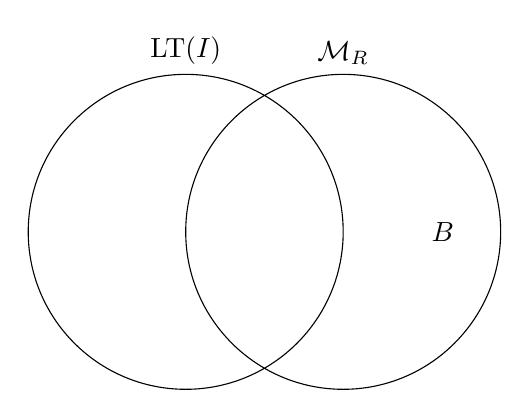
\begin{tikzpicture}
          \draw (-1, 0 ) circle (2)
                (-1, 2 ) node [above] {$\LT(I)$}
                ( 1, 0 ) circle (2)
                ( 1, 2 ) node [above] {$\cal M_R$}
                ( 2, 0 ) node [right] {$B$};
        \end{tikzpicture}
      \end{center}
      
      Either $\LT(f) \in B$ or $\LT(f) \in \LT(I)$.
      In the first case, suppose $\LT(f) = b \in B$.
      Then $f - b \in R - X$ has a smaller leading term than $f$,
      contradicting our choice of $f$.
      Otherwise, suppose $\LT(f) = m \in \LT(I)$.
      Then we can subtract from $f$ any monic polynomial in $I$ with the same leading term,
      again yielding a smaller polynomial in $R - X$.
  \end{description}
\end{proof}
\end{comment}

\begin{corollary}
  \label{cor_dim_R_mod_I}
  $$\dim_K R/I = \#\{ m \in \cal M_R ~|~ m \not\in \LT(I)\}.$$
\end{corollary}
\begin{theorem}
  Let $G = \{g_1, \ldots, g_m\}$ be a Gr\"obner basis and consider the system of polynomial equations
  \[g_1 = \ldots = g_m = 0.\]
  This system has finitely many solutions if and only if for every indeterminate $x_i \in K[x_1, \ldots, x_n]$,
  there is a power $x_i^k$ and element $g \in G$ such that $\LM(g) = x_i^k$.
\end{theorem}
\begin{proof}
  \S 3.6 of \cite{buchberger98}.
\end{proof}

\begin{theorem}
  Let $G = \{g_1, \ldots, g_m\}$ be a Gr\"obner basis and suppose the system of polynomial equations
  \[g_1 = \ldots = g_m = 0\]
  has finitely many solutions.
  Let $N$ be the number of solutions.
  \begin{enumerate}[label=(\roman*)]
    \item $N = \#\{ m \in \cal M_R ~|~ m \not\in \pid{\LT(g_1), \ldots, \LT(g_m)} \}$.
    \item If $I$ is the $R$-ideal generated by $G$, then $N = \dim_K R/I$.
  \end{enumerate}
\end{theorem}
\begin{proof}
  For part (i), see \S 3.6 of \cite{buchberger98}.
  Part (ii) follows from Corollary \ref{cor_dim_R_mod_I}.
\end{proof}
\begin{comment}
\begin{theorem}
  \label{thm_groebner_basis_product}
  Let $I$ and $J$ be ideals of $R = K[x_1, \ldots, x_n]$, generated by Gr\"obner bases, say
  \begin{align*}
    I &= \pid{f_1, \ldots, f_m} \\
    J &= \pid{g_1, \ldots, g_n}.
  \end{align*}
  Then
  \[ \{ f_ig_j ~|~ 1 \leq i \leq m, 1 \leq j \leq n \} \]
  is a Gr\"obner basis for the ideal product $IJ$.
\end{theorem}
\begin{proof}
  \begin{align*}
    \LT(IJ)
      &= \pid{ \LT(h) ~|~ h \in IJ } \\
      &= \pid{ \LT(fg) ~|~ f \in I, g \in J } \\
      &= \pid{ \LT(f)\LT(g) ~|~ f \in I, g \in J } \\
      &= \pid{ \LT(f) ~|~ f \in I } \pid{ \LT(g) ~|~ g \in J } \\
      &= \LT(I) \LT(J) \\
      &= \pid{ \LT(f_i) ~|~ 1 \leq i \leq m } \pid{ \LT(g_j) ~|~ 1 \leq j \leq n } \\
      &= \pid{ \LT(f_i) \LT(g_j) ~|~ 1 \leq i \leq m, 1 \leq j \leq n } \\
      &= \pid{ \LT(f_i g_j) ~|~ 1 \leq i \leq m, 1 \leq j \leq n }
  \end{align*}
\end{proof}
\end{comment}

\begin{theorem}
  \label{thm_groebner_basis_remainder}
  Let $I$ be an ideal of $R$, generated by the Gr\"obner basis $G = \{ g_1, \ldots, g_m \}$. Then,
  \begin{enumerate}[label=(\roman*)]
    \item
    Every polynomial $f \in R$ can be written uniquely in the form
    \begin{equation*}
      f = g + r
    \end{equation*}
    where $g \in I$, $r \in R$, and $r$ is reduced modulo $G$.

    \item
    For any polynomial $f \in R$, $f \in I$ if and only if $r = 0$.
  \end{enumerate}
\end{theorem}
\begin{proof}
  Chapter 2, \S 6, Proposition 1 and Corollary 2 in \cite{cox07}.
\end{proof}

\begin{comment}
It is an obvious fact that, given any polynomial $f \in K[x_1, \ldots, x_n]$,
we can separate $f$ into its homogeneous components.
That is, we can write
\[ f = \sum_{i = 0}^n f_i^* \]
where $n$ is the total degree of $f$ and $f_i^*$ is homogeneous of degree $i$.

Given a point $P = (a_1, \ldots, a_n) \in \bb A_K^n$, we can even write $f$ in the same form,
but where $f_i^*$ is homogeneous in the variables $(x_1 - a_1), \ldots, (x_n - a_n)$.
E.g., in $\bb Q[x,y]$, given the point $P = (1,1)$, 
\[ x^2 + y^2 = [(x - 1)^2 + (y - 1)^2] + [2(x + 1) + 2(y + 1)] + [2]. \]
This is just the multivariate Taylor series expansion of the polynomial around the point $P$.
This generalizes to the following.

\begin{theorem}
  Let $R = K[x_1, \ldots, x_n]$ and let $I$ be an ideal of $R$ given by a Gr\"obner basis $I = \pid{g_1, \ldots, g_m}$.
  Then $f$ can be written uniquely in the form
  \[ f = \sum_{i=0}^t f_i^*, \]
  where $t = \max\{n \in \bb N ~|~ f \in I^n\}$, $f_i^* \in I^i - I^{i+1}$, and $f_i^* \not\in \LT(I^{i+1})$.
\end{theorem}
\begin{proof}
  By Theorem \ref{thm_groebner_basis_product}, our Gr\"obner basis for $I$ gives us a basis for $I^t$.
  Theorem \ref{thm_groebner_basis_remainder} then applies, allowing us to write
  \[ f = f^*_t + r_t \]
  with $f^*_t \in I^t - I^{t+1}$ and $r_t \in R$, $r_t \not\in \LT(I^t)$.
  Applying Theorems \ref{thm_groebner_basis_product} and \ref{thm_groebner_basis_remainder} $t-1$ more times gives the result.
\end{proof}

Essentially, given finitely polynomials $\{ g_i \}$ forming a Gr\"obner basis for an ideal,
we can uniquely perform a homogenous decomposition of any polynomial $f$ with respect to the $g_i$'s.

This also allows us to show that (over a field of sufficiently large characteristic)
$f \in I^2$ if and only if $f$ and its differential $df$ vanish modulo $I$.
\end{comment}



%%%%%%%%%%%%%%%%%%%%%%%%%%%%%%%%%%%%%%%%%%%%%%%%%%
%%%%%                                        %%%%%
%%%%%   Groebner Bases in Coordinate Rings   %%%%%
%%%%%                                        %%%%%
%%%%%%%%%%%%%%%%%%%%%%%%%%%%%%%%%%%%%%%%%%%%%%%%%%

\subsection{Gr\"obner Bases in Coordinate Rings}
\label{sec_groebner_bases_in_coordinate_rings}

While the theory of Gr\"obner bases always takes place in polynomial rings,
the theory may be extended to the coordinate ring of a $C_{3,4}$ curve $C$,
though the equivalence relation leads to a complication.
Take, for example, the ring $K[x,y]$ for some field $K$ with the $C_{3,4}$ monomial order.
Then $x^4 < y^3$ in $K[x,y]$.
Now consider the coordinate ring $K[C] := K[x,y]/\pid{y^3 + x^4 + 1}$
(supposing this curve is non-singular).
This places a relation on $1$, $x^4$, and $y^3$.
How can we compare the monomials $y^3$ and $x^4$ in $K[C]$ if $y^3 \equiv -x^4 - 1$?
Given that $y$ divides $x^4 + 1$ in $K[C]$, is $\pid{y, x^4 + 1}$ a reduced Gr\"obner basis in $K[C]$ or not?
We must therefore make clear what we mean by a Gr\"obner basis in a coordinate ring.

Let $C$ be a $C_{3,4}$ curve given by a polynomial $F$.
Then the ideals of $K[x,y]$ containing $F$ are in bijection with the ideals of $K[C]$
(Theorem III.2.13 in \cite{hungerford}).
Let $G = \pid{g_1, \ldots, g_m}$ be a finite subset of $K[C]$
and let $I = \pid G$ be the $K[C]$-ideal generated by $G$.
Let $\bar f \in K[x,y]$ be the reduction of $f \in R$ modulo $G$,
in the sense of Definition \ref{def_reduced_polynomial},
and treating $G$ as a subset of $K[x,y]$.
We will say that $G$ is a Gr\"obner basis for $I$
if the set $G \cup \{ \bar f \}$ is a Gr\"obner basis in $K[x,y]$ with respect to the $C_{3,4}$ order.

In each of the examples below, let $K = \bb F_{11}$,
and let $C$ be the curve given by $F = y^3 + x^4 + 1 \in K[x,y]$.
\begin{example}
  Consider the ideal $I = \pid{x^2 + x, xy} \subset K[C]$.
  The set $G = \{ x^2 + x, xy \}$ is \emph{not} a Gr\"obner basis for $I$.
  
  The reduction of $F$ modulo $G$ is
  \begin{align*}
    \bar F  &= y^3 + x^4 + 1 \\
            &\equiv y^3 - x^3 + 1 & \text{reduce modulo $x^2 + x$} \\
            &\equiv y^3 + x^2 + 1 & \text{reduce modulo $x^2 + x$} \\
            &\equiv y^3 - x + 1 & \text{reduce modulo $x^2 + x$}.
  \end{align*}
  Now we lift $I$ to $I^* = \pid{x^2 + x, xy, y^3 - x + 1} \subset R$.
  However, one of the $S$-polynomials of the generators of $I^*$ does not reduce to 0 modulo $G$.
  \begin{align*}
    S(x^2 + x, y^3 - x + 1)
      &= (x^2 + x)\frac{x^2y^3}{x^2} - (y^3 - x + 1)\frac{x^2y^3}{y^3} \\
      &= xy^3 + x^3 - x^2 \\
      &\equiv x^3 - x^2 & \text{reduce modulo $xy$} \\
      &\equiv -2x^2 & \text{reduce modulo $x^2 + x$} \\
      &\equiv 2x \pmod G & \text{reduce modulo $x^2 + x$}.
  \end{align*}
  In fact, $I = \pid{x}$ and $\{x\}$ is a Gr\"obner basis in $K[C]$.

  By contrast, $\{x^2 + x, xy\}$ \emph{is} a Gr\"obner basis of $K[x,y]$,
  as per Example \ref{ex_groebner_2}.
\end{example}
\begin{example}
  Consider instead $I = \pid{y^2} \subset K[C]$.
  The reduction of $F$ modulo $y^2$ is $\bar F = x^4 + 1$.
  Lift $I$ to $I^* = \pid{y^2, x^4 + 1} \subset R$.
  There is only one $S$-polynomial to consider on the generators of $I^*$,
  \[ S(y^2, x^4 + 1) = (y^2) \frac{x^4y^2}{y^2} - (x^4 + 1)\frac{x^4y^2}{x^4} = y^2. \]
  This $S$-polynomial reduces to 0 modulo $\{y^2, x^4 + 1\}$,
  hence $\{y^2, x^4 + 1\}$ is a Gr\"obner basis in $K[x,y]$ and $\{y^2\}$ is a Gr\"obner basis in $K[C]$.
  
  This example illustrates the need to compute the reduction $\bar F$ of $F$ modulo $G$,
  since $\{y^2, x^4 + 1\}$ is a Gr\"obner basis in $K[x,y]$, but $\{y^2, y^3 + x^4 + 1\}$ is not.
\end{example}
  
%%%%%%%%%%%%%%%%%%%%%%%%%%%
%%%%%                 %%%%%
%%%%%   Derivations   %%%%%
%%%%%                 %%%%%
%%%%%%%%%%%%%%%%%%%%%%%%%%%

\section{Differential Forms}
\label{chap_differentials}

In a typical undergraduate mathematics curriculum,
derivatives and differential forms appear in the study of real- or complex-valued functions.
In real and complex analysis courses,
it is seen that $\bb R$ and $\bb C$ are complete with respect to their standard metrics.
Concepts such as limits, convergence, and derivatives are defined with respect to these metrics.
In this thesis, we wish to speak of derivatives and differentials of functions that are not real-valued,
but rather members of a polynomial ring $K[x,y]$ over a finite field or a quotient of that polynomial ring.
It is not so clear anymore what is meant by the differential of a polynomial in these discrete spaces.

In this chapter, we define (K\"ahler) differentials of functions purely algebraically
in a sufficient generality as to cover differentials of polynomials in $A = R[x_1, \ldots, x_n]$,
multivariate polynomials with coefficients in a commutative ring with identity $R$.
We will see how to extend this definition to differentials on functions in other spaces constructed from $A$,
such as its field of fractions, quotients, and localizations.
Along the way, we give a natural definition of the formal derivative and formal partial derivative.

The contents of this chapter come mostly from a combination of the books
\cite{eisenbud95}, \cite{eisenbud00}, \cite{goldschmidt03}, and \cite{stichtenoth09}.



%%%%%%%%%%%%%%%%%%%%%%%%%%%
%%%%%                 %%%%%
%%%%%   Derivations   %%%%%
%%%%%                 %%%%%
%%%%%%%%%%%%%%%%%%%%%%%%%%%

\subsection{Derivations}
\begin{definition}
  Let $R$ be a commutative ring, $A$ an $R$-algebra, and $M$ an $A$-module.
  A map $\delta : A \to M$ is called a \defn{derivation} (from $A$ to $M$)
  if it is $R$-linear and satisfies the product rule
  (also called the Leibniz rule):
    \[ \delta(ab) = \delta(a)b + a\delta(b). \]
\end{definition}

Some authors do not require a derivation to be $R$-linear,
and they distinguish between derivations and $R$-linear derivations.
We will assume all derivations are $R$-linear.

As the name suggests, many familiar properties of the derivative from calculus
are an immediate consequence of this definition.
The following are easily verified.
\begin{proposition}
  \label{prop_derivation}
  A derivation satisfies the following properties.
  \begin{enumerate}[label=(\roman*)]
    \item If $A$ is unital, then $\delta(1) = 0$.
    \item If $A$ is unital, then $\delta(r) = 0$ for all $r \in R$.
    \item If $A$ is commutative, then $\delta(x^2) = 2x\delta(x)$.
    \item If $A$ is commutative, then for all integers $n > 0$, $\delta(x^n) = nx^{n-1}\delta(x)$.
    \item If $x$ is a unit, then $\delta(x\inv) = -x^{-2}\delta(x)$.
    \item If $x$ is a unit, then for all $n \in \bb Z$, $\delta(x^n) = nx^{n-1}\delta(x)$.
    \item If $y$ is a unit, then $\delta(xy\inv) = (\delta(x)y - x\delta(y))y^{-2}$.
  \end{enumerate}
\end{proposition}
\begin{comment}
\begin{proof}
  \begin{enumerate}[label=(\roman*)]
    \item
      We have
        \[ D(1) = D(1 \cdot 1) = D(1) \cdot 1 + 1 \cdot D(1) = D(1) + D(1) \]
      which implies $D(1) = 0$.
    \item
      Follows from (i) by $R$-linearity.
    \item
        \[ D(x^2) = D(x)x + xD(x) = xD(x) + xD(x) = 2xD(x). \]
    \item
      Follows from (iii) by induction.
      Suppose $D(x^k) = kx^{k-1}D(x)$ for some $k > 0$. Then
      \begin{align*}
        D(x^{k+1})
          &= D(x^k \cdot x) \\
          &= D(x^k)x + x^kD(x) \\
          &= kx^{k-1}D(x)x + x^kD(x) \\
          &= kx^kD(x) + x^kD(x) \\
          &= (k + 1)x^kD(x).
      \end{align*}
    \item
      By part (i) and the product rule, we have
        \[ 0 = D(1) = D(xx\inv) = D(x)x\inv + xD(x\inv). \]
      This implies
        \[ xD(x\inv) = -D(x)x\inv, \]
      hence
        \[ D(x\inv) = -x^{-2}D(x). \]
    \item
      The case where $n \geq -1$ is handled by parts (i), (iv), and (v).
      The rest follows by induction.
      Suppose $D(x^k) = kx^{k-1}D(x)$ for some $k \leq -1$. Then
      \begin{align*}
        D(x^{k-1})
          &= D(x^kx\inv) \\
          &= D(x^k)x\inv + x^kD(x\inv) \\
          &= kx^{k-1}D(x)x\inv - x^kx^{-2}D(x) \\
          &= kx^{k-2}D(x) - x^{k-2}D(x) \\
          &= (k - 1)x^{k-2}D(x).
      \end{align*}
    \item
      Immediate from the product rule and part (v).
      \begin{align*}
        D(xy\inv)
          &= D(x)y\inv + xD(y\inv) \\
          &= D(x)y\inv - xy^{-2}D(y) \\
          &= (D(x)y - xD(y))y^{-2}.
      \end{align*}
  \end{enumerate}
\end{proof}
\end{comment}

We can define the sum of two derivations $\delta_1$ and $\delta_2$ by
  \[ (\delta_1 + \delta_2)(x) = \delta_1(x) + \delta_2(x) \]
and scalar multiplication of a derivation $\delta$ by a ring element $r$ by
  \[ (r\delta)(x) = r\delta(x). \]
Under these operations, the set of derivations from $A$ to $M$ becomes an $R$-module,
denoted by $\Der_R(A,M)$.
This is the \defn{module of derivations from $A$ to $M$}.
In the case where $M = A$, this may be denoted by $\Der_R(A)$.

Property (v) of Proposition \ref{prop_derivation} shows that if $x$ is a unit,
then $\delta(x\inv)$ is determined by $\delta(x)$.
This suggests that there is a relationship between derivations from an algebra $A$
and derivations from the field of fractions of $A$,
although note that $A$ must not have any zero divisors in order for its field of fractions to be constructed.

\begin{proposition}
  \label{prop_derivation_unique_extension}
  Let $A$ be an $R$-algebra with no zero divisors and let $\delta \in \Der_R(A,M)$.
  Let $B = \Frac A$, the field of fractions of $A$.
  There is a unique $\delta' \in \Der_R(B, M)$ whose restriction to $A$ is $\delta'|_A = \delta$.
\end{proposition}
That is to say that if $\delta$ is a derivation from $A$ to $M$,
it extends uniquely to a derivation from $\Frac A$ to $M$.
\begin{proof}
  If $A = B$, we are done.
  So suppose instead there is a $b \in B$ such that $b\in A$ but $b\inv \not \in A$.
  Suppose $\delta_1, \delta_2 \in \Der_R(B, M)$ are such that $\delta_1|_{A} = \delta = \delta_2|_{A}$.
  Then $\delta_1(b) = \delta(b) = \delta_2(b)$ and
    \[ \delta_1(b\inv) = -b^{-2}\delta_1(b) = -b^{-2}\delta_2(b) = \delta_2(b\inv). \]
  It follows that $\delta_1(ab\inv) = \delta_2(ab\inv)$ for all $ab\inv \in B$.
\end{proof}

In order to understand how a derivation acts on $\Frac A$, it is enough to know how it acts on $A$.
In the case of a derivation over the field $R(x_1, \ldots, x_n)$,
it is enough to know how it acts on the polynomial ring $R[x_1, \ldots, x_n]$.
In the univariate case, we can say even more.
The behaviour of a derivation $\delta: R(x) \to M$ is entirely determined by the value of $\delta(x)$.

\begin{proposition}
  \label{prop_derivation_unique_x}
  Let $R(x)$ be the ring of rational functions over a ring $R$ in a single variable $x$.
  Let $\delta_1, \delta_2 \in \Der_R(R(x))$.
  If $\delta_1(x) = \delta_2(x)$, then $\delta_1 = \delta_2$.
\end{proposition}
\begin{proof}
  For all $r \in R$, we have $\delta_1(r) = \delta_2(r) = 0$.
  For all $f \in R[x]$, we have $\delta_1(f) = \delta_2(f)$ by $R$-linearity.
  Now $\delta_1$ and $\delta_2$ agree on all of $R[x]$.
  By Proposition \ref{prop_derivation_unique_extension}, they must agree on all of $R(x)$.
\end{proof}

For a (unital) ring $R$, the \defn{formal derivative} on $R(x)$
is the unique derivation $D_x \in \Der_R(R(x))$ satisfying $D_x(x) = 1$.
The formal derivative of a function $f$ is often denoted $f' := D_x(f)$,
although this convention will not be adopted here ---
beyond this paragraph, this thesis has no use for derivations on univariate polynomials.
The formal derivative behaves exactly as one might expect.
\begin{example}
  Let $f = 3x^3 + 6x^2 + 1 \in \bb Z[x]$. Then
  \begin{align*}
    D_x(f) 
      &= 3D_x(x^3) + 6D_x(x^2) + D_x(1) & R\text{-linearity} \\
      &= 3 \cdot 3 x^2 D_x(x) + 6 \cdot 2 x D_x(x) + 0 & \text{Proposition \ref{prop_derivation}}\\
      &= 9 x^2 + 12 x & D_x(x) = 1.
  \end{align*}
\end{example}

\begin{comment}
Up to this point, we have discussed derivations without showing that such a thing even exists.
The following proposition establishes the existence of derivations by exhibiting one that should be familiar.

\begin{proposition}
  \label{prop_derivation_formal_derivative}
  Let $R(x)$ be the ring of rational functions over a ring $R$ in a single variable $x$.
  There is a unique derivation $D_x : R(x) \to R(x)$ satisfying $D_x(x) = 1$.
\end{proposition}
Given a rational function $f(x)$, the function $D_x(f(x))$ is the \defn{formal derivative} of $f(x)$, often written $f'(x)$.
\begin{proof}
  We need only show existence of a derivation on $R[x]$ with the desired property.
  By propositions \ref{prop_derivation_unique_extension} and \ref{prop_derivation_unique_x},
  this derivation is unique and extends uniquely to a derivation on $R(x)$ with the desired property.
  
  We set $D_x(x) = 1$ and extend by linearity to get its action on all of $R[x]$.
  If $f(x) = \sum f_ix^i \in R[x]$, then
    \[ D(f(x)) = \sum if_ix^{i-1}D(x) = \sum if_ix^{i-1}. \]
  We must show that this satisfies the product rule.
  Let $g(x) = \sum g_jx^j$. Then for all $f(x), g(x) \in R[x]$,
  
  \begin{align*}
    D_x(f(x)g(x))
      &= D_x \left( \left( \sum_{i=0}^m f_ix^i \right) \left( \sum_{j=0}^n g_jx^j \right) \right) \\
      &= D_x \left( \sum_{i=0}^m \sum_{j=0}^n f_ix^i g_jx^j \right) \\
      &= D_x \left( \sum_{i=0}^m \sum_{j=0}^n f_ig_jx^{i+j} \right) \\
      &= \sum_{i=0}^m \sum_{j=0}^n f_ig_jD_x(x^{i+j}) \\
      &= \sum_{i=0}^m \sum_{j=0}^n (i+j)f_ig_jx^{i+j-1} \\
      &= \sum_{i=0}^m \sum_{j=0}^n (if_ig_jx^{i+j-1} + jf_ig_jx^{i+j-1}) \\
      &= \sum_{i=0}^m \sum_{j=0}^n if_ig_jx^{i+j-1} + \sum_{i=0}^m \sum_{j=0}^n jf_ig_jx^{i+j-1} \\
      &= \left( \sum_{i=0}^m if_ix^{i-1} \right) \left( \sum_{j=0}^n g_jx^j \right) + \left( \sum_{i=0}^m f_ix^i \right) \left( \sum_{j=0}^n jg_jx^{j-1} \right) \\
      &= D_x(f(x)) g(x) + f(x)D(g(x)).
  \end{align*}
\end{proof}
\end{comment}

Now consider the $R$-algebra $A = R(x_1, \ldots, x_n)$, rational functions in $n$ variables.
For each $1 \leq i \leq r$,
we can set $S_i = R(x_1, \ldots, x_{i-1}, x_{i+1}, \ldots, x_n)$, so that $A = S_i(x_i)$.
We have merely realized $A$ as the algebra of rational functions in one variable $x_i$ and coefficients in $S_i$,
which is the algebra of rational functions in the other $n - 1$ variables.
Then Proposition \ref{prop_derivation_unique_x} says that
there is a unique derivation $D_{x_i} \in \Der_{S_i}(A)$ satisfying $D_{x_i}(x_i) = 1$.
This derivation $D_{x_i}$ is also a member of $\Der_R(A)$ and its action on the other indeterminates of $A$ is
\begin{align*}
  D_{x_i}(x_j) &= \begin{cases} 1 & i = j \\ 0 & i \neq j \end{cases}.
\end{align*}
The requirement that $D_{x_i}(x_j) = 0$ when $i \neq j$ is a consequence of $S_i$-linearity
by $D_{x_i}$'s membership in $\Der_{S_i}(A)$.
If $f \in A$, then $f_{x_i} := D_{x_i}(f)$ is the \defn{formal partial derivative} with respect to $x_i$.

\begin{example}
  In the case of $A = \bb Z[x,y]$, we have derivations $D_x$ and $D_y$ with
  $D_x(x) = 1 = D_y(y)$ and $D_x(y) = 0 = D_y(x)$.
  Let $f = x^2 + xy + y^3 \in A$.
  Then $f_x = D_x(f) = 2x + y$ and $f_y = D_y(f) = x + 3y^2$.
\end{example}

\begin{comment}
\begin{proposition}
  Let $D \in \Der_K(A)$ be a derivation.
  Let $I$ be an ideal of $A$.
  Then $D$ induces a derivation $D^* \in \Der_K(A/I)$ defined by
    \[ D^*([a]) = [D(a)]. \]
\end{proposition}
\begin{proof}
  For each $a \in A$, denote the equivalence class containing $a$ in $A/I$ by $\bar a$.
  We show first that this map is well-defined.
  Suppose $\bar a = \bar b$.
  Then $\bar{a-b} = \bar 0$ and
    \[ D^*(\bar a) = D^*(\bar a - \bar{a-b}) = D^*(\bar{a-a+b}) = D^*(\bar b). \]
  We must also show that $D^*(\bar k \cdot \bar a) = \bar k \cdot D^*(\bar a)$
  and $D^*(\bar a \cdot \bar b) = D^*(\bar a) \cdot \bar b + \bar a \cdot D^*(\bar b)$.
    \[ D^*(\bar k \cdot \bar a) = D^*(\bar{ka}) = \bar{D(ka)} = \bar{kD(a)} = \bar k \cdot \bar{D(a)} = \bar k \cdot D^*(\bar a) \]
  \begin{align*}
    D^*(\bar a \cdot \bar b)
      &= D^*(\bar{ab})
       = \bar{D(ab)}
       = \bar{D(a)b + aD(b)} \\
       &= \bar{D(a)} \cdot \bar b + \bar a \cdot \bar{D(b)}
       = D^*(\bar a) \cdot \bar b + \bar a \cdot D^*(\bar b)
  \end{align*}
\end{proof}
With this we can extend formal derivatives of functions in $K[x,y]$ and $K(x,y)$ to formal derivatives of functions in $K[C]$ and $K(C)$.
\end{comment}

We may compose derivations with a morphisms of algebras to obtain new derivations.

\begin{proposition}
  \label{prop_precompose_derivation}
  Let $f \in \Hom_R(A,B)$ be a morphism of $R$-algebras and let $\delta \in \Der_R(B,M)$ be an $R$-linear derivation.
  \[ \begin{tikzcd} A \arrow{r}{f} & B \arrow{r}{\delta} & M \end{tikzcd} \]
  Then $\delta \circ f \in \Der_R(A,M)$.
\end{proposition}
\begin{proof}
  While $M$ is a $B$-module, it becomes an $A$-module under the $A$-action
    \[ A \times M \to M : (a, m) \mapsto f(a)m. \]
  Both $f$ and $\delta$ are $R$-linear, so $\delta \circ f$ is also $R$-linear.
  As for the product rule, let $a, b \in A$. Then
  \begin{align*}
    (\delta \circ f)(ab)
      &= \delta(f(ab)) \\
      &= \delta(f(a)f(b)) \\
      &= \delta(f(a))f(b) + f(a)\delta(f(b)) \\
      &= (\delta \circ f(a))f(b) + f(a)(\delta \circ f(b)) \\
      &= (b, \delta \circ f(a)) + (a, \delta \circ f(b)). \qedhere
  \end{align*}
\end{proof}



%%%%%%%%%%%%%%%%%%%%%%%%%%%%%%%%%%%%
%%%%%                          %%%%%
%%%%%   Universal Derivation   %%%%%
%%%%%                          %%%%%
%%%%%%%%%%%%%%%%%%%%%%%%%%%%%%%%%%%%

\subsection{K\"ahler Differentials}
\label{sec_kahler_differentials}

In this section, we briefly present a construction of K\"ahler differentials and some important properties.
For more detail, as well as alternative constructions,
see \cite{eisenbud95}, \cite{eisenbud00}, \cite{goldschmidt03}, or \cite{stichtenoth09}.

Let $A$ be an $R$-algebra.
The \defn{module of K\"ahler differentials} of $A$ over $R$,
denoted by $\Omega_{A/R}$,
is the $A$-module generated by the set $\{ d(a) ~|~ a \in A \}$,
where $d(a)$ is merely a symbol,
modulo the relations
\begin{align*}
  d(ab) &= d(a)b + ad(b) \\
  d(ra + sb) &= rd(a) + sd(b)
\end{align*}
for all $r, s \in R$ and $a, b \in A$.
The elements of $\Omega_{A/R}$ are called \defn{differential forms} or \defn{K\"ahler differentials}.
We will write $d(a)$ as simply $da$, though we will not write $d(ab)$ as $dab$, as this may be confused with $d(a)b$.
The map
  \[ d_A : A \to \Omega_{A/R} : a \mapsto d(a) \]
is an $R$-linear derivation, called the \defn{universal derivation}.
It is universal in the following sense.
If $\delta : A \to M$ is another $R$-linear derivation from $A$,
then there is a unique morphism of $R$-modules $\phi : \Omega_{A/R} \to M$ such that
\[ \begin{tikzcd}
  A \arrow{r}{d_A} \arrow[swap]{dr}{\delta} & \Omega_{A/R} \arrow[dashed]{d}{!\exists \phi} \\ & M
\end{tikzcd} \]
commutes.
This map is defined by $\phi : da \mapsto \delta(a)$.
We will omit the subscript and write $d$ in place of $d_A$,
except in contexts where there are multiple $d$'s and we need to distinguish them by their domains.

\begin{comment}
\begin{proposition}
  A morphism $\phi : A \to B$ of $R$-algebras induces
  a morphism $\psi : \Omega_{A/R} \to \Omega_{B/R}$ of $A$-modules.
\end{proposition}
\begin{proof}
  Let $\phi : A \to B$ be a morphism of $R$-algebras.
  We have the following maps,
  \[ \begin{tikzcd}
      A \arrow{r}{d_A} \arrow[swap]{d}{\phi} & \Omega_{A/R} \\ B \arrow[swap]{r}{d_B} & \Omega_{B/R}.
    \end{tikzcd} \]
  By Proposition \ref{prop_precompose_derivation},
  the composition $d_B \circ \phi : A \to \Omega_{B/R}$ is an $R$-linear derivation.
  By the universal property of the universal derivation,
  there is a unique map $\psi : \Omega_{A/R} \to \Omega_{B/R}$ such that
  \[ \begin{tikzcd}
      A \arrow{r}{d_A} \arrow[swap]{dr}{d_B \circ \phi} & \Omega_{A/R} \arrow[dashed]{d}{\psi} \\ & \Omega_{B/R}
    \end{tikzcd} \]
  commutes.
\end{proof}
The induced map sends $d_Aa \mapsto d_B(\phi(a))$.
\end{comment}

Of particular interest to us in this thesis is the case where $A = R[x_1, \ldots, x_n]$ is a polynomial ring.
In this case, $\Omega_{A/R}$ is the free $A$-module generated by the symbols $dx_1, \ldots, dx_n$.
\begin{proposition}
  \label{prop_differential_module_of_polynomial_ring}
  Let $A = R[x_1, \ldots, x_n]$. Then
  \[ \Omega_{A/R} \cong \bigoplus_{i=1}^n Adx_i. \]
\end{proposition}
\begin{comment}
\begin{corollary}
  Let $A = R[x_1, \ldots, x_n]$, let $I$ be an ideal of $A$, and let $B = A/I$.
  Then $B$ is an $R$-algebra and
  \[ B \otimes_{R} \Omega_{A/R} \cong \bigoplus_{i=1}^n Bdx_i. \]
\end{corollary}
\begin{proof}
  \note{Extension of scalars.}
\end{proof}
Here $\otimes_R$ denotes the tensor product of algebra.
We will use this corollary in Chapter \ref{chap_curves}, after defining the coordinate ring of a curve,
when relating differentials forms of a polynomial ring to those of a coordinate ring.
Since $\Omega_{A/R}$ is a direct sum of $R$-algebras $Adx_i$,
there is a family of natural projection maps 
  \[ \pi_i : \Omega_{A/R} \to Adx_i : \sum f_jdx_j \mapsto f_idx_i. \]
We can compose the maps
  \[ \begin{tikzcd}
    A \arrow{r}{d} & \Omega_{A/R} \arrow{r}{\pi_i} & Adx_i \arrow{r}{} & A
  \end{tikzcd} \]
where the right-most map sends $dx_i \mapsto 1$.
The composition of the three maps is the formal partial derivative with respect to $x_i$.
\end{comment}



%%%%%%%%%%%%%%%%%%%%%%%%%%%%%%%%%%%%%%%%%%
%%%%%                                %%%%%
%%%%%   Differential Forms in K[C]   %%%%%
%%%%%                                %%%%%
%%%%%%%%%%%%%%%%%%%%%%%%%%%%%%%%%%%%%%%%%%

\subsection{Differential Forms in $K[C]$}
\label{sec_differentials_in_coordinate_ring}

In Section \ref{sec_kahler_differentials}, we defined $\Omega_{A/R}$,
the module of K\"ahler differentials on an $R$-algebra $A$.
The coordinate ring is a $K$-algebra, so let us describe the structure of $\Omega_{K[C]/K}$.
To do so, we will make use of the following proposition.

\begin{proposition}
  \label{prop_conormal_sequence}
  Let $\pi : A \to B$ be an epimorphism of $R$-algebras.
  Let $I = \ker \pi$.
  There is an exact sequence of $B$-modules
    \[ I/I^2 \xrightarrow{d} B \tensor A \Omega_{A/R} \xrightarrow{D\pi} \Omega_{B/R} \to 0 \]
  where $d : [f] \mapsto 1 \otimes df$ and $D\pi : b \otimes da \mapsto b(da)$.
\end{proposition}
\begin{proof}
  Proposition 16.3 in \cite{eisenbud95}.
\end{proof}

This proposition makes use of the tensor product of modules.
The tensor product will not be defined or discussed in this thesis;
one may consult \cite{dummit04}, \cite{eisenbud95}, or \cite{hungerford} for more on that topic.
We will take advantage of other results to turn the tensor product into a direct sum of modules.

To understand the structure of $\Omega_{K[C]/K}$,
we begin by noting that the canonical quotient map $q : K[x,y] \to K[C]$ is an epimorphism of $K$-algebras
whose kernel is $\ker q = \pid F$, the ideal of $K[x,y]$ generated by the defining polynomial of the curve.
Proposition \ref{prop_conormal_sequence} therefore applies, telling us that there is an exact sequence
\begin{center}
\begin{tikzcd}
  \frac{\pid{F}}{\pid{F^2}} \arrow{r}{d} &
  K[C] \tensor {K[x,y]} \Omega_{K[x,y]/K} \arrow{r}{Dq} &
  \Omega_{K[C]/K} \arrow{r}{} &
  0.
\end{tikzcd}
\end{center}
Using a property of exact sequences (see remarks on page 176 of \cite{hungerford}), 
\[ \Omega_{K[C]/K} \cong \frac {K[C] \tensor {K[x,y]} \Omega_{K[x,y]/K}} {\im d}. \]
Next applying Proposition \ref{prop_differential_module_of_polynomial_ring},
\[ \Omega_{K[C]/K} \cong \frac {K[C] \tensor {K[x,y]} \Omega_{K[x,y]/K}} {\im d}
                   \cong \frac {K[C] \tensor {K[x,y]} (K[x,y]dx \oplus K[x,y]dy)} {\im d}. \]
The tensor product distributes over addition (Theorem IV.5.9 \cite{hungerford}), giving
\[ \Omega_{K[C]/K} \cong \frac {\left(K[C] \tensor {K[x,y]} K[x,y]dx\right) \oplus
                                \left(K[C] \tensor {K[x,y]} K[x,y]dy\right)} {\im d}. \]
A basic property of the tensor product is that an $R$-module $A$ tensored with its ring $R$ is isomorphic to itself,
i.e. $A \tensor R R \cong A$ (Theorem IV.5.7 \cite{hungerford}), hence
\[ \Omega_{K[C]/K} \cong \frac {K[C]dx \oplus K[C]dy} {\im d}. \]

To determine the image of $d$, it is enough to know the image of the element $F \in \pid F / \pid{F^2}$.
The element $F \in \pid F / \pid{F^2}$ maps to $1 \otimes dF \in K[C] \otimes \Omega_{K[x,y]/K}$.
Following the chain of isomorphisms we just produced, this then maps to $F_xdx + F_ydy \in K[C]dx \oplus K[C]dy$.
Thus,
\[ \Omega_{K[C]/K} \cong \frac {K[C]dx \oplus K[C]dy} {\pid{F_xdx + F_ydy}}. \]
The module $\Omega_{K[C]/K}$ of differentials on $K[C]$ is generated by $dx$ and $dy$,
modulo the equivalence relation $F_xdx \equiv -Fydy$.
This relation between $dx$ and $dy$ means that it is therefore a rank 1 $K[C]$-module, generated by a single element.
\begin{proposition}
  \label{prop_differential_generator}
  There is a generator $dz$ for $\Omega_{K[C]/K}$ with the properties
  \begin{align*}
    dx &\equiv F_ydz \\
    dy &\equiv -F_xdz.
  \end{align*}
\end{proposition}
\begin{proof}
  See Lemma 5.1 in \cite{salem07}.
\end{proof}
In fact, there are many possible generators for $\Omega_{K[C]/K}$.
Another choice of generator allowing for more efficient doubling of typical divisors
will be presented in Chapter \ref{chap_doubling}.
The generator in Proposition \ref{prop_differential_generator} is a natural choice
that is useful for some proofs, and will be used in some atypical cases of divisor doubling.

The differential of a function $f \in K[C]$ with respect to this generator $dz$ is
\[ df = (f_xF_y - f_yF_x)dz. \]
If $I$ is an ideal of $K[C]$,
we will say by abuse of notation that $df \in I$ if $f_xF_y - f_yF_x \in I$.
Equivalently, we will say that $df \in I$ if $df$ vanishes modulo $I$.

Now let $\cal O_{\frak p}$ be the local ring at a prime ideal $\frak p$ of $K[C]$.
Then there is a map $d_{\cal O_{\frak p}} : \cal O_{\frak p} \to \Omega_{\cal O_{\frak p}/K}$.
The action of this map is inherited from the map $d_{K[C]} : K[C] \to \Omega_{K[C]/K}$.
That is, the differential of a function $f/g \in \cal O_{\frak p}$ is
\[ d_{\cal O_{\frak p}} \left( \frac f g \right) = \frac{d_{K[C]}(f)g - fd_{K[C]}(g)}{g^2}
 = \frac{(f_xC_y - f_yC_x)g - f(g_xC_y - g_yC_x)}{g^2} dz . \]
As noted earlier in this chapter, for readability, we will omit the subscripts on $d$
when it is clear in context which differential map is meant.

\begin{lemma}
  \label{lem_differential_of_uniformizer}
  Let $\frak p$ be a non-zero prime ideal of $\bar K[C]$.
  Let $u$ be a uniformizer for $\frak m_{\frak p}$, the maximal ideal of $\cal O_{\frak p}$.
  Then $du \not \in \frak m_{\frak p}$.
\end{lemma}
\begin{proof}
  Let $\frak p = \pid{x - x_0, y - y_0}$.
  Since $C$ is non-singular, the partial derivatives of $C$ are not simultaneously zero at $P = (x_0, y_0)$,
  so suppose without loss of generality that $C_y(x_0, y_0) \neq 0$.
  Then the tangent line to $C$ at $P$ is non-vertical and $u = x - x_0$ is a uniformizer for $\frak m_{\frak p}$.
  Then $du = dx = C_y \not\in \frak m_{\frak p}$.
\end{proof}
\begin{theorem}
  \label{thm_differential_increases_order}
  Let $\frak p$ be a non-zero prime ideal of $K[C]$ and $f$ a polynomial in $K[C]$.
  Suppose $\nu_{\frak p}(f) \geq n$ for some non-negative integer $n$. Then
  \[ \nu_{\frak p}(f) \geq n + 1 \iff \nu_{\frak p}(df) \geq n. \]
\end{theorem}
\begin{proof}
%\frak m_{\frak p}
  Let $u$ be a uniformizer for $\frak m_{\frak p}$.
  Then $f = au^n$ for some $a \in K(C)^*$, and
  \[ df = d(au^n) = u^nda + nau^{n-1}du. \]
  Now $u^nda \in \frak m_{\frak p}^n$,
  so $df \in \frak m_{\frak p}^n$ if and only if $nau^{n-1}du \in \frak m_{\frak p}^n$.
  But $n, du \not\in \frak m_{\frak p}$,
  so this is true if and only if $au^{n-1} \in \frak m_{\frak p}^n$. Hence
  \[ df \in \frak m_{\frak p}^n
    \iff au^{n-1} \in \frak m_{\frak p}^n
    \iff au^n \in \frak m_{\frak p}^{n+1}
    \iff f \in \frak m_{\frak p}^{n+1}. \qedhere \]
\end{proof}
\begin{comment}
\begin{theorem}
  Let $A = K[x_1, \ldots, x_n]$ and let $I$ be an ideal of $A$.
  If $f \in I^2$, then $f \equiv 0$ and $df \equiv 0$ modulo $I$.
\end{theorem}
\begin{proof}
  Let $f \in I^2$.
  Then $f \in I$, so $f \equiv 0 \pmod I$.
  As for its differential, we have that $f$ is generated by a Gr\"obner basis {$g_i$}
  \[ f = \sum a_{i,j}g_ig_j, \]
  so
  \begin{align*}
    df &= d \left( \sum_{\substack{1 \leq i \leq j \leq m}} a_{i,j}g_ig_j \right) \\
       &= \sum_{\substack{1 \leq i \leq j \leq m}} d \left( a_{i,j}g_ig_j \right) \\
       &= \sum_{\substack{1 \leq i \leq j \leq m}} \left( d(a_{i,j})g_ig_j + a_{i,j}d(g_i)g_j + a_{i,j}g_id(g_j) \right) \\
       &\equiv 0 \pmod I
  \end{align*}
\end{proof}

The converse is not true in general.
A simple counterexample is to let $A = \bb F_2[x]$, let $f = x^2$, and let $I = \pid f$.
Then $f \equiv 0 \pmod I$ and $df = 2xdx \equiv 0 \pmod I$.
However, $f \not\in I^2 = \pid{x^4}$.

It is true under additional assumptions.

\begin{theorem}
  Let $A = K[x_1, \ldots, x_n]$ and let $I$ be an ideal of $A$.
  Let $f \in A$ be a polynomial whose formal partial derivatives do not all vanish.
  If $f, df \equiv 0 \pmod I$, then $f \in I^2$.
\end{theorem}
\begin{proof}
  We prove the contrapositive.
  Suppose $f \not\in I^2$.
  If $f \not\equiv 0 \pmod I$, we are done, so suppose $f \equiv 0 \pmod I$ (i.e. $f \in I$).
  We wish to show that $df \not\equiv 0 \pmod I$.

  By Theorem \ref{thm_groebner_basis_remainder}, we can write $f$ as
  \[ f = g + r \]
  where $g \in I^2$ and $r \not\in \LT(I^2)$. Furthermore, $0 \neq r \in I$.
  Since $r \not\in \LT(I^2)$, $D_{x_k}(r) \not\in \LT(I^2)$ for any $1 \leq k \leq n$.
  \begin{align*}
    df &= dg + dr \\
       &\equiv dr \pmod I \\
       &= \sum D_{x_i}(r)dx_i
  \end{align*}
  We must argue now that for each summand $D_{x_i}(r)dx_i$ is non-zero modulo $I$.
  
  Suppose that $D_{x_k}(r) \equiv 0$ for some $1 \leq k \leq n$.
  \begin{align*}
    & D_{x_k}(r) \equiv 0 \pmod I \\
    \implies & D_{x_k}(r) \in I \\
    \implies & \LT(D_{x_k}(r)) \in \LT(I) \\
    \implies & \LT(D_{x_k}(r)) \in \LT(I)\LT(I) \\
    \implies & \LT(D_{x_k}(r)) \in \LT(I^2).
  \end{align*}
  However, as noted earlier, no term in $D_{x_k}(r)$ is in $\LT(I^2)$.
  \note{(Wording.)}
\end{proof}

\begin{proof}
  We prove the contrapositive.
  Suppose $f \not\in I^2$.
  If $f \not\equiv 0 \pmod I$, we are done, so suppose $f \equiv 0 \pmod I$ (i.e. $f \in I$).
  We wish to show that $df \not\equiv 0 \pmod I$.

  By Theorem \ref{thm_groebner_basis_remainder}, we can write $f$ as
  \[ f = g + r \]
  where $g \in I^2$ and $r \not\in \LT(I^2)$.
  Taking the differential of $f$,
  \begin{align*}
    df &= \sum_{i=1}^n D_{x_i}(f)dx_i.% \\
%       &= \sum_{i=1}^n D_{x_i}(g + r)dx_i \\
  \end{align*}
  We must show that one of $df$'s summands is non-zero modulo $I$.
  Since $f$ has a non-zero formal partial derivative, let $k$ be such that $D_{x_k}(f) \neq 0$.
  Then
  \begin{align*}
    D_{x_k}(f)
      &= D_{x_k}(g + r) \\
      &= D_{x_k}(g) + D_{x_k}(r) \\
      &\equiv D_{x_k}(r) \pmod I.
  \end{align*}
  Now suppose $D_{x_k}(r) \equiv 0 \pmod I$. Then
  \begin{align*}
    & D_{x_k}(r) \equiv 0 \pmod I \\
    \implies & D_{x_k}(r) \in I \\
    \implies & \LT(D_{x_k}(r)) \in \LT(I) \\
    \implies & \LT(D_{x_k}(r)) \in \LT(I)\LT(I) \\
    \implies & \LT(D_{x_k}(r)) \in \LT(I^2).
  \end{align*}
  %However, as noted earlier, no term in $D_{x_k}(r)$ is in $\LT(I^2)$.
  %\note{(Wording.)}
\end{proof}

\begin{proof}
  \note{(Supposing $I = \sqrt I$.)}
  We prove the contrapositive.
  Suppose $f \not\in I^2$.
  If $f \not\equiv 0 \pmod I$, we are done, so suppose $f \equiv 0 \pmod I$ (i.e. $f \in I$).
  We wish to show that $df \not\equiv 0 \pmod I$.

  By Theorem \ref{thm_groebner_basis_remainder}, we can write $f$ as
  \[ f = g + r \]
  where $g \in I^2$ and $r \not\in \LT(I^2)$.
  Taking the differential of $f$,
  \begin{align*}
    df &= dg + dr \\
       &\equiv dr \pmod I \\
       &= d\left(\sum_{i=1}^m a_ig_i \right) \\
       &\equiv \sum_{i=1}^m a_id(g_i) \pmod I.
  \end{align*}
\end{proof}



\begin{theorem}
  Let $\frak p$ be a prime ideal of $K[C]$.
  Let $f \in \frak p$.
  Then $f \in \frak p^2$ if and only if $df \in \frak p$.
\end{theorem}
\begin{proof}
  Let $r = \ord_{\frak p}f$. 
  Then $f$ may be written
  \[ f = \sum_{i=1}^r a_iu^i,\]
  where $u$ is a uniformizer of $\frak m_{\frak p}$ and $a_i \not\in \frak m_{\frak p}$. Then
  \begin{align*}
    df &= \sum_{i=1}^r d(a_iu^i) \\
       &= \sum_{i=1}^r (u^ida_i + a_id(u^i)) \\
       &= \sum_{i=1}^r (u^ida_i + ia_iu^{i-1}du) \\
       &= \sum_{i=1}^r u^ida_i + \sum_{i=0}^{r-1} (i+1)a_{i+1}u^idu.
  \end{align*}
  Now $df \in \frak p$ if and only if the $i=0$ term in the second sum is zero,
  i.e. if and only $a_1du = 0$.
  However, since $du \neq 0$, we have
  \[ df \in \frak p \iff a_1 = 0 \iff f \in \frak p^2. \]
\end{proof}
\end{comment}

%%%%%%%%%%%%%%%%%%%%%%%%%
%%%%%              %%%%%
%%%%%   Divisors   %%%%%
%%%%%              %%%%%
%%%%%%%%%%%%%%%%%%%%%%%%

\section{Divisors}
\subsection{The Divisor Class Group}

Let $C$ be a non-singular, projective curve over a field $K$.
The \defn{group of divisors} on $C$, denoted by $\Div_{\bar K}(C)$, is the free Abelian group generated by the points of $C(\bar K)$.
A \defn{divisor} of $C$ is any element of this group; it is a finite formal sum of points.
If $P$, $Q$, and $R$ are points on the curve $C$, then examples of divisors include
  \[ \begin{array}{c} P + Q + R \\ P + 3Q - 2R \\ Q \\ 0 \end{array}. \]

If $D$ is a divisor and $P$ is a point on $C$, the \defn{order} of $D$ at $P$, denoted by $\ord_P(D)$, is the coefficient of $P$ in this sum.
For example, if $D = P + 3Q - 2R$, then $\ord_Q(D) = 3$ and $\ord_R(D) = -2$.
A divisor $D$ is called \defn{effective} if $\ord_P(D) \geq 0$ at every point $P$.
So $P + Q + R$, $Q$, and $0$ are effective divisors, while $P + 3Q - 2R$ is not.

The degree of a divisor, denoted by $\deg(D)$, is the sum of the orders of $D$ at all points,
  \[ \deg(D) = \sum_{P \in C}\ord_P(D). \]
For instance, $\deg(P + 3Q - 2R) = 2$.
If $D$ and $D'$ are both divisors of $C$, then $\deg(D + D') = \deg(D) + \deg(D')$.
Consequently, divisors with degree zero form a subgroup $\Div_{\bar K}^0(C)$ of $\Div_{\bar K}(C)$.

If $L$ is an algebraic extension of $K$ and $\sigma \in \Gal(\bar K/L)$,
then $\sigma$ extends an action on points of $C(L)$, via
  \[ \sigma(x : y : z) = (\sigma(x) : \sigma(y) : \sigma(z)). \]
This, in turn, extends to an action on $\Div_{\bar K}(C)$.
If $D$ is the divisor
  \[ D = \sum_{P \in C(\bar K)} n_P P, \]
then define
  \[ \sigma(D) = \sum_{P \in C(\bar K)} n_P \sigma(P). \]
A divisor $D$ is \defn{defined over $L$} if $\sigma(D) = D$ for all $\sigma \in \Gal(\bar K/L)$.
That is, if $D$ remains fixed by every embedding of $L$ in $\bar K$.
The set of divisors on $C$ defined over $L$ is denoted by $\Div_L(C)$.
The set $\Div_L(C)$ forms a subgroup of $\Div_{\bar K}(C)$, and $\Div_L^0(C)$ a subgroup of both $\Div_L(C)$ and $\Div_{\bar K}^0(C)$.

This last definition deserves a few examples.
\begin{example}
  Let $K$ be any field, $L$ any algebraic extension and $\sigma \in \Gal(\bar K/L)$.
  By definition, $\sigma$ fixes $L$.
  If $P$ is any point with coordinates in $L$, then $\sigma(P) = P$.
  If $D$ is any divisor consisting only of points with coordinates in $L$, then $\sigma(D) = D$ and $D$ is defined over $L$.
\end{example}
\begin{example}
  Let $K = \bb F_2$ and let $L = K(\alpha)$ be an algebraic extension with $\alpha^2 + \alpha = 1$.
  Let $C$ be the curve $x^4 + y^3 + x + 1$ over $K$.
  Let $P$ be the point $(\alpha : 1 : 1)$ on $C$ and let $D$ be the divisor $D = P$.
  There is an automorphism $\sigma \in \Gal(\bar K/K)$ that maps $\alpha \mapsto \alpha + 1$, so 
    \[ \sigma(D) = \sigma(P) = (\sigma(\alpha) : \sigma(1) : \sigma(1)) = (\alpha + 1 : 1 : 1) \neq D. \]
  Hence $D$ is not defined over $K$.
\end{example}
\begin{example}
  Let $K$, $L$, $C$, and $P$ be as in the previous example.
  Let $Q = (\alpha + 1 : 1 : 1)$, which is also a point on $C$.
  Let $D$ be the divisor $D = P + Q$.
  Every automorphism $\sigma$ in $\Gal(\bar K/K)$ maps either $\alpha$ to itself or to $\alpha + 1$.
  In the former case,
  \begin{align*}
    \sigma(D) &= \sigma(P) + \sigma(Q) \\
              &= (\sigma(\alpha) : \sigma(1) : \sigma(1)) + (\sigma(\alpha + 1) : \sigma(1) : \sigma(1)) \\
              &= (\alpha : 1 : 1) + (\alpha + 1 : 1 : 1) \\
              &= P + Q = D.
  \end{align*}
  In the latter case,
  \begin{align*}
    \sigma(D) &= \sigma(P) + \sigma(Q) \\
              &= (\sigma(\alpha) : \sigma(1) : \sigma(1)) + (\sigma(\alpha + 1) : \sigma(1) : \sigma(1)) \\
              &= (\alpha + 1 : 1 : 1) + (\alpha : 1 : 1) \\
              &= Q + P = D.
  \end{align*}
  So $D$ is defined over $K$.
\end{example}

A divisor, being a formal sum of points, can be used to record the zeroes and poles of a function.
Let $f \in K(C)$ be a rational function.
The \defn{divisor of $f$} is
  \[ \div f := \sum_{P \in C(\bar K)} v_P(f)P, \]
where $v_P(f)$ is the valuation of $f$ at $P$ (with respect to the curve $C$).
Recall \note{(from an earlier section)} that $v_P(f)$ is the multiplicity of the intersection of $f$ and $C$ at $P$.
\note{(What if $v_P(f) < 0$?)}
If $D$ is the divisor of some rational function, then $D$ is called a \defn{principal divisor}.
In the following, we will see that principal divisors form a subgroup of degree zero divisors.

\begin{proposition}
  Let $k \in K^*$ and let $f, g \in K(C)^*$. Then
  \begin{enumerate}[label=(\roman*)]
    \item $\div(k) = 0$;
    \item $\div(fg) = \div f + \div g$.
  \end{enumerate}
\end{proposition}
\begin{proof}
  \note{TODO}
\end{proof}
\begin{theorem}
  Let $C$ be a curve over $K$ and let $f \in K(C)^*$.
  Then $f$ has finitely many zeroes and poles and $\deg(\div f) = 0$.
\end{theorem}
\begin{proof}
  Galbraith Thm 8.3.14.
\end{proof}

These theorems combined show that the principal divisors are a subset of the degree zero divisors and remain closed as a group.
They therefore form a (normal) subgroup of $\Div_{\bar K}^0(C)$.
The group of principal divisors on $C$ (defined over $K$) is denoted by $\Princ_K(C)$.

At last we arrive at defining the divisor class group.
The \defn{divisor class group} is the quotient group,
  \[ \Jac_K^0(C) = \frac{\Div_K^0(C)}{\Princ_K(C)}. \]
The divisor class group of $C$ is also called the \defn{Jacobian} of $C$ or the \defn{Picard group} of $C$.
It is sometimes denoted by $\Pic_K^0(C)$.

\begin{itemize}
  \item Every divisor equivalent to one of the form $P_1 + \dots + P_n - nP_\infty$.
        (For any term of the form $-mP$, add $m \div f$ for any polynomial $f$ through $P$.)
  \item Riemann Roch Theorem implies divisor equivalent to one with $n \leq g$. (How?)
        Such a divisor is called reduced. (Is it unique?)
\end{itemize}

Operations with divisors.
\begin{itemize}
  \item Addition
  \item Negation
  \item LCM
  \item GCD
\end{itemize}



\subsection{The Ideal Class Group}

Given the point set of a curve, we were able to construct the divisor class group of the curve.
For a ring (more specifically, a Dedekind domain), there is an analogous construction -- the ideal class group of the ring.

Given a ring $R$, there are several binary operations on the set of ideals of $R$.
Among them is multiplication, and the ring $R$ is an identity element under this operation.
The ideals of $R$ therefore form a monoid under multiplication.
The \emph{fractional} ideals of $R$ form a group.

A \defn{fractional ideal} of $R$ is an $R$-submodule $I$ of the field of fractions $\Frac(R)$
such that there is an element $r \in R$ making $rI \subseteq R$.
The principal fractional ideals of $R$ form a subgroup of the fractional ideals.
If $\pid {a/b}$ is a principal fractional ideal, then $b\pid{a/b} = \pid a \subseteq R$.
The \defn{ideal class group} is the group quotient of the fractional ideals by the principal fractional ideals.
Thus, it induces an equivalence relation on fractional ideals.
Two fractional ideals $I$ and $J$ are equivalent if $IJ\inv$ is principal.
We can rephrase this slightly.
Fractional ideals $I$ and $J$ are equivalent if there are elements $a, b$ in $R$ such that $aI = bJ$.
  \[ I \equiv J \iff \exists \frac a b \in \Frac(R) : IJ\inv = \pid{\frac a b} \iff \exists a, b \in R : aI = bJ. \]

In the ideal class group, every fractional ideal is equivalent to an integral ideal. \note{(Define integral.)}
After all, if $I$ is fractional, then there is an $r \in R$ such that $rI \subseteq R$.
But $J = rI$ is an $R$-submodule of $\Frac (R)$ contained in $R$, so it is an $R$-submodule of $R$, i.e. an ideal of $R$.
Since $rI = 1J$, we have $I \equiv J$.
Since every fractional ideal is equivalent to an integral ideal, when working in the ideal class group,
we can get away with working entirely with integral ideals.
(We will see later how to find an integral ideal equivalent to $I\inv$.)

An important fact for this thesis is the following.
\begin{theorem}
  The divisor class group $\Div_K^0(C)$ of a curve $C$ is isomorphic to the ideal class group of its coordinate ring, $K[C]$:
    \[ \Jac_K(C) \cong \Cl(K[C]). \]
\end{theorem}
Divisors defined over $K$ may consist of points lying in an algebraic extension of $K$.
Because of this, performing operations on the points themselves can be computationally expensive.
By operating in the ideal class group instead, we can do all of our computations over the base field $K$.
To prove this theorem, we will demonstrate an isomorphism between the groups.

\begin{theorem}
  Let $\Id(K[C])$ denote the group of fractional ideals of $K[C]$ and define the maps
  \begin{align*}
    \div(-) : \Id(K[C]) &\to \Div_K^0(C) \\
    I &\mapsto \sum_{P \in C} \min_{f \in I}\{v_P(f)\}P
  \end{align*}
  and
  \begin{align*}
    I_{(-)} : \Div_K^0(C) &\to \Id(K[C]) \\
    D &\mapsto \{ f \in K(C)^* ~|~ \forall P \in C : v_P(f) \geq \ord_P(D) \}.
  \end{align*}
  Then $\div(-)$ is an isomorphism of groups and $I_{(-)}$ is its inverse.
\end{theorem}
\begin{lemma}
  If $I$ is a fractional ideal of $K[C]$, then $\div I$ is a degree zero divisor on $C$ defined over $K$.
\end{lemma}
\begin{proof}
  $\div I = \sum_{P \in C} \min_{f \in I}\{v_P(f)\}P$.
\end{proof}
\begin{lemma}
  If $D$ is a degree zero divisor on $C$ defined over $K$,
  then $I_D$ is a fractional ideal of $K[C]$.
\end{lemma}
\begin{proof}
\end{proof}
\begin{lemma}
  $I_{\div I} = I$.
\end{lemma}
\begin{proof}
\end{proof}
\begin{lemma}
  $\div(I_D) = D$.
\end{lemma}
\begin{proof}
\end{proof}
\begin{lemma}
  $\div(IJ) = \div(I) + \div(J)$.
\end{lemma}
\begin{proof}
\end{proof}

Let $[D]$ be a divisor class and assume that $D$ is a reduced divisor, since $[D]$ has such a representative.
Then
  \[ D = P_1 + \dots + P_r - rP_\infty, \]
where $r \leq g$ \note{(define $g$)} and the $P_i$'s are affine, but not necessarily distinct.
Define $I_D$ to be the ideal
  \[ I_D := \{ f \in K[C] ~|~ \forall P \in C : v_P(f) \geq \ord_P(D) \}. \]
In words, the divisor $D$ encodes a bunch of points on $C$ (possibly with multiplicity greater than one)
and $I_D$ is the ideal consisting of all polynomials that intersect $C$ at those points with at least the prescribed multiplicities.

In the other direction, suppose $I$ is an ideal of $K[C]$.
Define $\div(I)$ to be the divisor
  \[ \div(I) = \sum_{P \in C} \min\{ v_P(f) ~|~ f \in I \}P. \]
\note{(As defined, this is not a degree-zero divisor.)}
The divisor $\div(I)$ consists of all points on $C$ at which every polynomial in $I$ vanishes.
If all polynomials in $I$ vanish at a point with multiplicity greater than 1,
then the order of $\div(I)$ at that point is smallest multiplicity with which any of them vanish.

\note{I will need to show this is well-defined. It may be easier not to assume $D$ is effective/reduced.}
  \[ I_D := \{ f \in K(C) ~|~ \forall P \in C : v_P(f) \geq \ord_P(D) \}. \]
  \[ \div(I) = \sum_{P \in C} \min\{ v_P(f) ~|~ f \in I \}P. \]
Need to show $\div(I_D) = D$ and $I_{\div I} = I$.

\begin{itemize}
  \item Divisor represented by ideal of polynomials through points.
  \item Divisor defined over K given by polynomials over K.
\end{itemize}




\subsection{Types of Divisors}

\begin{comment}
\begin{center}
\begin{tabular}{l|l|l}
% DEGREE | TYPE | POLYS
  Degree & Type & Basis \\
  \hline
  0 & 0 & $1$ \\
  \hline
  \multirow{2}{*}{1}
    &\multirow{2}{*}{11}
      & $x + f_0$, \\
    & & $y + g_0$ \\
  \hline
  \multirow{4}{*}{2}
    &\multirow{2}{*}{21}
      & $y + f_1x + f_0$, \\
    & & $x^2 + g_1x + g_0$ \\
    \cline{2-3}
    &\multirow{2}{*}{22}
      & $x + f_0$, \\
    & & $y^2 + g_2y + g_0$ \\
  \hline
  \multirow{6}{*}{3}
    &\multirow{3}{*}{31}
      & $x^2 + f_2y + f_1x + f_0$, \\
    & & $xy + g_2y + g_1x + g_0$, \\
    & & $y^2 + h_2y + h_1x + h_0$ \\
    \cline{2-3}
    &\multirow{2}{*}{32}
      & $y + f_1x + f_0$, \\
    & & $x^3 + g_3x^2 + g_1x + g_0$ \\
    \cline{2-3}
    &\multirow{1}{*}{33}
      & $x + f_0$ \\
  \hline
  \multirow{8}{*}{4}
    &\multirow{3}{*}{41}
      & $xy + f_3x^2 + f_2y + f_1x + f_0$, \\
    & & $y^2 + g_3x^2 + g_2y + g_1x + g_0$, \\
    & & $x^3 + h_3x^2 + h_2y + h_1x + h_0$ \\
    \cline{2-3}
    &\multirow{2}{*}{42}
      & $x^2 + f_2y + f_1x + f_0$, \\
    & & $xy + g_2y + g_1x + g_0$ \\
    \cline{2-3}
    &\multirow{2}{*}{43}
      & $x^2 + f_2y + f_1x + f_0$, \\
    & & $y^2 + g_4xy + g_2y + g_1x + g_0$ \\
    \cline{2-3}
    &\multirow{1}{*}{44}
      & $y + f_1x + f_0$
  \hline
  \multirow{9}{*}{5}
    &\multirow{3}{*}{51}
      & $y^2 + f_4xy + f_3x^2 + f_2y + f_1x + f_0$, \\
    & & $x^3 + g_4xy + g_3x^2 + g_2y + g_1x + g_0$, \\
    & & $x^2y + h_4xy + h_3x^2 + h_2y + h_1x + h_0$ \\
    \cline{2-3}
    &\multirow{2}{*}{52}
      & $xy + f_3x^2 + f_2y + f_1x + f_0$, \\
    & & $y^2 + g_3x^2 + g_2y + g_1x + g_0$ \\
    \cline{2-3}
    &\multirow{2}{*}{53}
      & $xy + f_3x^2 + f_2y + f_1x + f_0$, \\
    & & $x^3 + g_5y^2 + g_3x^2 + g_2y + g_1x + g_0$ \\
    \cline{2-3}
    &\multirow{2}{*}{54}
      & $x^2 + f_2y + f_1x + f_0$, \\
    & & $xy^2 + g_5y^2 + g_4xy + g_2y + g_1x + g_0$ \\
  \hline
  \multirow{10}{*}{6}
    &\multirow{3}{*}{61}
      & $x^3 + f_5y^2 + f_4xy + f_3x^2 + f_2y + f_1x + f_0$, \\
    & & $x^2y + g_5y^2 + g_4xy + g_3x^2 + g_2y + g_1x + g_0$, \\
    & & $xy^2 + h_5y^2 + h_4xy + h_3x^2 + h_2y + h_1x + h_0$ \\
    \cline{2-3}
    &\multirow{2}{*}{62}
      & $y^2 + f_4xy + f_3x^2 + f_2y + f_1x + f_0$, \\
    & & $x^3 + g_4xy + g_3x^2 + g_2y + g_1x + g_0$ \\
    \cline{2-3}
    &\multirow{2}{*}{63}
      & $y^2 + f_4xy + f_3x^2 + f_2y + f_1x + f_0$, \\
    & & $x^2y + g_6x^3 + g_4xy + g_3x^2 + g_2y + g_1x + g_0$ \\
    \cline{2-3}
    &\multirow{2}{*}{64}
      & $xy + f_3x^2 + f_2y + f_1x + f_0$, \\
    & & $x^4 + g_6x^3 + g_5y^2 + g_3x^2 + g_2y + g_1x + g_0$ \\
    \cline{2-3}
    &\multirow{1}{*}{65}
      & $x^2 + f_2y + f_1x + f_0$
\end{tabular}
\end{center}
\end{comment}

\begin{center}
\begin{tabular}{l|l|l||l|l|l}
  %Degree & Type & Basis & Degree & Type & Basis \\
  D. & T. & Basis & D. & T. & Basis \\
  \hline
  0 & 0 & $1$ & \multirow{9}{*}{5} &\multirow{3}{*}{51} & $y^2 + f_4xy + f_3x^2 + f_2y + f_1x + f_0$, \\
  \cline{1-3}
  \multirow{2}{*}{1} &\multirow{2}{*}{11} & $x + f_0$ & & & $x^3 + g_4xy + g_3x^2 + g_2y + g_1x + g_0$, \\
    & & $y + g_0$ & & & $x^2y + h_4xy + h_3x^2 + h_2y + h_1x + h_0$ \\
  \cline{1-3}\cline{5-6}
  \multirow{4}{*}{2} &\multirow{2}{*}{21} & $y + f_1x + f_0$, & & \multirow{2}{*}{52} & $xy + f_3x^2 + f_2y + f_1x + f_0$, \\
    & & $x^2 + g_1x + g_0$ & & & $y^2 + g_3x^2 + g_2y + g_1x + g_0$ \\
    \cline{2-3}\cline{5-6}
    &\multirow{2}{*}{22}  & $x + f_0$, & & \multirow{2}{*}{53} & $xy + f_3x^2 + f_2y + f_1x + f_0$, \\
    & & $y^2 + g_2y + g_0$ & & & $x^3 + g_5y^2 + g_3x^2 + g_2y + g_1x + g_0$ \\
  \cline{1-3}\cline{5-6}
  \multirow{6}{*}{3} &\multirow{3}{*}{31} & $x^2 + f_2y + f_1x + f_0$, & & \multirow{2}{*}{54} & $x^2 + f_2y + f_1x + f_0$, \\
    & & $xy + g_2y + g_1x + g_0$, & & & $xy^2 + g_5y^2 + g_4xy + g_2y + g_1x + g_0$ \\
  \cline{4-6}
    & & $y^2 + h_2y + h_1x + h_0$ & \multirow{10}{*}{6} &\multirow{3}{*}{61} & $x^3 + f_5y^2 + f_4xy + f_3x^2 + f_2y + f_1x + f_0$, \\
    \cline{2-3}
    &\multirow{2}{*}{32} & $y + f_1x + f_0$, & & & $x^2y + g_5y^2 + g_4xy + g_3x^2 + g_2y + g_1x + g_0$, \\
    & & $x^3 + g_3x^2 + g_1x + g_0$ & & & $xy^2 + h_5y^2 + h_4xy + h_3x^2 + h_2y + h_1x + h_0$ \\
    \cline{2-3}\cline{5-6}
    &\multirow{1}{*}{33} & $x + f_0$ & &\multirow{2}{*}{62} & $y^2 + f_4xy + f_3x^2 + f_2y + f_1x + f_0$, \\
  \cline{1-3}
  \multirow{8}{*}{4} &\multirow{3}{*}{41} & $xy + f_3x^2 + f_2y + f_1x + f_0$, & & & $x^3 + g_4xy + g_3x^2 + g_2y + g_1x + g_0$ \\
  \cline{5-6}
    & & $y^2 + g_3x^2 + g_2y + g_1x + g_0$, & &\multirow{2}{*}{63} & $y^2 + f_4xy + f_3x^2 + f_2y + f_1x + f_0$, \\
    & & $x^3 + h_3x^2 + h_2y + h_1x + h_0$ & & & $x^2y + g_6x^3 + g_4xy + g_3x^2 + g_2y + g_1x + g_0$ \\
    \cline{2-3}\cline{5-6}
    &\multirow{2}{*}{42} & $x^2 + f_2y + f_1x + f_0$, & &\multirow{2}{*}{64} & $xy + f_3x^2 + f_2y + f_1x + f_0$, \\
    & & $xy + g_2y + g_1x + g_0$ & & & $x^4 + g_6x^3 + g_5y^2 + g_3x^2 + g_2y + g_1x + g_0$ \\
    \cline{2-3}\cline{5-6}
    &\multirow{2}{*}{43} & $x^2 + f_2y + f_1x + f_0$, & &\multirow{1}{*}{65} & $x^2 + f_2y + f_1x + f_0$ \\
    \cline{4-6}
    & & $y^2 + g_4xy + g_2y + g_1x + g_0$ \\
    \cline{2-3}
    &\multirow{1}{*}{44}
      & $y + f_1x + f_0$
\end{tabular}
%\end{center}
%\begin{center}
\begin{tabular}{l|l|l}
% DEGREE | TYPE | POLYS
    
\end{tabular}
\end{center}
\subsection{The Colon Ideal}

\begin{definition}
  Let $I$ and $J$ be ideals of a ring $R$.
  Then the \defn{ideal quotient} or \defn{colon ideal} of $I$ by $J$ is the set
  \[ (I:J) := \{ a \in R ~|~ rJ \subseteq I \}. \]
  When $I = \pid f$ and $J = \pid g$ are principal ideals, we may write $f : g$ rather than $\pid f : \pid g$.
\end{definition}

First we show that the colon ideal is rightfully called an ideal.
Then we demonstrate a some basic properties of the colon ideal and discuss its relation to divisors.

\begin{proposition}
  Let $I$ and $J$ be ideals of a ring $R$.
  Then $I : J$ is also an ideal of $R$.
\end{proposition}
\begin{proof}
  We must show that $I : J$ is closed under addition and under multiplication by elements of $R$.
  \begin{description}
    \item[Closure under addition:]
      Let $a, b \in I : J$.
      We must show that $a + b \in I : J$.
      That is, we must show that $(a + b)J \subseteq I$.
      
      Letting $a, b \in I : J$, we have that $aJ \subseteq I$ and $bJ \subseteq I$.
      Now let $c \in (a + b)J$.
      Then there is some element $j \in J$ such that $c = (a + b)j$.
      However, since $aJ$ and $bJ$ are subsets of $I$, we have $aj$ and $bj$ being members of $I$.
      Since $I$ is closed under addition, we have $aj + bj = (a + b)j = c \in I$, hence $(a + b)J \subseteq I$.
    
    \item[Closure under scalar multiplication:]
      Let $a \in I : J$ and $r \in R$.
      We must show that $(ra)J \subseteq I$.
      However, this follows immediately from the fact that $(ra)J \subseteq aJ$ and $aJ \subseteq I$.
  \end{description}
\end{proof}

\begin{proposition}
  \label{prop_colon_ideal}
  Let $I$, $J$, and $K$ be ideals of a ring $R$. Then
  \begin{enumerate}[label=(\roman*)]
    \item $K \subseteq I : J$ if and only if $KJ \subseteq I$;
    \item $I \subseteq I : J$;
    \item $I : (J + K) = (I : J) \cap (I : K)$.
  \end{enumerate}
\end{proposition}
\begin{proof}
  Let $I$, $J$, and $K$ be ideals of a ring $R$. Then
  \begin{enumerate}[label=(\roman*)]
    \item
      ($\implies$)
      Suppose $K \subseteq I : J$ and let $a \in KJ$.
      Then there exist elements $k \in K$ and $j \in J$ such that $a = kj$.
      However, $k$ is also a member of $I : J$, so $k$ is such that $kJ \subseteq I$.
      Hence $a = kj \in I$.
      
      ($\impliedby$)
      Suppose that $KJ \subseteq I$ and let $k \in K$.
      We have $kJ \subseteq KJ \subseteq I$, therefore $k \in I : J$.
    \item
      Follows from (i), since $JI \subseteq I$.
    \item
      \note{TODO!}
  \end{enumerate}
\end{proof}

\begin{proposition}
  Let $I$ be an ideal of a ring $R$ and let $f \in I$.
  In the ideal class group of $R$,
    \[ I\inv \equiv f : I. \]
\end{proposition}
\begin{proof}
  Let $J = f : I$.
  By Proposition \ref{prop_colon_ideal}, $JI \subseteq \pid f$.
  This implies that $JI$ is a principal ideal.
  In the ideal class group, we have
    \[ A \equiv B \text{ if and only if } AB\inv \text{ is principal} \]
  for ideals $A$ and $B$.
  Hence $J \equiv I\inv$ and the result follows.
\end{proof}

The divisor class group of a $C_{3,4}$ curve is isomorphic to the ideal class group its coordinate ring.
If we are given a divisor class $[D]$ and we wish to find the class $[-D]$,
this is analogous to being given an ideal class $[I]$ and finding the class of $[I\inv]$.
By the above propositions, given $I$ and an element $f \in I$, a representative of the class $[I\inv]$ is given by $f : I$.
We discuss later how to compute $f : I$.
First we ascribe some geometric meaning to $f : I$.

\begin{theorem}
  Let $D$ be an effective divisor.
  Let $I_D$ be its ideal representation.
  Let $f \in I_D$.
  Then
    \[ \div(f : I_D) = \div f - D. \]
\end{theorem}
\begin{proof}
  \note{TODO}
\end{proof}


%%%%%%%%%%%%%%%%%%%%%%%%%%
%%%%%                %%%%%
%%%%%   C34 Curves   %%%%%
%%%%%                %%%%%
%%%%%%%%%%%%%%%%%%%%%%%%%%

\section{$C_{3,4}$ Curves}
\label{chap_curves}

In this chapter, we define the central object of this thesis, $C_{3,4}$ curves.
We begin by describing curves more generally, as well as objects related to curves,
such as their coordinate rings, function fields, and discrete valuations.
In the final section of this chapter, we will define a family of curves called $C_{a,b}$ curves,
of which $C_{3,4}$ curves are a special case.

All fields will be assumed to be perfect.
A field $K$ is called \defn{perfect} if every $K$-irreducible polynomial in $K[x]$
has distinct roots in $\bar K$.
There are many other characterizations of perfect fields (see \cite{hungerford}),
but this is the definition that will best suit our needs in chapters to come.
Every algebraically closed field,
every field of characteristic 0 (e.g. $\bb Q$, $\bb C$)
and every finite field (e.g. $\bb F_q$) is perfect.



%%%%%%%%%%%%%%%%%%%%%%%%%%%%%%%%%%%%%%
%%%%%                            %%%%%
%%%%%   Algebraic Plane Curves   %%%%%
%%%%%                            %%%%%
%%%%%%%%%%%%%%%%%%%%%%%%%%%%%%%%%%%%%%

\subsection{Algebraic Plane Curves}
\label{sec_plane_curves}

Let $K$ be a field.
The \defn{affine plane over $K$}, denoted by $\bb A_K^2$, is the set
\[ \bb A_K^2 = K^2. \]
If $L/K$ is an algebraic extension, then $\bb A_K^2 \subseteq \bb A_L^2$.
The \defn{projective plane over $K$}, denoted by $\bb P_K^2$, is the set of lines in $K^3$ through the origin.
This may be constructed as the set of points in $K^3$ other than the origin,
modulo an equivalence relation whereby two points are equivalent
if and only if they are colinear with the origin. That is,
\[ \bb P_K^2 = (K^3 - \{(0,0,0)\})/\sim \]
where
\begin{equation}
  \label{eq_projective_point_relation}
  (x_1, y_1, z_1) \sim (x_2, y_2, z_2) \iff \exists k \in \bar K : (x_1, y_1, z_1) = (kx_2, ky_2, kz_2).
\end{equation}
The equivalence class of a point $(x, y, z)$ is denoted by $(x : y : z)$.
If $L/K$ is an algebraic extension, then $\bb P_K^2 \subseteq \bb P_L^2$.

There is a bijection between $\bb A_L^2$ and the points in $\bb P_L^2$ whose third coordinates are non-zero.
\[ \phi : \bb A_L^2 \to \bb P_L^2 - \{ (x:y:0) ~|~ x, y \in L \} \]
\begin{align*}
  \phi(x, y) &= (x : y : 1) \\
  \phi\inv(x : y : z) &= \left( \frac x z, \frac y z \right)
\end{align*}
It is straightforward to show that $\phi\inv$ is well-defined.

Let $f(x,y) \in K[x,y]$ be a polynomial.
The \defn{homogenization} of $f$ is the homogeneous polynomial
\[ F(X,Y,Z) = Z^{\deg f} f\left( \frac X Z, \frac Y Z \right) \in K[X,Y,Z]. \]
The homogenization of $0 \in K[x,y]$ is $0 \in K[X,Y,Z]$.
For any homogeneous polynomial $F(X,Y,Z) \in K[X,Y,Z]$,
the \defn{dehomogenization} of $F$ is the polynomial
\[ f(x,y) = F(x, y, 1). \]
The polynomial $f$ might no longer be homogeneous.
The homogenization and dehomogenization operations are mutual inverses.

A \defn{projective algebraic plane curve} over $K$ is a set of points
\[ C_F : \{ (x_0 : y_0 : z_0) \in \bb P_{\bar K}^2 ~|~ F(x_0, y_0, z_0) = 0 \}, \]
for some homogeneous polynomial $F \in K[X, Y, Z]$.
It is the set of points in $\bb P_{\bar K}^2$ at which $F$ is zero.
Notice that this includes points in the algebraic closure of $K$.
The \defn{affine model} of $C_F$ is
\[ C_f : \{ (x, y) ~|~ f(x,y) = 0 \} \cup C_\infty, \]
the set of points at which the dehomogenization $f$ of $F$ is zero,
together with the set $C_\infty$ of \defn{points at infinity}.
This set is $C_\infty = \{ (x:y:0) | F(X,Y,0) = 0 \}$.
These are precisely the points that do not fall under the domain of $\phi\inv$.
The points in $C_f$ are in bijection with the points in $C_F$.
An \defn{affine algebraic plane curve} $C_f$ over $K$
is the affine model of a projective algebraic plane curve $C_F$.
The \defn{projective closure} of $C_f$ is $C_F$.

Because affine and projective algebraic plane curves are so closely related,
essentially two representations of the same object,
we shall refer to both simply as \defn{curves}.
We will define curves by their affine model, i.e. by a polynomial $f \in K[x,y]$.
When the defining polynomial is clear in context, we shall omit the subscript and write $C$ rather than $C_f$.

Although we will define curves by their affine model,
we will usually denote points on the curve by their projective coordinates, in the form $(x:y:z)$.
By the equivalence relation on projective points,
every point in $C$ can be written uniquely in one of the three reduced forms $(x:y:1)$, $(x:1:0)$ or $(1:0:0)$.
Points of the form $(x:y:1)$ are \defn{finite points},
while all other points with $z$-coordinate 0 are \defn{points at infinity}.

If $L \supseteq K$ is an algebraic extension, 
then the set $C(L)$ of $L$-rational points on $C$ is
\[ C(L) = C \cap \bb P_L^2. \]
These are the points on $C$ that are equivalent (via the relation in \ref{eq_projective_point_relation})
to a point with coordinates all in $L$.
Equivalently, these are the points on $C$ whose representations in reduced form have coordinates in $L$.
If $C$ is defined over $K$, then the $K$-rational points are simply called \defn{rational}.

A curve $C = C_f$ is \defn{irreducible} if $f$ is $\bar K$-irreducible,
i.e. if $f$ cannot be written as a product $f = gh$ of lower-degree polynomials $g, h \in \bar K[x,y]$.
If $P$ is a point on $C$,
then $P$ is called \defn{singular} if all formal partial derivatives of the homogenization $F$ of $f$ vanish at $P$.
In this case, the tangent line to $C$ at $P$ does not exist.\footnote{
In this case, one might be interested in the Zariski tangent space instead.}
The curve $C$ is called \defn{singular} if it has at least one singular point.
Otherwise $C$ is called \defn{non-singular} or \defn{smooth}.
Some authors require that algebraic curves be irreducible and sometimes smooth.
Our definition of $C_{3,4}$ curves below will require these conditions.

Let $\sigma \in \Gal(\bar K/K)$ be an automorphism on $\bar K$ that fixes $K$.
Then $\sigma$ also acts on $\bb A_{\bar K}^2$ and $\bb P_{\bar K}^2$ via
\begin{align}
  \label{eq_galois_action_on_point}
  \sigma((x_0, y_0)) &= (\sigma(x_0), \sigma(y_0)) \\
  \sigma((X_0 : Y_0 : Z_0)) &= (\sigma(X_0) : \sigma(Y_0) : \sigma(Z_0)). \nonumber
\end{align}
It is easily verified that the action on $\bb P_{\bar K}^2$ is well-defined.
If $P \in \bb A_{\bar K}^2$ or $P \in \bb P_{\bar K}^2$,
then define the \defn{orbit} of $P$ to be
\[ \orb(P) := \{ \sigma(P) ~|~ \sigma \in \Gal(\bar K/K) \}. \]

\begin{lemma}
  \label{lem_galois_action_on_polynomial}
  Let $f \in K[x,y]$ and $\sigma \in \Gal(\bar K/K)$.
  Let $P = (x_0, y_0)$ be a point in $\bar K \times \bar K$. Then
  \[ f(\sigma(x_0), \sigma(y_0)) = \sigma(f(x_0, y_0)). \]
\end{lemma}
\begin{proof}
  \begin{align*}
    f(\sigma(x_0), \sigma(y_0))
      &= \sum a_{i,j}\sigma(x)^i\sigma(y)^j \\
      &= \sum \sigma(a_{i,j})\sigma(x)^i\sigma(y)^j
        & \text{$\sigma$ fixes $K$} \\
      &= \sum \sigma(a_{i,j}x^iy^j)
        & \text{$\sigma$ is multiplicative} \\
      &= \sigma \left( \sum a_{i,j}x^iy^j \right)
        & \text{$\sigma$ is additive} \\
      &= \sigma(f(x_0, y_0)).
  \end{align*}
\end{proof}
\begin{corollary}
  \label{cor_orb}
  Let $f \in K[x,y]$.
  Then $f$ is zero at $P$ if and only if $f$ is zero at every point in $\orb P$.
\end{corollary}
\begin{comment}
\begin{corollary}
  \label{cor_orb}
  Let $f \in K[x,y]$ and $\sigma \in \Gal(\bar K/K)$.
  Let $P$ be an affine point.
  Then $f$ has a zero at $P$ if and only if $f$ has a zero at $\sigma(P)$.
\end{corollary}
\begin{proof}
  ($\implies$) Suppose $f$ has a zero at a point $P = (x_0, y_0)$,
  i.e. $f(x_0, y_0) = 0$.
  Then at $\sigma(P)$,
  \[ f(\sigma(x_0), \sigma(y_0)) = \sigma(f(x_0, y_0)) = \sigma(0) = 0. \]  

  ($\impliedby$) Suppose $f$ has a zero at $\sigma(P)$, i.e. $f(\sigma(x_0), \sigma(y_0)) = 0$.
  Then $\sigma$ has an inverse $\sigma\inv \in \Gal(\bar K/K)$ and
  \[ f(x_0, y_0) = \sigma\inv(\sigma(f(x_0, y_0))) = \sigma\inv(f(\sigma(x_0), \sigma(y_0))) = \sigma\inv(0) = 0. \] 
\end{proof}
\end{comment}

%%%%%%%%%%%%%%%%%%%%%%%%%%%%%%%
%%%%%                     %%%%%
%%%%%   Coordinate Ring   %%%%%
%%%%%                     %%%%%
%%%%%%%%%%%%%%%%%%%%%%%%%%%%%%%

\subsection{The Coordinate Ring and Function Field}

Let $C$ be a curve defined over a field $K$.
The \defn{coordinate ring} of $C$, denoted by $K[C]$, is the quotient ring
\[ K[C] := \frac {K[x,y]} {\pid{C}}. \]
It is the ring of bivariate polynomials over $K$,
modulo the principal ideal generated by the curve's defining polynomial.

It is a well-known fact in algebraic geometry that,
if $C$ is given by an irreducible polynomial,
its coordinate ring is a Dedekind domain (see \S 8.2 of \cite{galbraith12} or Proposition 8.1 of \cite{neukirch99}).
Therefore all non-zero ideals of $K[C]$ may be uniquely factored into a product of prime ideals.
The coordinate ring has Krull dimension 1, meaning that every non-zero prime ideal is a maximal ideal
(Theorem VIII.6.5 in \cite{hungerford}).



The \defn{function field} $K(C)$ of $C$ is the field of fractions of the coordinate ring,
\[ K(C) := \Frac(K[C]). \]
We will not work much with the function field itself.
We will use it in Chapter \ref{chap_ideals} in defining the ideal class group,
though one of the goals of Chapter \ref{chap_ideals} is to show that we can work entirely in $K[C]$.



%%%%%%%%%%%%%%%%%%%%%%%%%%%
%%%%%                 %%%%%
%%%%%   Local Rings   %%%%%
%%%%%                 %%%%%
%%%%%%%%%%%%%%%%%%%%%%%%%%%

\subsection{Local Rings and Valuations}
\label{sec_local_rings}

Let $K[C]$ be the coordinate ring of an irreducible smooth curve $C$.
Let $\frak p$ be a non-zero prime ideal of $K[C]$.
We may localize $K[C]$ at the prime ideal $\frak p$ to get $K[C]_{\frak p}$,
the \defn{ring of regular functions at $\frak p$},
which is usually denoted by $\cal O_\frak p$ instead.
This can be defined more explicitly by
\[ \cal O_{\frak p} = \left\{ \frac f g \in K(C) ~|~ g \not \in \frak p \right\}. \]
This ring is a local ring, meaning that it has a unique maximal ideal, denoted by $\frak m_{\frak p}$.
Specifically, $\frak m_{\frak p}$ is 
\[ \frak m_{\frak p} = \frak p \cal O_{\frak p} =
   \left\{ \frac f g \in K(C) ~|~ f \in \frak p, ~g \not \in \frak p \right\}. \]

Now let $P$ be a finite point on $C$. Then $P$ induces a prime ideal
$\frak p = \{ f \in K[C] ~|~ f(P) = 0 \}$.
\begin{comment}
\begin{proposition}
  Let $P$ be an affine point on a curve $C$ and let
  \[ \frak p = \{ f \in K[C] ~|~ f(P) = 0 \}. \]
  Then $\frak p$ is a non-zero prime ideal of $K[C]$.
\end{proposition}
\begin{proof}
  \begin{description}
    \item[$\frak p$ is non-zero:]
      Let $P = (x_0, y_0)$.
      Then $x_0$ is an element of some finite algebraic extension $L$ of $K$.
      Let $m(x)$ be the minimal polynomial of $x_0$.
      Then $m(x) \in K[x]$ is univariate, non-zero, and may be viewed instead as $m(x,y) \in K[x,y]$.
      Then $m(x_0, y_0) = m(x_0) = 0$, hence $m(x,y) \in \frak p$.
    \item[$\frak p$ is prime:]
      Suppose $fg \in \frak p$. Then
      \begin{align*}
        & (fg)(P) = 0 \\
        \implies & f(P)g(P) = 0 \\
        \implies & f(P) = 0 \text{ or } g(P) = 0 \\
        \implies & f \in \frak p \text{ or } g \in \frak p.
      \end{align*}
  \end{description}
\end{proof}
\end{comment}
Define the \defn{ring of regular functions at $P$} to be the ring $\cal O_P := \cal O_{\frak p}$,
where $\frak p$ is the prime ideal induced by $P$.
Its unique maximal ideal is $\frak m_P := \frak m_{\frak p}$. Explicitly,
\begin{align*}
  \cal O_P &= \left\{ \frac f g \in K(C) ~|~ g(P) \neq 0 \right\} \\
  \frak m_P &= \left\{ \frac f g \in K(C) ~|~ f(P) = 0, ~g(P) \neq 0 \right\}.
\end{align*}

Given a non-zero prime ideal $\frak p$, $\cal O_{\frak p}$ is not only a local ring,
but also a discrete valuation ring, or DVR (Theorem VIII.6.10 in \cite{hungerford}).
For more on DVRs, see \cite{eisenbud95}.
Rather than define here what discrete valuations and DVRs are in general,
we briefly describe the valuation of a function at a prime ideal.
Let $f \in K[C]$.
The \defn{order} or \defn{valuation} of $f$ at $\frak p$, denoted $\nu_{\frak p}(f)$, is
\[ \nu_{\frak p}(f) := \max\{ r \in \bb N ~|~ f \in \frak m_P^r \}, \]
if $f$ is not identically 0.
The order of 0 at $\frak p$ is defined as $\nu_{\frak p}(0) = \infty$.
Given two polynomials $f, g \in K[C]$, $\nu_{\frak p}$ satisfies the relation
\[ \nu_{\frak p}(fg) = \nu_{\frak p}(f) + \nu_{\frak p}(g), \]
as long as we define $\infty + \infty = \infty$ and $\infty + n = \infty$ for all $n \in \bb Z$.
We can extend this to polynomials in $K(C)$.
Let $f/g \in K(C)$ and define
\[ \nu_{\frak p}\left(\frac f g\right) = \nu_{\frak p}(f) - \nu_{\frak p}(g). \]
This map is well-defined,
for if $\frac f g = \frac h k$, then
\begin{align*}
  fk &= gh \\
  \nu_{\frak p}(fk) &= \nu_P(gh) \\
  \nu_{\frak p}(f) + \nu_P(k) &= \nu_{\frak p}(g) + \nu_{\frak p}(h) \\
  \nu_{\frak p}(f) - \nu_P(g) &= \nu_{\frak p}(h) - \nu_{\frak p}(k) \\
  \nu_{\frak p}\left(\frac f g\right) &= \nu_{\frak p}\left(\frac h k\right).
\end{align*}

Analogously for a finite point $P$ on a curve,
we may define the order of $f/g \in K(C)$ at $P$
by letting $\frak p$ be the prime induced by $P$ and invoking the definition above,
i.e. $\nu_P := \nu_{\frak p}$, where $\frak p$ is the prime ideal induced by $P$.

There are various ways in which we might go about defining the valuation at a point at infinity of a curve.
We will defer defining the valuation there until the end of the chapter.
When so doing, we will make use of the following:
\begin{proposition}
  \label{prop_valuation_min}
  Let $\cal O_{\frak p}$ be a discrete valuation ring with valuation $\nu_{\frak p}$.
  For all $f, g \in K(C)$,
  \[ \nu_{\frak p}(f + g) \geq \min\{ \nu_{\frak p}(f) + \nu_{\frak p}(g) \}. \]
  If $\nu_{\frak p}(f) \neq \nu_{\frak p}(g)$, then
  \[ \nu_{\frak p}(f + g) = \min\{ \nu_{\frak p}(f) + \nu_{\frak p}(g) \}. \]
\end{proposition}
\begin{proof}
  Lemma 1.1.2 in \cite{goldschmidt03}.
\end{proof}

It is an important fact that the valuation of a function $f \in K(C)$ at a point $P$
agrees with the notion of the order of the zero or pole of $f$ at $P$.
If $\nu_P(f) = n < 0$, we say that $f$ has a pole of order $n$ at $P$.
If $\nu_P(f) = n > 0$, we say that $f$ has a zero of order $n$ at $P$.
The function $f$ passes through $P$ if and only if $\nu_P(f) \geq 1$,
and is tangent to $C$ at $P$ if and only if $\nu_P(f) \geq 2$.
\begin{proposition}
  Let $\cal O_{\frak p}$ be a discrete valuation ring with valuation $\nu_{\frak p}$.
  \begin{enumerate}[label=(\roman*)]
    \item
      The maximal ideal of $\cal O_{\frak p}$ is a principal ideal,
      $\frak m_{\frak p} = \pid u$ for some $u \in \cal O_{\frak p}$.
    \item
      For any non-zero $f \in K(C)$,
      $\nu_{\frak p}(f) = n$ if and only if $f = su^n$ for some $s \in \cal O_{\frak p}^*$.
  \end{enumerate}
\end{proposition}
\begin{proof}
  Lemmas 7.3.1 and 7.4.7 in \cite{galbraith12}.
\end{proof}
The generator $u$ of $\frak m_{\frak p}$ is called a \defn{uniformizer} or \defn{local parameter} at $\frak p$.
Uniformizers are not unique.
Any element $u \in \frak m_{\frak p} - \frak m_{\frak p}^2$,
i.e. any element $u$ for which $\nu_{\frak p}(i) = 1$ is a uniformizer.
For a point $P$, this means any function $u$ that passes through but is not tangent to $C$ at $P$ is a uniformizer.

A consequence of Corollary \ref{cor_orb} from the previous section
is that if $\sigma \in \Gal(\bar K/K)$ and $P$ is an affine point on $C$,
then $P$ and $\sigma(P)$ induce the same prime ideal $\frak p$. Thus we have
\begin{proposition}
  \label{prop_valuation_on_orbit}
  Let $P$ be an affine point on $C$ and let $\frak p = \{ f \in K[C] ~|~ f(P) = 0 \}$.
  Then for all $\sigma \in \Gal(\bar K/K)$ and $f \in K(C)$,
  \[ \nu_P(f) = \nu_{\sigma(P)}(f) = \nu_{\frak p}(f). \]
\end{proposition}



%%%%%%%%%%%%%%%%%%%%%%%%%%
%%%%%                %%%%%
%%%%%   C34 Curves   %%%%%
%%%%%                %%%%%
%%%%%%%%%%%%%%%%%%%%%%%%%%

\subsection{$C_{3,4}$ Curves}
\label{sec_c34_curves}

A $C_{3,4}$ curve is a special case of a broader class of $C_{a,b}$ curves.
The class of $C_{3,4}$ curves was first described by Miura \cite{miura97}.
One definition is the following (an equivalent characterization will come at the end of this chapter).

\begin{definition}
  \label{def_cab_curve}
  A \defn{$C_{a,b}$ curve} over a field $K$
  is an algebraic projective plane curve $C$ over $K$
  that is non-singular everywhere except possibly at its points\footnote{
Although we will see shortly that there is only one point at infinity.}
  at infinity, given by a polynomial $F \in K[x,y]$ of the form
  \begin{equation}
    \label{eq_cab}
    F = \sum_{\substack{0 \leq i \leq b \\ 0 \leq j \leq a \\ ai + bj \leq ab }}c_{i,j}x^iy^j
  \end{equation}
  where $0 < a < b$ are coprime and $c_{b,0}$ and $c_{0,a}$ non-zero.
\end{definition}
Here is a useful visualization of Equation \ref{eq_cab}.
The monomials in $C$'s defining polynomial $F$ correspond to integer points
in or on the boundary of the triangle\footnote{
This is the Newton polygon of $F$.}
with corners $(0, 0)$, $(0, a)$, and $(b, 0)$.

\begin{proposition}
  A $C_{a,b}$ curve only has one point at infinity.
\end{proposition}
\begin{proof}
  It is easy to see $F$ has degree $b$
  and that $c_{b,0}x^b$ is the only term in $F$ of degree $b$.
  Let $F^*(X,Y,Z)$ be the homogenization of $F(x,y)$ and evaluate $F^*$ at $Z = 0$.
  We get $F^*(X,Y,0) = c_{b,0}X^b$.
  
  Now suppose $(u:v:0)$ is a point at infinity on the curve.
  Then $F^*(u,v,0) = c_{b,0}u^b = 0$, so $u = 0$ and $(u : v : 0) = (0 : v : 0) = (0 : 1 : 0)$.
\end{proof}
We will denote the unique point at infinity on a $C_{a,b}$ curve by $P_{\infty}$.

A few special cases of $C_{1,b}$ curves are worth mentioning.
When $a = 2$ and $b = 3$, we get an elliptic curve.
When $a = 2$ and $b = 7$, we get a genus 2 ramified hyperelliptic curve.
See Equations \ref{eq_elliptic} and \ref{eq_genus_3_hyperelliptic}.
More generally, for $g \geq 2$, when $a = 2$ and $b = 2g + 1$, we get a genus $g$ ramified hyperelliptic curve.
More importantly in this thesis,
when $a = 3$ and $b = 4$, we get a $C_{3,4}$ curve.

\begin{definition}
  \label{def_c34_curve}
  A \defn{$C_{3,4}$ curve} over a field $K$
  is a smooth projective algebraic plane curve
  given by an affine equation\footnote{
  The subscripts on the coefficients of $C$ are numbered according to the $C_{3,4}$ monomial order,
  Definition \ref{def_cab_order}.}
  \[ C = c_{10}y^3 + c_9x^4 + c_8xy^2 + c_7x^2y + c_6x^3 + c_5y^2 + c_4xy + c_3x^2 + c_2y + c_1x + c_0, \]
  where $c_{9}$ and $c_{10}$ are non-zero.
\end{definition}

Definition \ref{def_c34_curve} may appear to be slightly more restrictive than Definition \ref{def_cab_curve} ---
Definition \ref{def_c34_curve} does not allow for the point at infinity to be singular.
In fact, the point $P_\infty$ on a $C_{3,4}$ is never singular.

\begin{proposition}
  Let $C$ be a $C_{3,4}$ curve over a field $K$.
  The point $P_\infty$ is non-singular.
\end{proposition}
\begin{proof}
  To show that $C$ is non-singular at $P_\infty$,
  we show that one of the formal partial derivatives of $C$ is non-zero at $P_\infty$.
  Since $P_\infty$ is not a finite point,
  this requires that we work with the homogenization of $C$'s defining polynomial,
  \begin{align*}
    \bar C &= c_{10}Y^3Z + c_9X^4 + c_8XY^2Z + c_7X^2YZ + c_6X^3Z + c_5Y^2Z^2 \\ 
           &+ c_4XYZ^2 + c_3X^2Z^2 + c_2YZ^3 + c_1XZ^3 + c_0Z^4.
  \end{align*}
  The formal partial derivative of $\bar C$ with respect to $Z$ is
  \begin{align*}
    \bar C_Z &= c_{10}Y^3 + c_8XY^2 + c_7X^2Y + c_6X^3 + 2c_5Y^2Z \\
             &+ 2c_4XYZ + 2c_3X^2Z + 3c_2YZ^2 + 3c_1XZ^2 + 4c_0Z^3.
  \end{align*}
  Evaluated at $P_\infty$, $\bar C_Z(0 : 1 : 0) = c_{10} \neq 0$.
\end{proof}

We will make some simplifying assumptions on the curve equation.
Since $c_{10}$ is non-zero, we may assume that $c_{10} = 1$,
as multiplying the defining polynomial by $c_{10}\inv$ does not change the set on which $F$ vanishes.
We may also assume that $c_9 = 1$,
otherwise we may perform the invertible change of variables $x \mapsto x / \sqrt[4]{c_{9}}$.
This, however, may require we work over an algebraic extension of $K$ where $c_{4,0}$ has a quartic root.
In light of these assumptions, we now assume $C$ is of the \defn{long form}
\begin{equation}
  \label{eq_c34}
  C = y^3 + x^4 + c_8xy^2 + c_7x^2y + c_6x^3 + c_5y^2 + c_4xy + c_3x^2 + c_2y + c_1x + c_0.
\end{equation}

In fields of sufficiently large characteristic, one may also assume certain coefficients are zero.
If $\Char K \neq 2$, then the invertible change of variables $x = X - \frac {c_6} 4, y = Y$ gives
\begin{equation}
  \label{eq_c34_char_not_2}
  C(X,Y) = Y^3 + X^4 + d_8XY^2 + d_7X^2Y + d_5Y^2 + d_4XY + d_3X^2 + d_2Y + d_1X + d_0,
\end{equation}
for some new coefficients $d_i$.
Notice that there is no $X^3$ term.
If $\Char K \neq 3$, then the invertible change of variables $x = X, y = Y - \frac{c_8X + c_5}{3}$ gives
\begin{equation}
  \label{eq_c34_char_not_3}
  C(X,Y) = Y^3 + X^4 + d_7X^2Y + d_6X^3 + d_4XY + d_3X^2 + d_2Y + d_1X + d_0,
\end{equation}
where there is no $Y^2$ or $XY^2$ term.
If the characteristic of $K$ is neither 2 nor 3, we may perform both substitutions simultaneously. Let
\[ a = \frac {27c_6 - 9c_7c_8 + 2c_8^3} {27} \]
and perform the change of variables
\begin{align*}
  x &= X - \frac a 4 \\
  y &= Y - \frac {c_8} {3} X + \frac {ac_8 - 4c_5} {12}.
\end{align*}
Then this gives $C$ in \defn{short form}
\begin{equation}
  \label{eq_c34_short}
  C(X,Y) = Y^3 + X^4 + d_7X^2Y + d_4XY + d_3X^2 + d_2Y + d_1X + d_0.
\end{equation}

We now address the valuation at $P_\infty$ on a $C_{3,4}$ curve.
We define $\nu_{P_\infty}$ in terms of a uniformizer.
Following \S 7.3 of \cite{galbraith12}, a uniformizer of $\frak m_{P_\infty}$ is $\frac x y$.
Thus $\nu_{P_\infty}\left(\frac x y\right) = 1$.
From this, we can deduce the pole orders of $x$ and $y$ at $P_\infty$.
\begin{proposition}
  Let $P_\infty$ be the point at infinity of a $C_{3,4}$ curve $C$ over $K$.
  The pole orders of $x,y\in K[C]$ are
  \[ \nu_{P_\infty}(x) = -3 ~\text{ and }~ \nu_{P_\infty}(y) = -4. \]
\end{proposition}
\begin{proof}
  First, we note that $\nu_{P_\infty}\left(\frac x y\right) = 1$ implies $\nu_{P_\infty}(x) = \nu_{P_\infty}(y) + 1$.
  Next,
  \begin{align*}
    3\nu_{P_\infty}(y)
      &= \nu_{P_\infty}(y^3) \\
      &= \nu_{P_\infty}(-x^4 - c_8xy^2 - c_7x^2y - \ldots - c_0) \\
      &= \min\{\nu_{P_\infty}(-x^4), \nu_{P_\infty}(- c_8xy^2), \nu_{P_\infty}(-c_7x^2y), \ldots, \nu_{P_\infty}(-c_0)\}
        & \text{Prop. \ref{prop_valuation_min}} \\
      &= \min\{\nu_{P_\infty}(x^4), \nu_{P_\infty}(xy^2), \nu_{P_\infty}(x^2y), \ldots, \nu_{P_\infty}(1)\} \\
      &= \min\{\nu_{P_\infty}(x^4), \nu_{P_\infty}(xy^2), \nu_{P_\infty}(x^2y)\}
  \end{align*}
  The minimum of these three is $\nu_{P_\infty}(x^4)$, for assuming otherwise leads to a contradiction.
  For example, if $3\nu_{P_\infty}(y) = \nu_{P_\infty}(xy^2)$, then $\nu_{P_\infty}(y) = \nu_{P_\infty}(x)$,
  which contradicts $\nu_{P_\infty}(x) = \nu_{P_\infty}(y) + 1$. So
  \[ 3\nu_{P_\infty}(y) = \nu_{P_\infty}(x^4) = 4\nu_{P_\infty}(x)
     = 4(\nu_{P_\infty}(y) + 1), \]
  which gives $\nu_{P_\infty}(y) = -4$, and
  \[ \nu_{P_\infty}(x) = \nu_{P_\infty}(y) + 1 = -4 + 1 = -3. \]
\end{proof}

In general, for a $C_{a,b}$ curve, $\nu_{P_\infty}(x) = -a$ and $\nu_{P_\infty}(y) = -b$.
In fact, this is another characterization of $C_{a,b}$ curves.
\begin{theorem}
  Let $C$ be an affine plane curve over $K$ (not necessarily smooth or irreducible).
  Let $0 < a < b$ be coprime positive integers.
  The following are equivalent.
  \begin{enumerate}[label=(\roman*)]
    \item $C$ is a $C_{a,b}$ curve.
    \item $C$ is irreducible, has exactly one rational point $P_\infty$ at infinity,
          $\nu_{P_\infty}(x) = -a$, and
          $\nu_{P_\infty}(y) = -b$.
  \end{enumerate}
\end{theorem}
\begin{proof}
  Originally proved by Miura in \cite{miura97}.
  An English translation of the proof is provided by Matsumoto in \cite{matsumoto98}.
\end{proof}




%%%%%%%%%%%%%%%%%%%%%%%%
%%%%%              %%%%%
%%%%%   Divisors   %%%%%
%%%%%              %%%%%
%%%%%%%%%%%%%%%%%%%%%%%%

\section{The Divisor Class Group}
\label{chap_divisors}

The main matter of this thesis is to describe efficient arithmetic in the divisor class group of a $C_{3,4}$ curve,
so we come now to defining that group.
We begin with a description of divisors on a curve.
Divisors on a curve $C$ form an Abelian group, $\Div(C)$, of which we will describe several subgroups,
most notably the subgroups $\Div_K^0(C)$ and $\Princ(C)$.
The divisor class group is the quotient of these two subgroups.

We will assume that $C$ is a $C_{3,4}$ curve,
though the definitions given in this chapter up to and including the divisor class group
work equally well for any curve.
Some facts towards the end of the chapter related to a partial order $(\Div_K^0(C), \leq)$,
including a characterization of prime divisors,
depend on the fact that a $C_{3,4}$ curve has a unique point at infinity, $P_{\infty}$.



\subsection{Divisors}

Let $C$ be a $C_{3,4}$ curve.
A \defn{divisor} $D$ of $C$ is a formal sum of points in $C(\bar K)$,
including possibly the point at infinity, $P_\infty$.
If $P$, $Q$, and $R$ are points on the curve $C$, then examples of divisors include
  \[ \begin{array}{c} P + Q + R - 3P_\infty, \\ P + 3Q - 2R, \\ Q, \\ 0. \end{array} \]
More generally, a divisor has the form
  \[ D = \sum_{P \in C(\bar K)} n_P P,\]
where only finitely many $n_P$'s are non-zero.

A divisor is an element free Abelian group generated by the set of points $C(\bar K)$.
This Abelian group is denoted by $\Div(C)$.
Addition and negation are defined in the obvious way:
\[ \left( \sum_{P \in C(\bar K)} n_P P \right) + \left( \sum_{P \in C(\bar K)} m_P P \right) = \sum_{P \in C(\bar K)} (n_P + m_P) P \]
\[ -\left( \sum_{P \in C(\bar K)} n_P P \right) = \sum_{P \in C(\bar K)} (-n_P) P. \]

The coefficient $n_P$ of $P$ is the \defn{order} of the divisor $D$ at $P$, denoted by $\ord_P(D)$.
For example, if $D = P + 3Q - 2R$, then $\ord_Q(D) = 3$ and $\ord_R(D) = -2$.
The \defn{degree} of a divisor $D$, denoted by $\deg(D)$, is the sum of its orders at each point on the curve:
  \[ \deg(D) = \sum_{P \in C(\bar K)} \ord_P(D). \]
For example, $\deg(P + 3Q - 2R) = 1 + 3 - 2 = 2$.

The \defn{support} of a divisor, denoted $\supp(D)$, is the set of points $P$ with $\ord_P(D) \neq 0$,
\[ \supp(D) := \{ P \in C(\bar K) ~|~ \ord_P(D) \neq 0 \}. \]

It is easily verified that the map $\deg$ and the family of maps $\ord_P$ have the additive properties
  \[ \ord_P(A + B) = \ord_P(A) + \ord_P(B) \]
  \[ \deg(A + B) = \deg(A) + \deg(B). \]
In fact, $\ord_P$ and $\deg$ are group homomorphisms $\Div(C) \to \bb Z$.

We are able to put a partial order $\preceq$ on divisors.
For two divisors $D,D' \in \Div(C)$,
we order them
  \[ D \preceq D' \iff \forall P \in C(\bar K) : \ord_P(D) \leq \ord_P(D'). \]
The divisor $D$ precedes $D'$ if it has lesser order than $D'$ at every point.
This partial order is compatible with addition, in the sense that for any divisors $A, B, D$,
  \[ A \preceq B \implies A + D \preceq B + D. \]
If $D \succeq 0$, then $D$ is called an \defn{effective} divisor.

Divisors of a curve, together with this partial order, form a lattice --
every pair of divisors have a unique join and meet,
which we call their \defn{least common multiple} and \defn{greatest common divisor}.
Given two divisors $D$ and $D'$, their least common multiple is the unique, smallest divisor $L$
such that $D \preceq L$ and $D' \preceq L$.
Their greatest common divisor is the unique, largest divisor $G$ such that $G \preceq D$ and $G \preceq D'$.
Defined explicitly,
\begin{align*}
  \lcm(D, D') &= \sum_{P \in C(\bar K)}\max\{\ord_P(D), \ord_P(D')\}P \\
  \gcd(D, D') &= \sum_{P \in C(\bar K)}\min\{\ord_P(D), \ord_P(D')\}P.
\end{align*}
Just as integers $a$ and $b$ satisfy the law
  \[ \left| ab \right| = \lcm(a,b)\gcd(a,b), \]
divisors satisfy the law
  \[ D + D' = \lcm(D, D') + \gcd(D, D'). \]
This property will play a prominent role when adding divisors in Chapter \ref{chap_addition}.

There is a short chain of subgroups of $\Div(C)$,
\[ \Princ(D) \subset \Div_K^0(C) \subset \Div^0(C) \subset \Div(C), \]
which we will now describe.

Since $\deg : \Div(C) \to \bb Z$ is a group homomorphism, its kernel is a subgroup of $\Div(C)$.
The kernel, of course, is the subgroup of divisors of degree zero, which we denote by $\Div^0(C) := \ker \deg$.

Let $\sigma \in \Gal(\bar K / K)$.
In Chapter \ref{chap_curves}, we defined the action of $\sigma$ on a point (Equation \ref{eq_galois_action_on_point}).
This may be extended to an action on $\Div(C)$ in a natural way.
If $D = \sum n_P P$, then define
\[ \sigma(D) = \sum_{P \in C(\bar K)} n_P \sigma(P). \]
Just as $\sigma$ permutes points in $C(\bar K)$, so too does it permute divisors in $\Div(C)$.
In this way, an automorphism in $\Gal(\bar K/K)$ is also an automorphism of $\Div(C)$.

Given an automorphism $f$ on a group $G$, the \defn{fixed-point subgroup} of $f$ is
  \[ G^f := \{ g \in G ~|~ f(g) = g \}. \]
Given a set $S$ of automorphisms on $G$, this may be generalized even further:
  \[ G^S := \{ g \in G ~|~ \forall f \in S : f(g) = g \}. \]
So $G^S$ is the set of group elements in $G$ fixed by every automorphism in $S$.

We say that a divisor $D$ is \defn{defined over $K$} if $D$ is fixed by every automorphism in $\Gal(\bar K/K)$.
Divisors defined over $K$ therefore form a subgroup $\Div_K(C) \subset \Div(C)$.
  \[ \Div_K(C) := \Div(C)^{\Gal(\bar K/K)} \]

\begin{example}
  Let $K$ be any field, $L/K$ any algebraic extension and $\sigma \in \Gal(\bar K/L)$.
  By definition, $\sigma$ fixes $L$.
  If $P$ is any point with coordinates in $L$, then $\sigma(P) = P$.
  If $D$ is any divisor consisting only of points with coordinates in $L$, then $\sigma(D) = D$ and $D$ is defined over $L$.
\end{example}
\begin{example}
  \label{ex_not_defined_over_k}
  Let $K = \bb F_2$ and let $L = K(\alpha)$ be an algebraic extension with $\alpha^2 + \alpha = 1$.
  Let $C$ be the $C_{3,4}$ curve over $K$ defined by the polynomial $F = y^3 + x^4 + x + 1$.
  Let $P$ be the point $(\alpha : 1 : 1)$ on $C$ and let $D$ be the divisor $D = P$.
  There is an automorphism $\sigma \in \Gal(\bar K/K)$ that maps $\alpha \mapsto \alpha + 1$, and
    \[ \sigma(D) = \sigma(P) = (\sigma(\alpha) : \sigma(1) : \sigma(1)) = (\alpha + 1 : 1 : 1) \neq D. \]
  Hence $D$ is not defined over $K$.
\end{example}
\begin{example}
  \label{ex_defined_over_k}
  Let $K$, $L$, $C$, and $P$ be as in the previous example.
  Let $Q = (\alpha + 1 : 1 : 1)$, which is also a point on $C$.
  Let $D$ be the divisor $D = P + Q$.
  Every automorphism $\sigma$ in $\Gal(\bar K/K)$ maps $\alpha$ to itself or to $\alpha + 1$.
  Consequently, either
  \begin{itemize}
    \item $\sigma(P) = P$ and $\sigma(Q) = Q$, or
    \item $\sigma(P) = Q$ and $\sigma(Q) = P$.
  \end{itemize}
  In either case
  \[ \sigma(D) = \sigma(P) + \sigma(Q) = P + Q = D, \]
  So $D$ is defined over $K$.
\end{example}

The intersection of subgroups is again a subgroup, so define
  \[ \Div_K^0(C) := \Div_K(C) \cap \Div^0(C). \]
These are the divisors defined over $K$ of degree zero.

If $f \in K(C)$ is a rational function on $C$,
define the \defn{divisor of $f$} as
\[ \div(f) = \sum_{P \in C(\bar K)} \nu_P(f) P. \]
Recall that $\nu_P(f)$ was defined in Section \ref{sec_local_rings} for finite points $P$,
and at the end of Section \ref{sec_c34_curves} for $P_\infty$.
The divisor $\div(f)$ is the sum of the zeros of $f$ along $C$ minus its poles, counting multiplicity.
If $D = \div(f)$ for some rational function $C$,
then $D$ is called a \defn{principal divisor}.
\begin{proposition}
  Let $f \in K(C)$ be a rational function on $C$.
  Then $\div f \in \Div_K^0(C)$.
\end{proposition}
\begin{proof}
  By Theorem 7.7.1 in \cite{galbraith12}, $f$ has finitely many poles and zeroes, so that the formal sum
  \[ \div(f) = \sum_{P \in C(\bar K)} \nu_P(f) P \]
  is finite.
  By Theorem 8.3.14 in \cite{galbraith12}, $f$ has as many poles as it has zeroes, so that $\div(f)$ has degree zero.
  By Proposition \ref{prop_valuation_on_orbit}, $\div(f)$ is defined over $K$.
\end{proof}
Observe also that
\begin{align*}
  \div(f) + \div(g)
    &= \sum_{P \in C(\bar K)} \nu_P(f) P + \sum_{P \in C(\bar K)} \nu_P(g) P \\
    &= \sum_{P \in C(\bar K)} (\nu_P(f) + \nu_P(g))P \\
    &= \sum_{P \in C(\bar K)} \nu_P(fg)P \\
    &= \div(fg).
\end{align*}
We have also $\div(f) - \div(g) = \div(f/g)$,
so that principal divisors form a subgroup $\Princ(C) \subset \Div_K^0(C)$.
Finally, we have described the subsets
\[ \Princ(D) \subset \Div_K^0(C) \subset \Div^0(C) \subset \Div(C). \]

The \defn{divisor class group}\footnote{
Technically, the group of degree 0 divisor classes defined over $K$.
In some contexts, one may not demand that divisors by of degree 0 or defined over $K$,
construct analogous quotient groups, and refer to it as the divisor class group.}
of $C$ is the quotient group
\[ \Cl(C) = \frac {\Div_K^0(C)} {\Princ(C)}. \]
In the literature, the divisor class group is usually called the \defn{Jacobian}, $\Jac(C)$, of $C$,
e.g. \cite{arita05-2}, \cite{basiri04}, \cite{flon08}, \cite{harasawa00}, \cite{salem07}.
Other authors call it the divisor class group while giving it the notation $\Pic_K^0(C)$,
as it is isomorphic to the \defn{Picard group} of $C$,
e.g. \cite{eisenbud95} \cite{galbraith12} \cite{sutherland16}.
In this thesis, we will use the term divisor class group,
as the Picard group is usually defined in terms of line bundles
and the Jacobian implies a relationship to a Jacobian variety,
neither perspective being adopted here.

The \defn{affine part} or \defn{finite part} of a divisor $D$ is
\[ D_{\text{aff}} = \sum_{\substack{P \in C(\bar K) \\ P \neq P_\infty}} n_P P. \]
In the divisor class group, every divisor is equivalent to one whose finite part is effective.
To illustrate this, let $D$ be a divisor and suppose $\ord_P(D) = n < 0$ for some finite point $P = (x_0 : y_0 : 1)$.
Consider the vertical line through $P$.
This line is given by the polynomial $f = x - x_0$ and intersects $C$ at three points $P$, $Q$, and $R$,
not necessarily distinct, but counting multiplicity.
Then $\div f = P + Q + R - 3P_\infty$, and in the divisor class group, $\div f \equiv 0$.
Let $D' = D + n \div f$.
Then $D' \equiv D$ in the divisor class group and $\ord_P(D') \geq 0$.
At no finite point does $D'$ have lesser order than $D$.
Hence, we can repeatedly add principal divisors to a divisor $D$
to eliminate the points in $D$ with negative order,
resulting in an effective divisor equivalent to $D$.

Every divisor class therefore has a representative\footnote{
It may have many representatives of this form.
Reduced divisors, introduced in Chapter \ref{chap_representation},
are meant to be minimal unique representative of this form.}
of the form
  \[ D = P_1 + \ldots + P_n - nP_\infty, \]
where the $P_i$'s are finite points, but not necessarily distinct.
In other words, in the divisor class group,
every divisor $D$ may be written in the form (i.e. is equivalent to a divisor of the form)
  \[ D \equiv D_+ - D_\infty \]
where $D_+$ is an effective divisor and $D_\infty = \deg(D_+)P_\infty$ (also effective).
\begin{comment}
Unless otherwise specified, we will assume that a divisor $D$ is of this form.
Since $D_\infty$ is determined uniquely by $D^+$,
we will furthermore drop the $D_\infty$ part and denote $D$ by its positive part only.
That is, if $D = P + Q + R - 3P_\infty$, we will instead write simply $D = P + Q + R$ and call $D$ a degree 3 divisor.
\end{comment}



%%%%%%%%%%%%%%%%%%%%%%%%%%%%%%
%%%%%                    %%%%%
%%%%%   Prime Divisors   %%%%%
%%%%%                    %%%%%
%%%%%%%%%%%%%%%%%%%%%%%%%%%%%%

\subsection{Prime Divisors}
\label{sec_prime_divisors}

We have a partial order on divisors, with the property that $A \preceq B \implies \deg A \leq \deg B$.
On the subgroup $\Div_K^0(C)$, this partial order is uninteresting,
since there are no two distinct degree zero divisors with $A \preceq B$.

If $D$ is a degree zero divisor,
then we can separate out the point at infinity and write $D = D_{\text{aff}} - D_\infty$,
where $P_\infty \not\in \supp(D_{\text{aff}})$ and $D_\infty = (\deg D_{\text{aff}})P_\infty$.
The divisor $D_\infty$ is uniquely determined by the $D_{\text{aff}}$.
This leads to a more useful partial order on degree zero divisors.
For $A, B \in \Div_K^0(C)$, define the partial order $\leq$ by
  \[ A \leq B \iff A_{\text{aff}} \preceq B_{\text{aff}}. \]
Define also the set\footnote{
To clear up any possible confusion,
that's a $K$ and $\geq$ in $\Div_K^{\geq 0}(C)$, not a $\bar K$ and $>$.}
  \[ \Div_K^{\geq 0}(C) := \{ D \in \Div_K^0(C) ~|~ D \geq 0 \}. \]
The set $\Div_K^{\geq 0}(C)$ forms a monoid under addition,
and $(\Div_K^{\geq 0}(C), \leq)$ forms a lattice with a minimum element, 0.

With this partial order, we may define prime divisors in a manner that echoes
the definition of prime ideals\footnote{
A proper $R$-ideal $\frak p$ is prime if for all $R$-ideals $\frak a, \frak b$,
$\frak{ab} \subseteq \frak p \implies \frak a \subseteq \frak p \text{ or } \frak b \subseteq \frak p$.}
and Euclid's Lemma.\!\footnote{
An integer $p > 1$ is prime if for all $a,b \in \bb Z$, $p | ab \implies p | a \text{ or } p | b$.}
\begin{definition}
  A divisor $D \in \Div_K^{\geq 0}(C)$ is \defn{prime} if $D > 0$ and for all $A, B \in \Div_K^{\geq 0}(C)$,
  \[ D = A + B \implies D \leq A \text{ or } D \leq B. \]
\end{definition}
The prime divisors are the least non-zero divisors in the lattice $(\Div_K^{\geq 0}(C), \leq)$.
Another characterization of prime divisors is that they are orbits of points on $C$, which we will show now.
If $P \in C(\bar K)$ is a finite point, define
\[ [P] := \sum_{Q \in \orb(P)}(Q - P_\infty). \]
\begin{proposition}
  \label{prop_prime_divisors}
  Let $D \in \Div_K^0(C)$. The following are equivalent.
  \begin{enumerate}[label=(\roman*)]
    \item $D$ is prime;
    \item There is a finite point $P \in C(\bar K)$ such that $D = [P]$.
  \end{enumerate}
\end{proposition}
\begin{proof}
  Let $D \in \Div_K^0(C)$.
  \begin{description}
    \item[(i) $\implies$ (ii):]
      Suppose $D$ is prime.
      Then $D > 0$, so let $P$ be a finite point in $\supp(D)$.
      Since $D$ is defined over $K$, every point in the orbit of $P$ is also in $\supp D$.
      So $[P] \leq D$, and $D = [P] + D'$ for some divisor $D' \in \Div_K^{\geq 0}(C)$.
      Since $D$ is prime, either $D \leq [P]$ or $D \leq D'$.
      Suppose $D \leq D'$.
      Then $D + [P] \leq D' + [P] = D$, hence $[P] \leq 0$, which is impossible.
      Therefore $D \leq [P]$.
      Since we have both $D \leq [P]$ and $[P] \leq D$, the result follows.
      
    \item[(ii) $\implies$ (i):]
      Suppose $D = [P]$ for some finite point $P$.
      Let $A, B \in \Div_K^{\geq 0}(C)$ be effective divisors such that $D = A + B$.
      Then $P \in \supp A$ or $P \in \supp B$.
      Suppose, without loss of generality, that $P \in \supp A$.
      Since $A$ is defined over $K$, every other point in $\orb P$ is in $\supp A$, hence $[P] \leq A$.
      Since $D = [P]$, $D \leq A$.
  \end{description}
\end{proof}

Just as non-zero ideals in a Dedekind domain can be uniquely factored into products of prime ideals,
non-zero divisors in $\Div_K^0(C)$ can be uniquely partitioned into sums of prime divisors.
This relationship is explored in the next chapter.

%%%%%%%%%%%%%%%%%%%%%%
%%%%%            %%%%%
%%%%%   Ideals   %%%%%
%%%%%            %%%%%
%%%%%%%%%%%%%%%%%%%%%%

\section{The Ideal Class Group}
\label{chap_ideals}

Performing arithmetic on divisors themselves is cumbersome.
As shown in examples in Chapter \ref{chap_divisors},
even if a divisor is defined over a field $K$,
the coordinates of its points may live in an algebraic extension $L/K$.
Performing arithmetic on the points therefore requires operations in $L$,
which is computationally slower than working in $K$.

In this chapter, we will see that the divisor class group of a curve
is isomorphic to the ideal class group of the curve's coordinate ring, $K[C]$.
Every divisor may therefore be represented by polynomials with coefficients in $K$,
rather than by points in $\bar K \times \bar K$.
By interpreting divisors as ideals,
we may perform our divisor arithmetic over the base field $K$.

We will demonstrate the existence of this isomorphism between the groups
by explicitly constructing an isomorphism and its inverse.
As the coordinate ring of a curve is a Dedekind domain,
we first describe how this isomorphism acts on non-zero prime ideals of $K[C]$.
We then extend this isomorphism to act on non-prime ideals, fractional ideals, and then ideal classes.



\subsection{Prime Ideals, Prime Divisors}

Let $\frak p$ be a non-zero prime ideal of $K[C]$.
Define the \defn{divisor of $\frak p$} to be
  \[ \div \frak p = \sum_{P \in C - P_\infty} \min_{f \in \frak p - \{0\}}\{\ord_P(f)\}(P - P_\infty). \]
The affine support of this divisor consists of those points at which \emph{every} polynomial in $\frak p$ is zero.
It is balanced by a negative multiple of the point at infinity,
so that, by construction, this divisor is of degree zero.
We will see that it is accurate to call such a divisor a \defn{prime divisor} --
this section will show that the divisors of prime ideals are exactly the prime divisors as defined in the previous chapter.

If $[P]$ is a prime divisor on $C$ as per the definition in Chapter \ref{chap_divisors}, then define
\[ I_{[P]} = \{ f \in K[C] ~|~ f(P) = 0 \}. \]
This is the set of polynomials in $K[C]$ that vanish on the support of $[P]$.
The following proposition shows that this set is in fact a prime (and therefore maximal) ideal.

\begin{proposition}
  \label{prop_I_P_is_prime}
  Let $P$ be an affine point on $C$ and let $\frak p = I_{[P]}$. Then
  \begin{enumerate}[label=(\roman*)]
    \item $\frak p$ is a $K[C]$-ideal;
    \item $\frak p$ is non-zero;
    \item $\frak p$ is prime;
    \item $\frak p$ is maximal;
%    \item $\frak m_P = \frak p \cal O_P$;
  \end{enumerate}
\end{proposition}
\begin{proof}
  \begin{enumerate}[label=(\roman*)]
    \item
    Suppose $f, g \in \frak p$. Then
      \[ (f + g)(P) = f(P) + g(P) = 0 + 0 = 0, \]
    so $f + g \in \frak p$.
    Suppose $f \in \frak p$ and $h \in K[C]$. Then
      \[ (hf)(P) = h(P)f(P) = h(P)\cdot 0 = 0, \]
    so $hf \in \frak p$.
    
    \item
    Let $P = (x_0, y_0)$.
    Let $m(x) \in K[x]$ be the minimal polynomial of $x_0$.
    Let $\tilde m(x,y)$ be the image of $m$ in $K[C]$.
    Then $\tilde m$ is non-zero and $\tilde m(P) = \tilde m(x_0, y_0) = m(x_0) = 0$,
    so $\tilde m \in \frak p$.
    
    \item
    Suppose $fg \in \frak p$ for some $f, g \in K[C]$.
    Then $(fg)(P) = 0 = f(P)g(P)$.
    Since $f(P)$ and $g(P)$ are field elements, one of them must be zero.
    Therefore one of $f$ and $g$ is in $\frak p$.
    
    \item
    In a Dedekind domain, all non-zero prime ideals are maximal.
    
%    \item
%    \note{TODO. Is this fact even needed?}
  \end{enumerate}
\end{proof}

The next proposition gives another characterization of the ideal $I_{[P]}$
in terms of a prime ideal $\frak q$ of $\bar K[C]$ that ``lies over'' $I_{[P]}$.
\begin{proposition}
  Let $P = (x_0, y_0)$ be an affine point on $C$.
  Let $\frak q = \pid{x - x_0, y - y_0}$ as a $\bar K[C]$-ideal. Then
  \[ I_{[P]} = \frak q \cap K[C]. \]
\end{proposition}
\begin{proof}
  \begin{align*}
    I_{[P]}
      &= \pid{ f \in K[C] ~|~ f(P) = 0 } \\
      &= \pid{ f ~|~ f \in K[C], f(P) = 0 } \\
      &= \pid{ f ~|~ f \in K[C], f \in \frak q } \\
      &= \pid{ f ~|~ f \in K[C]} \cap \pid{ f ~|~ f \in \frak q } \\
      &= K[C] \cap \frak q.
  \end{align*}
\end{proof}
Intuitively, while $I_{[P]}$ is prime as a $K[C]$-ideal, it might be non-prime as a $\bar K[C]$-ideal.
In $\bar K[C]$, we may have that $I_{[P]}$ factors into a product $\prod \frak q_i$.
For any of those factors $\frak q_i$, we may restrict back down to $K[C]$ to get $I_{[P]} = \frak q_i \cap K[C]$. 

We have now that $I_{[-]}$ defines a map from prime divisors to prime ideals.
We show now that this map is one-to-one.
\begin{proposition}
  Let $P$ and $Q$ be affine points on $C$ and suppose $\orb(P) \neq \orb(Q)$.
  Then $I_{[P]} \neq I_{[Q]}$.
\end{proposition}
\begin{proof}
  Let $X$ and $Y$ be the sets
    \[ X = \{ x_i ~|~ (x_i, y_i) \in \orb(P) \} \triangle \{ x_i ~|~ (x_i, y_i) \in \orb(Q) \} \]
    \[ Y = \{ y_i ~|~ (x_i, y_i) \in \orb(P) \} \triangle \{ y_i ~|~ (x_i, y_i) \in \orb(Q) \}, \]
    where $\triangle$ denotes the symmetric difference of sets.
  So, e.g., $X$ is the set of $x$-coordinates found in the orbit of $P$ or $Q$, but not both.
  Suppose that $X$ is non-empty and contains an element $x_0$.
  Let $m(x_0)$ be the minimal polynomial of $x_0$, viewed as a polynomial in $K[C]$.
  Then $m$ is zero everywhere on the orbit of $P$, but is non-zero on the orbit of $Q$.
  Similarly, if $Y$ contains an element $y_0$, then the minimal polynomial of $y_0$ gives the same result.

  Now suppose $X$ and $Y$ are both empty.
  Then there is a point $Q_0 \in \orb(Q)$ with the same $x$-coordinate as $P$, but whose $y$-coordinate is a conjugate of $P$'s.
  Without loss of generality, let $P = (x_1, y_1)$ and $Q_0 = (x_1, \sigma(y_1))$.
  Let $\frak q_1 = \pid{x - x_1, y - y_1}$ and $\frak q_2 = \pid{x - x_1, y - \sigma(y_1)}$. Then
  \begin{align*}
    I_{[P]} &= \frak q_1 \cap K[C] \\
    I_{[Q]} &= \frak q_2 \cap K[C],
  \end{align*}
  \[ \frak q_1 + \frak q_2 = \bar K[C], \]
  and
  \begin{align*}
    I_{[P]} + I_{[Q]}
      &= (\frak q_1 \cap K[C]) + (\frak q_2 \cap K[C]) \\
      &= (\frak q_1  + \frak q_2) \cap K[C] \\
      &= \bar K[C] \cap K[C] \\
      &= K[C] \neq I_{[P]}.
  \end{align*}
  Hence $I_{[P]} \neq I_{[Q]}$.
\end{proof}

\begin{corollary}
  Let $P$ and $Q$ be affine points on $C$. The following are equivalent:
  \begin{enumerate}[label=(\roman*)]
    \item $Q \in \orb(P)$;
    \item $\orb(P) = \orb(Q)$;
    \item $[P] = [Q]$;
    \item $I_{[P]} = I_{[Q]}$.
  \end{enumerate}
\end{corollary}
\begin{proof}
  \begin{description}
    \item [(i) $\implies$ (ii):]
      For some $\sigma \in \Gal(\bar K/K)$, we have $Q = \sigma(P)$ and $\sigma\inv(Q) = P$.
      
      Suppose $R \in \orb(P)$.
      Then $R = \phi(P)$ for some $\phi \in \Gal(\bar K/K)$ and
      \[ \sigma\phi\inv R = \sigma\phi\inv\phi(P) = \sigma(P) = Q \in \orb(Q). \]
      
      Suppose $R \in \orb(Q)$.
      Then $R = \phi(Q)$ for some $\phi \in \Gal(\bar K/K)$ and
      \[ \sigma\inv\phi\inv R = \sigma\inv\phi\inv\phi(Q) = \sigma\inv(Q) = P \in \orb(P). \]
    
    %\item [(ii) $\implies$ (i):]
    %  $Q \in \orb(Q)$ and $\orb(Q) = \orb(P)$, so $Q \in \orb(P)$.

    \item [(ii) $\implies$ (iv):]
      \begin{align*}
        I_{[P]}
          &= \pid{ f \in K[C] ~|~ f(P) = 0 } \\
          &= \pid{ f \in K[C] ~|~ \forall P_0 \in \orb(P) : f(P_0) = 0 } \\
          &= \pid{ f \in K[C] ~|~ \forall P_0 \in \orb(Q) : f(P_0) = 0 } \\
          &= \pid{ f \in K[C] ~|~ f(Q) = 0 } \\
          &= I_{[Q]}
      \end{align*}
      
    \item [(iv) $\implies$ (i):]
      By the previous proposition.
    
    \item [(ii) $\implies$ (iii):]
      By definition.

    \item [(iii) $\implies$ (ii):]
      \begin{align*}
        \sum_{P_0 \in \orb(P)}(P_0 - P_\infty) &= \sum_{Q_0 \in \orb(Q)}(Q_0 - P_\infty) \\
        \sum_{P_0 \in \orb(P)}P_0 &= \sum_{Q_0 \in \orb(Q)}Q_0 \\
        \{P_0 \in \orb(P)\} &= \{Q_0 \in \orb(Q)\} \\
        \orb(P) &= \orb(Q)
      \end{align*}
  \end{description}
\end{proof}

\begin{lemma}
  \label{lem_order_is_1}
  Let $P$ be an affine point on $C$ and let $\frak p = I_{[P]}$.
  Then $\ord_P(\div \frak p) = 1$.
\end{lemma}
\begin{proof}
  Clearly, $\ord_P(\div \frak p) \geq 1$.
  We must show that there is a polynomial in $\frak p$ whose valuation at $P$ is exactly 1.
  
  Let $P = (x_0, y_0)$ and consider the lines determined by $x - x_0$ and $y - y_0$.
  Since $C$ is non-singular, at most one of these lines is tangent to $C$ at $P$.
  Without loss of generality, suppose $x - x_0$ is not tangent to $C$ at $P$.
  Let $m(x, y)$ be the minimum polynomial of $x_0$, seen as an element of $K[C]$.
  Then $\nu_P(m) = \nu_P(x - x_0) = 1$.
  Moreover, $m(x, y)$ is zero on the orbit of $P$,
  so $m(x, y) \in I_{[P]} = \frak p$.
\end{proof}

\begin{proposition}
  \label{prop_prime_ideals_prime_divisors}
  Let $\frak p$ be a non-zero prime ideal and let $P$ be an affine point on $C$.
  The following are equivalent
  \begin{enumerate}[label=(\roman*)]
    \item $P \in \supp(\div \frak p)$;
    \item $\frak p = I_{[P]}$.
    \item $\div \frak p = [P]$.
  \end{enumerate}
\end{proposition}
\begin{proof}
  \begin{description}
    \item [(i) $\implies$ (ii):]
      Suppose $P$ is in the support of $\div \frak p$.
      Then every polynomial in $\frak p$ is zero at $P$, so $\frak p \subseteq I_{[P]}$.
      By Proposition \ref{prop_I_P_is_prime}, $I_{[P]}$ is a prime ideal and therefore proper.
      Since $\frak p$ is prime, this implies $\frak p = I_{[P]}$.

    \item [(ii) $\implies$ (i):]
      Suppose $\frak p = I_{[P]}$.
      For every non-zero polynomial $f \in \frak p$, $f(P) = 0$, hence $\nu_P(f) > 0$.
      Now the order of $\div \frak p$ at $P$ is
      \[ \ord_P(\div \frak p) = \min_{0 \neq f \in \frak p}\{ \nu_P(f) \} > ,0 \]
      therefore $P \in \supp(\div \frak p)$.

    \item [(ii) $\implies$ (iii):]
      Suppose $\frak p = I_{[P]}$.
      Since $I_{[P]} = I_{[\sigma(P)]}$ for every $\sigma \in \Gal(\bar K/K)$,
      we have $\sigma(P) \in \supp(\div \frak p)$.
      That is, the entire orbit of $P$ is in the support of $\div \frak p$.
      Conversely, if $Q$ is not in the orbit of $P$, then $\frak p \neq I_{[Q]}$,
      so that $Q \not \in \supp(\div \frak p)$.
      By Lemma \ref{lem_order_is_1}, $P$ appears with multiplicity 1, so that $\div \frak p = [P]$.
      
    \item [(iii) $\implies$ (i):]
      Immediate from the definitions.
  \end{description}
\end{proof}

Proposition \ref{prop_prime_ideals_prime_divisors} has two important consequences.
It shows that every prime ideal $\frak p$ of $K[C]$ is of the form $I_{[P]}$ for a prime divisor $[P]$.
It also shows that every prime divisor $[P]$ is of the form $\div \frak p$ for a prime ideal $\frak p$.
This leads to the main result of the section.
Prime ideals and prime divisors are in bijection via the maps $I_{(-)}$ and $\div(-)$, which are mutual inverses.

\begin{proposition}
  Let $P$ be an affine point in $C(\bar K)$ and let $\frak p$ be a non-zero prime ideal of $K[C]$. Then
  \begin{enumerate}[label=(\roman*)]
    \item $I_{\div \frak p} = \frak p$;
    \item $\div I_{[P]} = [P]$.
  \end{enumerate}
\end{proposition}
\begin{proof}
  \begin{enumerate}[label=(\roman*)]
    \item
      Let $\frak p$ be a non-zero prime idea of $K[C]$.
      Then there is an affine point $P \in \supp(\div \frak p)$.
      Applying Proposition \ref{prop_prime_ideals_prime_divisors} twice,
      \[ \div I_{[P]} = \div \frak p = [P]. \]
    
    \item
      Let $P$ be an affine point in $C(\bar K)$ and let $\frak p = I_{[P]}$.
      Applying Proposition \ref{prop_prime_ideals_prime_divisors} twice,
      \[ I_{\div \frak p} = I_{[P]} = \frak p. \]
  \end{enumerate}
\end{proof}



%%%%%%%%%%%%%%%%%%%%%%%%%%%%%%%%%%%%%%%%%%%%%%%%%%%%%%%%%%%%%%%%%%%%%%%%%%%%%%%

\subsection{Ideals and Divisors}

The coordinate ring $K[C]$ is a Dedekind domain.
The non-zero ideals of $K[C]$ may be factored into a product of prime ideals, and this factorization is unique.
Our maps between prime ideals and prime divisors can now be extended to act on any non-zero ideal of $K[C]$ or any prime divisor of $\Div_K^0(C)$.

Let $\frak a$ be a non-zero ideal of $K[C]$.
Let its factorization into prime ideals be $\frak p_1^{k_1} \dots \frak p_n^{k_n}$.
Then define the divisor of $\frak a$ to be
\[ \div \frak a = \sum_{i=1}^n k_i \div \frak p_i. \]
The divisor of $\frak a$ is the sum of the divisors of its prime factors.
As for the whole ring $K[C]$ itself,
its prime factorization is the empty product which maps to the empty sum:
  \[ \div (K[C]) = 0. \]
Note that the divisor of $\frak a$ is of degree zero and defined over $K$,
by virtue of it being a sum of prime divisors in $\Div_K^0(C)$.

In the other direction, denote by $\Div_K^{\geq 0}(C)$ the subset
  \[ \Div_K^{\geq 0} = \{ D \in \Div_K^0(C) ~|~ D \geq 0 \}. \]
This notation is misleading and will not be used outside this chapter.
These are not divisors of degree greater than 0, but rather divisor of degree 0 that are greater than 0
as per the relation $\leq$ on $\Div_K^0(C)$ defined in Chapter \ref{chap_divisors}.

This set $\Div_K^{\geq 0}(C)$ is a monoid under addition.
Let $D$ be a non-zero divisor in $\Div_K^{\geq 0}(C)$.
Then it factors into a sum of prime divisors, say $D = k_1[P_1] + \dots + k_n[P_n]$.
Define the ideal of $D$ to be
\[ I_D = \prod_{i=1}^n I_{[P_i]}^{k_i}. \]
The divisor 0 is the empty sum.
Let it map to the empty product, which is the whole ring $K[C]$:
\[ I_{0} = K[C]. \]

Let $\cal I_C$ be the monoid of non-zero ideals of $K[C]$.
We now have maps $\div(-) : \cal I_C \to \Div_K^0(C)$ and $I_{(-)} : \Div_K^0(C) \to \cal I_C$.
\begin{theorem}
  The maps $\div(-)$ and $I_{(-)}$ are isomorphisms of monoids and mutual inverses.
\end{theorem}
\begin{proof}
  That these maps are monoid homomorphisms should be clear from their definitions.
  We show that they are mutual inverses.

  Let $I \in \cal I_C$. Let its prime factorization be $\prod \frak p_i^{k^i}$. Then
  \begin{align*}
    I &= \prod_{i=1}^n \frak p_i^{k_i} \\
    \div I &= \sum_{i=1}^n k_i[P_i]
      & \text{where }P_i \in \supp(\div \frak p_i) \\
    I_{\div I} &= \prod_{i=1}^n I_{[P_i]}^{k_i} \\
               &= \prod_{i=1}^n \frak p_i^{k_i} \\
               &= I.
  \end{align*}
  Let $D \in \Div_K^0(C)$. Let its prime factorization be $\sum k_i[P_i]$. Then
  \begin{align*}
    D &= \sum_{i=1}^n k_i[P_i] \\
    I_D &= \prod_{i=1}^n I_{[P_i]}^{k_i} \\
    \div(I_D) &= \sum_{i=1}^n k_i [P_i] \\ &= D.
  \end{align*}
\end{proof}
\begin{comment}
\begin{proof}
  The proof is quite immediate after factoring each ideal.
  It has already been established that $\div$ maps the identity $K[C]$ of $\cal I_C$ to the identity $0$ of $\Div_K^0(C)$.
  Let $\frak a$ and $\frak b$ be non-zero ideals with prime factorizations
  \[ \frak a = \prod \frak p_i^{k_i}, ~~~ \frak b = \prod \frak q_i^{\ell_i}. \]
  Then
  \begin{align*}
    \div (\frak a \frak b)
      &= \div \left( \left( \prod \frak p_i^{k_i} \right) \left( \prod \frak q_j^{\ell_j} \right) \right) \\
      &= \sum k_i \div \frak p_i + \sum \ell_j \div \frak q_i \\
      &= \div \frak a + \div \frak b.
  \end{align*}
\end{proof}
\end{comment}



%%%%%%%%%%%%%%%%%%%%%%%%%%%%%%%%%%%%%%%%%%%%%%%%%%%%%%%%%%%%%%%%%%%%%%%%%%%%%%%

\subsection{Fractional Ideals and $\Div_K^0(C)$}

We may extend the maps even further to fractional ideals and the entirety of $\Div_K^0(C)$.

Let $\cal J_C$ denote the Abelian group of fractional ideals of $K[C]$.
Let $\frak a \in \cal J_C$.
Then $\frak a$ is of the form $\pid{\frac 1 f} \frak b$ for some polynomial $f \in K[C]$ and some integral ideal $\frak b$ of $K[C]$.
Define
\[ \div \frak a = \div \frak b - \div f. \]

Let $D \in \Div_K^0(C)$.
Then $D$ can be written in the form $D = A - \div(f)$ where $A \in \Div_K^{\geq 0}(C)$.
\note{(Maybe this should be a proposition in chapter \ref{chap_divisors}.)}
Define
\[ I_D = \pid{\frac 1 f} I_A. \]
We show that these two maps are well-defined.
Afterwards, we show that they are group homomorphisms.
Then, in similar fashion to the previous section, we end by showing they are isomorphisms and mutual inverses.

\begin{proposition}
  The map $\div(-) : \cal J_C \to \Div_K^0(C)$ is well defined.
\end{proposition}
\begin{proof}
  Suppose that $\frak a$ is a fractional ideal,
  $\frak b$ and $\frak c$ are integral ideals,
  $f$ and $g$ are non-zero polynomials, and
    \[ \frak a = \frac 1 f \frak b = \frac 1 g \frak c. \]
  Then $g \frak b = f \frak c$ are integral ideals and
  \begin{align*}
    g \frak b &= f \frak c \\
    \div(g \frak b) &= \div(f \frak c) \\
    \div(g) + \div \frak b &= \div(f) + \div \frak c \\
    \div \frak b - \div(f) &= \div \frak c - \div(g)
%    \div \left( \frac 1 f \frak b \right) &= \div \left( \frac 1 g \frak c \right)
  \end{align*}
\end{proof}

\begin{proposition}
  The map $I_{(-)} : \Div_K^0(C) \to \cal J_C$ is well defined.
\end{proposition}
\begin{proof}
  Suppose that $D, A, B \in \Div_K^0(C)$, $A, B \geq 0$,
  $f, g \in K[C]$ are non-zero, and
    \[ D = A - \div(f) = B - \div(g). \]
  Then
  \begin{align*}
    A + \div(g) &= B + \div(f) \\
    I_{A + \div(g)} &= I_{B + \div(f)} \\
    I_A I_{\div(g)} &= I_B I_{\div(f)} \\
    g I_A &= f I_B \\
    \frac 1 f I_A &= \frac 1 g I_B.
  \end{align*}
\end{proof}

\begin{proposition}
  The map $\div(-) : \cal J_C \to \Div_K^0(C)$ is a group homomorphism.
\end{proposition}
\begin{proof}
  Let $\frak a, \frak b$  be fractional ideals, and let
  \[ \frak a = \frac 1 f \frak a', ~~~ \frak b = \frac 1 g \frak b', \]
  where $\frak a'$ and $\frak b'$ are integral ideals. Then
  \begin{align*}
    \div(\frak a \frak b)
      &= \div \left( \frac 1 {fg} \frak a' \frak b' \right) \\
      &= \div(\frak a' \frak b') - \div (fg) \\
      &= \div \frak a' + \div \frak b' - \div f - \div g \\
      &= (\div \frak a' - \div f) + (\div \frak b' - \div g) \\
      &= \div \frak a + \div \frak b.
  \end{align*}
\end{proof}
\begin{proposition}
  The map $I_{(-)} : \Div_K^0(C) \to \cal J_C$ is a group homomorphism.
\end{proposition}
\begin{proof}
  Let $A, B \in \Div_K^0(C)$ and let
    \[ A = A' - \div f, ~~~ B = B' - \div g, \] 
  where $A', B' \geq 0$. Then
  \begin{align*}
    I_{A + B}
      &= I_{A' + B' - \div(fg)} \\
      &= \frac 1 {fg} I_{A' + B'} \\
      &= \frac 1 {fg} I_{A'}I_{B'} \\
      &= \left( \frac 1 f I_{A'} \right) \left( \frac 1 g I_{B'} \right) \\
      &= I_A I_B.
  \end{align*}
\end{proof}

\begin{theorem}
  The maps $\div(-) : \cal J_C \to \Div_K^0(C)$ and $I_{(-)} : \Div_K^0(C) \to \cal J_C$
  are group isomorphisms and mutual inverses.
\end{theorem}
\begin{proof}
  Let $\frak a$ be a fractional ideal with
  $\frak a = \frac 1 f \frak a'$,
  where $\frak a'$ is integral. Then
  \begin{align*}
    I_{\div \frak a}
      &= I_{\div \frak a' - \div f} \\
      &= \frac 1 f I_{\div \frak a'} \\
      &= \frac 1 f \frak a' \\
      &= \frak a.
  \end{align*}
  
  Let $D$ be a degree zero divisor defined over $K$ with
  $D = D' - \div f$, where $D' \geq 0$. Then
  \begin{align*}
    \div I_D
      &= \div \left( \frac 1 f I_{D'} \right) \\
      &= \div I_{D'} - \div f \\
      &= D' - \div f \\
      &= D.
  \end{align*}
\end{proof}



%%%%%%%%%%%%%%%%%%%%%%%%%%%%%%%%%%%%%%%%%%%%%%%%%%%%%%%%%%%%%%%%%%%%%%%%%%%%%%%

\subsection{The Ideal Class Group}

Let $\cal J_C$ be the group of fractional ideals of $K[C]$ and let $\cal P_C$ denote its subgroup of principal ideals.
The \defn{ideal class group} of $K[C]$ is
\[ \cal H_C = \frac {\cal J_C} {\cal P_C}. \]
Since $\cal J_C$ is isomorphic to $\Div_K^0(C)$ and $\cal P_C$ to $\Princ_K(C)$, we have
\[ \cal H_C \simeq \Cl_K^0(C). \]

In the ideal class group, two fractional ideals $\frak a$ and $\frak b$ are equivalent
if there is a rational function $\frac f g \in K(C)$ such that $\frak a = \frac f g \frak b$.
Under this relation, every fractional ideal is equivalent to an integral ideal.
Thus every ideal class has an integral representative.
In particular, given an ideal class $[\frak a]$, the inverse class $[\frak a\inv]$ has an integral representative.
For the rest of this section, we see how to use the ideal quotient to find an integral ideal $\frak b$ equivalent to $\frak a \inv$.

Let $\frak a$ and $\frak b$ be \emph{integral} ideals of a commutative ring with identity $R$.
The \defn{ideal quotient} of $\frak a$ by $\frak b$, also called the \defn{colon ideal}, is
\[ \frak a : \frak b = \{ r \in R ~|~ r \frak b \subseteq \frak a \}. \]
When the ideal quotient involves a principal ideal $\pid a$, we may write $a : \frak a$ and $\frak a : a$,
rather than $\pid a : \frak a$ and $\frak a : \pid a$.

The following proposition sums up several useful, well-known properties of the colon ideal.
\begin{proposition}
  \label{prop_colon_ideal}
  Let $R$ be a commutative ring with identity.
  Let $\frak a$, $\frak b$, and $\frak c$ be $R$-ideals. Then
  \begin{enumerate}[label=(\roman*)]
    \item $\frak a : \frak b$ is an $R$-ideal;
    \item $\frak a \subseteq \frak a : \frak b$;
    \item $\frak a : R = \frak a$;
    \item $R : \frak a = R$;
    \item $\frak a \frak b \subseteq \frak c \iff \frak a \subseteq \frak c : \frak b$;
    \item $\frak a : \frak b = R \iff \frak b \subseteq \frak a$;
    \item $\frak a : (\frak b + \frak c) = (\frak a : \frak b) \cap (\frak a : \frak c)$;
    \item $(\frak a \cap \frak b) : \frak c = (\frak a : \frak c) \cap (\frak b : \frak c)$;
    \item $(\frak a : \frak b) : \frak c = \frak a : \frak b \frak c$.
  \end{enumerate}
\end{proposition}

These properties are given as propositions in \cite{cox07},
though the statements are given for a multivariate polynomial ring over a field, $K[x_1, \ldots, x_n]$
rather than for an arbitrary commutative ring with identity,
and most of the proofs are left as exercises.
Proofs, in slightly greater generality, are given here.

\begin{proof}
  \begin{enumerate}[label=(\roman*)]
    \item Let $a, b \in \frak a : \frak b$.
          Then $aJ, bJ \subseteq I$.
          Then $(a + b)J = aJ + bJ \subseteq I$
          (since $aJ + bJ$ is the join of $aJ$ and $bJ$ in the lattice of $R$-ideals).
          So $a + b \in \frak a : \frak b$.
          
          Let $a \in \frak a : \frak b$, $r \in R$.
          Then $a \frak b \subseteq \frak a$ and $ra \frak b \subseteq a \frak b$,
          so $ra \frak b \subseteq \frak a$ and $ra \in \frak a : \frak b$.

    \item
      We have that
      \begin{align*}
             & \frak a \subseteq \frak a : b \\
        \iff & \forall a \in \frak a : a \frak b \subseteq \frak a \\
        \iff & \forall a \in \frak a : \forall b \in \frak b : ab \in \frak a.
      \end{align*}
      The last statement is true since ideals are closed under multiplication by $R$.
      
    \item
      By part (ii), we have $\frak a \subseteq \frak a : R$.
      Suppose $a \in \frak a : R$.
      Then $aR \subseteq \frak a$.
      In particular, $a = a \cdot 1_R \in \frak a$,
      so $\frak a : R \subseteq \frak a$.
      
    \item
      By definition, $R : \frak a \subseteq R$.
      By part (ii), $R \subseteq R : \frak a$.
      
    \item
      ($\implies$) Let $a \in \frak a$. Then $a \frak b \subseteq \frak a \frak b$,
      and by hypothesis, $\frak a \frak b \subseteq \frak c$,
      so $a \frak b \subseteq \frak c$,
      and $a \in \frak c : \frak b$.
      
      ($\impliedby$) Let $a \in \frak a$.
      By hypothersis, $a \in \frak c : \frak b$, so $a \frak b \subseteq \frak c$.
      Since the choice of $a$ was arbitrary, this means $\frak a \frak b \subseteq \frak c$.
      
    \item
      ($\implies$) Suppose $\frak a : \frak b = R$.
      Then $\frak b = 1_R \frak b \subseteq \frak a$.
      
      ($\impliedby$) Suppose $b \subseteq \frak a$.
      For all $r \in R$, $r \frak b \subseteq \frak b$.
      So $r \frak b \subseteq \frak a$ and $\frak a : \frak b = R$.
      
    \item
      Let $r \in R$. We have
      \begin{align*}
           & r(\frak b + \frak c) \subseteq \frak a \\
      \iff & r \frak b + r \frak c \subseteq \frak a \\
      \iff & r \frak b \subseteq \frak a \text{ and } r \frak c \subseteq \frak a.
      \end{align*}
      So
      \begin{align*}
        \frak a : (\frak b + \frak c)
          &= \{ r \in R ~|~ r(\frak b + \frak c) \subseteq \frak a \} \\
          &= \{ r \in R ~|~ r \frak b \subseteq \frak a \text{ and } r \frak c \subseteq \frak a \} \\
          &= \{ r \in R ~|~ r \frak b \subseteq \frak a \} \cap \{ r \in R ~|~ r \frak c \subseteq \frak a \} \\
          &= (\frak a : \frak b) \cap (\frak a : \frak c).
      \end{align*}
    
    \item
      Similarly to part (vii),
      \begin{align*}
        (\frak a \cap \frak b) : \frak c
          &= \{ r \in R ~|~ r \frak c \subseteq \frak a \cap \frak b \} \\
          &= \{ r \in R ~|~ r \frak c \subseteq \frak a \text{ and } r \frak c \subseteq \frak b \} \\
          &= \{ r \in R ~|~ r \frak c \subseteq \frak a \} \cap \{ r \in R ~|~ r \frak c \subseteq \frak b \} \\
          &= (\frak a : \frak c) \cap (\frak b : \frak c).
      \end{align*}
    
    \item
      Let $r \in R$. We have
      \begin{align*}
           & r \frak c \subseteq \frak a : \frak b \\
      \iff & r \frak b \frak c \subseteq \frak a & \text{by (v)} \\
      \iff & r \in \frak a : \frak b \frak c,
      \end{align*}
      so
      \begin{align*}
        (\frak a : \frak b) : \frak c
          &= \{ r \in R ~|~ r \frak c \subseteq \frak a : \frak b \} \\
          &= \{ r \in R ~|~ r \in \frak a : \frak b \frak c \} \\
          &= \frak a : \frak b \frak c.
      \end{align*}
  \end{enumerate}
\end{proof}

The following proposition and its corollary illustrate why this ideal is called the ideal quotient.
In a Dedekind domain, we have $\frak a \frak b : \frak b = \frac {\frak a \frak b}{\frak b} = \frak a$.

\begin{proposition}
  \label{prop_colon_by_prime}
  Let $R$ be a Dedekind domain.
  Let $\frak a$ be a non-zero ideal and $\frak p$ a non-zero prime ideal of $R$. Then
  \[ \frak a \frak p : \frak p = \frak a. \]
\end{proposition}
\begin{proof}
  Clearly, $\frak a \frak p \subseteq \frak a \frak p$.
  Using Proposition \ref{prop_colon_ideal}.(v),
  this gives $\frak a \subseteq \frak a \frak p : \frak p$.
  
  Suppose $\alpha \in \frak a \frak p : \frak p$.
  Then $(\alpha)\frak p \subseteq \frak a \frak p$
  and there exists a non-zero ideal $\frak b$ such that $(\alpha)\frak p = \frak a \frak b \frak p$.
  %By \note{Conrad\footnote{{\tt https://kconrad.math.uconn.edu/blurbs/gradnumthy/idealfactor.pdf}} Corollary 3.3}, $(\alpha) = \frak a \frak b$,
  By Corollary 3.3 in \cite{conrad}, $(\alpha) = \frak a \frak b$,
  so $(\alpha) \subseteq \frak a$ and $\alpha \in \frak a$.
\end{proof}

\begin{corollary}
  \label{cor_ab_colon_b_is_a}
  Let $R$ be a Dedekind domain.
  Let $\frak a$ and $\frak b$ be non-zero ideals of $R$. Then
  \[ \frak a \frak b : \frak b = \frak a. \]
\end{corollary}
\begin{proof}
  Let $\frak b$ factor into $\frak p_1 \cdots \frak p_n$, where the $\frak p_i$'s are not necessarily distinct.
  Then
  \begin{align*}
    \frak a \frak b : \frak b
      &= (\frak a \frak p_1 \frak p_2 \dots \frak p_n) : (\frak p_1 \frak p_2 \dots \frak p_n) \\
      &= (((\frak a \frak p_1 \frak p_2 \dots \frak p_n : \frak p_1) : \frak p_2) : \dots) : \frak p_n
        & \text{by Prop \ref{prop_colon_ideal}.ix} \\
      &= ((\frak a \frak p_2 \dots \frak p_n : \frak p_2) : \dots) : \frak p_n
        & \text{by Prop \ref{prop_colon_by_prime}} \\
      &= \dots & \text{induction} \\
      &= \frak a.
  \end{align*}
\end{proof}

The above corollary allows us to invert and ideal class and find an integral representative.
This is made explicit in the next corollary.

\begin{corollary}
  \label{cor_integral_ideal_inverse}
  Let $\frak a$ be a non-zero ideal of $K[C]$,
  and $[\frak a]$ its image in the ideal class group.
  Let $\alpha \in \frak a$. Then
  \[ [\frak a]\inv = [\alpha : \frak a]. \]
\end{corollary}
\begin{proof}
  By Corollary \ref{cor_ab_colon_b_is_a},
  \[ \frak a(\alpha : \frak a) = (\alpha) \]
  as ideals.
  In the ideal class group,
  \[ [\frak a][\alpha : \frak a] = [\alpha] = [1], \]
  so that $\frak a$ and $\alpha : \frak a$ are inverses of one another.
\end{proof}

Since the divisor and ideal class groups are isomorphic, and every ideal class has an integral representative,
we may now represent divisor classes by integral ideals, i.e. ideals generated by polynomials.
There is no need to work with fractional ideals and rational functions.
In the next chapter, we discuss this representation by polynomial in greater detail.

%%%%%%%%%%%%%%%%%%%%%%%%%%%%%%
%%%%%                    %%%%%
%%%%%   Representation   %%%%%
%%%%%                    %%%%%
%%%%%%%%%%%%%%%%%%%%%%%%%%%%%%

\section{Representation}
\label{chap_representation}

In Chapter \ref{chap_divisors}, we defined the divisor class group of a curve,
and in Chapter \ref{chap_ideals}, we showed that this group is isomorphic to an ideal class group.
This forms the foundation of our representation of divisors.
We will represent an effective divisor by its associated integral ideal,
or more specifically, by the unique reduced Gr\"obner basis of that ideal.
These bases come in many forms, but if we place a bound on the degree of the divisors under consideration,
these forms are only finite in number.

In this chapter, we will tabulate all the different types of divisors of degree 6 or less.
When adding divisors in Chapter \ref{chap_addition},
we will always assume our summands are of degree 3 or less,
thus it is unnecessary to tabulate divisors of degree 7 and higher.
We will see which of these types are reduced (not equivalent to a divisor of lesser degree)
and which are typical (the statistically most likely to be encountered).



%%%%%%%%%%%%%%%%%%%%%%%%%%%%%
%%%%%                   %%%%%
%%%%%   Divisor Types   %%%%%
%%%%%                   %%%%%
%%%%%%%%%%%%%%%%%%%%%%%%%%%%%

\subsection{Divisor Types}

In \cite{arita05-2}, Arita classifies divisors of degree 6 and less into 19 types
based on the forms of the reduced Gr\"obner bases of their ideals.
This classification is reproduced in Table \ref{tab_divisor_types},
along with a 20th type representing the divisor 0.
Divisors are listed by degree (D), then by type (T).

\begin{table}[hb!]
\label{tab_divisor_types}
\begin{center}
\begin{tabular}{l|l|l||l|l|l}
  %Degree & Type & Basis & Degree & Type & Basis \\
  D & T & Gr\"obner Basis & D & T & Gr\"obner Basis \\
  \hline
  0 & 0 & $1$ & \multirow{9}{*}{5} &\multirow{3}{*}{51} & $y^2 + f_4xy + f_3x^2 + f_2y + f_1x + f_0$, \\
  \cline{1-3}
  \multirow{2}{*}{1} &\multirow{2}{*}{11} & $x + f_0$ & & & $x^3 + g_4xy + g_3x^2 + g_2y + g_1x + g_0$, \\
    & & $y + g_0$ & & & $x^2y + h_4xy + h_3x^2 + h_2y + h_1x + h_0$ \\
  \cline{1-3}\cline{5-6}
  \multirow{4}{*}{2} &\multirow{2}{*}{21} & $y + f_1x + f_0$, & & \multirow{2}{*}{52} & $xy + f_3x^2 + f_2y + f_1x + f_0$, \\
    & & $x^2 + g_1x + g_0$ & & & $y^2 + g_3x^2 + g_2y + g_1x + g_0$ \\
    \cline{2-3}\cline{5-6}
    &\multirow{2}{*}{22}  & $x + f_0$, & & \multirow{2}{*}{53} & $xy + f_3x^2 + f_2y + f_1x + f_0$, \\
    & & $y^2 + g_2y + g_0$ & & & $x^3 + g_5y^2 + g_3x^2 + g_2y + g_1x + g_0$ \\
  \cline{1-3}\cline{5-6}
  \multirow{6}{*}{3} &\multirow{3}{*}{31} & $x^2 + f_2y + f_1x + f_0$, & & \multirow{2}{*}{54} & $x^2 + f_2y + f_1x + f_0$, \\
    & & $xy + g_2y + g_1x + g_0$, & & & $xy^2 + g_5y^2 + g_4xy + g_2y + g_1x + g_0$ \\
  \cline{4-6}
    & & $y^2 + h_2y + h_1x + h_0$ & \multirow{10}{*}{6} &\multirow{3}{*}{61} & $x^3 + f_5y^2 + f_4xy + f_3x^2 + f_2y + f_1x + f_0$, \\
    \cline{2-3}
    &\multirow{2}{*}{32} & $y + f_1x + f_0$, & & & $x^2y + g_5y^2 + g_4xy + g_3x^2 + g_2y + g_1x + g_0$, \\
    & & $x^3 + g_3x^2 + g_1x + g_0$ & & & $xy^2 + h_5y^2 + h_4xy + h_3x^2 + h_2y + h_1x + h_0$ \\
    \cline{2-3}\cline{5-6}
    &\multirow{1}{*}{33} & $x + f_0$ & &\multirow{2}{*}{62} & $y^2 + f_4xy + f_3x^2 + f_2y + f_1x + f_0$, \\
  \cline{1-3}
  \multirow{8}{*}{4} &\multirow{3}{*}{41} & $xy + f_3x^2 + f_2y + f_1x + f_0$, & & & $x^3 + g_4xy + g_3x^2 + g_2y + g_1x + g_0$ \\
  \cline{5-6}
    & & $y^2 + g_3x^2 + g_2y + g_1x + g_0$, & &\multirow{2}{*}{63} & $y^2 + f_4xy + f_3x^2 + f_2y + f_1x + f_0$, \\
    & & $x^3 + h_3x^2 + h_2y + h_1x + h_0$ & & & $x^2y + g_6x^3 + g_4xy + g_3x^2 + g_2y + g_1x + g_0$ \\
    \cline{2-3}\cline{5-6}
    &\multirow{2}{*}{42} & $x^2 + f_1x + f_0$, & &\multirow{2}{*}{64} & $xy + f_3x^2 + f_2y + f_1x + f_0$, \\
    & & $xy + g_2y + g_1x + g_0$ & & & $x^4 + g_6x^3 + g_5y^2 + g_3x^2 + g_2y + g_1x + g_0$ \\
    \cline{2-3}\cline{5-6}
    &\multirow{2}{*}{43} & $x^2 + f_2y + f_1x + f_0$, & &\multirow{1}{*}{65} & $x^2 + f_2y + f_1x + f_0$ \\
    \cline{4-6}
    & & $y^2 + g_4xy + g_2y + g_1x + g_0$ \\
    \cline{2-3}
    &\multirow{1}{*}{44}
      & $y + f_1x + f_0$
\end{tabular}
\end{center}
\caption{Classification of divisors into types}
\end{table}

So, for example, divisors of degree 2 come in two types: type 21 and type 22.
If $D$ is a type 21 divisor,
then the unique reduced Gr\"obner basis of $I_D$ is of the form $\pid{y + f_1x + f_0, x^2 + g_1x + g_0}$.
If $D$ is instead a type 22 divisor,
then the unique reduced Gr\"obner basis of $I_D$ is of the form $\pid{x + f_0, y^2 + g_2y + g_0}$.

The type 42 divisor in this table differs slightly from the type 42 divisor as presented by Arita in \cite{arita05-2}.
In \cite{arita05-2}, a type 42 divisor has a generator of the form $x^2 + a_3y + a_2x + a_1$,
though in the table above, the coefficient of $y$ is assumed to be 0.
One can show that, were the coefficient of $y$ non-zero, the divisor would be of type 31 instead.
(See Theorem \ref{thm_typical_type_31_divisors}, below).

This table hides the fact that there are many dependencies between the coefficients.
For instance, it can be shown that type 11 divisors are in bijection with type 22 divisors.
Type 22 divisors, in a sense, carry only as much information as type 11 divisors.
Where the latter are specified uniquely by two field elements,
one would hope that type 22 divisors could also be represented by only two elements.
Indeed, one can show that if $\pid{x + f_0, y^2 + g_2y + g_0}$
is in bijection with some type 11 divisor $\pid{x + f_0, y + g'_0}$, then
  \[ g = y^2 + g_2y + g_0 = \frac {C(-f_0, y)}{y - g'_0}. \]
Hence $f_0, g_0, g_2$ can be written in terms of $f_0, g'_0$ and the curve coefficients,
so that there is some dependency between the three.

As another example, a type 31 divisor is generated by three polynomials $f$, $g$, and $h$,
but typically $h \in \pid{f,g}$.
(See Definition \ref{def_typical_divisor} and Theorem \ref{thm_typical_type_31_divisors}.)
This implies that the coefficients of $h$ depend on the coefficients of $f$, $g$, and the curve equation $C$.



%%%%%%%%%%%%%%%%%%%%%%%%%%
%%%%%                %%%%%
%%%%%   Operations   %%%%%
%%%%%                %%%%%
%%%%%%%%%%%%%%%%%%%%%%%%%%

\subsection{Operations}

Chapter \ref{chap_ideals} established the correspondence between divisors and ideals.
Addition of divisors is equivalent to multiplication of ideals.
What's more, for divisors $A, B$, $A \leq B \iff I_B \subseteq I_A$.
Divisors form a lattice $(\Div_K^{\geq 0}(C), \leq)$, as do ideals $(\cal I_C, \subseteq)$.
The map between the two is order-reversing.
The meet of two divisors (their $\gcd$) corresponds to the join of two ideals (their ideal sum).
The join of two divisors (their $\lcm$) corresponds to the meet of two ideals (their ideal intersection).
We have the following equivalences of operations.
\begin{center}
  \begin{tabular}{c|c}
    Divisors & Ideals \\
    \hline
    $A + B$ & $I_A I_B$ \\
    $\lcm(A,B)$ & $I_A \cap I_B$ \\
    $\gcd(A,B)$ & $I_A + I_B$ \\
    $\bar A$ & $f : I_A$
  \end{tabular}
\end{center}
where $f$ is ``minimal'' in $I_A$.
This last operation we define now.

If $D$ is a divisor and $I_D$ its ideal,
then there is a unique monic polynomial that is minimal with respect to the monomial order on $K[C]$.
When $I_D$'s unique reduced Gr\"obner basis is known,
this minimal element is merely the first of the Gr\"obner basis generators.

Let $f$ be the minimal element of $I_D$.
By Corollary \ref{cor_integral_ideal_inverse}, $f : I_D \equiv I_D\inv$.
Now define the \defn{flip of $D$} to be
  \[ \bar D := \div(f : I_D). \]
Then $\bar D \equiv -D$.

Of course, one may choose some non-minimal $g \in I_D$ and compute $\div(g : I_D)$ to get some other
divisor equivalent to $-D$.
Once we have defined what a reduced divisor is, we can show that, if $f$ is chosen to be minimal in $I_D$,
then $\bar D$ is reduced.

Geometrically, to flip a divisor $D$ is to find the polynomial $f$ of least degree interpolating the points of $D$,
then taking the zeroes of $f$ along $C$ that are not in $D$, properly accounting for multiplicity.
\begin{example}
  See Figure \ref{fig_divisor_flip}.
  The three black points form a degree 3, type 31 divisor. 
  The minimal interpolating polynomial $f$ interpolating these points is a parabola,
  $f = x^2 + f_2y + f_1x + f_0$.
  This parabola intersects $C$ at six points -- the points of $D$ plus three other points.
  The flip $\bar D$ consists of the three white points not in $D$.
\end{example}

\begin{figure}[ht!]
  \caption{A degree 3 divisor and its flip. \note{(Still fighting with {\tt gnuplot} to make this pretty.)}}
  \label{fig_divisor_flip}
  \begin{center}
    \includegraphics{gnuplot/flip.pdf}
  \end{center}
\end{figure}

%%%%%%%%%%%%%%%%%%%%%%%%%%%%%%%%
%%%%%                      %%%%%
%%%%%   Reduced Divisors   %%%%%
%%%%%                      %%%%%
%%%%%%%%%%%%%%%%%%%%%%%%%%%%%%%%

\subsection{Reduced Divisors}

\begin{definition}
  \label{def_reduced_divisor}
  Let $D \geq 0$ be a divisor in $\Div_K^0(C)$.
  Then $D$ is called \defn{reduced} if $\bar{\bar D} = D$.
\end{definition}

\begin{proposition}
  \label{prop_flip_properties}
  Let $A, B \in \Div_K^{\geq 0}(C)$.
  \begin{enumerate}[label=(\roman*)]
    \item $\bar A \equiv -A$;
    \item $\bar{\bar A} \equiv A$;
    \item $A \equiv B \iff \bar A = \bar B$;
    \item $\bar{\bar{\bar A}} = \bar A$;
    \item $\bar A$ is reduced.
  \end{enumerate}
\end{proposition}
\begin{proof}
  \begin{enumerate}[label=(\roman*)]
    \item This is simply Corollary \ref{cor_integral_ideal_inverse} translated into the language of divisors.
    \item Immediate by part (i).
    \item
      ($\implies$)
      Suppose $A \equiv B$.
      Then in the ideal class group, $I_A \equiv I_B$,
      so that there are polynomials $f, g \in K[C]$ such that $gI_A = fI_B$.
      Without loss of generality, we may assume $f$ and $g$ are monic.
      Let $a$ and $b$ be the minimal polynomials \note{with respect to which definition} in $I_A$ and $I_B$, respectively.
      Then the minimum polynomials \note{with respect to which definition} in $gI_A$ and $fI_B$ are $ga$ and $fb$, respectively.
      Since $gI_A = fI_B$, we have $ga = fb$.
      
      Suppose $h \in a : I_A$. Then
      \begin{align*}
        hI_A &\subseteq \pid a \\
        hgI_A &\subseteq \pid{ga} \\
        hfI_B &\subseteq \pid{fb} \\
        hI_B &\subseteq \pid b,
      \end{align*}
      so $h \in b : I_B$.
      Likewise, if $h \in b : I_B$, then $h \in a : I_A$.
      Hence $a : I_A = b : I_B$ and $\bar A = \bar B$.
      
      ($\impliedby$)
      If $\bar A = \bar B$, then
      \[ A \equiv - \bar A = - \bar B \equiv B. \]
    \item By part (ii), $\bar{\bar A} \equiv A$.
          By part (iii), $\bar{\bar{\bar A}} = \bar A$.
    \item After part (iv), immediate by Definition \ref{def_reduced_divisor}.
  \end{enumerate}
\end{proof}

This proposition is central to the divisor class arithmetic described in this thesis
and the unique representation of divisor classes.
Given any divisor class $[D]$, we can find a reduced member of that class by
flipping $D$ twice, computing $\bar{\bar D}$. As the next theorem shows,
this reduced representative is \emph{unique}.

\begin{theorem}
  Every divisor class $[D]$ has a unique reduced representative.
\end{theorem}
\begin{proof}
  If $[D]$ is a divisor class, then $\bar{\bar D}$ is a reduced divisor in the same class,
  establishing existence.
  
  For uniqueness, suppose $A$ and $B$ are equivalent reduced divisors.
  Applying Proposition \ref{prop_flip_properties}.(iii) twice,
  we have $\bar A = \bar B$ and $\bar{\bar A} = \bar{\bar B}$.
  By Definition \ref{def_reduced_divisor},
    \[ A = \bar{\bar A} = \bar{\bar B} = B. \]
\end{proof}

Another consequence of Proposition \ref{prop_flip_properties} is the following,
which we will make use of many times later in this chapter.
\begin{proposition}
  \label{prop_aI_B_is_bI_A}
  Let $I_A$ and $I_B$ be ideals with $I_A \equiv I_B$.
  Let $a$ and $b$ be minimal in $I_A$ and $I_B$, respectively.
  Then $aI_B = bI_A$.
\end{proposition}
\begin{proof}
  \begin{align*}
    I_A &\equiv I_B \\
    A &\equiv B \\
    \bar A &= \bar B \\
    a : I_A &= b : I_B \\
    (a : I_A)I_AI_B &= (b : I_B)I_BI_A \\
    aI_B &= bI_A.
  \end{align*}
\end{proof}

If $D$ is a divisor, then the degree and type of $\bar D$ is determined by the type of $D$.
We may use the formula
\begin{equation}
  \label{eq_flip_degree}
  \deg \bar D = \deg \div f - \deg D,
\end{equation}
where $f$ is the minimal polynomial in $I_D$. The degree of $\div f$ is determined by $\LM(f)$,
which is determined in turn by the type of $D$.
\begin{example}
  Suppose $D$ is a type 51 divisor.
  The minimal polynomial $f$ of $I_D$ is
  \[ f = y^2 + f_4xy + f_3x^2 + f_2y + f_1x + f_0. \]
  Then
  \begin{align*}
    \deg \bar D &= \deg \div f - \deg D \\
                &= -\nu_{P_\infty}(f) - \deg D \\
                &= -\nu_{P_\infty}(y^2) - \deg D \\
                &= 8 - 5 = 3.
  \end{align*}
\end{example}

By applying Equation \ref{eq_flip_degree},
we can compute the degree of $\bar D$ for $D$ of any divisor type.
\begin{table}[hb!]
\label{tab_flip_degree}
\begin{center}
  \begin{tabular}{r|cccccccccc}
    $\type(D)$    & 0 & 11 & 21 & 22 & 31 & 32 & 33 & 41 & 42 & 43 \\
    \hline
    $\deg \bar D$ & 0 & 2  & 2  & 1  & 3  & 1  & 0  & 3  & 2  & 2
  \end{tabular}
    
  \begin{tabular}{r|cccccccccc}
    $\type(D)$    & 44 & 51 & 52 & 53 & 54 & 61 & 62 & 63 & 64 & 65 \\
    \hline 
    $\deg \bar D$ & 0  & 3  & 2  & 2  & 1  & 3  & 2  & 2  & 1  & 0
  \end{tabular}
\end{center}
\caption{Divisor types and the degrees of their flips}
\end{table}

We can do even better.
Not only can we determine the degree of $\bar D$, but also its type.
We begin by giving an example of this determination for a divisor of small degree.
After classifying reduced divisors, we will be able to do the same for divisors of degree greater than 3.

\begin{example}
  Let $D$ be a type 11 divisor.
  Then the minimal polynomial of $I_D$ is $f = x + f_0$ for some $f_0 \in K$.
  By equation \ref{eq_flip_degree}, $\deg(\bar D) = 2$, so $\bar D$ is of type 21 or 22.
  Since $f \in f : I_D = I_{\bar D}$, $\bar D$ must be of type 22 ---
  were $\bar D$ of type 21, its reduced Gr\"obner basis would have the form $\pid{y + \ldots, x^2 + \ldots}$,
  but such a basis cannot contain a polynomial with leading monomial $x$.
\end{example}

Applying this reasoning to each divisor type of degree 3 or less,
we can fill the table
\begin{table}[h]
\label{tab_small_flip_type}
\begin{center}
  \begin{tabular}{r|cccccccccc}
    $\type(D)$             & 0 & 11 & 21 & 22 & 31 & 32 & 33 \\
    \hline
    $\type(\bar D)$        & 0 & 22 & 21 & 11 & 31 & 11 & 0 \\
    $\type(\bar {\bar D})$ & 0 & 11 & 21 & 22 & 31 & 22 & 0
  \end{tabular}
\end{center}
\caption{(Small) Divisor types and the type of their flips}
\end{table}

We will make use of this table to argue that all reduced divisors are of type 0, 11, 21, 22, or 31.
First, we must show that all reduced divisors are of degree 3 or less.
It is a well-known fact that reduced divisors on an algebraic curve are of degree $g$ or less,
where $g$ is the genus of the curve, 3 in the $C_{3,4}$ curve case.
This fact is a consequence of the Riemann-Roch Theorem,
however in this thesis, I have defined reduced divisors in a non-standard way,
and I wish not to bring Riemann-Roch theory into this thesis.
The next several lemmas build up to proving the claim using more elementary methods
and the theory of Gr\"obner bases.
\note{If the lemmas distract from the flow of the thesis, move this to an appendix?}

\begin{lemma}
  Let $D$ be a divisor with ideal $I_D$.
  Fix $b \in \bb N$.
  There is a minimal non-zero monic polynomial in the set $\{ f \in I_D ~|~ y^b \text{ divides } \LT(f)\}$.
\end{lemma}
This polynomial is minimal in the sense that, if $g$ is any other polynomial such that $y^b|\LT(g)$,
then $\LT(f)|\LT(g)$.
This polynomial $f$ is not necessarily unique.
\begin{proof}
  Follows from a monomial order being a well-order.
\end{proof}

\begin{lemma}
  Let $D$ be a divisor with ideal $I_D$.
  There exist polynomials $f, g, h$ such that $I_D = \pid{f, g, h}$,
  $\LT(f) = x^c$,
  $\LT(g) = x^by$,
  $\LT(h) = x^ay^2$,
  $f$, $g$, and $h$ are minimal in the sense of the previous lemma,
  and $a \leq b \leq c$.
\end{lemma}
\begin{proof}
  Everything but the relation $a \leq b \leq c$ is immediate from the previous lemma.
  To prove this relation, suppose $b < a$.
  Then $y^2$ divides $\LT(gy)$ and $\LT(gy)$ divides $\LT(h)$, but $\LT(h)$ does not divide $\LT(gy)$,
  so $h$ was not minimal. Hence $a \leq b$.
  The same argument can be used to show $b \leq c$.
\end{proof}

\begin{lemma}
  Let $D$ be a divisor with ideal $I_D$.
  Let $I_D = \pid{f, g, h}$ as in the previous lemma.
  Then $\pid{f, g, h}$ is a Gr\"obner basis for $I_D$.
\end{lemma}
\begin{proof}
  We must show that for any $r \in I_D$, $\LT(r) \in \LT(I_D)$.
  
  Let $r \in I_D$. Then $\LT(r) = x^my^n$ for some $0 \leq n \leq 2$.
  However, by the minimality criterion by which $f$, $g$, and $h$ were chosen,
  one of $\LT(f)$, $\LT(g)$, or $\LT(h)$ divides $\LT(r)$, hence $\LT(r) \in \LT(I_D)$.
\end{proof}

\begin{lemma}
  Let $D$ be a divisor with ideal $I_D$.
  Let $I_D = \pid{f, g, h}$ as in the previous lemma.
  Then $a + b + c = \deg D$.
\end{lemma}
\begin{proof}
  \begin{align*}
  \deg D &= \dim \frac {K[C]}{I_D} = \dim \frac {K[C]}{\pid{f,g,h}}
          = \dim \frac {K[C]}{\pid{x^c, x^by, x^ay^2}} \\
         &= a + b + c.
  \end{align*}
  \note{This equality comes from the fact that the number of solutions to $f = g = h = C$,
        and therefore the number of points in $D$,
        is determined by the form of the Gr\"obner basis, i.e. its leading monomials.
        Buchberger's books might be a source for this, and this fact should go in
        the chapter on Gr\"obner bases.}
\end{proof}

\begin{theorem}
  \label{thm_min_poly_degree}
  Let $D$ be a divisor with ideal $I_D$.
  Let $f$ be minimal in $I_D$. Then
  \[ -\nu_{P_\infty}(f) - \deg D \leq 3. \]
\end{theorem}
\begin{proof}
  Let $I_D = \pid{f, g, h}$ as in the previous lemma.
  The minimal polynomial of $I_D$ is either $f$, $g$, or $h$.
  Consider each case separately.
  \begin{description}
    \item[$f$ is minimal in $I_D$:]
      Then $\nu_{P_\infty}(f)$ is less than both $\nu_{P_\infty}(g)$ and $\nu_{P_\infty}(h)$.
      So $3c \leq 3b + 4$ and $3c \leq 3a + 8$, which implies
      $c - b \leq 1$ and $c - a \leq 2$. Then
      \begin{align*}
        -\nu_{P_\infty}(f) - \deg D
          &= 3c - (a + b + c) \\
          &= (c - a) + (c - b) \\
          &\leq 2 + 1 = 3.
      \end{align*}
      
    \item[$g$ is minimal in $I_D$:]
      Then $3b + 4 < 3c$ and $3b + 4 < 3a + 8$,
      which implies $b - c \leq -2$ and $b - a \leq 1$, so
      \begin{align*}
        -\nu_{P_\infty}(f) - \deg D
          &= 3b + 4 - (a + b + c) \\
          &= 4 + (b - a) + (b - c) \\
          &\leq 4 + 1 - 2 = 3.
      \end{align*}

    \item[$h$ is minimal in $I_D$:]
      Then $3a + 8 < 3c$ and $3a + 8 < 3b + 4$,
      which implies $a - c \leq -3$ and $a - b \leq -2$, so
      \begin{align*}
        -\nu_{P_\infty}(f) - \deg D
          &= 3a + 8 - (a + b + c) \\
          &= 8 + (a - b) + (a - c) \\
          &\leq 8 - 2 - 3 = 3.
      \end{align*}
  \end{description}
\end{proof}

\begin{theorem}
  Every reduced divisor on $C$ has degree at most 3.
\end{theorem}
\begin{proof}
  Theorem \ref{thm_min_poly_degree} and Equation \ref{eq_flip_degree}.
\end{proof}

\begin{theorem}
  \label{thm_reduced_divisor_types}
  A divisor is reduced if and only if it is of type 0, 11, 21, 22, or 31.
\end{theorem}
\begin{proof}
  A reduced divisor has degree 3 or less, therefore it must be of type 0, 11, 21, 22, 31, 32, or 33.
  On examination of the above table, if $D$ is of type 32 or 33, then $\bar{\bar D}$ is of a different type.
  Hence $D \neq \bar{\bar D}$ and $D$ is not reduced.
  
  Clearly, the divisor of type 0 is reduced, since $\bar{\bar 0} = 0$.
  
  Suppose $D$ is of type 31.
  (The argument to follow applies to types 11, 21, and 22, \emph{mutatis mutandis}.)
  Let $f$ be the minimum polynomial in $I_D$.
  Then $f \in I_{\bar D}$, and since $\bar D$ is also of type 31, $f$ must be the minimum polynomial in $I_{\bar D}$.
  So, too, is $f$ the minimum polynomial in $I_{\bar{\bar D}}$.
  By \ref{prop_aI_B_is_bI_A}, $f I_{\bar{\bar D}} = f I_D$, and
  \begin{align*}
    f I_{\bar{\bar D}} &= f I_D \\
    f I_{\bar{\bar D}} : f &= f I_D : f \\
    I_{\bar{\bar D}} &= I_D,
  \end{align*}
  hence $\bar{\bar D} = D$ and $D$ is reduced.
\end{proof}



%%%%%%%%%%%%%%%%%%%%%%%%%%%%%%%%
%%%%%                      %%%%%
%%%%%   Typical Divisors   %%%%%
%%%%%                      %%%%%
%%%%%%%%%%%%%%%%%%%%%%%%%%%%%%%%

\subsection{Typical Divisors}

While some publications on $C_{3,4}$ curve divisor arithmetic have described algorithms for adding general divisors
(see \cite{arita05-2} and \cite{harasawa00}),
the most efficient algorithms have been from those publications that have focused only on ``typical'' divisors
\cite{salem07, kmakdisi18, flon08}.
These divisors are typical in the sense that, as $q \to \infty$,
over a finite field of order $q$,
the probability that a divisor chosen uniformly at random is typical is approximately $\frac {q - 1} q$;
the chance of encountering an atypical divisor becomes vanishingly small over large finite fields.

In \cite{kmakdisi18}, Khuri-Makdisi defines semi-typical and typical divisors of arbitrary curves
and in Proposition 2.12 of the same article gives a characterization of degree 3
semi-typical and typical divisors on $C_{3,4}$ curves.
We adopt the same definitions here, as they apply to the $C_{3,4}$ case.
\begin{definition}
  \label{def_semitypical_divisor}
  A divisor $D$ is called \defn{semi-typical} if $I_D = \pid{f, g, h}$ where
  \begin{enumerate}[label=(\roman*)]
    \item $\{f, g, h\}$ is a reduced Gr\"obner basis for $I_D$;
    \item $-\nu_{P_\infty}(f) = \deg D + 3$;
    \item $-\nu_{P_\infty}(g) = \deg D + 4$; and
    \item $-\nu_{P_\infty}(h) = \deg D + 5$.
  \end{enumerate}
\end{definition}
Divisors of types 31, 41, 51, and 61 are semi-typical.
There exist also semi-typical divisors of degrees 7 and greater.
\begin{definition}
  \label{def_typical_divisor}
  A divisor $D$ is called \defn{typical} if $D$ is semi-typical and $I_D = \pid{f, g}$.
\end{definition}
That is, while $\{f, g\}$ alone are not a Gr\"obner basis for $I_D$,
they are still enough to generate $I_D$ if $D$ is typical.

This definition of typicality differs from other authors' definitions.
Of note is this definition due to Flon et al.
\begin{definition}[Flon et al \cite{flon08}]
  \label{def_typical_divisor_flon}
  A degree 3 divisor is \defn{typical} if it is the sum of three non-colinear points
  with pairwise distinct $x$-coordinates.
\end{definition}
This definition more restrictive than Definition \ref{def_typical_divisor}.
This definition does not apply to divisors of degree other than 3.
In the degree 3 case, Definition \ref{def_typical_divisor} allows for points to appear with multiplicity
greater than one, as long as the interpolation polynomial through the three points is not a line.
Double and triple points are barred by Definition \ref{def_typical_divisor_flon}'s requirement that
points have pairwise distinct $x$-coordinates.
Going forward, we adopt Definition \ref{def_typical_divisor}.

A reduced divisor may be of type 0, 11, 21, 22, or 31,
but a reduced \emph{typical} divisor may only be of type 31.
However, not all type 31 divisors are typical (though they are all semi-typical).
Here we give a characterization of typical type 31 divisors.
\begin{theorem}[Khuri-Makdisi \cite{kmakdisi18}]
  \label{thm_typical_type_31_divisors}
  Let $D$ be a type 31 divisor
  (therefore having minimal polynomial $x^2 + f_2y + f_1x + f_0 \in I_D$).
  Then $D$ is typical if and only if $f_2 \neq 0$.
\end{theorem}
\begin{proof}
  ($\implies$)
  Suppose $f_2 = 0$.
  Then $I_D = \pid{f, g, h}$ with
  \begin{align*}
    f &= x^2 + f_1x + f_0 \\
    g &= xy  + g_2y + g_1x + g_0 \\
    h &= y^2 + h_2y + h_1x + h_0.
  \end{align*}
  The polynomial $f$ factors into $(x - x_0)(x - x_1)$ for some $x_0, x_1 \in \bar K$.
  The divisor $D$ is the sum of three points, say $D = P + Q + R$, and by the pigeonhole principle,
  at least two of these points fall on the same vertical line, $x - x_0$ or $x - x_1$.
  Without loss of generality, suppose $P$ and $Q$ fall on $x - x_0$.
  
  Geometrically, $g$ is a hyperbola through $P$, $Q$ and $R$.
  Either $g$ passes through two distinct points on the same vertical line,
  or if $P = Q$, $g$ is tangent to $C$ at $P$ and the tangent line to $C$ at $P$ is $x - x_0$.
  In either case, $g$ is a degenerate hyperbola and factors into a product of two lines, $g = (x - x_0)(y - y_0)$.
  
  Now suppose there are polynomials $r, s$ such that $h = rf + sg$.
  \begin{align*}
    y^2 &= \LM(h) \\
        &= \LM(rf + sg) \\
        &= \LM(r(x - x_0)(x - x_1) + s(x - x_0)(y - y_0)) \\
        &= \LM(x - x_0)\LM(r(x - x_1) + s(y - y_0)) \\
        &= x\LM(r(x - x_1) + s(y - y_0)).
  \end{align*}
  However, $x$ does not divide $y^2$, so no such polynomials $r$ and $s$ can exist.
  Therefore $D$ must be atypical.
  
  ($\impliedby$)
  Suppose $f_2 \neq 0$.
  Then $I_D$ is generated by three polynomials
  \begin{align*}
    f &= x^2 + f_2y + f_1x + f_0 \\
    g &= xy  + g_2y + g_1x + g_0 \\
    h &= y^2 + h_2y + h_1x + h_0.
  \end{align*}
  Let
  \[ k = \frac {(y + g_1)f - (x + f_1 - g_2)g} {f_2}. \]
  One can verify that $k$ is monic, has leading monomial $y^2$,
  and has no $xy$ or $x^2$ terms. Thus
  \[ k = y^2 + k_2y + k_1x + k_0 \]
  for some coefficients $k_0, k_1, k_2 \in K$.
  Since $\{f,g,h\}$ is a reduced Gr\"obner basis, $h$ is the unique polynomial of this form, so $k = h$.
  As $k$ was generated by $f$ and $h$, so too must be $h$.
  Hence $I_D = \pid{f,g,h} = \pid{f,g}$.
\end{proof}

In \cite{kmakdisi18}, it is shown that typicality and semi-typicality are preserved by the flip operation.
\begin{theorem}
  A divisor $D$ is semi-typical if and only if its flip $\bar D$ is semi-typical.
\end{theorem}
\begin{proof}
  ($\implies$)
  Suppose $D$ is semi-typical.
  Let $f$ be the minimal polynomial in $I_D$.
  Then $-\nu_{P_\infty}(f) = \deg D + 3$.
  By Equation \ref{eq_flip_degree}, $\deg \bar D = 3$.
  Since $\bar D$ is reduced and of degree 3, $\bar D$ is of type 31, hence semi-typical.
  
  ($\impliedby$)
  Suppose $\bar D$ is semi-typical.
  Then $\bar D$ is of type 31.
  So, too, is $\bar{\bar D}$ of type 31, and $\bar{\bar D} \equiv D$.
  Let $I_{\bar {\bar D}} = \pid{u,v,w}$.
  Then $u$ is minimal in $I_{\bar{\bar D}}$,
  $-\nu_{P_\infty}(u) = 6$, $-\nu_{P_\infty}(v) = 7$, and $-\nu_{P_\infty}(w) = 8$.
  Now let $f$ be minimal in $I_D$.
  By Equation \ref{eq_flip_degree}, $-\nu_{P_\infty}(f) = \deg D + 3$.
  By Proposition \ref{prop_aI_B_is_bI_A},
  \[ fI_{\bar{\bar D}} = uI_D, \]
  hence $\pid{fu, fv, fw} = \pid{fu, gu, hu}$, and $fv = gu$ and $fw = hu$.
  Then
  \begin{align*}
    -\nu_{P_\infty}(fv) &= -\nu_{P_\infty}(gu) \\
    -\nu_{P_\infty}(v) + \nu_{P_\infty}(u) &= -\nu_{P_\infty}(g) + \nu_{P_\infty}(f) \\
    7 - 6 &= -\nu_{P_\infty}(g) - \deg D - 3\\
    -\nu_{P_\infty}(g) &=  \deg D + 4.
  \end{align*}
  Likewise, $-\nu_{P_\infty}(h) =  \deg D + 5$.
\end{proof}

\begin{theorem}
  \label{thm_typical_divisors_and_reduction}
  A divisor $D$ is typical if and only if its reduction $\bar{\bar D}$ is typical.
\end{theorem}
\begin{proof}
  ($\implies$)
  Let $I_D = \pid{f, g, h}$.
  Let $I_{\bar{\bar D}} = \pid{u, v, w}$.
  Since $D$ is typical, $h \in \pid{f, g}$,
  so there are polynomials $r, s \in K[C]$ such that $h = rf + sg$. Then
  \begin{align*}
    uI_D &= fI_{\bar{\bar D}} \\
    \pid{fu, gu, hu} &= \pid{fu, fv, fw} \\
    fw &= hu \\
       &= (rf + sg)u \\
       &= rfu + sfv \\
     w &= ru + sv,
  \end{align*}
  hence $w \in \pid{u,v}$.

  ($\impliedby$)
  Let $I_D = \pid{f, g, h}$.
  Let $I_{\bar{\bar D}} = \pid{u, v, w}$.
  Since $\bar{\bar D}$ is typical, $w \in \pid{u, v}$,
  so there are polynomials $r$ and $s$ such that $w = ru + sv$. Then, as above,
  \begin{align*}
    hu &= fw \\
       &= f(ru + sv) \\
       &= rfu + sgu \\
     h &= rf + sg.
  \end{align*}
\end{proof}

\begin{theorem}
  A divisor $D$ is typical if and only if its flip $\bar D$ is typical.
\end{theorem}
\begin{proof}
  We make use of many of the above theorems.
  
  ($\implies$)
  Suppose $D$ is typical.
  By Theorem \ref{thm_typical_divisors_and_reduction}, $\bar{\bar D}$ is typical.
  By Proposition \ref{prop_flip_properties}, $\bar{\bar D}$ is reduced.
  By Theorem \ref{thm_reduced_divisor_types} and Definition \ref{def_typical_divisor},
  $\bar{\bar D}$ is of type 31.
  Referring to Table \ref{tab_divisor_types},
  the minimal polynomial of $I_{\bar{\bar D}}$ is $f = x^2 + f_2y + f_1x + f_0$,
  and by Theorem \ref{thm_typical_type_31_divisors}, $f_2 \neq 0$.
  The flip $\bar{\bar{\bar D}}$ of $\bar{\bar D}$ is also of type 31 (Table \ref{tab_small_flip_type}),
  and since $f \in f : I_{\bar{\bar D}} = I_{\bar{\bar{\bar D}}}$,
  $I_{\bar{\bar{\bar D}}}$ shares the same minimal polynomial $f$ with $f_2 \neq 0$.
  Hence by Theorem \ref{thm_typical_type_31_divisors}, $\bar{\bar{\bar D}}$ is also typical.
  Since $\bar D$ is reduced (Proposition \ref{prop_flip_properties}),
  $\bar{\bar{\bar D}} = \bar D$ and the result follows.

  ($\impliedby$)
  Suppose $D$ is atypical.
  Then $\bar{\bar D}$ is atypical.
  
  If $\bar{\bar D}$ is of type 31, then by Theorem \ref{thm_typical_type_31_divisors},
  the minimal polynomial of $I_{\bar{\bar D}}$ is $f = x^2 + f_1x + f_0$.
  As in the previous part of this proof, $\bar D$ is also of type 31 with the same minimal polynomial $f$,
  hence $\bar D$ is atypical by Theorem \ref{thm_typical_type_31_divisors}.
  
  If $\bar{\bar D}$ is not of type 31, then $\bar D$ is of degree less than 3 (see Table \ref{tab_flip_degree})
  and cannot be typical.
\end{proof}



%%%%%%%%%%%%%%%%%%%%%%%%%%%%%%%%%%%%%%%%%
%%%%%                               %%%%%
%%%%%   Geometric Interpretations   %%%%%
%%%%%                               %%%%%
%%%%%%%%%%%%%%%%%%%%%%%%%%%%%%%%%%%%%%%%%

\subsection{Geometric Interpretations}

Here, we ascribe some geometric meaning to each divisor type of degree 3 or less.

%\subsubsection{Type 0}
%  There is only one type 0 divisor, the zero divisor, i.e. the empty sum.

\subsubsection{Type 11}
  If $D$ is of type 11, then $I_D = \pid{x - x_0, y - y_0}$, and $D = P$ where $P$ is the point $(x_0, y_0)$.
  Since $x - x_0$ and $y - y_0$ have $K$-rational coefficients, $P$ is a $K$-rational point.
  If $C$ is defined over a finite field $\bb F_q$,
  by the Hasse-Weil Bound, there are approximately $q$ type 11 divisors on $C$.

\subsubsection{Type 21}
  Either $D = P + Q$ for distinct points $P \neq Q$, or $D = 2P$.
  
  The former case $D = P + Q$ occurs if and only if $f = x^2 + f_1x + f_0$ has two distinct roots, $x_0$ and $x_1$.
  Then $P = (x_0, y_0)$ and $Q = (x_1, y_1)$, where $y_i = -g_1x_i - g_0$ are obtained by solving $g(x_i, y_i) = 0$.
  
  The latter case $D = 2P$ occurs if and only if $f$ has a double root.
  In this case, $g$ is the tangent line to $C$ at $P$, necessarily non-vertical.

\subsubsection{Type 22}
  Either $D = P + Q$ for distinct points $P \neq Q$, or $D = 2P$.

  The former case $D = P + Q$ occurs if and only if $g = y^2 + g_2y + g_0$ has two distinct roots, $y_0$ and $y_1$.
  Then $P = (-f_0, y_0)$ and $Q = (-f_0, y_1)$.

  The latter case $D = 2P$ occurs if and only if $g$ has a double root.
  In this case, $f$ is the vertical tangent line to $C$ at $P$.

\begin{comment}
\subsubsection{Type 21}
  If $D$ is of type 21, then $I_D = \pid{f, g}$, where $f$ is the non-vertical line $y + f_1x + f_0$
  and $g$ is the univariate polynomial $x^2 + g_1x + g_0$.
  Thus $D$ is the sum of two points on the line $f$, whose $x$-coordinates are the roots of $g$.
  
  There are two possibilities.
  If $g$ has two distinct roots, then $D = P + Q$ for two distinct points $P$ and $Q$.
  If $g$ has a double root, then $D = 2P$ and $f$ is the tangent line at $P$.
  
  So either $D$ is the sum of two distinct points with different $x$-coordinates,
  or $D$ is a double point $D = 2P$ and the tangent line at $P$ is non-vertical.
\end{comment}
\begin{comment}
\subsubsection{Type 22}
  If $D$ is of type 21, then $I_D = \pid{f, g}$, where $f$ is the vertical line $x + f_0$
  and $g$ is the univariate polynomial $y^2 + g_2y + g_0$.
  
  Either $D = P + Q$ is the sum of two distinct points with the same $x$-coordinate but different $y$-coordinates,
  or $D = 2P$ is a double point and the tangent line at $P$ is vertical.
\end{comment}

\subsubsection{Type 31}
  If $D$ is of type 31, then $I_D = \pid{f, g, h}$,
  where $f$ is the vertically-opening parabola $x^2 + f_2y + f_1x + f_0$,
  $g$ is the hyperbola $xy + g_2y + g_1x + g_0$,
  and $h$ is the horizontally-opening parabola $y^2 + h_2y + h_1x + h_0$.
  
  Either $D$ is the sum of three, two, or one distinct points.
  
  If $D = P + Q + R$ is the sum of three distinct points, then these points are non-colinear.
  If $D = 2P + Q$ is the sum of two distinct points, then the tangent line at $P$ does not pass through $Q$.
  If $D = 3P$ is a triple point, then the $P$ is not an inflection point.

\subsubsection{Type 32}
  If $D$ is of type 32, then $I_D = \pid{f, g}$, where $f$ is the non-vertical line $y + f_1x + f_0$
  and $g$ is the univariate polynomial $x^3 + g_3x^2 + g_1x + g_0$.
  Thus all points in $D$ must be colinear, falling on the line $f$.
  
  If $D = P + Q + R$ is the sum of three distinct points, then their $x$-coordinates are the roots of $g$.
  If $D = 2P + Q$ is the sum of two points, then the tangent line at $P$ is $f$, which also passes through $Q$,
  and the $x$-coordinate of $P$ is a double root of $g$.
  If $D = 3P$ is a triple point, then $P$ is an inflection point, $f$ is the tangent line at $P$, and $g$ has a triple root,
  the $x$-coordinate of $P$.

\subsubsection{Type 33}
  If $D$ is of type 32, then $I_D = \pid{f}$ is a principal ideal and $f$ is the vertical line $x + f_0$.
  The points in $D$ necessarily have the same $x$-coordinate, $-f_0$.
  If $D = P + Q + R$ is the sum of three distinct points, then these points have pairwise distinct $y$-coordinates.
  If $D = 2P + Q$, then $P$ and $Q$ have distinct $y$-coordinates and $f$ is the tangent line at $P$, which passes also through $Q$.
  If $D = 3P$ is a triple point, then $P$ is an inflection point and $f$ is the tangent line at $P$.




%%%%%%%%%%%%%%%%%%%%%%%%
%%%%%              %%%%%
%%%%%   Addition   %%%%%
%%%%%              %%%%%
%%%%%%%%%%%%%%%%%%%%%%%%

\section{Addition}
\label{chap_addition}

The addition algorithm presented in this chapter is based on the algorithm presented in \cite{salem07},
but extended to operate on divisors not considered \cite{salem07}.
In particular, the authors in \cite{salem07} only considered adding disjoint typical degree 3 divisors,
and their algorithm would only return a meaningful value when the sum of the divisors was also typical ---
otherwise it would return an error code.
They also assumed the $C$ is defined over a large finite field by an equation of the short form \ref{eq_c34_short}.
The modification to the algorithm in this chapter will operate on typical or atypical divisors of degree 3 or less
and non-disjoint divisors,
and it will return a correct result (up to equivalence in the divisor class group)
even when the sum of the divisors is atypical.
It also works for the more general curve equation \ref{eq_c34}.

In \cite{arita05-2}, Arita's algorithm also works in this more general setting.
As we are adopting Arita's classification of divisors into types,
this chapter is in a sense a marriage of Khuri-Makdisi/Abu Salem's and Arita's algorithms.
Khuri-Makdisi and Abu Salem's algorithm was a significant speed-up over Arita's in the typical setting that they considered.
The generalization in this chapter maintains that speed improvement.
A later chapter \note{(which?)} will show a speed-up over Khuri-Makdisi/Abu Salem as well.

We wish to add two divisors $D$ and $D'$ and receive a divisor $D'' \equiv D + D'$.
We make the following assumptions on $D$ and $D'$:
\begin{enumerate}[label=(\roman*)]
  \item $D$ and $D'$ are reduced;
  \item $D \neq D'$;
  \item $\deg D \geq \deg D'$.
\end{enumerate}
When $D$ or $D'$ is unreduced, they can be reduced using algorithms presented in Chapter \ref{chap_reduction}.
When $D = D'$, their sum is $2D$, which may be computed using algorithms in Chapter \ref{chap_doubling}.
As for the third assumption,
the addition algorithm described in this chapter boils down to constructing and row-reducing a matrix.
The dimensions of this matrix depends on the degree of $D'$.
By assuming $D'$ is of lesser degree, we may work with a smaller matrix, resulting in faster computations.
Should $D'$ be of greater degree than $D$, we may swap them before adding.

The algorithm for addition is based on a few key observations.
The first is that, after recognizing that adding divisors amounts to multiplying ring ideals,
this ring-theoretic problem can be reduced to a linear algebra problem by representing our ideals by vector spaces.
The authors in \cite{salem07} and \cite{arita05-2} give two different ways of translating the problem into linear algebra.
The method of \cite{salem07} is described below, with some generalizations.

The next observation is that for any divisors $D$ and $D'$,
  \[D + D' = \lcm(D, D') + \gcd(D, D'),\]
just as for ideals $I$ and $J$ in a Dedekind domain, $IJ = (I \cap J)(I + J)$.
Typically, $D$ and $D'$ are disjoint, in which case $\gcd(D, D') = 0$ and $D + D' = \lcm(D, D')$.
This is analogous to the case for ideals in a commutative ring with identity,
where when $I$ and $J$ are coprime, $IJ = I \cap J$.

In \cite{salem07}, the authors compute the $\lcm$ of two divisors by computing the kernel of a matrix.
The third observation is that the $\gcd$ may be computed from the image of the same matrix.
By computing the $\lcm$, we have already done most of the work required to compute the $\gcd$.
This observation is what allows us to extend the algorithm in \cite{salem07} to the non-disjoint case.

\subsection{Translating to Linear Algebra}

For any divisor $A$, the ideal $I_A$ has structure as an infinite-dimensional $K$-vector space.
Any $K$-basis for $I_A$ as a $K$-vector space also generates $I_A$ as an ideal.
However, the infinitely many basis vectors for $I_A$ is more information than we need.
We may restrict to a finite subspace without losing any information.

Define the spaces
\begin{align*}
  W^m &= \{ f \in K[C] ~:~ \LM(f) \leq m \} \\
      &= \Span\{ \mu \in \cal M ~:~ \mu \leq m \}
\end{align*}
and
\begin{align*}
  W_D^m &= \{ f \in I_D ~:~ \LM(f) \leq m \}.
\end{align*}
These spaces are simply Riemann-Roch spaces under a different notation.\footnote
{Namely, $W_D^{x^iy^j} = \cal L(-D + (3i+4j)P_\infty)$.}
It is a well-known fact in algebraic geometry that Riemann-Roch spaces are finite-dimensional.
We give the dimensions explicitly:

\begin{theorem}
  \label{thm_dim_W}
  For a divisor $D$ and monomial $m$, $W^m$ and $W_D^m$ are finite-dimensional.
  In particular,
  \begin{align*}
    \dim W^m &= \begin{cases}
                  1 & m = 1 \\
                  2 & m = x \\
                  3 & m = y \\
                  3i + 4j - 2 & m = x^iy^j > y
                \end{cases}. \\
    \dim W_D^m &= \# \{ \mu \in \cal M ~:~ \mu \leq m, ~\mu \in \LT(I_D) \}.
  \end{align*}
  For sufficiently large $m$,
  \[ \dim W_D^m = \dim W^m - \deg D.\]
\end{theorem}
\begin{proof}
  The dimension of $W^m$ is the number of monomials less than or equal to $m$,
  though modulo the curve equation $C$, $y^3$ can be replaced by $x^4$ plus smaller monomials.
  For readability, define by $f(i,j) = \dim W^{x^iy^j}$.
  Recalling the monomial order (eliminating powers of $y$ greater than 2),
    \[ 1 < x < y < x^2 < xy < y^2 < x^3 < x^2y < xy^2 < x^4 < x^3y < x^2y^2 < \dots, \]
  it is clear that
  \begin{align*}
    f(0,0) &= 1 && f(2,0) &= 4 \\
    f(1,0) &= 2 && f(1,1) &= 5 \\
    f(0,1) &= 3 && f(0,2) &= 6,
  \end{align*}
  that for $i \geq 0$, $f(2 + i,0) = 3i + f(2, 0)$, and that for $0 \leq j \leq 2$, $f(i,j) = j + f(i+j,0)$.
  By the curve equation, for $k \geq 0$, $f(i, 3k + j) = f(4k + i, j)$.
  Putting these all together.
  \begin{align*}
    f(i,j)
      &= f(i, 3k + \ell) & j = 3k + \ell, 0 \leq \ell \leq 2 \\
      &= f(4k + i, \ell) \\
      &= \ell + f(4k + i + \ell, 0) \\
      &= \ell + f(2 + 4k + i + \ell - 2, 0) \\
      &= \ell + 3(4k + i + \ell - 2) + f(2, 0) \\
      &= 12k + 3i + 4\ell - 2 \\
      &= 3i + 4j - 2.
  \end{align*}
  
  For the second claim, we show that there is a basis for $W_D^m$ with one vector per monomial in $\LT(I_D)$.
  Certainly if $\mu$ is a monomial in $\LT(I_D)$ if and only if there is a polynomial $f \in I_D$ with $\LM(f) = \mu$.
  If $f, g \in W_D^m$ are distinct but have the same leading monomial,
  we can subtract a multiple of one from the other to get a polynomial $h$ with a smaller leading monomial.
  An inductive argument then shows that $f$ is a linear combination of $g$ and some smaller polynomials.
  
  For the final claim, the set $\{ \mu \in \cal M ~:~ \mu \not\in \LT(I_D) \}$ has a maximum $m'$.
  Hence for $m \geq m'$,
  \begin{align*}
    \dim W_D^m
      &= \# \{ \mu \in \cal M ~:~ \mu \leq m, ~\mu \in \LT(I_D) \} \\
      &= \# \{ \mu \in \cal M ~:~ \mu \leq m \} - \# \{ \mu \in \cal M ~:~ \mu \leq m, ~\mu \not\in \LT(I_D) \} \\
      &= \dim W^m - \deg D.
  \end{align*}
\end{proof}

\begin{proposition}
  Let $D$ and $D'$ be divisors and let $L = \lcm(D, D')$ and $G = \gcd(D, D')$.
  Let $m$ be a monomial. Then
    \[ W_L^m = W_D^m \cap W_{D'}^m \]
  and
    \[ W_G^m = W_D^m + W_{D'}^m. \]
\end{proposition}
\begin{proof}
  \note{TODO}
\end{proof}

The intersection and sum of $W_D^m$ and $W_{D'}^m$ arise as the kernel and image of the matrix which we will now describe.
We wish to take the quotient of $W_D^m$ by $W_{D'}^m$, but we must first inject $W_D^m$ into a space containing both it and $W_{D'}^m$.
Let $M$ be the composite map
\begin{center}
\begin{tikzcd}
  W_D^m \arrow[hook]{r}{\iota} \arrow[bend left]{rr}{M} & W^m \arrow[two heads]{r}{\pi} & \frac {W^m} {W_{D'}^m}
\end{tikzcd}
\end{center}
where $\iota$ is the canonical inclusion map and $\pi$ is the canonical quotient map.

\begin{proposition}
  \label{prop_ker_im_M}
  The kernel of $M$ is $W_L^m$.
  The image of $M$ is $W_G^m \cap \Span \{ \mu \in \cal M ~:~ \mu \not \in \LT(I_D) \}$.
\end{proposition}
That is, while the kernel of $M$ is exactly $W_L^m$,
the image of $M$ is only those elements of $W_G^m$ that are generated by monomials not in $\LT(I_D)$.
We will see that this is enough to recover all of $W_G^m$.
\note{Write an example of this later.}
\begin{proof}
  \note{TODO}
\end{proof}

Most of the time, $\im M$ is simply $W_G^{m'}$ for some monomial $m' < m$.
When $D'$ is a reduced divisor, i.e. of type 11, 21, 22, or 31, we have
\[
  \im M = \begin{cases}
    W_G^1 & \type(D') = 11 \\
    W_G^x & \type(D') = 21 \\
    W_G^y \cap \Span\{ 1, y \} & \type(D') = 22 \\
    W_G^y & \type(D') = 31
  \end{cases}.
\]

We will frequently make use of the diagram
\begin{center}
  \begin{tikzcd}
    W_L^m \arrow[hook]{r}{\ker M} & 
    W_D^m \arrow[hook]{r}{\iota} \arrow[bend left]{rr}{M} & 
    W^m \arrow[two heads]{r}{\pi} & 
    \frac {W^m} {W_{D'}^m} \arrow[two heads]{r}{\im M} & 
    W_G^{m'}
  \end{tikzcd}
\end{center}
with the understanding that $W_G^{m'}$ is an abuse of notation in the case when $D'$ is of type 22.

\begin{proposition}
  \label{prop_deg_L_G}
  The dimensions of $W_L^m$ and $W_G^{m'}$ are
  \begin{enumerate}[label=(\roman*)]
    \item $\dim W_L^m    = \nullity M$;
    \item $\dim W_G^{m'} = \rank M$.
  \end{enumerate}
  For a sufficiently large monomial $m$,
  \begin{enumerate}[label=(\roman*)]
    \setcounter{enumi}{2}
    \item $\deg L = \deg D  + \rank M$;
    \item $\deg G = \deg D' - \rank M$;
    \item $D + D' = L \iff \rank M = \deg D'$.
  \end{enumerate}
\end{proposition}
\begin{proof}
  By proposition \ref{prop_ker_im_M}, $W_L^m = \ker M$ and $W_G^{m'} = \im M$,
  and (i) and (ii) then follow by definition of rank and nullity.
  As for (iii), we have
  \begin{align*}
    \deg L
      &= \dim W^m - \dim W_L^m & \text{proposition \ref{prop_dim_W}} \\
      &= \dim W^m - \nullity M & \text{part (i)} \\
      &= \dim W^m - \dim W_D^m + \rank M & \text{rank-nullity theorem} \\
      &= \deg D + \rank M & \text{proposition \ref{prop_dim_W}}.
  \end{align*}
  For part (iv),
  \begin{align*}
    \deg G
      &= \deg G + \deg L - \deg L \\
      &= \deg D' + \deg D - \deg L & L + G = D + D' \\
      &= \deg D' - \rank M & \text{part (iii)}.
  \end{align*}
  Finally, for part (v), suppose $D + D' = L$. Then
  \begin{align*}
    D + D' &= L \\
    \deg D + \deg D' &= \deg L \\
    \deg D + \deg D' &= \deg D + \rank M & \text{part (iii)} \\
    \deg D' &= \rank M.
  \end{align*}
  Conversely, suppose $\deg D' = \rank M$.
  Then by part (iv), $\deg G = 0$.
  Since $G$ is an effective divisor, $G = 0$.
  Therefore $D + D' = L + G = L$.
\end{proof}

In the following subsections, we work out some extended examples of computing $L$ and $G$.

%%%%%%%%%%%%%%%%%%%%%%%%%%%%%%%%%%%%%%%%%%%%%%%%%%%%%%%%%%%%%%%%%%%%

\subsection{An example -- disjoint case}

Let $C : y^3 + x^4 + 1$ be a $C_{3,4}$ curve over $\bb F_{11}$.
Let $D$ and $D'$ be type 31 divisors with
\begin{align*}
  D  &= \pid{f, g, h}     & D' &= \pid{f', g', h'} \\
  f  &= x^2 + 3y + 7x + 5 & f' &= x^2 + 6y + 3x - 2 \\
  g  &= xy + 2y + 2x + 9  & g' &= xy + 5y + 5x + 9 \\
  h  &= y^2 + 4y + 2x + 3 & h' &= y^2 - y - x + 5.
\end{align*}
These divisors are disjoint, with
\begin{align*}
  D &= 2 \cdot (7 : 6 : 1) + (10 : 4 : 1) \\
  D' &= (5 : 1 : 1) + (2\alpha + 6 : 7\alpha : 1) + (9\alpha + 3 : 4\alpha + 6 : 1)
\end{align*}
where $\alpha \in \bb F_{11^2}$ is a root of $x^2 + 7x + 2$.

Now $L = \lcm(D, D') = D + D'$ is a degree 6 divisor, and by \note{(insert table number)},
we see that no generator of any reduced Gr\"obner basis of a degree 6 polynomial
has a monomial larger than $x^4$.
We proceed by computing the matrix $M$ in
\begin{center}
  \begin{tikzcd}
    W_L^{x^4} \arrow[hook]{r}{\ker M} & 
    W_D^{x^4} \arrow[hook]{r}{\iota} \arrow[bend left]{rr}{M} & 
    W^{x^4} \arrow[two heads]{r}{\pi} & 
    \frac {W^{x^4}} {W_{D'}^{x^4}} \\ &
    K^7 \arrow[hook]{r} \arrow[no head]{u}{\rotatebox{90}{$\simeq$}} &
    K^{10} \arrow[two heads]{r} \arrow[no head]{u}{\rotatebox{90}{$\simeq$}} &
    K^3 \arrow[no head]{u}{\rotatebox{90}{$\simeq$}}.
  \end{tikzcd}
\end{center}
The spaces $W_D^{x^4}$ and $W_{D'}^{x^4}$ are 7-dimensional, spanned by the vectors
\begin{align*}
  W_D^{x^4} &= \Span\{ f, g, h, xf, xg, xh, x^2f \} \\
  W_{D'}^{x^4} &= \Span\{ f', g', h', xf', xg', xh', x^2f' \}.
\end{align*}
We reduce the basis of $W_D^{x^4}$ modulo $W_{D'}^{x^4}$ to get the matrix
\[ M = \begin{pmatrix}
  7 & 0 & 9 & 2 & 10 & 5 & 2 \\
  4 & 8 & 3 & 10 & 2 & 8 & 6 \\
  8 & 8 & 5 & 2 & 0 & 1 & 7
\end{pmatrix}, \]
where, e.g., the reduction of $f$ is $\bar f = 8y + 4x + 7$,
the reduction of $g$ is $\bar g = 8y + 8x$, etc.
This matrix $M$ has the reduced row echelon form
\[ M_{\text{rref}} = \begin{pmatrix}
  1 & 0 & 6 & 0 & 6 & 9 & 2 \\
  0 & 1 & 7 & 0 & 9 & 8 & 10 \\
  0 & 0 & 0 & 1 & 6 & 4 & 5
\end{pmatrix} \]
and kernel
\[ \ker M =
\begin{pmatrix}
  -6 & -6 & -9 & -2 \\
  -7 & -9 & -8 & -10 \\
   1 &  0 &  0 &  0 \\
   0 & -6 & -4 & -5 \\
   0 &  1 &  0 &  0 \\
   0 &  0 &  1 &  0 \\
   0 &  0 &  0 &  1
\end{pmatrix} =
\begin{pmatrix}
  5 & 5 & 2 & 9 \\
  4 & 2 & 3 & 1 \\
  1 & 0 & 0 & 0 \\
  0 & 5 & 7 & 6 \\
  0 & 1 & 0 & 0 \\
  0 & 0 & 1 & 0 \\
  0 & 0 & 0 & 1
\end{pmatrix} \]
The kernel is 4-dimensional, spanned by the vectors
\begin{align*}
  \ker M
    &= \Span \left\{ \begin{array}{l}
      h + 4g + 5f, \\
      xg + 5xf + 2g + 5f, \\
      xh + 7xf + 3g + 2f, \\
      x^2f + 6xf + g + 9f \end{array} \right\} \\
    &= \Span \left\{ \begin{array}{l}
      y^2 + 4xy + 5x^2 + 5y + x - 2, \\
      x^2y + 5x^3 - 3xy - 2x^2 - 3y - 4x - 1, \\
      xy^2 - 4x^3 - 5xy - 2x^2 + y + 3x + 4, \\
      x^4 + 3x^2y + 2x^3 - 3xy + x^2 - 4y - 4x - 1
    \end{array} \right\}
\end{align*}
Label these four polynomials, from top to bottom, by $u$, $v$, $w$, and $z$
Then $u,v,w,z$ form a basis for $W_L^{x^4}$, but not a reduced Gr\"obner basis for $I_L$.
We can see that $\LM(u)$ divides $\LM(w)$, hence $w$ is unneeded.
Likewise 
\begin{align*}
  z &\equiv z - C \\
    &= z - (y^3 + x^4 + 1) \\
    &= -y^3 + 3x^2y + 2x^3 - 3xy + x^2 - 4y - 4x - 2
\end{align*}
and $\LM(u)$ divides $\LM(z - C)$, hence $z$ is also unneeded.
\note{Double check this reasoning.}

Therefore $L$ is the type 63 divisor whose ideal $I_L$ is generated by the reduced Gr\"obner basis
  \[ I_L = \pid{ y^2 + 4xy + 5x^2 + 5y + x - 2, x^2y + 5x^3 - 3xy - 2x^2 - 3y - 4x - 1}.\]

In the example above, we computed the reduced row echelon form and kernel of a $3 \times 7$ matrix,
however two columns -- those producing the polynomials $w$ and $z$ -- were unneeded.
In finding explicit formulas describing the divisor addition operation, we should be careful not to compute unneeded values.

The image of $M$ also gives us important information.
\begin{center}
\begin{tikzcd}
  W_L^m \arrow[hook]{r}{\ker M} & W_D^m \arrow[hook]{r}{\iota} \arrow[bend left]{rr}{M} & W^m \arrow[two heads]{r}{\pi} & \frac {W^m} {W_{D'}^m} \arrow[two heads]{r}{\im M} & W_G^{m'}
\end{tikzcd}
\end{center}
The image gives us the space of polynomials in $I_G$ upper bounded by a monomial $m'$.
This $m'$ is determined by $D'$.
  \[ m' = \max \{ \mu \in \cal M ~:~ \mu \not\in \LT(I_{D'}) \}. \]



%%%%%%%%%%%%%%%%%%%%%%%%%%%%%%%%%%%%%%%%%%%%%%%%%%%%%%%

\subsection{An example -- non-disjoint case}

Consider again the curve $C : y^3 + x^4 + 1$ over $\bb F_{11}$.
Let $D$ and $D'$ be type 31 divisors with
\begin{align*}
  D  &= \pid{f, g, h}      & D' &= \pid{f', g', h'} \\
  f  &= x^2 + 10           & f' &= x^2 + 3y + 2x + 2 \\
  g  &= xy + y + 9x + 9    & g' &= xy + 4x + 5 \\
  h  &= y^2 + 10y + 4x + 5 & h' &= y^2 + y + 2x + 3 .\\
\end{align*}
These divisors are non-disjoint. We have
\begin{align*}
  D &= (1 : 2 : 1) + (10 : 2\alpha + 4 : 1) + (10 : 10\alpha + 8 : 1) \\
  D' &= (1 : 2 : 1) + (3 : 9 : 1) + (5 : 6 : 1)
\end{align*}
where $\alpha \in \bb F_{11^2}$ is a root of $x^2 + 7x + 2$.

\begin{center}
  \begin{tikzcd}
    W_L^{x^4} \arrow[hook]{r}{\ker M} & 
    W_D^{x^4} \arrow[hook]{r}{\iota} \arrow[bend left]{rr}{M} & 
    W^{x^4} \arrow[two heads]{r}{\pi} & 
    \frac {W^{x^4}} {W_{D'}^{x^4}} \arrow[two heads]{r}{\im M} &
    W_G^y \\ &
    K^7 \arrow[hook]{r} \arrow[no head]{u}{\rotatebox{90}{$\simeq$}} &
    K^{10} \arrow[two heads]{r} \arrow[no head]{u}{\rotatebox{90}{$\simeq$}} &
    K^3 \arrow[no head]{u}{\rotatebox{90}{$\simeq$}}.
  \end{tikzcd}
\end{center}

As in the previous example, we reduce the basis of $W_{D}^{x^4}$ modulo the basis for $W_{D'}^{x^4}$ to get the matrix
\[ M = \begin{pmatrix}
  8 & 4 & 2 & 8 & 7 & 6 & 10 \\
  9 & 5 & 2 & 2 & 1 & 6 & 2 \\
  8 & 1 & 9 & 6 & 7 & 5 & 5
\end{pmatrix}. \]
This matrix has the reduced row echelon form
\[ M = \begin{pmatrix}
  1 & 0 & 6 & 8 & 5 & 7 & 5 \\
  0 & 1 & 5 & 8 & 0 & 4 & 9 \\
  0 & 0 & 0 & 0 & 0 & 0 & 0
\end{pmatrix}. \]
We can see the $M$ does not have full rank.
Hence $L$ will not be of degree 6 and $G$ will be non-zero.
The kernel of $M$ is
\begin{align*}
  \ker M
    &= \Span \left\{ \begin{array}{l}
      h - 5g - 6f, \\
      xf - 8g - 8f, \\
      xg - 5f, \\
      xh - 4g - 7f, \\
      x^2f - 9g - 5f \end{array} \right\} \\
    &= \Span \left\{ \begin{array}{l}
      y^2 + 6xy + 5x^2 + 5y + 3x + 10, \\
      x^3 + 3xy + 3x^2 + 3y + 4x + 2, \\
      x^2y + xy + 4x^2 + 9x + 5, \\
      xy^2 + 6xy + 8x^2 + 7y + 2x + 4, \\
      x^4 + 2xy + 5x^2 + 2y + 7x + 1
    \end{array} \right\}
\end{align*}
and $L$ is a type 51 divisor whose ideal $I_L$ has the reduced Gr\"obner basis
\[ I_L = \left\langle\begin{array}{l}
  y^2 + 6xy + 5x^2 + 5y + 3x + 10, \\ 
  x^3 + 3xy + 3x^2 + 3y + 4x + 2, \\ 
  x^2y + xy + 4x^2 + 9x + 5\end{array}\right\rangle. \]
The pivot columns of $M$ determine its image.
The first and second columns are pivots, thus the image of $M$ is given by the column basis
\[ \im M = \begin{pmatrix}
  8 & 4 \\
  9 & 5 \\
  8 & 1 
\end{pmatrix}. \]
That is, $\im M$ is spanned by the vectors $8y + 9x + 8$ and $y + 5x + 8$.
This column basis is reducible to 
\[ \im M = \begin{pmatrix}
  10 & 9 \\
   1 & 0 \\
   0 & 1 
\end{pmatrix}, \]
so that $I_G = \pid{x + 10, y + 9} = \pid{x - 1, y - 2}$,
which agrees with $D$ and $D'$ sharing the point $(1 : 2 : 1)$ in common.

Now we have $L$ and $G$ of degrees 5 and 1, respectively, such that $D + D' = L + G$.
To finish, we must compute the reduction $\bar{\bar L}$ of $L$ and compute $D + D' = \bar{\bar L} + G$.
The reduction $\bar{\bar L}$ will be of type 31, thus the problem of adding $D$ and $D'$
is reduced to adding a degree 3 divisor $\bar{\bar L}$ with a degree 1 divisor $G$.



%%%%%%%%%%%%%%%%%%%%%%%%%%%%%%%%%%%%%%%%%%%%%%%%%%%%%%%%%%%%%%%

\subsection{Avoiding Infinite Recursion}

When $D$ and $D'$ are disjoint, we compute $D + D'$ by computing $L = \lcm(D, D')$ via the kernel of a quotient map.
This we can guarantee will terminate.
When $D$ and $D'$ are non-disjoint, we compute $L = \lcm(D, D')$ and $G = \gcd(D, D')$, then compute
$D + D' \equiv \bar{\bar L} + G$.
This alone, however, is not guaranteed to terminate.
For example, suppose $D = P + 2Q$ is of degree 3 and $D' = P + Q$ is of degree 2.
Then $L = P + 2Q = D$ is already reduced and $G = P + Q = D'$ and we compute
  \[ D + D' = L + G \equiv \bar{\bar L} + G = L + G = D + D', \]
getting us nowhere.

We must identify which cases may lead to infinite recursion.
We should only compute $L + G$ when we are certain that $G$ is of lesser degree than $D$ and $D'$.
The degree of $G$ is
  \[ \deg G = \deg D' - \rank M. \]
If we assume that $\deg D \geq \deg D'$, then $G$ is of lesser degree than $D$ and $D'$ if and only if $\rank M > 0$.
We need only be concerned about infinite recursion in cases where $\rank M = 0$,
which happens if and only if $D > D'$.

\begin{proposition}
  The following are equivalent:
  \begin{enumerate}[label=(\roman*)]
    \item $L = D$;
    \item $G = D'$;
    \item $\rank M = 0$.
  \end{enumerate}
\end{proposition}
\begin{proof}
  \begin{description}
    \item[(i) $\implies$ (ii):]
      Suppose $L = D$. Then
        \[ G = G + L - L = D' + D - L = D' + L - L = D'. \]
    \item[(ii) $\implies$ (iii):]
      Suppose $G = D'$.
      Then by proposition \ref{prop_deg_L_G},
        \[ \rank M = \deg D' - \deg G = \deg(D' - G) = \deg 0 = 0. \]
    \item[(iii) $\implies$ (i):]
      Suppose $\rank M = 0$.
      By proposition \ref{prop_deg_L_G}, $\deg L = \deg D + \rank M = \deg D$.
      Since $D$ and $L$ are effective divisors of equal degree and $L \leq D$, we must have $L = D$.
  \end{description}
\end{proof}
\begin{corollary}
  \[ G < D' \iff \rank M > 0. \]
\end{corollary}

When $\rank M = \deg D'$, we can compute $D + D' = L$.
When $0 < \rank M < \deg D'$, we can compute $D + D' = \bar{\bar L} + G$, reducing to a ``smaller'' case with $G < D'$.
When $\rank M = 0$, this strategy leads to infinite recursion, and we must do something else to ensure this terminates.



%%%%%%%%%%%%%%%%%%%%%%%%%%%%%%%%%%%%%%%%%%%%%%%%%%%%%%

\subsection{When $\rank M = 0$}

First we identify under which circumstances the rank of $M$ may be zero.
Then we determine what to do under these circumstances.

If the rank of $M$ is zero, then $D' \leq D$ \note{(should this be a proposition?)}.
If $D$ and $D'$ are of the same degree, this cannot happen since $D$ and $D'$ are assumed to be distinct.
So $\rank M$ can only be zero if $\deg D' < \deg D$.
We handle the situation differently depending on whether $D'$ is of degree 1 or 2.

If $D'$ is of degree 2, then $D = P + D'$ for some point $P$, which we must find.
Once we have, we compute
  \[ D + D' = \bar{\bar{2D'}} + P, \]
thereby reducing to the case of adding a reduced divisor to a degree 1 divisor.
We must now prove that \emph{that} case terminates.

If $D'$ is of degree 1, then $D' = P$ for some point $P$ and $D = D'' + nP$ for some integer $1 \leq n \leq 3$ and some divisor $D''$ disjoint from $D'$.
We must find $D''$ and $n$ and compute
  \[ D + D' = D'' + ((n + 1)P). \]
For each possible value of $n$, we argue that this will terminate.
\begin{description}
  \item[$n = 1$:]
    The degree of $D$ is at most 3, so $\deg D'' = \deg D - n \leq 2$ and $D''$ is reduced.
    Clearly, $\deg((n + 1)P) = 2$, so it, too, is reduced.
    Since $D''$ and $2P$ are disjoint and reduced, computing $D'' + 2P$ will terminate.
  \item[$n = 2$:]
    If $\deg D = 2$, then $D'' = 0$ and $D + D' = 3P$.
    \note{We see in a later section how to triple a point.}
    
    If $\deg D = 3$, then $\deg D'' = 1$ and $D + D' = D'' + 3P$.
    If $3P$ is of type 31, then $D''$ and $3P$ are disjoint and reduced, so their addition will terminate.
    If $3P$ is of type 33, then $D + D' = D'' + 3P \equiv D''$.
    Otherwise, if $3P$ is of type 32, then we compute $D + D' = D'' + \bar{\bar{3P}}$,
    which is the sum of a type 11 with a type 22 divisor.
    Thus we have yet again reduced to a ``smaller'' case.
    In the worst case, $D''$ and $\bar{\bar{3P}}$ are not disjoint,
    but this lands us in one of the above cases, which we have shown terminate.
  \item[$n = 3$:]
    The divisor $D''$ is zero and $(n + 1)P = 4P$.
    The divisor $2P$ is reduced and we compute $D + D' = 4P$ by doubling $2P$.
    \note{In the chapter on doubling, we argue that this will terminate.}
\end{description}

Having now shown that we can compute $D + D'$ in a way that will terminate,
we must now show how to find the relevant values $D''$, $P$, and $n$ where necessary.

Suppose $\deg D' = 2$, and we wish to find $P$ such that $D = P + D'$.
Since $\deg D > \deg D'$, we must have $\type D = 31$.
It may be that $\type D' = 21$ or $\type D' = 22$, so we consider each case separately.

Suppose first that $D'$ is of type 21. 
Let $P$ be represented by the type 11 divisor $\pid{s, t} = \pid{x + s_0, y + t_0}$.
Let $D$ and $D'$ be
\begin{align*}
  D &= \pid{f, g, h} & D' &= \pid{f', g'} \\
  f &= x^2 + f_2y + f_1x + f_0 & f' &= y + f'_1x + f'_0 \\
  g &= xy + g_2y + g_1x + g_0 & g' &= x^2 + g'_1x + g'_0 \\
  h &= y^2 + h_2y + h_1x + h_0.
\end{align*}

We need to solve for $s_0$ and $t_0$ such that
\[ \pid{f, g, h} = \pid{s, t}\pid{f', g', h'}. \]
A solution exists and must satisfy $sf' - f'_1f - g \in \pid{f,g,h}$.
We have that
  \[ sf' - f'_1f - g = (s_0 - f_2f'_1 - g_2)y + (f'_0 + f'_1s_0 - f_1f'_1 - g_1)x + (f'_0s_0 - f_0f'_1 - g_0). \]
It must be that each of these coefficients are zero, otherwise $f, g, h$ would not form a reduced Gr\"obner basis.
Therefore
  \[ s_0 = f_2f'_1 + g_2. \]
Likewise, we compute
  \[ tf' - f'_1g - h = (f'_0 + t_0 - f'_1g_2 - h_0)y + (f'_1t_0 - f'_1g_1 - h_1)x + (f'_0t_0 - f'_1g_0 - h_0) \]
and conclude
  \[ t_0 = - f'_0 + f'_1g_2 + h_0. \]

When $D'$ is of type 22, the same strategy yields $s_0$ and $t_0$.
We reduce $sf' = (x + s_0)(x + f'_0)$ and $tf' = (y + t_0)(x + f'_0)$ modulo $I_D$,
argue these reductions are zero, and conclude
\begin{align*}
  s_0 &= - f'_0 - f_1 \\
  t_0 &= g_1.
\end{align*}

\begin{proposition}
  Let $D$ be a typical type 31 divisor and $D'$ a type 11 divisor.
  Suppose $D' < D$.
  Then there is a type 21 divisor $D''$ such that $D = D' + D''$,
  given by $D'' = \pid{y + s_1x + s_0, x^2 + t_1x + t_0}$ where
    \begin{align*}
      s_1 &= \frac{-(g_2 - f'_0)} {f_2} \\
      s_0 &= g_1 + s_1(f_1 - f'_0) \\
      t_1 &= g_2 + f_1 - f'_0 \\
      t_0 &= f_1g_2 - f_2g_1 - f'_0t_1 + f_0.
    \end{align*}
\end{proposition}
\begin{proof}
  There certainly exists a degree 2 divisor $D''$ such that $D = D' + D''$.
  Either $D''$ is of type 21 or 22.
  The sum of a type 11 divisor with a type 22 divisor is never a typical divisor \note{(justify this?)}
  so $D''$ must be of type 21, given by polynomials $s = y + s_1x + s_0$ and $t = x^2 + t_1x + t_0$.
  Solving $\pid{f, g, h} = \pid{s,t}\pid{f',g'}$ gives $s_0, s_1, t_0, t_1$ as given in the theorem statement.
\end{proof}

\begin{proposition}
  Let $D$ be a semi-typical type 31 divisor.
  The ideal of $I_D$ of $D$ is generated by $\pid{f,g,h}$ with $f = x^2 + f_1x + f_0$.
  Let $D'$ be a type 11 divisor.
  Suppose $D' < D$. Then
  \begin{enumerate}[label=(\roman*)]
    \item $f$ has two (not necessarily distinct) rational roots.
  \end{enumerate}
  There is a degree 2 divisor $D''$ such that $D = D' + D''$ and
  \begin{enumerate}[label=(\roman*)]
    \setcounter{enumi}{1}
    \item if $f$ has distinct roots then
      \[ \type(D'') = \begin{cases} 21 & f'_0 = g_2 \\ 22 & f'_0 \neq g_2 \end{cases}\; \]
    \item if $f$ has a double root and $g'_0 = g_1$ then $\type(D'') = 21$
      \[ \type(D'') = \begin{cases} 22 & g'_0 = g_1 \\ 21 & g'_0 \neq g_1 \end{cases}\; \]
    \item if $\type(D'') = 21$, then $D'' = \pid{y + s_1x + s_0, x^2 + t_1x + t_0}$ where
    \begin{align*}
      s_1 &= \frac{g_0 - f'_0g_1} {f'_0(f_1 - f'_0) - f_0} \\
      s_0 &= g_1 + s_1(f_1 - f'_0) \\
      t_1 &= f_1 \\
      t_0 &= f_0 \;
    \end{align*}
    \item if $\type(D'') = 22$, then $D'' = \pid{x + s_0, y^2 + t_2y + t_0}$ where
    \begin{align*}
      s_0 &= f_1 - f'_0 \\
      t_2 &= h_2 \\
      t_0 &= h_0 - h_1s_0.
    \end{align*}
  \end{enumerate}
\end{proposition}
\note{These formulas still need testing.}
\note{I'm not convinced $s_1$ is correct if $f$ has a double root.}
\begin{proof}
  \begin{enumerate}[label=(\roman*)]
    \item
      Since $D' < D$, we have $I_D \subset I_{D'}$.
      In particular $f \in I_{D'}$, so $f = af'+ bg'$ for some polynomials $a$ and $b$.
      However, there is no $y$-term in $f$, so $b = 0$.
      One may then conclude that the rational root of $f'$ is also a root of $f$.
      Having one rational root, the second root of $f$ must also be rational.
    
    \item
      The divisor $D$ is the sum of a type 11 divisor $P$ and a type 22 divisor $Q + R$.
      $D''$ is of type 22 if and only if $D' = P$.
      \note{And this is determined by $D' = P \iff f'_0 \neq g_2$.}
    
    \item
      The divisor $D$ is the sum three points sharing the same $x$-coordinate.
      They cannot all be distinct, or else $D$ would be type 33 (principal).
      So at least two points in $D$ are equal, say $D = 2P + Q$.
      There are three cases:
      $P \neq Q$ and neither point is a special point;
      $P \neq Q$ and $Q$ is a special point;
      and $P = Q$ and $P$ is a special point.
      
      The cases we have ruled out:
      If $P \neq Q$ and $P$ is a special point, then $2P + Q$ is type 33.
      If $P = Q$ and $P$ is a regular point or hyperflex, then $\ord_P(f) < 3$.
      If $P = Q$ and $P$ is an inflection point, then $D = 2P + Q = 3P$ is type 33.
      
      In all three cases, $g$ defines a ``cross'' centered on $P$
      One can determine whether $D' = P$ by $D' = P \iff g'_0 = g_1$.
      Also, $P + Q$ is type $22$ in all three cases.
      
      So we have
      \begin{align*}
        g'_0 = g_1
          &\implies D' = P \\
          &\implies D = 2P + Q = P + D'' = D' + D'' \\
          &\implies D'' = P + Q \\
          &\implies \type(D'') = 22.
      \end{align*}
      Otherwise, $\type(D'') = 21$.
    
    \item
      Solving $sf' - s_1f - g = 0$ gives the stated formulas for $s_1$ and $s_0$.
      We note that $D'' < D$ implies $\pid{f,g,h} \subset \pid{s,t}$,
      $f \in \pid{s,t}$, and finally $t = f$.
    
    \item
      Solving $sf' - f = 0$ gives $s_0$.
      We note that $D'' < D$ implies $\pid{f,g,h} \subset \pid{s,t}$,
      $h \in \pid{s,t}$, and $h = t + h_1s$.
      Solving this simple equation gives $t_0$ and $t_2$.
  \end{enumerate}
\end{proof}



%%%%%%%%%%%%%%%%%%%%%%%%%%%%%%%%%%%%%%

\subsection{The Addition Algorithm}

\begin{center}
  \begin{algorithm}
    \caption{Disjoint Divisor Addition}
    {\bf Input:} Two divisors $D$ and $D'$, represented by their ideals $I_D$ and $I_{D'}$
    {\bf Output:} A divisor $D''$ equivalent to $D + D'$.
    \begin{algorithmic}[1]
      \State Compute $M : W_D^m \to W_{D'}^m$
      \State Compute $M_{\text{rref}}$ and $\rank M$
      \State Compute $L = \lcm(D, D')$
      \If {$\rank M = \deg D'$}
        \State \Return $L$
      \EndIf
      \If {$\rank M > 0$}
        \State Compute $G = \gcd(D, D')$
        \State \Return $\bar{\bar L} + G$
      \EndIf
      \If {$\rank M = 0$}
        \If {$\deg D' = 2$}
          \State Compute $A$ such that $D = A + D'$
        \EndIf
      \EndIf
    \end{algorithmic}
  \end{algorithm}
\end{center}
\note{Finish this}

%%%%%%%%%%%%%%%%%%%%%%%%
%%%%%              %%%%%
%%%%%   Doubling   %%%%%
%%%%%              %%%%%
%%%%%%%%%%%%%%%%%%%%%%%%

\section{Doubling}
\label{chap_doubling}

Abu Salem and Khuri-Makdisi, in \cite{salem07}, present an algorithm for doubling a divisor $D$.
Their algorithm assumes that $D$ is a reduced typical divisor,
and that no point in the support of $D$ has order greater than than 1.
In this chapter, we generalize their algorithm to apply to reduced divisors of any type,
typical or atypical and without regard to the multiplicities of points appearing in the divisor.

The doubling algorithm is very similar to the addition algorithm from the previous chapter.
The only significant change is that the map $M = \pi \circ \iota$ is instead $M_2 = \pi \circ d$;
the canonical inclusion map $\iota$ is replaced with the map sending a polynomial $f$ to its differential $df$.
The picture is now this:
\begin{center}
  \begin{tikzcd}
    W_{D_1}^m \arrow[hook]{r}{\ker M_2} &
    W_D^m \arrow{r}{d} \arrow[bend left]{rr}{M_2} &
    W^{m'} \arrow[two heads]{r}{\pi} &
    \frac {W^{m'}} {W_D^{m'}} \arrow[two heads]{r}{\im M_2} &
    \frac {W_{D_0}^{m'}} {W_D^{m'}}
  \end{tikzcd}.
\end{center}
Rather than returning the least common multiple and greatest common divisor,
computing the kernel and image now yields divisors $D_1$ and $D_0$ satisfying $D_0 < D < D_1$.
Typically, $D_1 = 2D$ and $D_0 = 0$.

Notice the presence of a monomial $m'$ in the above diagram.
Given a polynomial $f \in K[C]$, the monomials appearing in $df$ will be larger than the monomials appearing in $f$.
Therefore we will need a larger monomial $m'$ to bound some spaces.

The module of K\"ahler differentials, $\Omega_{K[C]/K}$, is generated as a $K[C]$-module by a single element,
but there is more than one choice of generator.
The map $d$, and therefore the computation of the composed map $M_2$, depends on this choice of generator.
In \cite{arita05-2}, Arita uses the generator seen in Proposition \ref{prop_differential_generator}.
In \cite{salem07}, Abu Salem and Khuri-Makdisi make a different choice of generator
that allows for more efficient computations.
The latter choice of generator was used in \cite{salem07} to double typical reduced divisors.
We will generalize the method to apply to atypical divisors as well,
although there is one case for which we will use the former choice of generator
(but see Section \ref{sec_future_work}, Future Work).
We discuss these two choices and the resulting algorithms in the two sections to follow.



%%%%%%%%%%%%%%%%%%%%%%%%%%%
%%%%%                 %%%%%
%%%%%   Slow Method   %%%%%
%%%%%                 %%%%%
%%%%%%%%%%%%%%%%%%%%%%%%%%%

\subsection{A General Method}

Recall from Proposition \ref{prop_differential_generator}
that the module of K\"ahler differentials $\Omega_{K[C]/K}$ has a generator $dz$
and a derivation $d$ defined by
\begin{align*}
  d : K[C] &\to \Omega_{K[C]/K} \\
  f &\mapsto (f_xF_y - f_yF_x)dz.
\end{align*}
The derivation $d$ is $K$-linear.
We may view $K[C]$ and $\Omega_{K[C]/K}$ as $K$-vector spaces and $d$ a linear transformation between them.
However, just like in the previous chapter, we will restrict ourselves to finite-dimensional vector subspaces of these.
Let $m$ be the largest leading monomial appearing in a reduced Gr\"obner basis of a divisor of degree $\deg(2D)$.
Let $B$ be an echelon basis for $W_D^m$, and let $m'$ be the monomial
\[ m' := \max\{\LM(f_xF_y - f_yF_x) ~|~ f \in B \}. \]
We may now restrict the domain of $d$ and view it as a map
\begin{align*}
  d : W_D^m &\to W^{m'} \\
  f &\mapsto f_xF_y - f_yF_x.
\end{align*}

Now consider the diagram from earlier,
\begin{center}
  \begin{tikzcd}
    W_{D_1}^m \arrow[hook]{r}{\ker M_2} &
    W_D^m \arrow{r}{d} \arrow[bend left]{rr}{M_2} &
    W^{m'} \arrow[two heads]{r}{\pi} &
    \frac {W^{m'}} {W_D^{m'}} \arrow[two heads]{r}{\im M_2} &
    \frac {W_{D_0}^{m'}} {W_D^{m'}}
  \end{tikzcd}.
\end{center}
The kernel of $M_2$ is exactly the set of polynomials in $W_D^m$ whose differentials vanish modulo $I_D$.
By Theorem \ref{thm_differential_increases_order},
such polynomials have valuations at every point $P \in \supp D$ that are 1 greater than $\ord_P(D)$.
Therefore the divisor $D_1$ recovered from the kernel is
\[ D_1 = \sum_{P \in \supp(D)} (\ord_P(D) + 1)P, \]
where the sum is taken only over finite $P$.
\begin{example}
  Let $P,Q,R$ be distinct points.
  If $D = P + Q + R$, then $D_1 = 2P + 2Q + 2R$.
  If $D = P + 2Q$, then $D_1 = 2P + 3Q$.
  If $D = 3P$, then $D_1 = 4P$.
\end{example}

If all points in $D$ appear with order 1, then $D_1 = 2D$.
If, however, $D$ has a point appearing with order greater than 1, then $D_1 < 2D$.
The difference between $D_1$ and $2D$ is recovered by $D_0$.
We have
\[ D_0 = \sum_{P \in \supp(D)} (\ord_P(D) - 1)P, \]
and
\[ D_0 + D_1 = 2D. \]

This gives us a doubling algorithm similar to the addition algorithm.
We construct the matrix $M_2$, then compute $\ker M_2$, and if necessary (when $\rank M_2 < \deg D$)
compute $\im M_2$, thereby giving us $D_0$ and $D_1$.
If $M_2$ has full rank, then $D_1 = 2D$, so we return $D_1$.
Otherwise, use the addition algorithm to compute $\bar{\bar{D_1}} + D_0$.
This is summarized in Algorithm \ref{alg_doubling_slow}.

\begin{algorithm}
  \caption{Divisor Doubling}
  \label{alg_doubling_slow}
  {\bf Input:} A reduced divisor $D$, represented by its ideal $I_D$ \\
  {\bf Output:} A divisor $D'$ equivalent to $2D$, represented by its ideal $I_{D'}$
  \begin{algorithmic}[1]
    \If {$D = 0$}
      \State \Return $D$
    \EndIf
    \State Compute $M_2$
    \State Compute $M_{2,\text{rref}}$ and $\rank M_2$
    \State Compute $D_1$
    \If {$\rank M = \deg D'$}
      \State \Return $D_1$
    \EndIf
    \State Compute $D_0$
    \State \Return $\bar{\bar{D_1}} + D_0$
  \end{algorithmic}
\end{algorithm}

It is important to point out that this algorithm does not terminate in general.
The final line of the algorithm calls the addition algorithm,
which may in turn call this doubling algorithm,
entering an infinite loop.

In the following section, we will present an algorithm which is both faster and always terminates,
but is not applicable to all inputs.
We will only use Algorithm \ref{alg_doubling_slow} for a subset of atypical type 31 divisors.
Should Algorithm \ref{alg_doubling_slow} call Algorithm \ref{alg_addition},
and should Algorithm \ref{alg_addition} then need to double a divisor,
that divisor will be of degree 2 or less and may be doubled via Algorithm \ref{alg_doubling_fast}, which terminates.
We may therefore use Algorithm \ref{alg_doubling_slow} without fear of entering an infinite loop.

Besides not terminating on some inputs, has a significant drawback
compared to Algorithm \ref{alg_doubling_fast} in the next section.
The difference between the leading monomials of $f$ and $df$ can be relatively large.
The larger the gap, the longer it takes to reduce $df$ modulo $I_D$.

In the next section, we present a faster alternative
that minimizes that gap between $\LM(f)$ and $\LM(df)$,
does not require computing the image of the matrix,
and terminates without requiring a call to the addition algorithm.



%%%%%%%%%%%%%%%%%%%%%%%%%%%
%%%%%                 %%%%%
%%%%%   Fast Method   %%%%%
%%%%%                 %%%%%
%%%%%%%%%%%%%%%%%%%%%%%%%%%

\subsection{A Faster Method}

Let $D$ be a typical type 31 divisor, with ideal $I_D = \pid{f,g,h}$.
The ideal is also generated by $I_D = \pid{f,g}$.
Suppose also that $D$ is the sum of three distinct points.
The flip $\bar D$ of $D$ has the ideal $I_{\bar D} = \pid{f, g'}$ for some $g'$.
Define
\[ \cal A_D := \frac {\Omega_{K[C]/K}} {\pid{f,g} \Omega_{K[C]/K}}. \]

In \cite{salem07}, rather than consider a generator $dz$ for $\Omega_{K[C]/K}$,
Abu Salem and Khuri Makdisi instead consider a generator $\omega$ for $\cal A_D$.
They show that there exists such a generator with the properties that
\[ df = g'\omega ~\text{ and }~ dg = -h'\omega, \]
where $h'$ satisfies $fh' \equiv -gg'$.
This choice of generator and the resulting map $d$ yielded the most efficient arithmetic at the time.

Their proof of existance of $\omega$ relied on the fact that $D$ consists of distinct points,
a reasonable assumption for the cryptographic applications they were exploring.
We will show that their idea applies in greater generality than was considered in \cite{salem07},
to include most atypical divisors as well.\footnote
{Again, see Section \ref{sec_future_work}, Future Work. This can likely be extended to all divisors.}
The next two lemmas and the theorem following them may be seen
as a generalization of the three-part Lemma 5.3 in \cite{salem07}.
We change notation from $f,g,g',h'$ to $f,r,r',s'$ to avoid confusion;
$\pid{f,g,h}$ indicates a Gr\"obner basis for a $I_D$, while $\pid{f,r}$ does not.

\begin{lemma}
  \label{lem_frrs}
  Let $D$ be a non-zero reduced divisor
  and suppose $I_D = \pid{f, r}$, where $f$ is the minimum polynomial in $I_D$.
  Then $I_{\bar D} = \pid{f, r'}$ for some $r' \in K[C]$
  and there is a polynomial $s' \in K[C]$ such that $fs' \equiv -rr'$.
  Let $A = \div(r', s')$. Then $\gcd(D, A) = 0$ and $A + \bar D = \div r'$.
\end{lemma}
\begin{proof}
  The existance of $s'$ comes from the definition of the colon ideal and the fact that $\pid{f,r'} = f : r$.
  Since $D + \bar D = \div f$,
  \begin{align*}
    \pid f
      &= I_D I_{\bar D} \\
      &= \pid{f, r} \pid{f, r'} \\
      &= \pid{f^2, fr, fr', rr'} \\
      &= \pid{f^2, fr, fr', fs'} \\
      &= \pid f \pid{f, r, r', s'},
  \end{align*}
  which implies
  \[ \pid 1 = \pid{f, r, r', s'} = \pid{f, r} + \pid{r', s'} = I_D + I_A. \]
  In the divisor class group, this translates to
  \[ 0 = \gcd(D, A). \]
  As for the claim regarding $\div r'$,
  \begin{align*}
    I_AI_{\bar D}
      &= \pid{r', s'}\pid{f, r'} \\
      &= \pid{fr', (r')^2, fs', r's'} \\
      &= \pid{fr', (r')^2, rr', r's'} \\
      &= \pid{r'}\pid{f, r', r, s'} = \pid{r'},
  \end{align*}
  hence $A + \bar D = \div r'$.
\end{proof}

\begin{lemma}
  \label{lem_frrs2}
  Let $I_D$, $r'$, and $s'$ be as in Lemma \ref{lem_frrs}.
  Let $\frak p$ be a prime factor of $I_D$.
  At least one of $r'$ and $s'$ is a unit in $K[C]/\frak p$.
\end{lemma}
\begin{proof}
  Since $\frak p$ is a maximal ideal,
  to say that $r'$ is a unit in $K[C]/\frak p$ is equivalent to saying $r' \not\in \frak p$.
  If $r'$ and $s'$ are both in $\frak p$, then $I_A = \pid{r', s'} \subseteq \frak p$.
  Then $I_D + I_A \subseteq \frak p$, a contradiction since $I_D + I_A = \pid 1$.
\end{proof}

\begin{theorem}
  \label{thm_frrs}
  Let $I_D$, $f$, $r$, $r'$, and $s'$ be as in Lemma \ref{lem_frrs}.
  Let $a, b \in K[C]$. Then
  \[ af + br \in I_D^2 \iff ar' - bs' \in I_D. \]
\end{theorem}
\begin{proof}
  ($\implies$)
  Suppose $af + br \in I_D^2$.
  Using the fact that $\div f = D + \bar D$
  and $\div r' = A + \bar D$ (Lemma \ref{lem_frrs}),
  \begin{align*}
    \pid{af + br} &\subseteq I_D^2 \\
    \div I_D^2 &\leq \div(af + br) \\
    2D &\leq \div(af + br) \\
    2D + \div r' &\leq \div(afr' + brr') \\
      &= \div(afr' - bfs') \\
      &= \div f + \div(ar' - bs') \\
    2D + \bar D + A &\leq D + \bar D + \div(ar' - bs') \\
    D + A &\leq \div(ar' - bs') \\
    D &\leq \div(ar' - bs') \\
    \pid{ar' - bs'} &\subseteq I_D.
  \end{align*}
  
  ($\impliedby$)
  Suppose $ar' - bs' \in I_D$.
  Let $\frak p^k$ be a prime power factor of $I_D$.
  We will show instead that if $ar' - bs' \in \frak p^k$, then $af + br' \in \frak p^{2k}$.
  
  By Lemma \ref{lem_frrs2}, at least one of $r'$ and $s'$ is a unit modulo $\frak p$.
  Without loss of generality, suppose $r'$ is a unit.
  Then $r'$ is a unit modulo $\frak p^{2k}$.
  Because $fs' \equiv -rr'$,
  \begin{align*}
    f(ar' - bs') &\equiv (af + br)r' \pmod{\frak p^{2k}} \\
    0 &\equiv (af + br)r' \pmod{\frak p^{2k}}
      & f, ar' - bs' \in \frak p^k \\
    0 &\equiv (af + br) \pmod{\frak p^{2k}}
      & \text{$r'$ a unit}.
  \end{align*}
\end{proof}

Now suppose $D$ is a reduced divisor,
with ideal $I_D$ generated by two polynomials $\pid{f,r}$,
one of which, $f$, is the minimum polynomial in $I_D$.
Let $d' : W_D^m \to W^{m'}$ be the map defined by
\begin{align*}
  d' : W_D^m &\to W^{m'} \\
  af + bg &\mapsto ar' - bs'.
\end{align*}
We have a new diagram
\begin{center}
  \begin{tikzcd}
    W_{2D}^m \arrow[hook]{r}{\ker M'_2} &
    W_D^m \arrow{r}{d'} \arrow[bend left]{rr}{M'_2} &
    W^{m'} \arrow[two heads]{r}{\pi} &
    \frac {W^{m'}} {W_D^{m'}}
  \end{tikzcd}.
\end{center}
The kernel of $M_2'$ consists exactly of the polynomials $af + br \in W_D^m$ for which $ar - bs' \in I_D$.
By Theorem \ref{thm_frrs}, this is exactly $W_{2D}^m$.
There is never a need to compute the image of $M'_2$.

An advantage to this method is that the difference between $\LM(f)$ and $\LM(r')$
is smaller than the difference between $\LM(f)$ and $\LM(f_xF_y - f_yF_x)$.
Consequently, reducing $r'$ modulo $\pid{f,g,h}$ is faster than reducing $f_xF_y - f_yF_x$.

This results in Algorithm \ref{alg_doubling_fast}.
We will use this algorithm to double $D$
when we have a pair of polynomials that generate $I_D$.
When $D$ is type 11, 21, or 22, the reduced Gr\"obner basis for $I_D$ is such a pair.
When $D$ is a typical type 31 divisor, then $\pid{f,g,h}$ is a Gr\"obner basis
and the pair $(f,g)$ has the desired properties.
Recall that this case is characterized by $f_2 \neq 0$.
If $D$ is an atypical type 31 divisor, then $I_D \neq \pid{f,g}$,
but it may be the case that $I_D = \pid{f,h}$.
This case is characterized by $h_2c_8 + f_1c_7 - c_4 + h_1 = 0$.
In the remaining case where $\pid{f,g} \neq I_D \neq \pid{f,h}$, we may use Algorithm \ref{alg_doubling_slow}.
\begin{algorithm}
  \label{alg_doubling_fast}
  \caption{Fast Divisor Doubling}
  {\bf Input:} A reduced divisor $D$, represented by $I_D = \pid{f,g,h}$. \\
  {\bf Output:} The divisor $D'$ equivalent to $2D$, represented by its ideal $I_{D'}$
  \begin{algorithmic}[1]
    \If {$D = 0$}
      \State \Return $D$
    \ElsIf {$0 < \deg D < 3$}
      \State $r \gets g$
    \ElsIf {$\deg D = 3$}
      \If {$I_D = \pid{f,g}$}
        \State $r \gets g$
      \ElsIf {$I_D = \pid{f, h}$}
        \State $r \gets h$
      \Else
        \State Use Algorithm \ref{alg_doubling_slow}
      \EndIf
    \EndIf
    \State Find $r', s'$ such that $fs' \equiv -rr'$
    \State Compute $M'_2$
    \State Compute $M'_{2,\text{rref}}$
    \State Compute $\ker M'_2$
    \State \Return $2D$
  \end{algorithmic}
\end{algorithm}



%%%%%%%%%%%%%%%%%%%%%%%%%%%%%%%%%%%%%%%%
%%%%%                              %%%%%
%%%%%   Example of Slow Doubling   %%%%%
%%%%%                              %%%%%
%%%%%%%%%%%%%%%%%%%%%%%%%%%%%%%%%%%%%%%%

\subsection{Example of General Doubling}

Consider the $C_{3,4}$ curve $C : F(x,y) = 0$ over $K = \bb F_{31}$,
given by $F(x,y) = y^3 + x^4 + 1$.
Let $I_D = \pid{f,g,h}$, where
\begin{align*}
  f &= x^2 - 10 \\
  g &= xy + 14y + 10x - 15 \\
  h &= y^2 + 12y - 11.
\end{align*}
Then $\pid{f,g} \neq I_D \neq \pid{f,h}$.

The divisor $2D$ has degree 6, and no degree 6 divisor has a Gr\"obner basis containing a monomial larger than $x^4$.
Thus we take $m = x^4$ as a bound and construct the space $W_D^m$.
This space $W_D^m$ is 7-dimensional, with an echelon basis
\[ W_D^m = \Span_K\{ f, g, h, xf, xg, xh, x^2f \}. \]
We compute the differentials of these basis elements,
\begin{align*}
  df      &= 6xy^2 \\
  dg      &= -7x^4 + 6x^3 - y^2 - 3 \\
  dh      &= -8x^3y + 14x^3 \\
  d(xf)   &= 9x^2y^2 + y^2 \\
  d(xg)   &= -10x^5 - 5x^4 - 2xy^2 - 14y^2 - 6x - 11 \\
  d(xh)   &= -11x^4y + 9x^4 - 2y^2 - 3y - 5 \\
  d(x^2f) &= 12x^3y^2 + 2xy^2
\end{align*}
The largest monomial appearing in the differentials is $x^3y^2$, so $d$ is a map $W_D^{x^4} \to W^{x^3y^2}$.
We reduce the differentials modulo $W_D^{x^3y^2}$ (equivalently, we reduce modulo $I_D$), to get
\begin{align*}
  \bar{df}      &= -15y + 11x + 5 \\
  \bar{dg}      &= 12y - 2x - 1 \\
  \bar{dh}      &= 4y + 10x + 9 \\
  \bar{d(xf)}   &= -7y + 9 \\
  \bar{d(xg)}   &= -13y + 3x + 5 \\
  \bar{d(xh)}   &= 6y + 5 \\
  \bar{d(x^2f)} &= 5y - 14x - 12.
\end{align*}
Therefore $M_2$ is the matrix
\[ M_2 = \begin{pmatrix}
  5 & -1 & 9 & 9 & 5 & 5 & -12 \\
  11 & -2 & 10 & 0 & 3 & 0 & -14 \\
  -15 & 12 & 4 & -7 & -13 & 6 & 5
\end{pmatrix}. \]
It has reduced row echelon form and kernel
\[ M_{2,\text{rref}} = \begin{pmatrix}
  1 & 0 & 0 &   9 & -14 &  4 & 10 \\
  0 & 1 & 0 & -15 &  14 & -8 &  0 \\
  0 & 0 & 1 &  15 &   3 & -6 &  0
\end{pmatrix}, ~~
\ker M_2 = \begin{pmatrix}
   -9 &  14 & -4 & -10 \\
   15 & -14 &  8 &   0 \\
  -15 &  -3 &  6 &   0 \\
    1 &   0 &  0 &   0 \\
    0 &   1 &  0 &   0 \\
    0 &   0 &  1 &   0 \\
    0 &   0 &  0 &   1
\end{pmatrix}. \]
Therefore $W_{D_1}^m$ is
\begin{align*}
  W_{D_1}^m &= \Span_K
\left\{ \begin{array}{l}
    xf - 15h + 15g - 9f, \\
    xg - 3h - 14g + 14f, \\
    xh + 6h + 8g - 4f, \\
    x^2f - 10f
\end{array} \right\} \\
&= \Span_K
\left\{ \begin{array}{l}
    x^3 - 15y^2 + 15xy - 9x^2 - y - 15x - 1, \\
    x^2y - 3y^2 - 7x^2 - 15y + 10, \\ 
    xy^2 + 6y^2 - 11xy - 4x^2 - 2y + 7x + 9, \\
    x^4 + 11x^2 + 7
\end{array} \right\}.
\end{align*}
Since $M_2$ had full rank, $I_{D_1} = I_{2D}$.
So $2D$ is of type 61 and the first three polynomials
in the computed basis for $W_{D_1}^m$ form a Gr\"obner basis for $I_{2D}$.



%%%%%%%%%%%%%%%%%%%%%%%%%%%%%%%%%%%%%%%%
%%%%%                              %%%%%
%%%%%   Example of Fast Doubling   %%%%%
%%%%%                              %%%%%
%%%%%%%%%%%%%%%%%%%%%%%%%%%%%%%%%%%%%%%%

\subsection{Example of Faster Doubling}
\label{sec_fast_doubling_example}

Consider again the $C_{3,4}$ curve $C : F(x,y) = 0$ over $K = \bb F_{31}$,
given by $F(x,y) = y^3 + x^4 + 1$.
Let $I_D = \pid{f,g,h}$ be the typical type 31 divisor given by
\begin{align*}
  f &= x^2 + 4y + 4x + 6 \\
  g &= xy + y + 5x - 10 \\
  h &= y^2 - 2y - 4x + 15.
\end{align*}
Then $I_D = \pid{f,r}$, where $r = g$.

There exist polynomials
\begin{align*}
  r' &= xy + r'_2y + r'_1x + r'_0 \\
  s' &= y^2 + s'_3x^2 + s'_2y + s'_1x + s'_0
\end{align*}
such that $fs' \equiv rr' \pmod F$.
The coefficients of $r'$ and $s'$ may be found by equating coefficients in $fs' - rr' - f_2F$
and solving the resulting system of linear equations:
\begin{align*}
  s'_3 - 4 &= 0 \\
  -r'_2 + 4 - r_2 &= 0 \\
  4s'_3 - s'_1 + s'_2 - r_1 &= 0 \\
  4s'_3 + s'_1 &= 0 \\
  4s'_2 - s'_2r_2 + 6 &= 0 \\
  4s'_2 + 4s'_1 - s'_2r_1 - r'_1r_2 - r'_0 - r_0 &= 0 \\
  6s'_3 + 4s'_1 - r'_1r_1 + s'_0 &= 0.
\end{align*}
This gives $r' = xy + 3y - 13x + 3$ and $s' = y^2 + 4x^2 + 7y + 15x + 6$.

An echelon basis for $W_D^m$ is given by
\[ W_D^m = \Span_K\{ f, g, h, xf, xg, xh, x^2f\}. \]
We must compute the image under $M'_2$ of each of these basis elements.
$M'_2(f)$ and $M'_2(g)$ are, respectively, the reductions of $r'$ and $s'$ modulo $I_D$,
\begin{align*}
  M'_2(f) &= 2y + 13x + 13 \\
  M'_2(g) &= -7y + 3x - 2.
\end{align*}
We have $h = ((y + 5)f - (x + 3)r)/4$, so compute $M'_2(h)$ by reducing $((y + 5)r' - (x + 3)s')/4$ modulo $I_D$.
\[ M'_2(h) = 10y + 10x - 5. \]
The first three columns of $M'_2$ are
\[ M'_2 = \begin{pmatrix}
   13 & -2 & -5 & * & * & * & * \\
   13 &  3 & 10 & * & * & * & * \\
    2 & -7 & 10 & * & * & * & *
\end{pmatrix}. \]
Following suit for $xf, xg, xh$ and $x^2f$,
\[ M'_2 = \begin{pmatrix}
   13 & -2 & -5 &  4 &   5 &  9 & 2 \\
   13 &  3 & 10 & 13 & -10 & -2 & 5 \\
    2 & -7 & 10 &  8 &  -5 & 12 & 2
\end{pmatrix} \]
with reduced row echelon form and kernel
\[ M'_{2,\text{rref}} = \begin{pmatrix}
  1 & 0 & 0 &   1 & -13 & -11 &  0 \\
  0 & 1 & 0 & -13 & -11 & -11 & -9 \\
  0 & 0 & 1 &   7 &  13 &   5 & -3
\end{pmatrix}, ~~
\ker M'_2 = \begin{pmatrix}
   -1 &  13 & 11 & 0 \\
   13 &  11 & 11 & 9 \\
   -7 & -13 & -5 & 3 \\
    1 &   0 &  0 & 0 \\
    0 &   1 &  0 & 0 \\
    0 &   0 &  1 & 0 \\
    0 &   0 &  0 & 1
\end{pmatrix}. \]
Therefore $W_{2D}^m$ is
\begin{align*}
  W_{2D}^m &= \Span_K
\left\{ \begin{array}{l}
    xf   -  7h + 13g -   f, \\
    xg   - 13h + 11g + 13f, \\
    xh   -  5h + 11g + 11f, \\
    x^2f -  3h -  9g
\end{array} \right\} \\
&= \Span_K
\left\{ \begin{array}{l}
     x^3 -  7y^2 - 14xy +  3x^2 - 8y +  2x +  7, \\
    x^2y - 13y^2 + 12xy - 13x^2 - 4y -  6x - 10, \\
    xy^2 -  5y^2 +  9xy +  7x^2 + 3y + 10x +  5, \\
     x^4 + 4x^2y + 4x^3 + 3y^2 + 9xy + 6x^2 + 3y + 2x - 14
\end{array} \right\}.
\end{align*}
So $2D$ is of type 61 and the first three polynomials form a Gr\"obner basis for $I_{2D}$.

%%%%%%%%%%%%%%%%%%%%%%%%%%%%%%%%%
%%%%%                       %%%%%
%%%%%   Flipping Divisors   %%%%%
%%%%%                       %%%%%
%%%%%%%%%%%%%%%%%%%%%%%%%%%%%%%%%

\section{Flipping Divisors}
\label{chap_flipping}

Let $D$ be a divisor, and $I_D$ its ideal.
To find a representative of the ideal class $[-D]$ is to compute the quotient of $p : I_D$ for any polynomial $p \in I_D$.
A different choice of $p$ results in a different representative of $[-D]$.
Choosing a $p$ of minimal order results in a reduced representative of $[-D]$.

The ideal $I_D$ is generated by a reduced Gr\"obner basis of at most three elements.
Sometimes, $I_D$ is a principal ideal, generated by a single polynomial $f$.
In this case, the negation of $D$ is
  \[ f : I_D = f : f = \pid{1}. \]
In other cases, $I_D$ has two generators, $I_D = \pid{f,g}$, and $f$ is monic and of minimal order.
In this case, to negate $D$ is to compute
  \[ f : I_D = f : \pid{f,g} = f : g. \]
The remaining case is when $I_D$ has three generators, $I_D = \pid{f,g,h}$, and $f$ is monic and of minimal order.
We compute
  \[ f : I_D = f : \pid{f,g,h} = (f : g) \cap (f : h). \]
The case where $I_D$ is principal is trivial, while the other cases boil down to computing ideals of the form $f : g$.
In this section, we discuss how to compute this.

Recall that (\note{from an earlier section}), geometrically, $A = \div(f : g)$ consists of those points on $C$ intersected by $f$, but not by $g$, counting multiplicities.
This allows us to compute the degree of $A$:
\begin{equation}
  \label{eq_flip_degree}
  \deg(\div(f : g)) = \deg(\div f) - \deg(\div(f,g)).
\end{equation}
Moreover, $A$ is reduced (\note{result also in an earlier section}).
Therefore, if the formula in (\ref{eq_flip_degree}) evaluates to 1 or 3, then $A$ is of type 11 or 31, respectively.
If it evaluates to 2, then $A$ is of type 21 or 22.
We do not need to guess which type it will be -- it is determined by the type of $D$.
Below is an example of determining the type of $A$ when $\deg A = 2$.
\begin{example}
  Suppose $D$ is of type 62.
  Then $D = \pid{f,g}$ is generated by two polynomials, with $\LM(f) = y^2$ and $\LM(g) = x^3$.
  Consider the polynomial
    \[ yf + xg - F = (f_4 - c_8)xy^2 + \dots \in I_D. \]
  Its leading monomial is divisible by $\LT(f)$, so we can subtract away an appropriate multiple of $f$ to get
    \[ (y - (f_4 - c_8)x)f + xg - F = (f_3 - f_4(f_4 - c_8) + g_4 - c_7)x^2y + \dots \in I_D. \]
  We must have $(f_3 - f_4(f_4 - c_8) + g_4 - c_7) = 0$, since $x^2y \not\in \LT(I_D)$.
  Subtracting away appropriate multiples of $f$ and $g$ to remove the $x^3$ and $y^2$ terms in this polynomial
  leaves a polynomial with leading monomial lesser than $y^2$.
  However, there is no monomial smaller than $y^2$ in $\LT(I_D)$, so we must be left with zero.
  That is, we have found polynomials $s = y + s_1x + s_0$ and $t = x + t_0$ such that $sf + tg - F = 0$.
  In particular, $tg \in \pid{f}$, so $t \in f : g$.
  Having found a polynomial with leading monomial $x$ in $f : g$, $A$ must be of type 22.
\end{example}

Given the type of $D$, the table below gives the type of its flip $A$.
\begin{table}
  \label{table_divisor_flips}
  \caption{Divisor types and their flips}
  \begin{center}
  \begin{tabular}{|c|ccccccccccc|}
    \hline
    Type of $D$ & 0 & 11 & 21 & 22 & 31 & 32 & 33 & 41 & 42 & 43 & 44 \\
    \hline
    Type of $A$ & 0 & 22 & 21 & 11 & 31 & 11 & 0  & 31 & 22 & 21 &  0 \\
    \hline \hline
    Type of $D$ & 51 & 52 & 53 & 54 & 61 & 62 & 63 & 64 & 65 \\
    \hline
    Type of $A$ & 31 & 22 & 21 & 11 & 31 & 22 & 21 & 11 & 0 \\
    \hline
  \end{tabular}
  \end{center}
\end{table}

Once the type of $A$ is known,
we know the forms of the polynomials in its reduced Gr\"obner basis.
Let $V$ be the set of of monomials found among that polynomial basis.
For instance, if $A$ is of type 31, then $V = \pid{1, x, y, x^2, xy, y^2}$.
If $A$ is of type 22, then $V = \pid{1, x, y, y^2}$.
Our goal is to find $K$-linear combinations on $V$ that, when multiplied by $g$ then reduced modulo $f$, give 0.

Among the monomials in $V$, let $m$ be the largest of them.
Let $N = -v_{P_\infty}(mg)$.
Multiplying monomials in $V$ by $g$ will result in polynomials of order at most $N$.
Let $n = N - v_{P_\infty}(f)$.
Multiplying $f$ by monomials of order at most $n$ will produce polynomials of order at most $N$.
Now we may operate in subspaces of $W^N$.
To compute a basis for $f : g$ is to compute the kernel of the composed map $M$ in
\[ \begin{tikzcd}
  V \arrow["\cdot g"]{r} \arrow[bend right,swap,"M"]{rrr} & gV \arrow["\iota"]{r} & W^N \arrow["\pi"]{r} & \frac{W^N}{fW^n}
\end{tikzcd} \]
where the individual maps, from left to right, are multiplication by $g$, canonical injection, and canonical projection.

This matrix $M$ will not have full rank.
Typically, it will have $-v_{P_\infty}(f)$ rows (as many as 9 rows for a type 61 divisor),
but it will have rank 2 or 3.
Knowing that most of the rows of the matrix will be linearly dependent,
we save ourselves some work by pre-emptively quotienting out by a subspace of $W^N$,
thereby eliminating some rows.

Let us modify the above diagram.
Let $\ell = -v_{P_\infty}(g) - 1$ in
\[ \begin{tikzcd}
    &    & \frac{W^N}{fW^n} \arrow[bend left,"\pi"]{ddd} \\
  V \arrow{r} \arrow[bend left,"M_1"]{rru} \arrow[bend right,swap,"M_2"]{rrdd} & gV \arrow{r} & W^N \arrow{d} \arrow{u} \\
    &    & \frac{W^N}{W^\ell} \arrow{d} \\
    &    & \frac{W^N}{W^\ell + fW^n}
\end{tikzcd} \]
\note{I claim that this diagram commutes, i.e. $\pi \circ M_1 = M_2$.}
\begin{lemma}
  $\ker M_1 = \ker M_2$.
\end{lemma}
\begin{proof}
  ($\ker M_1 \subseteq \ker M_2$)
  Let $p \in \ker M_1$. Then
    \[ M_2(p) = \pi(M_1(p)) = \pi(0) = 0, \]
  so $p \in \ker M_2$.

  ($\ker M_2 \subseteq \ker M_1$)
  Let $p \in \ker M_2$.
  If $p = 0$, then $p \in \ker M_1$, so suppose that $p \neq 0$.
  Then $gp \in W^\ell + fW^n$.
  So $gp = r + fs$ for some $r \in W^\ell$ and $s \in W^n$.
  Written otherwise, we have $gp - fs = r$.
  However, $-v_{P_\infty}(r) = \ell < -v_{P_\infty}(g)$, and there is no $K[C]$-linear combination of $g$ and $f$ a polynomial smaller than $g$.
  So $r = 0$, $gp = fs \in fW^8$, and $M_1(p) = 0$.
\end{proof}



%%%%%%%%%%%%%%%%%%%%%%%%%%%%%%%%%%%%%%%%%%%%%%%%%
%%%%%                                       %%%%%
%%%%%   Flipping Typical Type 61 Divisors   %%%%%
%%%%%                                       %%%%%
%%%%%%%%%%%%%%%%%%%%%%%%%%%%%%%%%%%%%%%%%%%%%%%%%

\subsection{Flipping Typical Type 61 Divisors}

Let $D$ be a typical degree 6 divisor of type 61.
So $I_D$ is given by the Gr\"obner basis $\pid{f,g,h}$, where
\begin{align*}
  f  &= x^3  + f_5y^2 + f_4xy + f_3x^2 + f_2y + f_1x + f_0 \\
  g  &= x^2y + g_5y^2 + g_4xy + g_3x^2 + g_2y + g_1x + g_0 \\
  h  &= xy^2 + h_5y^2 + h_4xy + h_3x^2 + h_2y + h_1x + h_0.
\end{align*}
Since $D$ is typical, $I_D = \pid{f,g}$, although $f$ and $g$ alone do not form a Gr\"obner basis.
To compute the flip $A$ of $D$, we compute the quotient ideal
  \[ f : I_D = f : \pid{f,g,h} = f : \pid{f,g} = f : g. \]

By Table \ref{table_divisor_flips}, $A$ is of type 31.
So $I_A$ is given by a Gr\"obner basis $\pid{f',g',h'}$, where
\begin{align*}
  f' &= x^2 + f_2y + f_1x + f_0 \\
  g' &=  xy + g_2y + g_1x + g_0 \\
  h' &= y^2 + h_2y + h_1x + h_0.
\end{align*}
These polynomials are made solely from the monomials $\{1, x, y, x^2, xy, y^2\}$.
However, since $D$ is typical, $A$ is also typical \note{(place this result somewhere)},
therefore generated by $f'$ and $g'$.
So we will therefore first find $f'$ and $g'$ and compute $h'$ afterwards.
\note{Computing $h'$ in this way is faster than the alternative.}

The monomials making up $f'$ and $g'$ are $\{1, x, y, x^2, xy\}$.
The space generated by these monomials is $V = W^7$.
We are looking for polynomials $p \in W^7$ such that $gp$ vanishes modulo $f$.
As per the previous section, this is the kernel of the map $M$ in
\[ \begin{tikzcd}
  W_A^7 \arrow[equal]{r} \arrow[leftrightarrow,swap,"\rotatebox{90}{$\simeq$}"]{d}
    & \ker M \arrow[hook]{r} \arrow[leftrightarrow,swap,"\rotatebox{90}{$\simeq$}"]{d}
    & W^7 \arrow["\simeq"]{r} \arrow[leftrightarrow,swap,"\rotatebox{90}{$\simeq$}"]{d}
    & gW^7 \arrow[hook]{r} \arrow[leftrightarrow,swap,"\rotatebox{90}{$\simeq$}"]{d}
    & W^{17} \arrow[two heads]{r} \arrow[leftrightarrow,swap,"\rotatebox{90}{$\simeq$}"]{d}
    & \frac{W^{17}}{W^9} \arrow[two heads]{r} \arrow[leftrightarrow,swap,"\rotatebox{90}{$\simeq$}"]{d}
    & \frac{W^{17}}{W^9 + fW^8}  \arrow[leftrightarrow,swap,"\rotatebox{90}{$\simeq$}"]{d} \\
   K_2^5 \arrow[equal]{r}
    & K_2^5 \arrow[hook]{r}
    & K^5 \arrow["\simeq"]{r} \arrow[bend right,swap,"M"]{rrrr}
    & K_5^{15} \arrow[hook]{r}
    & K^{15} \arrow[two heads]{r}
    & K^8 \arrow[two heads]{r}
    & K_3^8 
\end{tikzcd} \]
where $K_d^n$ denoted a $d$-dimensional subspace of $K^n$.

This diagram demands some explanation.
The top row describes at a conceptual, algebraic level what we are doing,
while bottom row describes what is happening at a computational level.

Beginning with $W^7$, we have a 5-dimensional space of polynomials upper bounded by the monomial $xy$.
This is the vector space generated by the monomials $\{1, x, y, x^2, xy\}$.

The polynomials of $W^7$ we multiply by $g$ to get the space $gW^7$.
This is a 5-dimensional space, generated by the polynomials $\{g, xg, yg, x^2g, xyg\}$.
The polynomials of this space are upper bounded by the polynomial $x^3y^2$.
So we view $gW^7$ as a 5-dimensional subspace of the 15-dimensional space $W^{17}$.

The polynomials in $gW^7$, we inject into $W^{17}$ via the canonical inclusion map.
We then take their image (via the canonical projection map) in the quotient space $W^{17}/W^9$.
This is an 8-dimensional space generated by the monomials $\{x^2y, xy^2, y^3, x^3y, x^2y^2, xy^3, y^4, x^3y^2\}$.

We then take their quotient again by the space $fW^8$ (another subspace of $W^{17}$).
Computing this quotient will require us to pick a basis for $fW^8$.
The obvious choice of basis, $\{f, xf, yf, x^2f, xyf, y^2f\}$, will not yield the best results --
rather, we modify the basis to save some multiplications.

To compute the matrix $M$, we observe the action of the above maps on the standard basis for $W^7$.

\[ \left( \begin{array}{r|rrrrr}
      & 1 & x & y & x^2 & xy \\
  \hline
    1 & 1 & 0 & 0 & 0 & 0 \\
    x & 0 & 1 & 0 & 0 & 0 \\
    y & 0 & 0 & 1 & 0 & 0 \\
  x^2 & 0 & 0 & 0 & 1 & 0 \\
   xy & 0 & 0 & 0 & 0 & 1
\end{array} \right) \]

We multiply each basis element of $W^7$ by $g$.
We then view each product as a vector in $W^{17}$.
This gives us the five column vectors, 
\[ \left( \begin{array}{r|rrrrr}
         &   g & xg & yg & x^2g & xyg \\
  \hline
  1      & g_0 &   0 &   0 &           - c_0g_3 &   0 \\
  x      & g_1 & g_0 &   0 &           - c_1g_3 &   0 \\
     y   & g_2 &   0 & g_0 &     - c_0 - c_2g_3 &   0 \\
  x^2    & g_3 & g_1 &   0 & g_0       - c_3g_3 &   0 \\
  x  y   & g_4 & g_2 & g_1 &     - c_1 - c_4g_3 & g_0 \\
     y^2 & g_5 &   0 & g_2 &     - c_2 - c_5g_3 &   0 \\
  x^3    &   0 & g_3 &   0 & g_1       - c_6g_3 &   0 \\
  x^2y   &   1 & g_4 & g_3 & g_2 - c_3 - c_7g_3 & g_1 \\
  x  y^2 &   0 & g_5 & g_4 &     - c_4 - c_8g_3 & g_2 \\
     y^3 &   0 &   0 & g_5 &     - c_5    - g_3 &   0 \\
  x^3y   &   0 &   1 &   0 & g_4 - c_6          & g_3 \\ 
  x^2y^2 &   0 &   0 &   1 & g_5 - c_7          & g_4 \\ 
  x  y^3 &   0 &   0 &   0 &     - c_8          & g_5 \\
     y^4 &   0 &   0 &   0 &       - 1          &   0 \\
  x^3y^2 &   0 &   0 &   0 &         0          &   1
\end{array} \right) \]

Next, we take their images under the quotient map $W^{17} \to W^{17}/W^9$.
This amounts to deleting the first seven rows of the matrix above,
resulting in the five column vectors below.
\[ \left( \begin{array}{r|rrrrr}
         &   g & xg & yg & x^2g & xyg \\
  \hline
  x^2y   &   1 & g_4 & g_3 & g_2 - c_3 - c_7g_3 & g_1 \\
  x  y^2 &   0 & g_5 & g_4 &     - c_4 - c_8g_3 & g_2 \\
     y^3 &   0 &   0 & g_5 &     - c_5    - g_3 &   0 \\
  x^3y   &   0 &   1 &   0 & g_4 - c_6          & g_3 \\ 
  x^2y^2 &   0 &   0 &   1 & g_5 - c_7          & g_4 \\ 
  x  y^3 &   0 &   0 &   0 &     - c_8          & g_5 \\
     y^4 &   0 &   0 &   0 &       - 1          &   0 \\
  x^3y^2 &   0 &   0 &   0 &         0          &   1
\end{array} \right) \]

We will soon be taking another quotient by the space $fW^8$,
but we must first select a basis for $fW^8$.
For the moment, take the na\"ive choice of basis, $\{f, xf, yf, x^2f, xyf, y^2\}$.
We will make some modifications later.
We view this as a subspace of $W^{17}/W^9$, giving the column basis
\[ \left( \begin{array}{r|rrrrrr}
         & f &        xf &  yf &                       x^2f &       xyf & y^2f \\
  \hline
  x^2y   & 0 & f_4 - c_7 & f_3 & f_2 - c_4 - c_7(f_3 - c_6) & f_1 - c_3 &   0 \\
  x  y^2 & 0 & f_5 - c_8 & f_4 &     - c_5 - c_8(f_3 - c_6) & f_2 - c_4 & f_1 \\
     y^3 & 0 &       - 1 & f_5 &              - (f_3 - c_6) &     - c_5 & f_2 \\
  x^3y   & 0 &         0 &   1 & f_4 - c_7                  & f_3 - c_6 &   0 \\
  x^2y^2 & 0 &         0 &   0 & f_5 - c_8                  & f_4 - c_7 & f_3 \\
  x  y^3 & 0 &         0 &   0 &       - 1                  & f_5 - c_8 & f_4 \\
     y^4 & 0 &         0 &   0 &         0                  &       - 1 & f_5 \\
  x^3y^2 & 0 &         0 &   0 &         0                  &         0 &   1
\end{array} \right) \]

Now we consider the augmented matrix
\[ \left( \begin{array}{rrrrr|rrrrr}
  f_4 - c_7 & f_3 & f_2 - c_4 - c_7(f_3 - c_6) & f_1 - c_3 &   0 & 1 & g_4 & g_3 & g_2 - c_3 - c_7g_3 & g_1 \\
  f_5 - c_8 & f_4 &     - c_5 - c_8(f_3 - c_6) & f_2 - c_4 & f_1 & 0 & g_5 & g_4 &     - c_4 - c_8g_3 & g_2 \\
        - 1 & f_5 &              - (f_3 - c_6) &     - c_5 & f_2 & 0 &   0 & g_5 &     - c_5    - g_3 &   0 \\
          0 &   1 & f_4 - c_7                  & f_3 - c_6 &   0 & 0 &   1 &   0 & g_4 - c_6          & g_3 \\ 
          0 &   0 & f_5 - c_8                  & f_4 - c_7 & f_3 & 0 &   0 &   1 & g_5 - c_7          & g_4 \\ 
          0 &   0 &       - 1                  & f_5 - c_8 & f_4 & 0 &   0 &   0 &     - c_8          & g_5 \\
          0 &   0 &         0                  &       - 1 & f_5 & 0 &   0 &   0 &       - 1          &   0 \\
          0 &   0 &         0                  &         0 &   1 & 0 &   0 &   0 &         0          &   1
\end{array} \right) \]
To compute the image $W^7$ under the map $M$ is to compute
the reductions of the columns on the right-hand side modulo the columns on the left-hand side.
The na\"ive way to do this would be costly.
To reduce column 10 (the right-most column), one might subtract column 5, then subtract $f_5$ times column 4,
then subtract appropriate multiples of each of columns 3, 2, and 1.
To reduce column 10 alone would require 16 multiplications, and to reduce all five columns would require 30
(not accounting for duplicate multiplications, however).
If the columns of the left-hand side were in reduced column echelon form,
reducing the right-hand side would only require at most 16 multiplications,
however, producing the reduced column echelon form is costly.

Luckily, computing a reduced column echelon basis is more work than is necessary.
Instead we will partially reduce the columns of the left-hand side.
We will negate the columns ending in $-1$.
We will add multiples of columns 1 and 4 to columns 2 and 5 to obtain zeros in place of the $f_5$'s.
This will cost some multiplications, but some are duplicate, and we would need to perform them regardless.
We will also add $(f_3 - c_6)$ times column 1 to column 3 to obtain a zero in place of $-(f_3 - c_6)$.
This will cost no multiplications or additions, and the newly obtained zero will save us some multiplications later. 
This gives us a partially reduced basis for $fW^8$ given by the columns of
\[ \left( \begin{array}{lllll}
  c_7 - f_4 & f_3 - f_5(c_7 - f_4) & c_4 - f_4(c_6 - f_3) - f_2 & c_3 - f_1 &     - f_5(c_3 - f_1) \\
  c_8 - f_5 & f_4 - f_5(c_8 - f_5) & c_5 - f_5(c_6 - f_3)       & c_4 - f_2 & f_1 - f_5(c_4 - f_2)\\
          1 & 0                    & 0                          & c_5       & f_2 - c_5f_5 \\
          0 & 1                    & c_7 - f_4                  & c_6 - f_3 &     - f_5(c_6 - f_3) \\
          0 & 0                    & c_8 - f_5                  & c_7 - f_4 & f_3 - f_5(c_7 - f_4) \\
          0 & 0                    & 1                          & c_8 - f_5 & f_4 - f_5(c_8 - f_5) \\
          0 & 0                    & 0                          &         1 &   0 \\
          0 & 0                    & 0                          &         0 &   1
\end{array} \right) \]

Now let
\begin{align*}
  d_1 &= c_3 - f_1 & e_1 &=     - f_5d_1 & e_5 &= f_3 - f_5d_4 \\
  d_2 &= c_4 - f_2 & e_2 &= f_1 - f_5d_2 & e_6 &= f_4 - f_5d_5 \\
  d_3 &= c_6 - f_3 & e_3 &= f_2 - f_5c_5 & e_7 &= d_2 - f_4d_3 \\
  d_4 &= c_7 - f_4 & e_4 &=     - f_5d_3 & e_8 &= c_5 + e_4 \\
  d_5 &= c_8 - f_5.
\end{align*}
Relabel the matrix above and re-augment it with the basis for $gW^7$.
\begin{comment}
\[ \left( \begin{array}{lllll}
  d_4 & e_5 & e_7 & d_1 & e_1 \\
  d_5 & e_6 & e_8 & d_2 & e_2 \\
    1 &   0 &   0 & c_5 & e_3 \\
    0 &   1 & d_4 & d_3 & e_4 \\
    0 &   0 & d_5 & d_4 & e_5 \\
    0 &   0 &   1 & d_5 & e_6 \\
    0 &   0 &   0 &   1 &   0 \\
    0 &   0 &   0 &   0 &   1
\end{array} \right) \]
\end{comment}
\[ \left( \begin{array}{rrrrr|rrrrr}
  d_4 & e_5 & e_7 & d_1 & e_1 &   1 & g_4 & g_3 & g_2 - c_3 - c_7g_3 & g_1 \\
  d_5 & e_6 & e_8 & d_2 & e_2 &   0 & g_5 & g_4 &     - c_4 - c_8g_3 & g_2 \\
    1 &   0 &   0 & c_5 & e_3 &   0 &   0 & g_5 &     - c_5    - g_3 &   0 \\
    0 &   1 & d_4 & d_3 & e_4 &   0 &   1 &   0 & g_4 - c_6          & g_3 \\ 
    0 &   0 & d_5 & d_4 & e_5 &   0 &   0 &   1 & g_5 - c_7          & g_4 \\ 
    0 &   0 &   1 & d_5 & e_6 &   0 &   0 &   0 &     - c_8          & g_5 \\
    0 &   0 &   0 &   1 &   0 &   0 &   0 &   0 &       - 1          &   0 \\
    0 &   0 &   0 &   0 &   1 &   0 &   0 &   0 &         0          &   1
\end{array} \right) \]
Now, reducing the right-hand columns modulo the left gives the matrix
\[ \begin{pmatrix}
  1 & a_1 & a_2 & a_3 & a_4 \\
  0 & a_5 & a_6 & a_7 & a_8 - a_5e_8 \\
  0 &   0 &   0 &   0 &   0 \\
  0 &   0 &   0 &   0 &   0 \\ 
  0 &   0 &   1 & a_5 & a_9 \\ 
  0 &   0 &   0 &   0 &   0 \\
  0 &   0 &   0 &   0 &   0 \\
  0 &   0 &   0 &   0 &   0
\end{pmatrix}, \]
where
\begin{align*}
  a_1 &= g_4 - e_5 \\
  a_5 &= g_5 - e_6 \\
  a_2 &= g_3 - g_5d_4 \\
  a_6 &= g_4 - g_5d_5 \\
  a_3 &= g_2 - f_1 - c_7g_3 + f_5e_7 - a_1e_5 + g_3d_4 \\
      &= g_2 - f_1 + f_5e_7 - a_1e_5 - f_4g_3 \\
  a_7 &=     - f_2 - c_8g_3 + f_5e_8 - a_1e_6 + g_3d_5 \\
      &=     - f_2 - a_1e_6 - f_5(g_3 - e_8) \\
  a_4 &= g_1 - e_1 - a_5e_7 - (g_3 - e_4 - a_5d_4)e_5 + e_3d_4 \\
  a_8 &= g_2 - e_2 - (g_3 - e_4 - a_5d_4)e_6 + e_3d_5 \\
  a_9 &= a_1 - a_5d_5
\end{align*}
The linear transformation $M$ is then given by the matrix
\[ M = \begin{pmatrix}
  1 & a_1 & a_2 & a_3 & a_4 \\
  0 & a_5 & a_6 & a_7 & a_8 - a_5e_8 \\
  0 &   0 &   1 & a_5 & a_9
\end{pmatrix}. \]
The peculiar value $a_5e_8$ is separated from rather than being integrated into the term $a_8$
because we will not in fact need to perform the multiplication $a_5e_8$.
To compute the kernel of $M$, we must compute the reduced row echelong form of $M$,
which means we will be dividing $a_5e_8$ be its row's pivot element $a_5$.

The reduced row echelon form of $M$ is
\[ M_{\text{RREF}} = \begin{pmatrix}
  1 & 0 & 0 & -u_0 & -v_0 \\
  0 & 1 & 0 & -u_1 & -v_1 \\
  0 & 0 & 1 & -u_2 & -v_2
\end{pmatrix}, \]
where
\begin{align*}
  \alpha &= \frac 1 {a_5} \\
  u_2 &= -a_5 \\
  v_2 &= -a_9 \\
  u_1 &= -(\alpha a_7 - a_6) \\
  v_1 &= -(\alpha(a_8 + a_6v_2) - e_8) \\
  u_0 &= -(a_3 + a_2u_2 + a_1u_1) \\
  v_0 &= -(a_4 + a_2v_2 + a_1v_1).
\end{align*}
The kernel of $M$ is then
\[ \ker M = \begin{pmatrix}
  u_0 & v_0 \\
  u_1 & v_1 \\
  u_2 & v_2 \\
    1 & 0 \\
    0 & 1 \\
\end{pmatrix}. \]
This gives the polynomials $f'$ and $g'$ generating $W_A^7$ and $I_A$ as
\begin{align*}
  f' &= x^2 + u_2y + u_1x + u_0 \\
  g' &= xy  + v_2y + v_1x + v_0.
\end{align*}
These polynomials were computed using 1I 28M 38A.
The third polynomial, $h'$, in the reduced Gr\"obner basis for $I_A$ may be computed in terms of $f'$ and $g'$ in an additional 7M 5A via
\begin{align*}
  w_0 &= -\alpha(u_0v_1 + v_0(v_2 - u_1)) \\
  w_1 &= -\alpha(v_1v_2 - v_0) \\
  w_2 &= v_1 - \alpha(v_2(v_2 - u_1) + u_0) \\
  h' &= y^2 + w_2y + w_1x + w_0.
\end{align*}



%%%%%%%%%%%%%%%%%%%%%%%%%%%%%%%%%%%%%%%%%%%%%%%%%
%%%%%                                       %%%%%
%%%%%   Flipping Typical Type 31 Divisors   %%%%%
%%%%%                                       %%%%%
%%%%%%%%%%%%%%%%%%%%%%%%%%%%%%%%%%%%%%%%%%%%%%%%%

\subsection{Flipping Typical Type 31 Divisors}

Let $D$ be a typical degree 3 divisor of type 31.
So $I_D$ is given by the Gr\"obner basis $\pid{f,g,h}$, where
\begin{align*}
  f  &= x^2 + f_2y + f_1x + f_0 \\
  g  &= xy  + g_2y + g_1x + g_0 \\
  h  &= y^2 + h_2y + h_1x + h_0.
\end{align*}
Since $D$ is typical, $I_D = \pid{f,g}$, although $f$ and $g$ alone do not form a Gr\"obner basis.
To compute the flip $A$ of $D$, we compute the quotient ideal
  \[ f : I_D = f : \pid{f,g,h} = f : \pid{f,g} = f : g. \]

By Table \ref{table_divisor_flips}, $A$ is also of type 31, and since $D$ is typical, so too is $A$.
As was the case when flipping a typical degree 6 divisor,
the reduced Gr\"obner basis of $I_A$ consists of three polynomials
\begin{align*}
  f' &= x^2 + f_2y + f_1x + f_0 \\
  g' &=  xy + g_2y + g_1x + g_0 \\
  h' &= y^2 + h_2y + h_1x + h_0.
\end{align*}
However, $f' = f$ and $h'$ can be computed from $f'$ and $g'$.
We therefore only need to compute $g'$.
The monomials of $g'$ are $\{1, x, y, xy\}$.
Let $V \subseteq W^7$ be the vector space generated by the monomials of $g'$.

\[ \begin{tikzcd}
  W_A^7 \arrow[equal]{r} \arrow[leftrightarrow,swap,"\rotatebox{90}{$\simeq$}"]{d}
    & \ker M \arrow[hook]{r} \arrow[leftrightarrow,swap,"\rotatebox{90}{$\simeq$}"]{d}
    & V \arrow["\simeq"]{r} \arrow[leftrightarrow,swap,"\rotatebox{90}{$\simeq$}"]{d}
    & gV \arrow[hook]{r} \arrow[leftrightarrow,swap,"\rotatebox{90}{$\simeq$}"]{d}
    & W^{14} \arrow[two heads]{r} \arrow[leftrightarrow,swap,"\rotatebox{90}{$\simeq$}"]{d}
    & \frac{W^{14}}{W^6} \arrow[two heads]{r} \arrow[leftrightarrow,swap,"\rotatebox{90}{$\simeq$}"]{d}
    & \frac{W^{14}}{W^6 + fW^8}  \arrow[leftrightarrow,swap,"\rotatebox{90}{$\simeq$}"]{d} \\
   K_2^5 \arrow[equal]{r}
    & K_2^5 \arrow[hook]{r}
    & K^5 \arrow["\simeq"]{r} \arrow[bend right,swap,"M"]{rrrr}
    & K_5^{12} \arrow[hook]{r}
    & K^{12} \arrow[two heads]{r}
    & K^8 \arrow[two heads]{r}
    & K_3^8 
\end{tikzcd} \]

We begin with the monomial basis for $V$,
multiply each monomial by $g$,
view these as vectors in $W^{14}$,
then remove the top 4 rows, placing us in $W^{14}/W^6$.


\[ \left( \begin{array}{r|rrrrr}
         & g &  xg &  yg & xyg \\
  \hline
  x  y   & 1 & g_2 & g_1 & g_0 \\
     y^2 & 0 &   0 & g_2 &   0 \\
  x^3    & 0 &   0 &   0 &   0 \\
  x^2y   & 0 &   1 &   0 & g_1 \\
  x  y^2 & 0 &   0 &   1 & g_2 \\
     y^3 & 0 &   0 &   0 &   0 \\
  x^3y   & 0 &   0 &   0 &   0 \\
  x^2y^2 & 0 &   0 &   0 &   1
\end{array} \right) \]

\[ \left( \begin{array}{r|rrrrr}
         &  xf  & yf &      x^2f & xyf & y^2f \\
  \hline
  x  y   & f_2 & f_1 &     - c_4 & f_0 &   0 \\
     y^2 &   0 & f_2 &     - c_5 &   0 & f_0 \\
  x^3    &   1 &   0 & f_1 - c_6 &   0 &   0 \\
  x^2y   &   0 &   1 & f_2 - c_7 & f_1 &   0 \\
  x  y^2 &   0 &   0 &     - c_8 & f_2 & f_1 \\
     y^3 &   0 &   0 &       - 1 &   0 & f_2 \\
  x^3y   &   0 &   0 &         0 &   1 &   0 \\
  x^2y^2 &   0 &   0 &         0 &   0 &   1
\end{array} \right) \]

\[ \left( \begin{array}{rrrrr|rrrr}
  f_2 & f_1 &     - c_4 & f_0 &   0 & 1 & g_2 & g_1 & g_0 \\
    0 & f_2 &     - c_5 &   0 & f_0 & 0 &   0 & g_2 &   0 \\
    1 &   0 & f_1 - c_6 &   0 &   0 & 0 &   0 &   0 &   0 \\
    0 &   1 & f_2 - c_7 & f_1 &   0 & 0 &   1 &   0 & g_1 \\
    0 &   0 &     - c_8 & f_2 & f_1 & 0 &   0 &   1 & g_2 \\
    0 &   0 &       - 1 &   0 & f_2 & 0 &   0 &   0 &   0 \\
    0 &   0 &         0 &   1 &   0 & 0 &   0 &   0 &   0 \\
    0 &   0 &         0 &   0 &   1 & 0 &   0 &   0 &   1
\end{array} \right) \]

\[ d_1 = c_6 - f_1 ~~~ d_2 = c_7 - f_2 \]

\[ \left( \begin{array}{rrrrr|rrrrr}
  f_2 & f_1 & c_4 & f_0 &   0 & 1 & g_2 & g_1 & g_0 \\
    0 & f_2 & c_5 &   0 & f_0 & 0 &   0 & g_2 &   0 \\
    1 &   0 & d_1 &   0 &   0 & 0 &   0 &   0 &   0 \\
    0 &   1 & d_2 & f_1 &   0 & 0 &   1 &   0 & g_1 \\
    0 &   0 & c_8 & f_2 & f_1 & 0 &   0 &   1 & g_2 \\
    0 &   0 &   1 &   0 & f_2 & 0 &   0 &   0 &   0 \\
    0 &   0 &   0 &   1 &   0 & 0 &   0 &   0 &   0 \\
    0 &   0 &   0 &   0 &   1 & 0 &   0 &   0 &   1
\end{array} \right) \]

\[ M = \begin{pmatrix}
  1 &   a_1 & g_1 & a_2 \\
  0 & - f_2 & g_2 & - f_0 + f_2(c_5 - g_1 - f_2d_2) \\
  0 &     0 &   1 & a_1 + f_2c_8
\end{pmatrix} \]

\begin{align*}
  a_1 &= g_2 - f_1 \\
  a_2 &= g_0 + f_2(c_4 - f_2d_1) - f_1(g_1 + f_2d_2)
\end{align*}

\[ M_{rref} = \begin{pmatrix}
  1 & 0 & 0 & -v_0 \\
  0 & 1 & 0 & -v_1 \\
  0 & 0 & 1 & -v_2
\end{pmatrix} \]

\begin{align*}
  \alpha &= \frac 1 {f_2} \\
  v_2 &= -(a_1 + f_2c_8) \\
  v_1 &= \alpha(f_0 - g_2v_2) + c_5 - g_1 - f_2d_2 \\
  v_0 &= a_2 + g_1v_2 + a_1v_1
\end{align*}

\[ \ker M = \begin{pmatrix} v_0 & v_1 & v_2 & 1 \end{pmatrix}^T \]

This gives us $f'$ and $g'$ in 1I 9M 13A.
We may compute $h'$ in terms of $f'$ and $g'$ in an additional 7M 5A
for a total of 1I 16M 18A.
If $D$ was computed as the flip of some other divisor,
then we might already have computed $f_2\inv$.
If we held onto that inverse, then we save 1I in computing $A$.
\note{In characteristic greater than 3, when $c_5 = c_6 = c_8 = 0$, we save an additional 2M 3A.}

%%%%%%%%%%%%%%%%%%%%%%%%%
%%%%%               %%%%%
%%%%%   Reduction   %%%%%
%%%%%               %%%%%
%%%%%%%%%%%%%%%%%%%%%%%%%

\section{Reduction}
\label{chap_reduction}

In the previous two chapters, we were concerned with adding and doubling reduced divisors,
thereby producing (likely) unreduced divisors.
Given an unreduced divisor $D$, we now wish to find the unique reduced divisor $\bar{\bar D}$ to which 
it is equivalent in the divisor class group.
We will use the letters $u,v,w$ to refer to elements of the reduced Gr\"obner basis
of the ideal of the possibly unreduced divisor $D$.
We will use the letters $f,g,h$ for elements of a Gr\"obner basis of the reduced equivalent $\bar{\bar D}$.

Arita and Abu Salem/Khuri-Makdisi recognized that
flipping a divisor twice would reduce it (though Arita did not use the term ``flipping''),
and that flipping in the divisor class group is analogous to computing quotient ideals in the ideal class group.

In \cite{arita05-2}, Arita reduces divisors by flipping twice.
Given $D$, one computes $\bar D$ followed by $\bar{\bar D}$ in two separate steps.
Each flip operation requires one inversion in the finite field, and several multiplications.
For instance, if $D$ is a type 61 divisor,
it costs 1I+54M (1 finite field inversion and 54 finite field multiplications)
to compute $\bar D$ and 1I+16M to compute $\bar{\bar D}$.

In \cite{salem07}, Abu Salem and Khuri-Makdisi recognize that the field inversions performed
when computing $\bar D$ and $\bar{\bar D}$ are in fact the same values.
When flipping $I_D = \pid{u,v}$ to get $I_{\bar D} = \pid{f,g'}$, they must compute $f_2\inv$,
where $f_2$ is the coefficient of $y$ in $f_2$.
When computing $I_{\bar{\bar D}} = \pid{f,g}$, they must again compute $f_2\inv$.
They therefore save an expensive inversion operation by passing $f_2\inv$ as an input to the second flip operation.
They are able to compute $\bar D$ in 1I+31M and $\bar{\bar D}$ in 0I+7M, a total of 1I+38M.

In \cite{kmakdisi18}, Khuri-Makdisi gives an improvement over the cost of reducing in \cite{salem07}
by viewing reduction in a single step rather than as two flip operations.
The cost of reduction is decreased to 1I+19M, which is, remarkably, cheaper than even a single flip operation.
In this chapter, we will show that the reduction method presented in \cite{kmakdisi18}
may be applied to divisors of all types, with one small exception ---
the same exception encounter in Chapter \ref{chap_doubling}.

In Chapter \ref{chap_doubling}, we had to fall back on slower methods
to double type 31 divisors with $\pid{f,g} \neq \pid{f,g,h} \neq \pid{f,h}$.
Type 31, 41, 51, and 61 divisors with the same property $\pid{u,v} \neq \pid{u,v,w} \neq \pid{u,w}$
present an obstacle for us again here (though see Section \ref{sec_future_work}, Future Work)
and we will reduce those divisors via two discrete flip steps.

We will first present in Section \ref{sec_flipping} a method to compute the flip of a divisor,
which is a generalization of the method in \cite{salem07} to include atypical divisors.
Afterwards, in Section \ref{sec_reduction}, we will see how to reduce a divisor in a single reduction operation,
a generalization of \cite{kmakdisi18} to include almost all atypical divisors.

This chapter makes frequent use of colon ideals.
The reader is reminded that notation and basic properties
of the colon ideal are given in Appendix \ref{appendix_colon_ideal}.


%%%%%%%%%%%%%%%%%%%%%%%%
%%%%%              %%%%%
%%%%%   Flipping   %%%%%
%%%%%              %%%%%
%%%%%%%%%%%%%%%%%%%%%%%%

\subsection{Flipping}
\label{sec_flipping}

When flipping a divisor $D$, we have three cases to consider:
the reduced Gr\"obner basis of $I_D$ consists of 1, 2, or 3 elements.

In the first case, suppose the reduced Gr\"obner basis of $I_D$ consists of 1 element.
That is $I_D = \pid u$ is principal.
In this case, flipping $D$ could not be easier.
By Proposition \ref{prop_colon_ideal}.(vi),
\[ I_{\bar D} = u : I_D = \pid 1. \]
When asked to flip a principal divisor, we return $\bar D = 0$ or equivalently $I_{\bar D} = \pid 1$.

Suppose instead the reduced Gr\"obner basis for $I_D$ has 2 elements, $I_D = \pid{u,v}$.
Then 
\[ I_{\bar D} = u : I_D = u : \pid{u,v} = u : v. \]
Therefore
\[ I_{\bar D} = \{ p \in K[C] ~|~ pv \in \pid u \}. \]
To compute $I_{\bar D}$ is to find polynomials $p$ for which $pv \in \pid u$.
As was the case for addition and doubling, we will restrict our search space
by choosing a bounding monomial $m$.
We know \emph{a priori} what the type of $\bar{\bar D}$ is (Table \ref{tab_large_flip_type}),
so we let $m$ be the largest monomial appearing the reduced Gr\"obner basis of an ideal of that type.
We then look for polynomials $p \in W^m$ for which $pv$ vanishes modulo $u$.
Those polynomials arise as the kernel of the map $\bar M$ in 
\[ \begin{tikzcd}
  W_{\bar D}^m \arrow[hook]{r}{\ker\bar M} &
  W^m \arrow{r}{v \cdot} \arrow[bend left]{rrr}{\bar M} &
  vW^m \arrow{r}{\iota} &
  W^{m_2} \arrow[two heads]{r}{\pi} &
  \frac {W^{m_2}} {uW^{m_1}}
\end{tikzcd}, \]
where $v\cdot$ is the multiplication by $v$ map and $m_1$ and $m_2$ are chosen such that
\begin{equation}
  \label{eq_flip_monomial_choice}
  -\nu_{P_\infty}(m_2) = -\nu_{P_\infty}(m\LM(v)) = -\nu_{P_\infty}(m_1\LM(u)).
\end{equation}

Now suppose that $\pid{u,v,w}$ is a Gr\"obner basis for $I_D$.
Typically, the first two polynomials alone are enough to generate $I_D$.
That is, $\pid{u,v,w} = \pid{u,v}$.
In that case, we may flip $D$ by computing the kernel of the map $\bar M$ above.

Sometimes, $\pid{u,v,w} \neq \pid{u,v}$, but it may still be that $\pid{u,v,w} = \pid{u,w}$.
In this case, too, we may flip $D$ by computing the kernel of the map $\bar M$ above,
though replace $v$ with $w$ in the diagram.

The more difficult case is when $\pid{u,v} \neq \pid{u,v,w} \neq \pid{u,w}$.
In this case, we observe that
\[ I_{\bar D} = u : \pid{u,v,w} = u : \pid{v,w} = (u : v) \cap (u : w). \]
Let $A = \div(u : v) = \div v - D$ and $B = \div(u : w) = \div w - D$.
Then $\bar D = \lcm(A,B)$.
We may compute each of $A$ and $B$ individually using method outlined above,
then compute their least common multiple using methods from Chapter \ref{chap_addition}.
\[ \begin{tikzcd}
  & W_A^m \arrow[hook]{r}{\ker\bar M} &
  W^m \arrow{r}{v \cdot} \arrow[bend left]{rrr}{\bar{M_A}} &
  vW^m \arrow{r}{\iota} &
  W^{m_2} \arrow[two heads]{r}{\pi} &
  \frac {W^{m_2}} {uW^{m_1}} \\
  W_{\bar D}^m = W_A^m \cap W_B^m \arrow[hook]{ru} \arrow[hook]{rd} & \\
  & W_B^m \arrow[hook]{r}{\ker\bar M} &
  W^m \arrow{r}{w \cdot} \arrow[bend right]{rrr}{\bar{M_B}} &
  wW^m \arrow{r}{\iota} &
  W^{m_4} \arrow[two heads]{r}{\pi} &
  \frac {W^{m_4}} {uW^{m_3}}
\end{tikzcd}. \]



%%%%%%%%%%%%%%%%%%%%%%%%%%%%%%%%%%%%%%%%%%
%%%%%                                %%%%%
%%%%%   Reduction without Flipping   %%%%%
%%%%%                                %%%%%
%%%%%%%%%%%%%%%%%%%%%%%%%%%%%%%%%%%%%%%%%%

\subsection{Reduction without Flipping}
\label{sec_reduction}

In the appendix of \cite{kmakdisi18}, Khuri-Makdisi presents an improvement
over his previous joint work with Abu Salem in \cite{salem07}.
The improvement lies entirely in the reduction step.

Let $D$ be a typical degree 6 divisor, with ideal $I_D = \pid{u,v,w}$.
Since $D$ is typical, the first two polynomials alone are enough to generate $I_D$,
so $I_D = \pid{u,v}$.
In prior work \cite{salem07}, $D$ was reduced by flipping twice, computing $\bar D$ and then $\bar{\bar D}$.
In \cite{kmakdisi18}, it is observed that this is more work than is necessary.
It is known \emph{a priori} that $\bar{\bar D}$ is a typical degree 3 divisor.
The minimum polynomial $f \in I_{\bar{\bar D}}$ is therefore known to be of the form $f = x^2 + f_2y + f_1x + f_0$.
It is shown in the appendix of \cite{kmakdisi18} that to compute $\bar{\bar D}$,
it is enough to find a polynomial $g \in K[C]$ such that $fv \equiv gu \pmod F$.
Then
  \[ I_{\bar{\bar D}} = \pid{f, \bar g}, \]
where $\bar g$ is the reduction of $g$ modulo $f$.

This statement holds in greater generality than was considered in \cite{kmakdisi18}.
It applies to any divisor $D$ whose ideal $I_D$ is generated by two polynomials $u,v$,
where $u$ is the minimum polynomial in $I_D$.
We will prove that the methods outlined in the appendix of \cite{kmakdisi18}
may be applied to this wider class of divisors.
First, we will establish a lemma that relates generators of $u : v$ and $v : u$.

\begin{lemma}
  \label{lem_reverse_colon}
  Let $I_D = \pid{u,v}$ and let $\pid{f, r} = u : v$.
  Then there exist polynomials $g, s \in K[C]$ such that
  \begin{align*}
    fv &\equiv gu \pmod F \\
    rv &\equiv su \pmod F
  \end{align*}
  and $\pid{g, s} = v : u$.
\end{lemma}
\begin{proof}
  The existence of $g$ and $s$ satisfying the two congruence relations
  comes from the fact that $\pid{f,r} = u : v$ and the definition of the colon ideal.
  Now $(u : v)\pid{u,v} = \pid u$, so
  \begin{align*}
    \pid u
      &= \pid{f,r}\pid{u,v} \\
      &= \pid{fu, fv, ru, rv} \\
      &= \pid{fu, gu, ru, su} \\
      &= \pid{f, g, r, s}\pid u,
  \end{align*}
  hence
  \begin{equation}
    \label{eq_fgrs_is_1}
    \pid{f,g,r,s} = \pid 1,
  \end{equation}
  and
  \begin{align*}
    \pid v
      &= \pid{fv, gv, rv, sv} \\
      &= \pid{gu, gv, su, sv} \\
      &= \pid{g,s}\pid{u,v}.
  \end{align*}
  Therefore $\pid{g,s} = v : u$.
\end{proof}

\begin{theorem}
  \label{thm_fast_reduction}
  Let $I_D = \pid{u,v}$, where $u$ is the minimum polynomial in $I_D$.
  Let $I_{\bar D} = \pid{f, r}$, where $f$ is the minimum polynomial in $I_{\bar D}$.
  Then there is a polynomial $g$ such that $fv \equiv gu \pmod F$ and $I_{\bar{\bar D}} = \pid{f,g}$.
\end{theorem}
\begin{proof}
  By Lemma \ref{lem_reverse_colon},
  there are polynomials $g, s \in K[C]$ such that $fv \equiv gu$, $rv \equiv su$, and $\pid{g,s} = v : u$.
  The polynomial $g$ is the minimum polynomial in $\pid{g,s}$,
  otherwise $f$ would not be the minimum in $u : v$.
  
  Let $A = \div(g,s)$.
  Then $I_{\bar A} = g : s$.
  By Proposition \ref{prop_flip_properties}, $\bar A = \bar{\bar D}$,
  so $g : s = f : r = I_{\bar{\bar D}}$.
  
  Now certainly $\pid{f,g} \subseteq I_{\bar{\bar D}}$,
  since $f \in f : r = I_{\bar{\bar D}}$ and $g \in g : s = I_{\bar{\bar D}}$.
  
  Let $t \in I_{\bar{\bar D}}$.
  Then $t \in f : r$ and $t \in g : s$, therefore $rt \in \pid f$ and $st \in \pid g$,
  so $\pid{rt, st} \subseteq \pid{f,g}$.
  By Equation \ref{eq_fgrs_is_1},
  \[ \pid t = \pid{ft,gt,rt,st} = \pid{ft,gt} + \pid{rt,st}. \]
  Now $\pid{ft,gt}$ and $\pid{rt,st}$ are both contained in $\pid{f, g}$,
  while their sum $\pid{ft,gt} + \pid{rt,st} = \pid t$ is the smallest ideal containing them.
  Therefore $\pid t \subseteq \pid{f,g}$ and we conclude $t \in \pid{f,g}$.
\end{proof}
\begin{remark}
  It is required that $u$ and $f$ be the minimum polynomials in their respective ideals.
  Recall that the definition of $D$ is $\bar D = \div u - D$
  (or in the ideal class group, $I_{\bar D} = u : I_D$)
  where $u$ is the minimum polynomial.
  If $u$ is not the minimum, then $I_{\bar D} \neq u : v$.
\end{remark}

In Section \ref{sec_reduction_example}, we will see how Theorem \ref{thm_fast_reduction} is applied.
It can be used to quickly reduce divisors of all types, except for atypical divisors of types 31, 41, 51, and 61
where $\pid{u,v} \neq \pid{u,v,w} \neq \pid{u,w}$.
In that case, we flip twice using the method in Section \ref{sec_flipping}.
On a curve over a finite field of order $q$,
we expect this troublesome case to arise with probability approximately $\frac 1 {q^2}$ for large $q$.



%%%%%%%%%%%%%%%%%%%%%%%%%%%%%%%%
%%%%%                      %%%%%
%%%%%   Flipping Example   %%%%%
%%%%%                      %%%%%
%%%%%%%%%%%%%%%%%%%%%%%%%%%%%%%%

\subsection{Flipping Example}
\label{sec_flipping_example}

Let $C$ be the $C_{3,4}$ over $\bb F_{31}$ given by the polynomial equation $F(x,y) = y^3 + x^4 + 1 = 0$.
Let $D$ be the type 61 divisor given by the ideal $I_D = \pid{u,v,w}$, where
\begin{align*}
  u &=  x^3 - 12y^2 + 2xy - 13x^2 - 10y + 7x + 10, \\
  v &= x^2y -  9y^2 - 5xy +  2x^2 -  2x      +  9, \\
  w &= xy^2 -  4y^2 - 9xy -  5x^2 -  3y - 5x + 11.
\end{align*}
In this particular example, we have $\pid{u,v} \neq \pid{u,v,w} \neq \pid{u,w}$.
(See Lemmas \ref{lem_fgh_is_fg_61} and \ref{lem_fgh_is_fh_61}.)
Therefore we compute $I_{\bar D} = (u : v) \cap (u : w)$.
Let $A = \div(u : v)$ and $B = \div(u : w)$.
We will compute $A$ and $B$.

We know from Table \ref{tab_large_flip_type} that $\bar D$ is a type 31 divisor.
From Table \ref{tab_divisor_types},
we also know that no monomial in the reduced Gr\"obner basis of $I_{\bar D}$ is larger than $m = y^2$.
The monomial $x^6$ is chosen as $x^6$ has the same pole order as $m\LM(v) = x^2y^3$.
The other monomial $x^3$ is chosen as $x^3\cdot\LM(u) = x^6$.
(See Equation \ref{eq_flip_monomial_choice}.)

To find $A$, we must compute the kernel of the map $M_{\text{flip}}$ in the diagram
\[ \begin{tikzcd}
  W_A^{y^2} \arrow[hook]{r}{\ker M_{\text{flip}}} &
  W^{y^2} \arrow{r}{v \cdot} \arrow[bend left]{rrr}{M_{\text{flip}}} &
  vW^{y^2} \arrow{r}{\iota} &
  W^{x^6} \arrow[two heads]{r}{\pi} &
  \frac {W^{x^6}} {uW^{x^3}}
\end{tikzcd}. \]
We will need bases for $W^{y^2}$ and $uW^{x^3}$
\begin{align*}
  W^{y^2} &= \Span_K\{ 1, x, y, x^2, xy, y^2 \} \\
  uW^{x^3} &= \Span_K\{ u, xu, yu, x^2u, xyu, y^2u, x^3u \}.
\end{align*}
We must compute the image of the monomial basis of $W^{y^2}$ under the map $M_{\text{flip}}$,
so we must multiply each monomial in the basis of $W^{y^2}$ by $v$ and reduce modulo $u$.
In the matrix below, we encode all the coefficients of $u, xu, \ldots, x^3u$ and $v, xv, \ldots, y^2v$.
All $y^3$ terms are reduced modulo $F$.
\[ \left( \begin{array}{r|rrrrrrr|rrrrrr}
         & u & xu & yu & x^2u & xyu & y^2u & x^3u & v & xv & yv & x^2v & xyv & y^2v \\
  \hline
     1 & 10 &  0 & 12 &  0 &  0 & 10 &  0 &  9 &  0 &  9 &  0 &  0 &  0 \\
     x &  7 & 10 &  0 &  0 & 12 & 29 &  0 & 29 &  9 &  0 &  0 &  9 &  5 \\
     y & 21 &  0 & 10 &  0 &  0 & 12 &  0 &  0 &  0 &  9 &  0 &  0 &  9 \\
   x^2 & 18 &  7 &  0 & 10 &  0 &  0 &  0 &  2 & 29 &  0 &  9 &  0 & 30 \\
    xy &  2 & 21 &  7 &  0 & 10 &  0 &  0 & 26 &  0 & 29 &  0 &  9 &  0 \\
   y^2 & 19 &  0 & 21 &  0 &  0 & 10 &  0 & 22 &  0 &  0 &  0 &  0 &  9 \\
   x^3 &  1 & 18 &  0 &  7 &  0 &  0 & 10 &  0 &  2 &  0 & 29 &  0 &  0 \\
  x^2y &  0 &  2 & 18 & 21 &  7 &  0 &  0 &  1 & 26 &  2 &  0 & 29 &  0 \\
  xy^2 &  0 & 19 &  2 &  0 & 21 &  7 &  0 &  0 & 22 & 26 &  0 &  0 & 29 \\
   x^4 &  0 &  1 & 12 & 18 &  0 & 10 &  7 &  0 &  0 &  9 &  2 &  0 &  0 \\
  x^3y &  0 &  0 &  1 &  2 & 18 &  0 & 21 &  0 &  1 &  0 & 26 &  2 &  0 \\
x^2y^2 &  0 &  0 &  0 & 19 &  2 & 18 &  0 &  0 &  0 &  1 & 22 & 26 &  2 \\
   x^5 &  0 &  0 &  0 &  1 & 12 & 29 & 18 &  0 &  0 &  0 &  0 &  9 &  5 \\
  x^4y &  0 &  0 &  0 &  0 &  1 & 12 &  2 &  0 &  0 &  0 &  1 &  0 &  9 \\
x^3y^2 &  0 &  0 &  0 &  0 &  0 &  1 & 19 &  0 &  0 &  0 &  0 &  1 &  0 \\
   x^6 &  0 &  0 &  0 &  0 &  0 &  0 &  1 &  0 &  0 &  0 &  0 &  0 & 30
\end{array} \right) \]

Now we reduce the columns of the right-hand side of the matrix modulo the columns of the left-hand side.
\[ \left( \begin{array}{r|rrrrrrr|rrrrrr}
         & u & xu & yu & x^2u & xyu & y^2u & x^3u & v & xv & yv & x^2v & xyv & y^2v \\
  \hline
     1 & 10 &  0 & 12 &  0 &  0 & 10 &  0 &  9 &  9 & 17 &  9 & 17 & 26 \\
     x &  7 & 10 &  0 &  0 & 12 & 29 &  0 & 29 & 29 & 21 & 29 & 21 & 11 \\
     y & 21 &  0 & 10 &  0 &  0 & 12 &  0 &  0 &  0 &  1 &  0 &  1 & 20 \\
   x^2 & 18 &  7 &  0 & 10 &  0 &  0 &  0 &  2 &  2 &  1 &  2 &  1 & 26 \\
    xy &  2 & 21 &  7 &  0 & 10 &  0 &  0 & 26 & 26 &  9 & 26 &  9 & 10 \\
   y^2 & 19 &  0 & 21 &  0 &  0 & 10 &  0 & 22 & 22 &  9 & 22 &  9 & 29 \\
   x^3 &  1 & 18 &  0 &  7 &  0 &  0 & 10 &  0 &  0 &  0 &  0 &  0 &  0 \\
  x^2y &  0 &  2 & 18 & 21 &  7 &  0 &  0 &  1 &  1 & 15 &  1 & 15 & 24 \\
  xy^2 &  0 & 19 &  2 &  0 & 21 &  7 &  0 &  0 &  0 & 10 &  0 & 10 & 14 \\
   x^4 &  0 &  1 & 12 & 18 &  0 & 10 &  7 &  0 &  0 &  0 &  0 &  0 &  0 \\
  x^3y &  0 &  0 &  1 &  2 & 18 &  0 & 21 &  0 &  0 &  0 &  0 &  0 &  0 \\
x^2y^2 &  0 &  0 &  0 & 19 &  2 & 18 &  0 &  0 &  0 &  1 &  0 &  1 & 20 \\
   x^5 &  0 &  0 &  0 &  1 & 12 & 29 & 18 &  0 &  0 &  0 &  0 &  0 &  0 \\
  x^4y &  0 &  0 &  0 &  0 &  1 & 12 &  2 &  0 &  0 &  0 &  0 &  0 &  0 \\
x^3y^2 &  0 &  0 &  0 &  0 &  0 &  1 & 19 &  0 &  0 &  0 &  0 &  0 &  0 \\
   x^6 &  0 &  0 &  0 &  0 &  0 &  0 &  1 &  0 &  0 &  0 &  0 &  0 &  0
\end{array} \right) \]
The non-zero rows on the right describe the matrix $M_{\text{flip}}$.
\[ M_{\text{flip}} = \begin{pmatrix}
  9 &  9 & 17 &  9 & 17 & 26 \\
 29 & 29 & 21 & 29 & 21 & 11 \\
  0 &  0 &  1 &  0 &  1 & 20 \\
  2 &  2 &  1 &  2 &  1 & 26 \\
 26 & 26 &  9 & 26 &  9 & 10 \\
 22 & 22 &  9 & 22 &  9 & 29 \\
  1 &  1 & 15 &  1 & 15 & 24 \\
  0 &  0 & 10 &  0 & 10 & 14 \\
  0 &  0 &  1 &  0 &  1 & 20
\end{pmatrix}. \]
It is clear at a glance that most of the rows in this matrix are linearly dependent.
Its reduced row echelon form and kernel are
\[ \text{RREF}(M_{\text{flip}}) =
\begin{pmatrix}
  1 &  1 &  0 &  1 &  0 &  3 \\
  0 &  0 &  1 &  0 &  1 & 20 \\
  0 &  0 &  0 &  0 &  0 &  0 \\
  0 &  0 &  0 &  0 &  0 &  0 \\
  0 &  0 &  0 &  0 &  0 &  0 \\
  0 &  0 &  0 &  0 &  0 &  0 \\
  0 &  0 &  0 &  0 &  0 &  0 \\
  0 &  0 &  0 &  0 &  0 &  0 \\
  0 &  0 &  0 &  0 &  0 &  0
\end{pmatrix}, ~~
\ker(M_{\text{flip}}) = 
\begin{pmatrix}
  -1 & -1 &  0 &  -3 \\
   1 &  0 &  0 &   0 \\
   0 &  0 & -1 & -20 \\
   0 &  1 &  0 &   0 \\
   0 &  0 &  1 &   0 \\
   0 &  0 &  0 &   1
\end{pmatrix} \]
Therefore $W_A^{y^2}$ is spanned by
  \[ W_A^{y^2} = \Span_K \{ x - 1, ~x^2 - 1, ~xy - y, ~y^2 - 20y - 3 \} \]
and $A$ is the type 22 divisor given by
  \[I_A = \pid{x - 1, ~y^2 - 20y - 3}.\]

To find $B$, we follow the same process, computing the kernel of $M_{\text{flip}}$ in
\[ \begin{tikzcd}
  W_B^{y^2} \arrow[hook]{r}{\ker M_{\text{flip}}} &
  W^{y^2} \arrow{r}{w \cdot} \arrow[bend left]{rrr}{M_{\text{flip}}} &
  vW^{y^2} \arrow{r}{\iota} &
  W^{x^5y} \arrow[two heads]{r}{\pi} &
  \frac {W^{x^5y}} {uW^{x^2y}}
\end{tikzcd}. \]
We find that $W_B^{y^2}$ is spanned by
  \[ W_B^{y^2} = \Span_K \{ y + 12x - 8, x^2 + 13x - 14, xy - 9x + 13, y^2 - 13x - 3 \} \]
and $B$ is the type 21 divisor given by
  \[I_A = \pid{y + 12x - 8, x^2 + 13x - 14}.\]
  
Now given $W_A^{y^2}$ and $W_B^{y^2}$ one may compute $W_{\bar D}^{y^2} = W_A^{y^2} \cap W_B^{y^2}$
using standard linear algebra techniques.
Alternatively, given $I_A$ and $I_B$,
one may compute $I_{\bar D} = I_{\lcm(A,B)}$ using methods from Chapter \ref{chap_addition}.

\begin{remark}
  The matrices above were rather large,
  and a lot of unnecessary computational effort goes into filling them completely.
  The first eight rows of the large matrix were linearly dependent, and this will always be the case.
  One may safely ignore all rows above the line representing coefficients of the monomial $x^2y$.
  
  The vector spaces $W_A^{y^2}$ and $W_B^{y^2}$ were 4-dimensional,
  while the reduced Gr\"obner bases they produced consisted only of two elements each.
  Therefore two columns in the kernel we computed were unnecessary.
  One can save time by ignoring the two columns corresponding to the unnecessary kernel basis vectors.
  It is cheaper to derive those two vectors from the other two.
  
  Considerably less computation time needs to be spent on a flip operation than may appear.
\end{remark}



%%%%%%%%%%%%%%%%%%%%%%%%%%%%%%%%%
%%%%%                       %%%%%
%%%%%   Reduction Example   %%%%%
%%%%%                       %%%%%
%%%%%%%%%%%%%%%%%%%%%%%%%%%%%%%%%

\subsection{Reduction Example}
\label{sec_reduction_example}

Let $C$ be the $C_{3,4}$ over $\bb F_{31}$ given by the polynomial equation $F(x,y) = y^3 + x^4 + 1 = 0$.
In Section \ref{sec_fast_doubling_example}, we doubled a type 31 divisor to produce a type 61 divisor.
Let $D$ be that type 61 divisor, given by the ideal $I_D = \pid{u,v,w}$, where
\begin{align*}
  u &=  x^3 -  7y^2 - 14xy +  3x^2 - 8y +  2x +  7, \\
  v &= x^2y - 13y^2 + 12xy - 13x^2 - 4y -  6x - 10, \\
  w &= xy^2 -  5y^2 +  9xy +  7x^2 + 3y + 10x +  5.
\end{align*}
In that example, we could have saved some effort by not computing $w$ at all, for we will not need it in this example.
By Lemma \ref{lem_fgh_is_fg_61}, this divisor is typical, so that $I_D = \pid{u,v}$.
We may ignore $w$ and compute $\bar{\bar D}$ by applying Theorem \ref{thm_fast_reduction}.

By Theorem \ref{thm_fast_reduction},
there exist polynomials $f, g \in K[C]$ such that $fv \equiv gu$ and $I_{\bar{\bar D}} = \pid{f,g}$.
We know \emph{a priori} that $\bar{\bar D}$ is a typical type 31 divisor,
and we may deduce that $f$ and $g$ are of the forms
\begin{align*}
  f &= x^2 + f_2y + f_1x + f_0 \\
  g &= xy + g_3x^2 + g_2y + g_1x + g_0.
\end{align*}
Notice the $x^2$ term in $g$; $g$ is not assumed to be reduced modulo $f$.
We will have to reduce it later.

Now we use the relation $fv \equiv gu \pmod F$ to solve for the coefficients of $f$ and $g$.
We observe that the polynomial $fv - gu$ (as a member of $K[x,y]$) contains the terms
$(-13f_2 + 7g_2)y^3$ and $7xy^3$.
Thus we equate coefficients in 
\[ fv - gu - (7x - 13f_2 + 7g_2)F = 0 \]
to get a system of linear equations
\begin{align*}
  -g_3 - 7 &= 0 \\
  f_2 + 7g_3 + 1 &= 0 \\
  f_1 - g_2 + 14g_3 + 9 &= 0 \\
  13f_2 - g_1 - 7g_2 - 3g_3 - 13 &= 0 \\
  -13f_1 + 12f_2 + 7g_1 + 14g_2 + 8 &= 0 \\
  f_0 + 12f_1 - 13f_2 + 14g_1 - 3g_2 + 8g_3 - 6 &= 0 \\
  -13f_1 - g_0 - 3g_1 - 2g_3 - 6 &= 0.
\end{align*}
Solving this system gives $f = x^2 - 14y + 11x + 10$ and $g = xy - 7x^2 + 15y - 11$.
We then reduce $g$ modulo $f$ to get
\[ I_{\bar{\bar D}} = \pid{x^2 - 14y + 11x + 10, ~xy + 10y + 15x - 3}. \]
These two polynomials alone do not form a Gr\"obner basis for $I_{\bar{\bar D}}$.
For that we need the third polynomial
\begin{align*}
  h &= \frac {(y + 15)f - (x + 1)g} {-14} \\
    &= y^2 + 15y + 9x + 9.
\end{align*}
Note that $y + 15$, $x + 1$ and $14$ are the solutions $r$, $s$, and $t$, respectively,
from Lemma \ref{lem_fgh_is_fg_31}.

%%%%%%%%%%%%%%%%%%%%%%%%%%%%%%%%
%%%%%                      %%%%%
%%%%%   The Typical Case   %%%%%
%%%%%                      %%%%%
%%%%%%%%%%%%%%%%%%%%%%%%%%%%%%%%

\section{Explicit Formulae}
\label{chap_typical_case}

The three previous chapters discuss adding, doubling, and reducing arbitrary divisors.
With the methods described in those chapters, we may add any two reduced divisors,
double any reduced divisor, and reduce any unreduced divisor.

Suppose $C$ is a $C_{3,4}$ curve over the finite field $\bb F_q$.
As $q \to \infty$, the chance that a divisor of $C$ chosen uniformly at random is atypical
tends toward $\frac 1 q$.
Consequently, if we are adding or doubling divisors,
we will spend most of our time ---
almost all of it if $q$ is very large ---
adding and doubling typical type 31 divisors and reducing typical type 61 divisors.
Any algorithm which requires adding and doubling divisors will benefit greatly from
having the arithmetic in those cases highly optimized.
In this chapter, we will apply the methods described in
Chapters \ref{chap_addition}, \ref{chap_doubling}, and \ref{chap_reduction}
and derive explicit formulae to efficiently handle
the typical cases arising in divisor class group arithmetic:
adding and reducing two disjoint typical type 31 divisors,
and doubling and reducing a typical type 31 divisor.

We saw in Chapter \ref{chap_addition} that in order to add two divisors,
we must first compute the kernel of a matrix $M_{\text{add}}$.
Likewise, to double a divisor, we must first compute the kernel of a matrix $M_{\text{doub}}$.
In the following two sections, we will see explicit formulae describing the entries of these matrices.
After computing the elements of the matrices,
the rest of the algorithm ---
row-reducing the matrices, computing their kernel, then reducing the resulting divisor ---
proceed identically.

The formulae we derive in this chapter are more efficient than the current state-of-the-art published in \cite{kmakdisi18}.
The savings come primarily from two places.
Firstly, after computing polynomials $u,v$ for the basis of $\ker M_{\text{add}}$ (or $\ker M_{\text{doub}}$),
the constant coefficients of $u$ and $v$ are not needed in the rest of the calculations.
Therefore, we do not compute their constant coefficients, saving several multiplications.
Secondly, computing the reduced row echelon form of $M_{\text{add}}$ or $M_{\text{doub}}$ requires one inversion
operation, while reducing a divisor requires another inversion.
It is possible to compute the inverses of two finite field elements while performing only one inversion operation,
a mathematical case of killing two birds with one stone.
\begin{example}
  \label{ex_two_birds_one_stone}
  Let $a, b$ be non-zero elements of some finite field.
  Rather than inverting $a$ and $b$ separately, compute
  \[ c := ab, ~~ d := \frac 1 c, ~~ \alpha := bd, ~~ \beta := ad. \]
  Then $\alpha = a\inv$ and $\beta = b\inv$, while only one inversion operation was performed.
\end{example}
Inversions in a finite field are expensive operations;
it is worth eliminating one inversion even at the cost of many multiplications,
although the exact number of multiplications one should be willing to trade is dependent on
the software/hardware implementation of the finite field arithmetic and the size of the finite field.
In the next chapter, we will compare Sage implementations of the formulae below and the formulae in \cite{kmakdisi18}
and see that the trade-off is worthwhile.

For the remainder of this chapter, we will assume that $C$ is a $C_{3,4}$ curve
over a field $K$ with $\Char K = 0$ or $\Char K > 3$.
The curve $C$ will be assumed to be given by an equation in short form,
i.e. with coefficients $c_5$, $c_6$, and $c_8$ all equal to 0.
The resulting formulae are collected and reproduced in one place in Section \ref{sec_explicit_formulae}.



%%%%%%%%%%%%%%%%%%%%%%%%%%%%%%%
%%%%%                     %%%%%
%%%%%   Addition Matrix   %%%%%
%%%%%                     %%%%%
%%%%%%%%%%%%%%%%%%%%%%%%%%%%%%%

\subsection{Constructing the Matrix $M_{\text{add}}$.}

We wish to add two type 31 divisors $D$ and $D'$,
given by ideals $I_D = \pid{f,g,h}$ and $I_{D'} = \pid{f',g',h'}$, where
\begin{align*}
  f &= x^2 + f_2y + f_1x + f_0 & f' &= x^2 + f'_2y + f'_1x + f'_0 \\
  g &=  xy + g_2y + g_1x + g_0 & g' &=  xy + g'_2y + g'_1x + g'_0 \\
  h &= y^2 + h_2y + h_1x + h_0 & h' &= y^2 + h'_2y + h'_1x + h'_0.
\end{align*}
We will assume that $D$ and $D'$ are disjoint and that $D + D'$ is a typical type 61 divisor.
We will be able to detect whether these assumptions are violated,
and if so, we may fall back on the addition algorithm from Chapter \ref{chap_addition}.
We need not assume that $D$ or $D'$ are typical;
it is possible for $D + D'$ to be typical even if one or both of $D$ and $D'$ is not,
and the formulae will still be correct.

We consider the map $M_{\text{add}}$ in 
\[  \begin{tikzcd}
      W_{D+D'}^{x^2y} \arrow[hook]{r}{\ker M_{\text{add}}} & 
      W_D^{x^2y} \arrow[hook]{r}{\iota} \arrow[bend left]{rr}{M_{\text{add}}} & 
      W^{x^2y} \arrow[two heads]{r}{\pi} & 
      \frac {W^{x^2y}} {W_{D'}^{x^2y}}
    \end{tikzcd}. \]
Since we are assuming $D$ and $D'$ are disjoint, the kernel gives their sum $D + D'$ rather than merely $\lcm(D,D')$.
We are assuming that $D + D'$ is typical, hence the third polynomial in the Gr\"obner basis of $I_{D+D'}$ is not needed,
and the other two polynomials in the basis contain no monomial larger than $x^2y$.

We construct the matrix 
\[ M_{\text{add}} =
\begin{pmatrix}
  a_1 & a_2 & a_3 & a_4 & a_5 \\
  a_6 & a_7 & a_8 & a_9 & a_{10} \\
  a_{11} & a_{12} & a_{13} & a_{14} & a_{15}
\end{pmatrix}. \]
The space $W_D^{x^2y}$ is spanned by the basis $\{f,g,h,xf,xg\}$.
The columns of $M_{\text{add}}$, from left to right, are the reductions of $f,g,h,xf,xg$ modulo $f',g',h'$.
Therefor, the first three columns are given by
\begin{align*}
  a_1    &= f_0 - f'_0 & a_2    &= g_0 - g'_0 & a_3    &= h_0 - h'_0 \\
  a_6    &= f_1 - f'_1 & a_7    &= g_1 - g'_1 & a_8    &= h_1 - h'_1 \\
  a_{11} &= f_2 - f'_2 & a_{12} &= g_2 - g'_2 & a_{13} &= h_2 - h'_2.
\end{align*}
We may view multiplication by $x$ as an endomorphism on $\frac {W^{x^2y}}{W_{D'}^{x^2y}}$, given by the matrix
\[ T_x = \begin{pmatrix}
    0 & -f'_0 & -g'_0 \\
    1 & -f'_1 & -g'_1 \\
    0 & -f'_2 & -g'_2
  \end{pmatrix}. \]
We use this matrix to compute the reductions of $xf$ and $xg$ modulo $f',g',h'$.
This gives the last two columns of $M_{\text{add}}$, via
\[ 
  \begin{pmatrix}
    a_4    & a_5    \\
    a_9    & a_{10} \\
    a_{14} & a_{15}
  \end{pmatrix} = 
  \begin{pmatrix}
    0 & -f'_0 & -g'_0 \\
    1 & -f'_1 & -g'_1 \\
    0 & -f'_2 & -g'_2
  \end{pmatrix}
  \begin{pmatrix}
    a_1    & a_2    \\
    a_6    & a_7    \\
    a_{11} & a_{12}
  \end{pmatrix}.
\]
This results in
\begin{align*}
  a_4    &=     - f'_0a_6 - g'_0a_{11} & a_5    &=     - f'_0a_7 - g'_0a_{12} \\
  a_9    &= a_1 - f'_1a_6 - g'_1a_{11} & a_{10} &= a_2 - f'_1a_7 - g'_1a_{12} \\
  a_{14} &=     - f'_2a_6 - g'_2a_{11} & a_{15} &=     - f'_2a_7 - g'_2a_{12}.
\end{align*}

\begin{lemma}
  \label{lem_Madd_op_count}
  The matrix $M_{\text{add}}$ may be computed in 12M+17A.
\end{lemma}


%%%%%%%%%%%%%%%%%%%%%%%%%%%%%%%
%%%%%                     %%%%%
%%%%%   Doubling Matrix   %%%%%
%%%%%                     %%%%%
%%%%%%%%%%%%%%%%%%%%%%%%%%%%%%%

\subsection{Constructing the Matrix $M_{\text{doub}}$.}

We wish to double a type 31 divisor $D$, given by the ideal $I_D = \pid{f,g,h}$, where
\begin{align*}
  f &= x^2 + f_2y + f_1x + f_0 \\
  g &=  xy + g_2y + g_1x + g_0 \\
  h &= y^2 + h_2y + h_1x + h_0.
\end{align*}
We will assume that $D$ is typical, so that $f_2 \neq 0$.
Let the inverse of $f_2$ be $\phi = \frac 1 {f_2}$.
We will assume that $\phi$ is given as an input to the doubling algorithm.
This same assumption is made by \cite{salem07} and \cite{kmakdisi18},
justified by the fact that $\phi$ may be included in the outputs of the reduction algorithm,
and that typically one is adding or doubling divisors that were previously reduced by the reduction algorithm.

We must find $g', h' \in K[C]$ such that $fh' \equiv gg' \pmod F$.
The polynomials $g'$ and $h'$ are of the forms
\begin{align*}
  g' &= xy            + g'_2y + g'_1x + g'_0 \\
  h' &= y^2 + h'_3x^2 + h'_2y + h'_1x + h'_0.
\end{align*}
Equating coefficients of $g'$ and $h'$ in the equation $fh' - gg' - f_2F = 0$
gives the solution
\begin{align*}
  h'_3 &= f_2 \\
  g'_2 &= f_1 - g_2 \\
  h'_2 &= \phi(g'_2g_2 - f_0) \\ 
  g'_1 &= f_2(f_2 - c_7) + h'_2 - g_1 \\
  h'_1 &= -f_1f_2 \\
  g'_0 &= h'_2f_1 + f_2(h'_1 - c_4) - g'_2g_1 - g'_1g_2 - g_0 \\
  h'_0 &= f_2(c_3 - f_0) - h'_1f_1 + g'_1g_1.
\end{align*}
\begin{comment}
% For arbitrary field characteristic
\begin{align*}
  h'_3 &= f_2 \\
  g'_2 &= - c_8f_2 + f_1 - g_2 \\
  h'_2 &= c_5 + \phi(g'_2g_2 - f_0) \\ 
  g'_1 &= f_2(f_2 - c_7) + h'_2 - g_1 \\
  h'_1 &= f_2(c_6 - f_1) \\
  g'_0 &= h'_2f_1 + f_2(h'_1 - c_4) - g'_2g_1 - g'_1g_2 - g_0 \\
  h'_0 &= f_2(c_3 - f_0) - h'_1f_1 + g'_1g_1.
\end{align*}
\end{comment}
We consider the map $M_{\text{doub}}$ in 
\[  \begin{tikzcd}
      W_{2D}^{x^2y} \arrow[hook]{r}{\ker M_{\text{doub}}} & 
      W_D^{x^2y} \arrow[hook]{r}{d} \arrow[bend left]{rr}{M_{\text{doub}}} & 
      W^{x^2y} \arrow[two heads]{r}{\pi} & 
      \frac {W^{x^2y}} {W_{D'}^{x^2y}}
    \end{tikzcd}, \]
where $d(f) = g'$ and $d(g) = h'$.
The space $W_D^{x^2y}$ is spanned by the basis
  \[ W_D^{x^2y} = \left\{ f,g,h,xf,xg \right\} = \left\{ f,g,\frac{(y + g_1)f - (x + f_1 - g_2)g}{f_2},xf,xg \right\}. \]
We construct the matrix 
\[ M_{\text{doub}} =
\begin{pmatrix}
  a_1 & a_2 & a_3 & a_4 & a_5 \\
  a_6 & a_7 & a_8 & a_9 & a_{10} \\
  a_{11} & a_{12} & a_{13} & a_{14} & a_{15}
\end{pmatrix}. \]
The columns of $M_{\text{add}}$, from left to right,
are the reductions of $g',h',\phi((y + g_1)g' - (x + f_1 - g_2)h'),xg',xh'$ modulo $f',g',h'$.
The first two columns are therefore given by
\begin{align*}
  a_1    &= g'_0 - g_0 & a_2    &= h'_0 - h_0 - f_0f_2 \\
  a_6    &= g'_1 - g_1 & a_7    &= h'_1 - h_1 - f_1f_2 \\
  a_{11} &= g'_2 - g_2 & a_{12} &= h'_2 - h_2 - f_2f_2.
\end{align*}
However, observe that $h'_1 = -f_1f_2$, so $a_7 = 2h'_1 - h_1$.
The last two columns, like in the previous section, may be computed by
\[ 
  \begin{pmatrix}
    a_4    & a_5    \\
    a_9    & a_{10} \\
    a_{14} & a_{15}
  \end{pmatrix} = 
  \begin{pmatrix}
    0 & -f'_0 & -g'_0 \\
    1 & -f'_1 & -g'_1 \\
    0 & -f'_2 & -g'_2
  \end{pmatrix}
  \begin{pmatrix}
    a_1    & a_2    \\
    a_6    & a_7    \\
    a_{11} & a_{12}
  \end{pmatrix},
\]
giving
\begin{align*}
  a_4    &=     - f_0a_6 - g_0a_{11} & a_5    &=     - f_0a_7 - g_0a_{12} \\
  a_9    &= a_1 - f_1a_6 - g_1a_{11} & a_{10} &= a_2 - f_1a_7 - g_1a_{12} \\
  a_{14} &=     - f_2a_6 - g_2a_{11} & a_{15} &=     - f_2a_7 - g_2a_{12}.
\end{align*}

Just as multiplication by $x$ may be seen as an endomorphism on $\frac {W^{x^2y}}{W_D^{x^2y}}$,
so too may multiplication by $y$. The matrix of this endomorphism is
\[ T_y = \begin{pmatrix}
    0 & -g'_0 & -h'_0 \\
    0 & -g'_1 & -h'_1 \\
    1 & -g'_2 & -h'_2
  \end{pmatrix}. \]
Column 3 is then computed by
\begin{align*}
  C_3 &= \phi \left( T_y(C_1) + g_1C_1 - T_x(C_2) - (f_1 - g_2)C_2 \right) \\
      &= \phi \left( T_y(C_1) + g_1C_1 - C_5 - (f_1 - g_2)C_2 \right)
\end{align*}
Noting that $f_1 - g_2 = g'_2$,
\begin{align*}
  a_3    &= \phi \left(     - g_0a_6 - h_0a_{11} + g_1a_1    - a_5    - g'_2a_2    \right) \\
  a_8    &= \phi \left(              - h_1a_{11}             - a_{10} - g'_2a_7    \right) \\
  a_{13} &= \phi \left( a_1 - g_2a_6 - (h_2 - g_1)a_{11}     - a_{15} - g'_2a_{12} \right) .
\end{align*}
\begin{comment}
\begin{align*}
  a_3    &= \phi \left(     - g_0a_6 - h_0a_{11} + g_1a_1    - a_5    - (f_1 - g_2)a_2    \right) \\
  a_8    &= \phi \left(              - h_1a_{11}             - a_{10} - (f_1 - g_2)a_7    \right) \\
  a_{13} &= \phi \left( a_1 - g_2a_6 - (h_2 - g_1)a_{11}     - a_{15} - (f_1 - g_2)a_{12} \right) .
\end{align*}
\end{comment}

\begin{lemma}
  \label{lem_Mdoub_op_count}
  The matrix $M_{\text{doub}}$ may be computed in 36M+44A.
\end{lemma}
\begin{proof}
  The coefficients of $g'$ and $h'$ require 11M+13A to compute as written,
  however, the terms $g'_1g_1$, $g'_1g_2 + g'_2g_1$, and $g'_2g_2$ all appear.
  Given $g'_1g_1$ and $g'_2g_2$, rather than compute $g'_1g_2 + g'_2g_1$ in 2M+1A,
  we may compute it in 1M+4A via
  \[ g'_1g_2 + g'_2g_1 = (g'_1 + g'_2)(g_1 + g_2) - g'_1g_1 - g'_1g_2. \]
  Thus the coefficients of $g'$ and $h'$ are obtained in 10M+16A.
  
  The first column of $M_{\text{doub}}$ costs 3A to compute.
  The second column costs 2M+6A to compute, counting doubling $h'_1$ as 1 addition.
  Columns 4 and 5 each cost 6M+4A, while column 3 costs 12M+11A.
\end{proof}



%%%%%%%%%%%%%%%%%%%%%%%%%%%%%%%%
%%%%%                      %%%%%
%%%%%   Computing Kernel   %%%%%
%%%%%                      %%%%%
%%%%%%%%%%%%%%%%%%%%%%%%%%%%%%%%

\subsection{Computing Kernel}

After computing the matrix $M_{\text{add}}$ or $M_{\text{doub}}$,
the addition and doubling algorithms proceed identically,
so let $M$ be one of the above matrices.
If we are adding, let $M = M_{\text{add}}$ and $A = D + D'$.
If we are doubling, let $M = M_{\text{doub}}$ and $A = 2D$ instead.

In Chapters \ref{chap_addition} and \ref{chap_doubling},
we would find a reduced Gr\"obner basis for $A$ by finding a reduced echelon basis for $\ker M$.
Reducing $M$ to its reduced row echelon form typically requires an inversion in $\bb F_q$
and this ensures that the resulting Gr\"obner basis for $A$ is monic.
In the following, we delay inversion until the next section.
Instead, we compute a multiple of $\rref(M)$.
Consequently, we obtain a pair $\{U,V\}$ of non-monic polynomials that generate $I_A$.

Recall that the elements of $M$ were
\[ M =
\begin{pmatrix}
  a_1 & a_2 & a_3 & a_4 & a_5 \\
  a_6 & a_7 & a_8 & a_9 & a_{10} \\
  a_{11} & a_{12} & a_{13} & a_{14} & a_{15}
\end{pmatrix}. \]
If the first column of $M$ is zero, then $A$ is not a type 61 divisor,
so we must abort and fall back on other methods described in this thesis.
If the first column is non-zero, but $a_1 = 0$, then swap rows and relabel the elements so that $a_1 \neq 0$.
We now put $M$ into echelon form,
\[ M' =
\begin{pmatrix}
  a_1 & a_2 & a_3 & a_4 & a_5 \\
    0 & b_1 & b_2 & b_3 & b_4 \\
    0 &   0 & b_5 & b_6 & b_7
\end{pmatrix}, \]
via
\begin{align*}
  d_1 &= a_1a_{12} - a_2a_{11} & b_1 &= a_1a_7    - a_2a_6 & b_5 &= b_1a_{13} - d_1a_8    + d_2a_3 \\
  d_2 &= a_6a_{12} - a_7a_{11} & b_2 &= a_1a_8    - a_3a_6 & b_6 &= b_1a_{14} - d_1a_9    + d_2a_4 \\
      &                        & b_3 &= a_1a_9    - a_4a_6 & b_7 &= b_1a_{15} - d_1a_{10} + d_2a_5 \\
      &                        & b_4 &= a_1a_{10} - a_5a_6.
\end{align*}
If $b_1 = 0$ or $b_5 = 0$, then $A$ is not of type 61, so we must abort.
Otherwise, we reduce $M'$ further to
\[ M'' =
\begin{pmatrix}
  Z & 0 & 0 & A_1 & A_2 \\
  0 & Z & 0 & B_1 & B_2 \\
  0 & 0 & Z & C_1 & C_2
\end{pmatrix}, \]
where
\begin{align*}
  Y &= a_1b_1 & e_1 &= b_3b_5 - b_2b_6 \\
  Z &= Yb_5   & e_2 &= b_4b_5 - b_2b_7
\end{align*}
\begin{align*}
  A_1 &= b_1(a_4b_5 - b_6a_3) - a_2e_1 & B_1 &= a_1e_1 & C_1 &= Yb_6 \\
  A_2 &= b_1(a_5b_5 - b_7a_3) - a_2e_2 & B_2 &= a_1e_2 & C_2 &= Yb_7
\end{align*}
This matrix $M''$ is $Z \cdot \rref(M)$.
If we have made it this far without aborting, then $a_1$, $b_1$, and $b_5$ are non-zero, so $Z$ is non-zero too.

The kernel of $M$ is $\Span_K\{U,V\}$, where
\begin{align*}
  U &= Zxf - C_1h - B_1g - A_1f \\
  V &= Zxg - C_2h - B_2g - A_2f.
\end{align*}
Let $U_1, \ldots, U_5$ be the coefficients of $x, \ldots, y^2$ in $U$
and let $V_1, \ldots, V_5$ be the coefficients of $x, \ldots, y^2$ in $V$.
These are given explicitly by
\begin{align*}
  U1 &= Zf_0 - C_1h_1 - B_1g_1 - A_1f_1 & V1 &= Zg_0 - C_2h_1 - B_2g_1 - A_2f_1 \\
  U2 &=      - C_1h_2 - B_1g_2 - A_1f_2 & V2 &=      - C_2h_2 - B_2g_2 - A_2f_2 \\
  U3 &= Zf_1 - A_1 & V3 &= Zg_1 - A_2 \\
  U4 &= Zf_2 - B_1 & V4 &= Zg_2 - B_2 \\
  U5 &=      - C_1 & V5 &=      - C_2.
\end{align*}
Note that in the computations to follow in the next section,
we will not need the constant coefficients of $U$ and $V$.

\begin{lemma}
  \label{lem_UV_op_count}
  Given $M$, the non-constant coefficients of the polynomials $U$ and $V$ may be computed in 57M+32A.
\end{lemma}
\begin{proof}
  The elements $b_i$ of the matrix $M'$ are computed in a total of 21M+12A.
  The matrix $M''$ is then computed in an additional 18M+6A.
  Given $M''$, the coefficients $U_i, V_i$ for $1 \leq i \leq 5$ cost a total of 18M+14A.
\end{proof}



%%%%%%%%%%%%%%%%%%%%%%%%
%%%%%              %%%%%
%%%%%   Reducing   %%%%%
%%%%%              %%%%%
%%%%%%%%%%%%%%%%%%%%%%%%

\subsection{Reducing}

We now have two (non-monic) polynomials $U$ and $V$.
Let $u = \frac U Z$ and $v = \frac V Z$.
The type 61 divisor $A$ has the ideal $I_A = \pid{u, v}$,
where $u$ and $v$ are the first two of three polynomials needed for the reduced Gr\"obner basis of $I_A$.
We will not need the third polynomial $w$ of $I_A$'s Gr\"obner basis,
but we note that by Lemma \ref{lem_fgh_is_fg_61},
there are polynomials $r,s \in K[C]$ and a constant $t \in K$
such that $ru + sv + tw \equiv 0 \pmod F$.
The divisor $A$ is typical if and only if $t \neq 0$.
Moreover, $-t$ will become the coefficient of $y$ in $f''$ in the ideal of the reduced divisor
$I_{\bar{\bar{A}}} = \pid{f'', g'', h''}$.

The inverse of $-t$ will be needed, as will the inverse of $Z$.
Let their inverses be $\zeta = \frac 1 Z$ and $\tau = -\frac 1 t$.
As alluded to in the introduction to this chapter,
we will compute $\zeta$ and $\tau$ using only a single inversion.
However, it is more complicated than in Example \ref{ex_two_birds_one_stone}.
We know $Z$ but we do not yet know $-t$. We compute
\begin{align*}
  z_0 &= U_5^2 + Z(u_4 - v_5) &  z_1 &= Zz_0 \\
  z_2 &= \frac 1 {z_1} & z_3 &= Zz_2 \\
  \zeta &= z_0z_2 &  \tau &= Z^2z_3.
\end{align*}
\begin{comment}
\begin{align*}
  z_0 &= U_5^2 - Z(U_5c_8 - u_4 + v_5) \\
  z_1 &= Zz_0 \\
  z_2 &= \frac 1 {z_1} \\
  z_3 &= Zz_2 \\
  \zeta &= z_0z_2 \\
  \tau  &= Z^2z_3.
\end{align*}
\end{comment}
Compare the value of $t$ in Lemma \ref{lem_fgh_is_fg_61} to the value of $z_0$ above.
We confirm that $-t$ and $\tau$ are inverses:
\[ \frac 1 \tau = \frac 1 {Z^2z_3} 
                = \frac 1 {Z^3z_2} 
                = \frac {z_1} {Z^3} 
                = \frac {z_0} {Z^2}
                = \frac {U_5^2 + Z(U_4 - V_5)} {Z^2}
                = u_5^2 + u_4 - v_5
                = -t. \]
\begin{comment}
\[ \frac 1 \tau = \frac 1 {Z^2z_3} 
                = \frac 1 {Z^3z_2} 
                = \frac {z_1} {Z^3} 
                = \frac {z_0} {Z^2}
                = \frac {U_5^2 - Z(U_5c_8 - U_4 + V_5)} {Z^2}
                = u_5^2 - u_5c_8 + u_4 - v_5
                = -t. \]
\end{comment}
Now let $u_1, \ldots, u_5$ and $v_1, \ldots, v_5$ be the coefficients of $x, y, \ldots, y^2$ in $u$ and $v$.
Compute them by
\[ u_i = \zeta U_i, ~~v_i = \zeta V_i, ~~1 \leq i \leq 5. \]

Now $I_A = \pid{u,v}$.
Following Theorem \ref{thm_fast_reduction},
in order to reduce $A$, we find polynomials
$f'' = x^2 + f''_2y + f''_1x + f''_0$ and
$G = xy + G_3x^2 + G_2y + G_1x + G_0$ such that $f''v \equiv Gu \pmod F$.
We would find that $G_3 = u_5$ and we would then compute the reduction of $G$ modulo $f''$ by $g'' = G - G_3 f''$.
We do both at once by instead computing $f''$ and $g'' = xy + g''_2y + g''_1x + g''_0$
such that $f''v \equiv (g'' + u_5f'')u \pmod F$.
Equating coefficients in the equation\footnote{
$f_2v_5 - u_5(x + f'_2u_5 + g_2)$ is chosen so that the left-hand side contains to $y^3$ term.}
\[f''v - (g'' + u_5f'')u - (f_2v_5 - u_5(x + f'_2u_5 + g_2))F = 0 \]
gives
\begin{align*}
  f''_2 &= u_5^2 + u_4 - v_5 \\
  r_0   &= u_5(f''_2 + u_4 - c_7) + u_3 - v_4 \\
  r_1   &= f''_2(f''_2 - u_4) \\
  g''_1 &= r_1 - u_5(u_3 + r_0) + v_3 \\
  g''_2 &= -u_4u_5 + v_4 - r_0 + \tau(u_4r_0 - u_5g''_1 - u_2) \\
  f''_1 &= r_0 + g''_2 \\
  f''_0 &= -c_7(r_1 + g''_2u_5) + u_5(f''_2u_3 + f''_1u_4 - c_4 + u_2)
         + g''_2u_3 + g''_1u_4 - f''_2v_3 - f''_1v_4 + u_1 - v_2 \\
  g''_0 &= u_5(c_3 - f''_0 - u_1 - f''_1u_3) - g''_1u_3 + f''_1v_3 + v_1.
\end{align*}
In deriving these formulae, it can be shown that $r_0 = f''_1 - g''_2$.
\begin{comment}
\begin{align*}
  G_3 &= u_5 \\
  f''_2 &= u_5^2 + u_4 - v_5 \\
  G_2 &= v_4 + u_5v_5 + \tau(u_5(u_3u_5 + v_5(u_4 - c_7) - v_3) + v_5(u_3 - v_4) - u_2) \\
  e_3 &= f''_2v_5 - G_2u_5 \\
  f''_1 &= u_5(u_4 - c_7) + G_2 + u_3 - v_4 \\
  G_1 &= -u_3u_5 - e_3 + v_3 \\
  f''_0 &= c_7e_3 + u_5(u_2 - c_4) + G_2u_3 + G_1u_4 - f''_2v_3 - f''_1v_4 + u_1 - v_2 \\
  G_0 &= u_5(c_3 - u_1) - G_1u_3 + f''_1v_3 + v_1.
\end{align*}
\end{comment}
\begin{comment}
\begin{align*}
  G_3 &= u_5 \\
  f''_2 &= u_5(u_5 - c_8) + u_4 - v_5 \\
  G_2 &= v_4 + v_5(u_5 - c_8) + \tau(u_5(u_5(u_3 - c_6) + v_5(u_4 - c_7) + c_5 - v_3) + v_5(u_3 - v_4) - u_2) \\
  e_3 &= f''_2v_5 - G_2u_5 \\
  f''_1 &= u_5(u_4 - c_7) + G_2 + u_3 - v_4 \\
  G_1 &= u_5(c_6 - u_3) - e_3 + v_3 \\
  f''_0 &= c_7e_3 + u_5(u_2 - c_4) + G_2u_3 + G_1u_4 - f''_2v_3 - f''_1v_4 + u_1 - v_2 \\
  G_0 &= -c_6e_3 + u_5(c_3 - u_1) - G_1u_3 + f''_1v_3 + v_1.
\end{align*}
\end{comment}

Finally, we compute $h'' = y^2 + h''_2y + h''_1x + h''_0$,
the third polynomial in the reduced Gr\"obner basis of $I_{\bar{\bar A}} = \pid{f'', g'', h''}$.
Since $\bar{\bar A}$ is typical, $h''$ is given by
\[ h'' = \frac {(y + g''_1)f'' - (x + f''_1 - g''_2)g''} {f''_2}, \]
though we note that $f''_1 - g''_2 = r_0$.
The coefficients of $h''$ are given by
\begin{align*}
  h''_0 &= \tau(f''_0g''_1 - g''_0r_0) \\
  h''_1 &= \tau(g''_1g''_2 - g''_0) \\
  h''_2 &= g''_1 + \tau(f''_0 - g''_2r_0).
\end{align*}

\begin{lemma}
  \label{lem_fgh_op_count}
  Given $Z, U_1, \ldots, U_5, V_1, \ldots, V_5$,
  the reduced Gr\"obner basis $\{f'',g'',h''\}$ for $I_{\bar{\bar A}}$ can be computed in 1I+42M+3SQ+40A.
\end{lemma}
\begin{proof}
  It costs 1I+5M+2SQ+3A to compute $\tau$ and $\zeta$;
  10M to compute $u_1, \ldots, u_5, v_1, \ldots, v_5$;
  20M+1SQ+33A to compute $f''$ and $g''$; and
  7M+4A to compute $h''$.
\end{proof}



%%%%%%%%%%%%%%%%%%%%%%%%%%%%%%%%%%%%%%%%%%%%%%
%%%%%                                    %%%%%
%%%%%   Comparison to State-of-the-art   %%%%%
%%%%%                                    %%%%%
%%%%%%%%%%%%%%%%%%%%%%%%%%%%%%%%%%%%%%%%%%%%%%

\subsection{Comparison to State-of-the-art}

Putting together the operation counts from the previous sections,
we sum up the costs of adding and doubling typical divisors.
\begin{theorem}
  \label{thm_op_count}
  Let $C$ be a $C_{3,4}$ curve over a field $K$.
  Suppose that $\Char K = 0$ or $\Char K > 3$ and that $C$ is given by a polynomial in short form,
  Equation \ref{eq_c34_short}.
  Let $D$ and $D'$ be typical type 31 divisors on $C$.
  \begin{enumerate}[label=(\roman*)]
    \item
    If $D + D'$ is a typical type 61 divisor, then $\bar{\bar{D + D'}}$ can be computed in 1I+111M+3SQ+99A.
    \item
    If $2D$ is a typical type 61 divisor, then $\bar{\bar 2D}$ can be computed in 1I+135M+3SQ+116A.
  \end{enumerate}
\end{theorem}
\begin{proof}
  Lemmas \ref{lem_Madd_op_count}, \ref{lem_Mdoub_op_count}, \ref{lem_UV_op_count}, and \ref{lem_fgh_op_count}.
\end{proof}

Now compare this to the current state-of-the-art given by
Abu Salem and Khuri-Makdisi.\footnote{
As \cite{kmakdisi18} and \cite{salem07} provided only counts for inversions and multiplications,
their results being 2I+98M/2I+110M for addition/doubling. The counts in this table are my own.}
\begin{center}
\begin{tabular}{|l|rrrrr|rrrrr|}
  \hline
  & \multicolumn{5}{c|}{Addition} & \multicolumn{5}{c|}{Doubling} \\
  Author                  & I &  M & SQ & C &   A & I &   M & SQ & C & A \\
  \hline
  Abu Salem/Khuri-Makdisi \cite{kmakdisi18,salem07}
                          & 2 & 97 &  1 & 2 & 132 & 2 & 107 &  3 & 2 & 151 \\
  This thesis             & 1 & 111 & 3 & 0 &  99 & 1 & 135 &  3 & 0 & 116 \\
  \hline
\end{tabular}
\end{center}
The symbols I, M, SQ, C, and A denote, respectively,
inversions, multiplications, squares, multiplications by a constant, and additions.
Abu Salem and Khuri-Makdisi also consider division by 2 in a finite field as being of negligeable cost.
Here, division by 2 is labeled under C, multiplication by a constant.

The explicit formulae produced by this thesis use considerably fewer additions, but considerably more multiplications.
More importantly, they use one fewer inversion.
While it is claimed in \cite{salem07} that an inversion costs approximately as much as 3 to 10 multiplications,
\note{another source} shows that the cost is closer to 50 to 100 multiplications.
The latter has been borne out by my own measurements of the runtimes of the two sets of formulae.

Sage implementations both of the formulae from Chapter \ref{chap_typical_case}
and of the formulae from \cite{salem07} and \cite{kmakdisi18} are available at \cite{github}.
These implementations were used to compare the number of additions and doublings each can compute in a unit of time.

In order to do the fairest comparison between the two, these steps were followed.
Let $p$ be the prime number $p = 2^{28} - 57 = 268,435,399$
and let $C$ be the $C_{3,4}$ curve over $\bb F_p$ defined by
 \[y^3 + x^4 - 114167898x^2y - 126472665xy - 20302892x^2 + 56254855y + 63973501x + 65135542.\]
The coefficients of this curve were chosen at random.
The prime $p$ was chosen as it is the largest prime number less than $2^{28}$;
in \cite{sutherland16}, Sutherland computes Sato-Tate distributions
on genus 3 ramified hyperelliptic curves over primes $p < 2^{28}$,
thus this choice of prime corresponds to a real-world application where this $C_{3,4}$ curve arithmetic might be used.
Let $D_1$ and $D_2$ be the divisors
\begin{align*}
  D_1 &= \left\langle \begin{array}{r}
    x^2 -  58199944y + 26531881x - 32437186 \\
     xy - 121857018y + 87572390x - 13153072 \\
    y^2 +   9642394y - 58287154x + 13450942
  \end{array} \right\rangle \\
  D_2 &= \left\langle \begin{array}{r}
    x^2 - 91512999y -  67449632x + 64403020 \\
     xy - 92024952y - 121602716x + 97210118 \\
    y^2 + 43402044y - 11043566x  - 21890587
  \end{array} \right\rangle
\end{align*}
chosen at random, and compute the Fibonacci-like sequence 
  \[ D_{i+2} = D_{i+1} + D_i, ~~ i > 0. \]
The implementation of the formulae from Chapter \ref{chap_typical_case} were able to compute
the first 6,532,301 elements of this sequence in 10 minutes.
The implementation of the formulae of Abu Salem and Khuri-Makdisi were able to compute
the first 5,514,964 in the same period of time.
This represents a speed-up of approximately 18.4\%.
None of the divisors encountered in this sequence were atypical,
nor was there ever a case where $D_{i+1} = D_{i}$
(in which case we would be doubling, not adding).

To compare doubling, let $D_1$ be as above,
and repeatedly double $D_1$, computing the sequence
  \[ D_{i+1} = 2D_i, ~~ i > 0. \]
Note that the $D_2$ produced by this sequence is not the same as the $D_2$ from above.
The implementation of the formulae from Chapter \ref{chap_typical_case} were able to compute
the first 6,156,174 elements of this sequence in 10 minutes.
The implementation of the formulae of Abu Salem and Khuri-Makdisi were able to compute
the first 5,249,322 in the same period of time.
None of the divisors encountered in this sequence were atypical.



%%%%%%%%%%%%%%%%%%%%%%%%%%%%%%%%%
%%%%%                       %%%%%
%%%%%   Explicit Formulae   %%%%%
%%%%%                       %%%%%
%%%%%%%%%%%%%%%%%%%%%%%%%%%%%%%%%
\pagebreak
\subsection{Explicit Formulae}
\label{sec_explicit_formulae}

\setlength{\tempabovedisplayskip}{\abovedisplayskip}
\setlength{\tempbelowdisplayskip}{\belowdisplayskip}
\setlength{\abovedisplayskip}{-10pt}
\setlength{\belowdisplayskip}{-10pt}
%\setlength{\abovedisplayshortskip}{0pt}
%\setlength{\belowdisplayshortskip}{0pt}
\begin{tabularx}{\linewidth}{|Xr|}
  \hline
  Addition & 1I+111M+3SQ+99A \\
  \hline
  Compute elements $a_i$ of $M_{\text{add}}$ & 12M+17A \\
  \hline
  {\begin{align*}
    a_1    &= f_0 - f'_0 & a_2    &= g_0 - g'_0 & a_3    &= h_0 - h'_0 \\
    a_6    &= f_1 - f'_1 & a_7    &= g_1 - g'_1 & a_8    &= h_1 - h'_1 \\
    a_{11} &= f_2 - f'_2 & a_{12} &= g_2 - g'_2 & a_{13} &= h_2 - h'_2
  \end{align*}} & \\
  {\begin{align*}
    a_4    &=     - f'_0a_6 - g'_0a_{11} & a_5    &=     - f'_0a_7 - g'_0a_{12} \\
    a_9    &= a_1 - f'_1a_6 - g'_1a_{11} & a_{10} &= a_2 - f'_1a_7 - g'_1a_{12} \\
    a_{14} &=     - f'_2a_6 - g'_2a_{11} & a_{15} &=     - f'_2a_7 - g'_2a_{12}
  \end{align*}} & \\
  If $a_1, a_6, a_{11}$ are all zero, then abort. & \\
  If $a_1 = 0$ but $a_6$ or $a_{11}$ is non-zero, then swap rows so that $a_1 \neq 0$. & \\
  \hline
  Compute row echelon form $M'_{\text{add}}$ of $M_{\text{add}}$ & 21M+12A \\
  \hline
  {\begin{align*}
    d_1 &= a_1a_{12} - a_2a_{11} & d_2 &= a_6a_{12} - a_7a_{11} 
  \end{align*}} & \\
  {\begin{align*}
    b_1 &= a_1a_7    - a_2a_6 & b_5 &= b_1a_{13} - d_1a_8    + d_2a_3 \\
    b_2 &= a_1a_8    - a_3a_6 & b_6 &= b_1a_{14} - d_1a_9    + d_2a_4 \\
    b_3 &= a_1a_9    - a_4a_6 & b_7 &= b_1a_{15} - d_1a_{10} + d_2a_5 \\
    b_4 &= a_1a_{10} - a_5a_6
  \end{align*}} & \\
  If $b_1 =0$ or $b_5 = 0$, then abort. & \\
  \hline
  Compute $Z \cdot \rref\left(M_{\text{add}}\right)$ & 18M+6A \\
  \hline
  {\begin{align*}
    Y &= a_1b_1 & e_1 &= b_3b_5 - b_2b_6 \\
    Z &= Yb_5   & e_2 &= b_4b_5 - b_2b_7
  \end{align*}} & \\
  {\begin{align*}
    A_1 &= b_1(a_4b_5 - b_6a_3) - a_2e_1 & B_1 &= a_1e_1 & C_1 &= Yb_6 \\
    A_2 &= b_1(a_5b_5 - b_7a_3) - a_2e_2 & B_2 &= a_1e_2 & C_2 &= Yb_7
  \end{align*}} & \\
  \hline
\end{tabularx}

\pagebreak
\begin{tabularx}{\linewidth}{|Xr|}
  \hline
    Compute $\ker M_{\text{add}}$ & 18M+14A \\
  \hline
  {\begin{align*}
    U1 &= Zf_0 - C_1h_1 - B_1g_1 - A_1f_1 & V1 &= Zg_0 - C_2h_1 - B_2g_1 - A_2f_1 \\
    U2 &=      - C_1h_2 - B_1g_2 - A_1f_2 & V2 &=      - C_2h_2 - B_2g_2 - A_2f_2 \\
    U3 &= Zf_1 - A_1 & V3 &= Zg_1 - A_2 \\
    U4 &= Zf_2 - B_1 & V4 &= Zg_2 - B_2 \\
    U5 &=      - C_1 & V5 &=      - C_2.
  \end{align*}} & \\
  \hline
    Compute $\zeta, \tau$ & 1I+5M+2SQ+3A \\
  \hline
  {\begin{align*}
    z_0 &= U_5^2 + Z(u_4 - v_5) & z_1 &= Zz_0 \\
    z_2 &= \frac 1 {z_1} & z_3 &= Zz_2 \\
    \zeta &= z_0z_2 & \tau  &= Z^2z_3
  \end{align*}} & \\
  If $z_0 = 0$, then abort. & \\
  \hline
    Compute $u_1, \ldots, u_5, v_1, \ldots, v_5$ & 10M \\
  \hline
  {\begin{align*}
    u_1 &= \zeta U_1 & u_4 &= \zeta U_4 & v_1 &= \zeta V_1 & v_4 &= \zeta V_4 \\
    u_2 &= \zeta U_2 & u_5 &= \zeta U_5 & v_2 &= \zeta V_2 & v_5 &= \zeta V_5 \\
    u_3 &= \zeta U_3                    & v_3 &= \zeta V_3
  \end{align*}} & \\
  \hline
\end{tabularx}

\pagebreak
\begin{tabularx}{\linewidth}{|Xr|}
  \hline
    Compute $f'', g'', h''$ & 27M+1SQ+37A \\
  \hline
  {\begin{align*}
    f''_2 &= u_5^2 + u_4 - v_5 \\
    r_0   &= u_5(f''_2 + u_4 - c_7) + u_3 - v_4 \\
    r_1   &= f''_2(f''_2 - u_4) \\
    g''_1 &= r_1 - u_5(u_3 + r_0) + v_3 \\
    g''_2 &= -u_4u_5 + v_4 - r_0 + \tau(u_4r_0 - u_5g''_1 - u_2) \\
    f''_1 &= r_0 + g''_2 \\
    f''_0 &= -c_7(r_1 + g''_2u_5) + u_5(f''_2u_3 + f''_1u_4 - c_4 + u_2) \\
          &~~~ + g''_2u_3 + g''_1u_4 - f''_2v_3 - f''_1v_4 + u_1 - v_2 \\
    g''_0 &= u_5(c_3 - f''_0 - u_1 - f''_1u_3) - g''_1u_3 + f''_1v_3 + v_1 \\
    h''_0 &= \tau(f''_0g''_1 - g''_0r_0) \\
    h''_1 &= \tau(g''_1g''_2 - g''_0) \\
    h''_2 &= g''_1 + \tau(f''_0 - g''_2r_0)
  \end{align*}} & \\
  \hline
\end{tabularx}

\pagebreak
\begin{tabularx}{\linewidth}{|Xr|}
  \hline
  Doubling & 1I+135M+3SQ+116A \\
  \hline
  Compute polynomials $g',h'$ such that $fh' \equiv gg' \pmod F$ & 10M+16A \\
  \hline
  {\begin{align*}
    h'_3 &= f_2 \\
    g'_2 &= f_1 - g_2 \\
    k_0  &= g_2g'_2 \\
    h'_2 &= \phi(k_0 - f_0) \\ 
    g'_1 &= f_2(f_2 - c_7) + h'_2 - g_1 \\
    k_1  &= g_1g'_1 \\
    h'_1 &= -f_1f_2 \\
    g'_0 &= h'_2f_1 + f_2(h'_1 - c_4) \\
         & ~~~ - (g_1 + g_2)(g'_1 + g'_2) + k_0 + k_1 - g_0 \\
    h'_0 &= f_2(c_3 - f_0) - h'_1f_1 + k_1
  \end{align*}} & \\
  \hline
  Compute elements $a_i$ of $M_{\text{doub}}$ & 26M+28A \\
  \hline
  {\begin{align*}
    a_1    &= g'_0 - g_0 & a_2    &= h'_0 - h_0 - f_0f_2 \\
    a_6    &= g'_1 - g_1 & a_7    &= h'_1 - h_1 - f_1f_2 \\
    a_{11} &= g'_2 - g_2 & a_{12} &= h'_2 - h_2 - f_2f_2
  \end{align*}} & \\
  {\begin{align*}
    a_4    &=     - f_0a_6 - g_0a_{11} & a_5    &=     - f_0a_7 - g_0a_{12} \\
    a_9    &= a_1 - f_1a_6 - g_1a_{11} & a_{10} &= a_2 - f_1a_7 - g_1a_{12} \\
    a_{14} &=     - f_2a_6 - g_2a_{11} & a_{15} &=     - f_2a_7 - g_2a_{12}
  \end{align*}} & \\
  {\begin{align*}
    a_3    &= \phi \left(     - g_0a_6 - h_0a_{11} + g_1a_1    - a_5    - g'_2a_2    \right) \\
    a_8    &= \phi \left(              - h_1a_{11}             - a_{10} - g'_2a_7    \right) \\
    a_{13} &= \phi \left( a_1 - g_2a_6 - (h_2 - g_1)a_{11}     - a_{15} - g'_2a_{12} \right)
  \end{align*}} & \\
  If $a_1, a_6, a_{11}$ are all zero, then abort. & \\
  If $a_1 = 0$ but $a_6$ or $a_{11}$ is non-zero, then swap rows so that $a_1 \neq 0$. & \\
  \hline
\end{tabularx}

\pagebreak
\begin{tabularx}{\linewidth}{|Xr|}
  \hline
  Compute row echelon form $M'_{\text{doub}}$ of $M_{\text{doub}}$ & 21M+12A \\
  \hline
  {\begin{align*}
    d_1 &= a_1a_{12} - a_2a_{11} & d_2 &= a_6a_{12} - a_7a_{11} 
  \end{align*}} & \\
  {\begin{align*}
    b_1 &= a_1a_7    - a_2a_6 & b_5 &= b_1a_{13} - d_1a_8    + d_2a_3 \\
    b_2 &= a_1a_8    - a_3a_6 & b_6 &= b_1a_{14} - d_1a_9    + d_2a_4 \\
    b_3 &= a_1a_9    - a_4a_6 & b_7 &= b_1a_{15} - d_1a_{10} + d_2a_5 \\
    b_4 &= a_1a_{10} - a_5a_6
  \end{align*}} & \\
  If $b_1 =0$ or $b_5 = 0$, then abort. & \\
  \hline
  Compute $Z \cdot \rref\left(M_{\text{doub}}\right)$ & 18M+6A \\
  \hline
  {\begin{align*}
    Y &= a_1b_1 & e_1 &= b_3b_5 - b_2b_6 \\
    Z &= Yb_5   & e_2 &= b_4b_5 - b_2b_7
  \end{align*}} & \\
  {\begin{align*}
    A_1 &= b_1(a_4b_5 - b_6a_3) - a_2e_1 & B_1 &= a_1e_1 & C_1 &= Yb_6 \\
    A_2 &= b_1(a_5b_5 - b_7a_3) - a_2e_2 & B_2 &= a_1e_2 & C_2 &= Yb_7
  \end{align*}} & \\
  \hline
    Compute $\ker M_{\text{doub}}$ & 18M+14A \\
  \hline
  {\begin{align*}
    U1 &= Zf_0 - C_1h_1 - B_1g_1 - A_1f_1 & V1 &= Zg_0 - C_2h_1 - B_2g_1 - A_2f_1 \\
    U2 &=      - C_1h_2 - B_1g_2 - A_1f_2 & V2 &=      - C_2h_2 - B_2g_2 - A_2f_2 \\
    U3 &= Zf_1 - A_1 & V3 &= Zg_1 - A_2 \\
    U4 &= Zf_2 - B_1 & V4 &= Zg_2 - B_2 \\
    U5 &=      - C_1 & V5 &=      - C_2.
  \end{align*}} & \\
  \hline
    Compute $\zeta, \tau$ & 1I+5M+2SQ+3A \\
  \hline
  {\begin{align*}
    z_0 &= U_5^2 + Z(u_4 - v_5) & z_1 &= Zz_0 \\
    z_2 &= \frac 1 {z_1} & z_3 &= Zz_2 \\
    \zeta &= z_0z_2 & \tau  &= Z^2z_3
  \end{align*}} & \\
  If $z_0 = 0$, then abort. & \\
  \hline
\end{tabularx}

\pagebreak
\begin{tabularx}{\linewidth}{|Xr|}
  \hline
    Compute $u_1, \ldots, u_5, v_1, \ldots, v_5$ & 10M \\
  \hline
  {\begin{align*}
    u_1 &= \zeta U_1 & u_4 &= \zeta U_4 & v_1 &= \zeta V_1 & v_4 &= \zeta V_4 \\
    u_2 &= \zeta U_2 & u_5 &= \zeta U_5 & v_2 &= \zeta V_2 & v_5 &= \zeta V_5 \\
    u_3 &= \zeta U_3                    & v_3 &= \zeta V_3
  \end{align*}} & \\
  \hline
    Compute $f'', g'', h''$ & 27M+1SQ+37A \\
  \hline
  {\begin{align*}
    f''_2 &= u_5^2 + u_4 - v_5 \\
    r_0   &= u_5(f''_2 + u_4 - c_7) + u_3 - v_4 \\
    r_1   &= f''_2(f''_2 - u_4) \\
    g''_1 &= r_1 - u_5(u_3 + r_0) + v_3 \\
    g''_2 &= -u_4u_5 + v_4 - r_0 + \tau(u_4r_0 - u_5g''_1 - u_2) \\
    f''_1 &= r_0 + g''_2 \\
    f''_0 &= -c_7(r_1 + g''_2u_5) + u_5(f''_2u_3 + f''_1u_4 - c_4 + u_2) \\
          &~~~ + g''_2u_3 + g''_1u_4 - f''_2v_3 - f''_1v_4 + u_1 - v_2 \\
    g''_0 &= u_5(c_3 - f''_0 - u_1 - f''_1u_3) - g''_1u_3 + f''_1v_3 + v_1 \\
    h''_0 &= \tau(f''_0g''_1 - g''_0r_0) \\
    h''_1 &= \tau(g''_1g''_2 - g''_0) \\
    h''_2 &= g''_1 + \tau(f''_0 - g''_2r_0)
  \end{align*}} & \\
  \hline
\end{tabularx}

\setlength{\abovedisplayskip}{\tempabovedisplayskip}
\setlength{\belowdisplayskip}{\tempbelowdisplayskip}


%%%%%%%%%%%%%%%%%%%%%%%%%%
%%%%%                %%%%%
%%%%%   Conclusion   %%%%%
%%%%%                %%%%%
%%%%%%%%%%%%%%%%%%%%%%%%%%

\section{Conclusion}
\label{chap_conclusion}

We have been able to accomplish the two main goals of this thesis:
to generalize the techniques of Abu Salem and Khuri-Makdisi to apply atypical divisors as classified by Arita,
and to find an improvement in the typical case as well.

With regards to the generalization to atypical divisors,
nowhere in Chapters \ref{chap_addition}, \ref{chap_doubling}, and \ref{chap_reduction}
did we impose any requirements on the characteristic of the field over which the curve is defined
or the curve equation being of long or short form.
Moreover, the algorithms described in those chapters terminate with correct outputs
even when the divisors involved are non-disjoint or contain points with order greater than 1.
Explicit formulae for each of the possible atypical cases\footnote{
Either adding one or more atypical divisors, or adding divisors whose sum turns out to be atypical.}
have been derived, but due to the sheer number of these cases,\footnote{
There are 13 cases arising from adding two type 31 divisors alone,
corresponding to $\type(\lcm(D, D')) = 41, 42, \ldots, 65$.}
these formulae may be found at \cite{github};
to include them all in this thesis would likely add another 100 or more pages,
and anyone who needs those formulae would probably prefer raw code over a pdf file or ink on paper.

With regards to the improvement in the typical case,
preliminary testing shows that we are able compute divisors faster than the previous state-of-the-art.
This was accomplished primarily by avoiding computing some unnecessary polynomial coefficients,
and by collecting addition/doubling and reduction into a single step to eliminate a finite field inversion operation.
The representation of a typical divisor by a three-polynomial Gr\"obner basis $\pid{f,g,h}$,
rather than by a two-polynomial generating set $\pid{f,g}$ as in \cite{salem07},
allows for the matrix $M_{\text{add}}$ to be computed especially fast.
We require many more multiplications than the previous state-of-the-art,
but many fewer additions and one fewer inversion.
Likely, the trade-off of an inversion for several multiplications contributed the largest portion of the speed-up,
while lowering the number of additions likely contributed a non-trivial amount as well.

Sage code for the typical addition and doubling case is also available at \cite{github}.
Anyone wishing to perform computations in the divisor class group of a $C_{3,4}$ curve,
or wishing to translate that code into another language such as Magma,
may begin by downloading the implementation there.




%%%%%%%%%%%%%%%%%%%%%%%%%%%
%%%%%                 %%%%%
%%%%%   Future Work   %%%%%
%%%%%                 %%%%%
%%%%%%%%%%%%%%%%%%%%%%%%%%%

\subsection{Future Work}
\label{sec_future_work}

There are four avenues for possible improvements to $C_{3,4}$ curve arithmetic.
Let us end the thesis on a high note by listing them from least to most promising.

There is room for improvement in the arithmetic in the atypical cases.
In Chapter \ref{chap_typical_case}, we eliminated an expensive inversion operation
by combining addition/doubling and reduction into a single step.
The formulae in \cite{github} for handling the atypical cases perform addition/doubling and reduction discretely.
An inversion could also be eliminated from these cases
in much the same way as was done in Chapter \ref{chap_typical_case} for the typical case.
However, this is a lot of work for very little gain,
considering that any application of this arithmetic will likely spend very little time computing these atypical cases.

Representating divisors by Gr\"obner bases means carrying around some redundant information.
Typically, we represent a divisor by an ideal $\pid{f,g,h}$ where $h$ may be computed from $f$ and $g$.
This is a time-space trade-off.\footnote{
A careful reading of the formulae in \cite{salem07}, where the authors represent a divisor $D$ by only $\pid{f,g}$,
shows that the authors are computing $h$ every time they add another divisor to $D$.}
In computational applications where memory is a factor, a smaller representation may be desirable.
%Two motivations to use Gr\"obner bases are
%that they allow typical and atypical reduced degree 3 divisors to be added in a uniform way,
%and they contained the minimum polynomial of $I_D$, which is of importance in the reduction step.
It was known to me at the beginning of this project that any ideal in a Dedekind domain is generated by two or fewer elements.
It was not known to me that an even stronger statement is true:
given any $f \in I_D$, there is a $g \in I_D$ such that $I_D = \pid{f,g}$ ---
one may choose one of the generators arbitrarily.\footnote{
See Theorem 8.5.1 in \cite{alaca04}. It is proven that every ideal $I$ in a Dedekind domain is generated by two elements,
but the proof is constructive. An element $\alpha \in I$ is chosen arbitrarily and another element $\beta$ is found
such that $I = \pid{\alpha, \beta}$.}
One of the motivations for using Gr\"obner bases was that one of its generators is always the minimum polynomial in the ideal.
I suspect that every type 31 divisor can be represented instead by one of three forms:
$\pid{x^2 + \ldots, xy + \ldots}$, $\pid{x^2 + \ldots, y^2 + \ldots}$, or $\pid{x^2 + \ldots, xy^2 + \ldots}$,
where the polynomial $x^2 + \ldots$ is the minimum with respect to the $C_{3,4}$ order.
Thus, one may reclassify type 31 divisors into 3 subtypes and similarly reclassify type 41, 51, and 61 divisors.
I do not know that one will gain any runtime improvements this way,
but it would allow for semi-typical divisors to be represented more compactly.

In the typical case, we are able to quickly compute $M_{\text{add}}$, but computing $M_{\text{doub}}$ is slow in comparison.
Our calculation of $M_{\text{doub}}$ does not make much use of the third polynomial $h$ in the representation of a type 31 divisor,
though it may be possible to leverage it some more.
Presently, to compute $M_{\text{doub}}$, we find $g'$ and $h'$ such that $fh' \equiv gg'$,
and make use of a map $d$ that maps $f \mapsto g'$ and $g \mapsto h'$.
One promising improvement is to instead let $d$ be the map
\[ d : \begin{array}{l}
  f \mapsto s't - st' \\
  g \mapsto t'r - tr' \\
  h \mapsto r's - rs'
\end{array} \]
where $r, s, t, r', s', t'$ are as in Lemmas \ref{lem_fgh_is_fg_31} and \ref{lem_fgh_is_fh_31}.
Each of these six polynomials are very fast to compute.
Whereas we currently need 36M+44A to compute $g'$, $h'$, and $M_{\text{doub}}$,
it would only require about 30M+41A to compute $r,s,t,r',s',t',M_{\text{doub}}$.
Preliminary testing has shown that using this map for $d$ produces correct results.
However, this discovery was made late in the writing of this thesis
and lacks a proof of correctness and thorough testing.

The current state of $C_{3,4}$ curve arithmetic is still significantly
more expensive than the state for genus 3 hyperelliptic curves.
Colleagues at the University of Calgary have applied Shanks' NUCOMP algorithm \cite{shanks89}
to genus 3 hyperelliptic curve divisor arithmetic \cite{jacobson07}.
Upcoming results \cite{lindner_communication} have the cost of addition down to
approximately 1I+52M (ramified curves) and 1I+67M (split curves),
half as many multiplications as are currently required for $C_{3,4}$ curves.
One may wonder whether NUCOMP may be applied to $C_{3,4}$ curve arithmetic as well.



%%%%%%%%%%%%%%%%%%%%%%%%%%%%%%%%%%%%%%%%%%%%%%%%%%%%%%%%%%%%%%%%%%%%%%%%
%                                                                     %%
% Bibliography                                                        %%
%                                                                     %%
%%%%%%%%%%%%%%%%%%%%%%%%%%%%%%%%%%%%%%%%%%%%%%%%%%%%%%%%%%%%%%%%%%%%%%%%

%% As required by the 2014 thesis guidelines, the bibliography must
%% appear in the table of contents. Do not remove the following lines. 
  \cleardoublepage\phantomsection
  \addcontentsline{toc}{chapter}{Bibliography}
  
%% There are multiple options for assembling a bibliography in LaTeX.
%% Some of these options include:

%%%%%%%%%%%%%%%%%%%%%%%%%%%%%%%%%
%% Standard bibliography format
%  \begin{thebibliography}{9}
%
%    \bibitem{anybody} N. E. Body, {\em Anybody Can Write a Book}. 2015.
%    %\bibitem{}
%    
%  \end{thebibliography}
   
%%%%%%%%% or %%%%%%%%%%%%%%%%%%%%
%% include separate bibliography file
 
%  \include{references} 

%%%%%%%%% or %%%%%%%%%%%%%%%%%%%%
%% Use BiBTeX. No really, use BiBTeX!
   
%\bibliography{biblio}
%\bibliographystyle{plain}
\printbibliography

%%%%%%%%%%%%%%%%%%%%%%%%%%%%%%%%%%%%%%%%%%%%%%%%%%%%%%%%%%%%%%%%%%%%%%%%
%%                                                                    %%
%% Appendicies                                                        %%
%%                                                                    %%
%%%%%%%%%%%%%%%%%%%%%%%%%%%%%%%%%%%%%%%%%%%%%%%%%%%%%%%%%%%%%%%%%%%%%%%%

\appendix             %% Do not remove this line

%\chapter{Name of appendix}

Lorem ipsum dolor sit amet, consectetur adipiscing elit. Pellentesque in magna finibus, dignissim tellus non, ultricies turpis. Vestibulum hendrerit interdum congue. Aliquam et tellus convallis arcu interdum ultricies. Etiam ut blandit dui. Aliquam sit amet imperdiet tortor. Praesent aliquam turpis faucibus congue laoreet. Aliquam ut leo sit amet ipsum lobortis eleifend gravida nec purus. In hac habitasse platea dictumst. Proin pretium aliquet diam sed condimentum. Cras porta nec ipsum in efficitur. Cras sed elit purus. Maecenas nec molestie tortor. Cum sociis natoque penatibus et magnis dis parturient montes, nascetur ridiculus mus. Duis rhoncus non est sit amet molestie. Integer interdum, libero at sagittis scelerisque, turpis turpis luctus ante, at bibendum metus dolor a risus.

Fusce pharetra massa gravida elementum sodales. Fusce tincidunt aliquet diam, vitae cursus nunc malesuada eget. Proin nec porta justo. Maecenas vel purus quis justo pellentesque pellentesque ac sed eros. Nunc varius pretium odio, vitae faucibus nunc tempor et. Duis vitae lobortis risus. Fusce ut feugiat enim. Donec a ligula tempus, pharetra arcu nec, pulvinar massa. Duis in felis quis neque sodales vestibulum. Maecenas id euismod dui. Duis pretium justo nulla, nec accumsan mauris dapibus lacinia. Nunc sem velit, rhoncus at mauris vel, laoreet consectetur elit. Integer elementum felis lorem, at mattis nibh placerat aliquet.

Maecenas libero tellus, tempus non metus eu, pellentesque fringilla ante. Vestibulum ante ipsum primis in faucibus orci luctus et ultrices posuere cubilia Curae; Nullam nec lobortis elit. Suspendisse viverra, lacus interdum dignissim aliquam, odio ante molestie est, ut blandit massa dolor venenatis nibh. Nam cursus sed sem id pharetra. Curabitur mattis ullamcorper augue. Morbi quis interdum nunc. Integer fringilla nunc eget magna convallis malesuada. Aenean tincidunt venenatis mi, et lobortis urna congue eget. Quisque consequat, erat sed venenatis hendrerit, justo ligula tincidunt est, ac venenatis est ipsum eget augue.

Aliquam tincidunt sit amet nibh eget volutpat. Nullam condimentum nibh molestie, ultrices felis pharetra, mollis enim. Vivamus a varius magna, sit amet facilisis mauris. Donec pellentesque varius rhoncus. Integer nunc ante, consectetur non fringilla tempus, tincidunt quis massa. Curabitur viverra tellus mi, gravida iaculis leo elementum a. Fusce est felis, ultrices sed urna vel, laoreet lacinia nunc. Mauris aliquet metus elit, ac commodo dolor ullamcorper condimentum. Fusce et interdum turpis. Donec iaculis erat vitae libero dignissim ultricies ut vel urna. Etiam ac urna pellentesque, viverra dolor eu, consequat erat. Sed non imperdiet ante. Vestibulum non feugiat magna. Donec ac ante venenatis, consectetur mauris id, molestie magna. Donec laoreet tortor ornare mauris auctor, eget rutrum orci sagittis.

Aenean a dignissim ligula. Quisque molestie mi eu justo euismod, eu fermentum tellus laoreet. Nam viverra sagittis rutrum. Donec non sollicitudin metus, sed blandit diam. Proin ultrices lacus sit amet tortor facilisis, eu euismod velit consectetur. Praesent nisl nulla, facilisis sed hendrerit eget, ornare eget turpis. Nullam venenatis lacus interdum enim volutpat, et accumsan dolor placerat. Sed congue velit enim, a accumsan felis suscipit eu. Etiam ultricies dui mollis, egestas ipsum eu, mattis arcu. Fusce at placerat sem, in varius ipsum.
%\include{appendixb}

%%%%%%%%%%%%%%%%%%%%%%%%%%%%%%%%%%%%%%%%%%%%%%%%%%%%%%%%%%%%%%%%%%%%%%%%
%%                                                                    %%
%% End of document                                                    %%
%%                                                                    %%
%%%%%%%%%%%%%%%%%%%%%%%%%%%%%%%%%%%%%%%%%%%%%%%%%%%%%%%%%%%%%%%%%%%%%%%%
\end{document}          %% Do not remove this line

%%
%% End of file `ucalgarythesis.tex'.
%%%%%%%%%%%%%%%%%%%%%%%%%%%%%%%%%%%%%%%%%%%%%%%%%%%%%%%%%%%%%%%%%%%%%%%
